\emph{\textbf{Информационно-коммуникационные и химические технологии}}

стр.

\textbf{1.Жантөре М.Қ., Омаров Б.С., Зиятбекова Г.З., Бидахмет Ж.}

\emph{МИ ИНСУЛЬТІН ДИАГНОСТИКАЛАУ ЖҮЙЕСІН КОНВОЛЮЦИЯЛЫҚ НЕЙРОНДЫҚ
ЖҮЙЕЛЕР КӨМЕГІМЕН
ӘЗІРЛЕУ.....................................................................................................}

\textbf{2.Imanbekova U., Kalizhanova A., Kozbakova A., Imanbekova,
Utegenova A.}

\emph{DEVELOPMENT OF AN ALGORITHM FOR ADAPTING A MATHEMATICAL MODEL OF
THE PROCESS OF MIXING AND MELTING COPPER
CONCENTRATES\ldots\ldots\ldots\ldots\ldots\ldots\ldots\ldots\ldots\ldots\ldots\ldots\ldots.}

\textbf{3.Karim A., Muhammad I.}

\emph{TARGET IDENTIFICATION AND TRACKING IN COMPLEX
ENVIRONMENT\ldots\ldots\ldots\ldots\ldots\ldots\ldots\ldots..}

\textbf{4.Бидахмет Ж., Уайда А., Әлішер Р.Е., Бағдаулет Д., Қаржаубаев
Қ., Сердалы А.,}

\textbf{Ахметов Ә.}

\emph{ЖЕЛІ ҚАУІПСІЗДІГІН ҚАМТАМАСЫЗ ЕТУДЕ ТРАФИКТІ ТАЛДАУ ҚҰРАЛДАРЫН}

\emph{ҚОЛДАНУ АРҚЫЛЫ АУЫТҚУЛАР МЕН ЫҚТИМАЛ ҚАУІПТЕРДІ
АНЫҚТАУ.....................}

\textbf{5.Imanbekova U., Kalizhanova A., Kozbakova A., Imanbekova A.,
Utegenova A.}

\emph{RESEARCH AND CONSTRUCTION OF A MATHEMATICAL MODEL USING DISCRETE
PROGRAMMING METHODS FOR THE MIXING AND MELTING OF COPPER}

\emph{CONCENTRATES\ldots\ldots\ldots\ldots\ldots\ldots\ldots\ldots\ldots\ldots\ldots\ldots\ldots\ldots\ldots\ldots\ldots\ldots\ldots\ldots\ldots\ldots\ldots\ldots\ldots\ldots\ldots\ldots\ldots\ldots\ldots\ldots\ldots\ldots\ldots\ldots..}

\textbf{6.D. Kair}

\emph{COMPARISON AND ANALYSIS OF DIFFERENT MACHINE LEARNING METHODS ON
WEATHER TEMPERATURE PREDICTIONS BASED ON THE OPEN
DATA\ldots\ldots\ldots\ldots\ldots\ldots\ldots\ldots\ldots\ldots.}

\textbf{7.Даулеткалиева А., Муканова А. Назырова, Бурибаева А.,
Калдарова М.}

\emph{ПРИМЕНЕНИЕ ОНТОЛОГИЧЕСКОЙ МОДЕЛИ ДЛЯ СИСТЕМАТИЗАЦИИ ЗНАНИЙ В
ВОПРОСНО-ОТВЕТНЫХ
СИСТЕМАХ\ldots\ldots\ldots\ldots\ldots\ldots\ldots\ldots\ldots\ldots\ldots\ldots\ldots\ldots\ldots\ldots\ldots\ldots\ldots\ldots\ldots\ldots\ldots\ldots\ldots\ldots\ldots..}

\textbf{8.Kaiupov Ye., Mukanova А., Nazyrova А., Tashtai В.,
T.Toleubekov Т.}

\emph{A COMPREHENSIVE APPROACH TO ENHANCING THE RESILIENCE OF
INFORMATION}

\emph{SYSTEMS: FROM MATHEMATICAL MODELING TO RISK MANAGEMENT
STRATEGIES\ldots\ldots\ldots\ldots\ldots{}}

\textbf{9.Бидахмет Ж., Зиятбекова Г.З., Заманова С.К., Кожамкулова Ж.Ж.,
Адильбекова А.К.,}

\textbf{Жаксыбай С.М.}

\emph{АНАЛИЗ РАСШИРЕННЫХ ВОЗМОЖНОСТЕЙ СИСТЕМЫ SIEM ЧЕРЕЗ ИНТЕГРАЦИЮ}

\emph{С IBM
QRADAR..................................................................................................................................}

\textbf{10.Кусепова Л.Т., Оспанова А.Б., Назырова А.Е., Кусепова Г.Т.}

\emph{РАЗВЕРТЫВАНИЕ КОНТЕЙНЕРНЫХ ПРИЛОЖЕНИЙ С ПОМОЩЬЮ МАШИННОГО
ОБУЧЕНИЯ: ОБЗОР И АНАЛИЗ
\ldots\ldots\ldots\ldots\ldots\ldots\ldots\ldots\ldots\ldots\ldots\ldots\ldots\ldots\ldots\ldots\ldots\ldots\ldots\ldots\ldots\ldots\ldots\ldots\ldots\ldots\ldots\ldots\ldots{}}

\textbf{11.Жабаев Т.Р.,Тукеев У.А.}

\emph{STUDY OF THE REPRESENTATIVENESS OF KAZAKH LANGUAGE CORPORA BY WORD
STEMS}

\emph{FOR THE SUMMARIZATION
TASK\ldots\ldots\ldots\ldots\ldots\ldots\ldots\ldots\ldots\ldots\ldots\ldots\ldots\ldots\ldots\ldots\ldots\ldots\ldots\ldots\ldots\ldots\ldots\ldots\ldots\ldots\ldots\ldots\ldots\ldots\ldots\ldots{}}

\textbf{12.Batyr Zh.A., B.S. Omarov B.S., Ziyatbekova G.Z., Mailybayeva
A.D.}

\emph{TRAFFIC SIGN RECOGNITION IN CHALLENGING WEATHER CONDITIONS USING
CONVOLUTIONAL NEURAL
NETWORKS............................................................................}

\textbf{13.Мазаков Т.Ж., Джомартова Ш.А., Мазакова А.Т., Шорманов Т.С.,
Алиаскар М.С.}

\emph{ГИБРИДНАЯ МОДЕЛЬ ПРОГНОЗИРОВАНИЯ ПРОЦЕССА СЕЛЕВОГО
ПРОРЫВА....................}

\textbf{14.Yurkov N. K.}

\emph{METHODOLOGY FOR IMPROVING THE CYBER THREAT PROTECTION
SYSTEM\ldots\ldots\ldots\ldots\ldots\ldots\ldots..}

\textbf{15.Tynykulova А., A. Mukhanova A.}, \textbf{Mukhomedyarova A.,}
\textbf{Khamzina A., Bagisov Zh.}

\emph{DEVELOPMENT AND APPLICATION OF AN INTEGRATED INFORMATION MODEL FOR
OPTIMIZING LAND USE AND FORECASTING YIELDS IN AGRICULTURAL PRODUCTION
\ldots\ldots..}

\textbf{16.Tulegulov A.D., Akishev K.M., Zhamangarin D.S., Sataev B.O.}

\emph{THE USE OF DIGITAL TECHNOLOGIES FOR INTELLIGENT TRAFFIC
MANAGEMENT\ldots\ldots\ldots\ldots\ldots{}}

\textbf{17.Jumagaliyeva A.M., Tulegulov A.D., Murzabekova G.E., Muratova
G.K.}

\emph{APPLICATION OF SMART CONTRACTS IN ELECTRONIC SYSTEMS BASED ON
BLOCKCHAIN TECHNOLOGIES
\ldots\ldots\ldots\ldots\ldots\ldots\ldots\ldots\ldots\ldots\ldots\ldots\ldots\ldots\ldots\ldots\ldots\ldots\ldots\ldots\ldots\ldots\ldots\ldots\ldots\ldots\ldots\ldots\ldots\ldots\ldots\ldots\ldots\ldots\ldots\ldots\ldots\ldots\ldots{}}

\textbf{Мұсайф М., Кинтонова А.Ж., Назырова А.Е., Алтынбек С.А ,
Калдарова М.}

\emph{ИНТЕГРАЦИЯ УНИМОДАЛЬНЫХ И МУЛЬТИМОДАЛЬНЫХ БИОМЕТРИЧЕСКИХ СИСТЕМ
ДЛЯ ПОВЫШЕНИЯ ТОЧНОСТИ ИДЕНТИФИКАЦИИ ЛИЧНОСТИ: РАЗРАБОТКА И ОЦЕНКА
МЕТОДА PCA-ДАУГМАНА}

\emph{\textbf{Информационно-коммуникационные технологии}}

ҒТАМР 50.41.17

\textbf{МИ ИНСУЛЬТІН ДИАГНОСТИКАЛАУ ЖҮЙЕСІН КОНВОЛЮЦИЯЛЫҚ НЕЙРОНДЫҚ
ЖҮЙЕЛЕР КӨМЕГІМЕН ӘЗІРЛЕУ}

\textbf{М.Қ. Жантөре, Б.С. Омаров, Г.З. Зиятбекова, Ж.Бидахмет}

\begin{quote}
әл-Фараби атындағы Қазақ Ұлттық университеті, Алматы, Қазақстан,
\end{quote}

е-mail: ziyatbekova@mail.ru

Ми инсультінің диагностикасына қатысты мәселелердің өзектілігінің артуы
аясында медициналық диагностикадағы заманауи зерттеулер осы ауыр ауруды
анықтау процесін жақсарту үшін терең оқытудың озық әдістерін қолдануға
тырысады. Бұл зерттеу инсультті анықтаудың дәлдігі мен жеделдігін
арттыру мақсатында ми инсультін диагностикалаудың қолданыстағы
әдістеріне шолу болып табылады. Деректерді өңдеуде шуды азайту, өлшемін
өзгерту және кескіндерді қалыпқа келтіру сияқты деректерді жинау, өңдеу
және күшейту әдістерін ұсынады. Нәтижелер медициналық диагностиканың
дамуына және инсультпен ауыратын науқастарға күтімнің жақсаруына
айтарлықтай ықпал етуі мүмкін. Жұмыста ми инсультін диагностикалау үшін
3D CNN қолданылды. Бұл архитектура компьютерлік томография (КТ) сияқты
үш өлшемді деректерді өңдеудің қуатты құралы болып табылады. Модельдің
өнімділігін бағалау дәлдік, шолу және F1-бағалау сияқты әртүрлі
көрсеткіштерді пайдалануды қамтиды. 3D CNN ми инсультін диагностикалауда
жоғары көрсеткіштерге қол жеткізді, соның ішінде аралық күшейтуді
қолданғанда 0.9310 дәлдікті және 0.8636 еске түсіру коэффицентін
көрсетті.

\textbf{Түйін сөздер}: Ми инсульті, анықтау, 3D CNN, кушейту,
аугментация.

\textbf{РАЗРАБОТКА СИСТЕМЫ ДИАГНОСТИКИ ИНСУЛЬТА ГОЛОВНОГО МОЗГА С
ПОМОЩЬЮ СВЕРТОЧНЫХ НЕЙРОННЫХ СИСТЕМ}

\textbf{М.К. Жанторе, Б.С. Омаров, Г.З. Зиятбекова, Ж.Бидахмет}

\begin{quote}
Казахский национальный университет имени аль-Фараби, Алматы, Казахстан
\end{quote}

е-mail: ziyatbekova@mail.ru

На фоне растущей актуальности вопросов, связанных с диагностикой
инсульта головного мозга, современные исследования в области медицинской
диагностики пытаются использовать передовые методы глубокого обучения
для улучшения процесса выявления этого серьезного заболевания.

Это исследование представляет собой обзор существующих методов
диагностики инсульта головного мозга с целью повышения точности и
оперативности обнаружения инсульта. Предоставляет методы сбора,
обработки и усиления данных, такие как шумоподавление, изменение размера
и нормализация изображений при обработке данных. Результаты могут
значительно способствовать развитию медицинской диагностики и улучшению
ухода за пациентами, перенесшими инсульт.

В работе использовался 3D CNN для диагностики инсульта головного мозга.
Эта архитектура является мощным инструментом для обработки трехмерных
данных, таких как компьютерная томография (КТ).

Оценка производительности модели включает использование различных
показателей, таких как точность, обзор и оценка F1. 3D CNN добился
высоких показателей в диагностике инсульта головного мозга, в том числе
показал точность 0,9310 и коэффициент отзыва 0,8636 при использовании
промежуточного усиления.

\textbf{Ключевые слова:} мозговой инсульт, обнаружение, 3D CNN,
усиление, аугментация.

\textbf{DEVELOPMENT OF A BRAIN STROKE DIAGNOSIS SYSTEM USING
CONVOLUTIONAL NEURAL SYSTEMS}

\textbf{M.K. Zhantore, B.S. Omarov, G.Z. Ziyatbekova, Zh.Bidakhmet}

\begin{quote}
Al-Farabi Kazakh National University, Almaty, Kazakhstan,
\end{quote}

е-mail:ziyatbekova@mail.ru

Against the background of the growing relevance of issues related to the
diagnosis of brain stroke, modern research in the field of medical
diagnostics is trying to use advanced deep learning methods to improve
the detection of this serious disease.

This study provides an overview of existing methods for diagnosing brain
stroke in order to improve the accuracy and efficiency of stroke
detection. Provides methods for collecting, processing, and amplifying
data, such as noise reduction, resizing, and normalization of images
during data processing. The results can significantly contribute to the
development of medical diagnostics and improve the care of stroke
patients.

The work used 3D CNN to diagnose a brain stroke. This architecture is a
powerful tool for processing three-dimensional data such as computed
tomography (CT).

Model performance evaluation includes the use of various indicators such
as accuracy, review and F1 score. 3D CNN has achieved high rates in the
diagnosis of cerebral stroke, including showing accuracy of 0.9310 and a
recall coefficient of 0.8636 when using intermediate gain.

\textbf{Keywords:} brain stroke, detection, 3D CNN, cushioning,
augmentation.

\textbf{Кіріспе.} Қазіргі уақытта ми инсультін диагностикалауға
байланысты проблемалар медициналық диагностика мен емдеу саласында
өзекті бола түсуде {[}1{]}. Орталық жүйке жүйесінің ең ауыр ауруларының
бірі ретінде ми инсульті мүмкіндігінше тиімді емдеу және ықтимал
асқынулардың алдын алу үшін жедел және дәл диагностиканы қажет етеді
{[}2{]}.

Осыған байланысты медициналық диагностика саласындағы заманауи
зерттеулер ми инсультін диагностикалаудың күрделі мәселелерін шешудің
перспективалық тәсілдерін ұсына отырып, терең оқыту технологияларын
белсенді түрде енгізуде. Мұндай инновациялық әдістерді қолдану
медициналық суреттердегі инсульт белгілерін анықтаудың дәлдігі мен
жеделдігін едәуір жақсарта алады, диагноз қою мен емдеуді бастау
арасындағы уақытты қысқартады {[}3{]}.

Осы тұрғыда бұл мақала терең оқытуды қолдана отырып, ми инсультін
диагностикалау жүйесін зерттеуге және дамытуға бағытталған. Біз
қолданыстағы диагностикалық әдістерге және олардың шектеулеріне шолу
жасаймыз және ми инсультінің диагностикалық процесін жақсартуға арналған
3D конволюциялық нейрондық желі архитектурасын ұсынамыз. Сонымен қатар,
мақалада шуды жою, өлшемін өзгерту және кескіндерді қалыпқа келтіру
сияқты медициналық деректерді өңдеу мен дайындаудың маңызды аспектілері
қамтылған. Деректерді өңдеудің осы кезеңдерін талдау модельді оқыту үшін
кірістердің жоғары сапасын қамтамасыз ету үшін өте маңызды {[}4{]},
сондықтан оның жалпылау қабілетін арттырады.

Тұтастай алғанда, бұл жұмыс Медициналық диагностика саласын дамытуға
және инсультпен ауыратын науқастарға күтімді жақсартуға маңызды үлес
бола алатын терең оқытуды пайдалана отырып, ми инсультін
диагностикалауға жан-жақты шолу мен заманауи көзқарасты қамтамасыз ету
міндетін қояды.

Соңғы онжылдықта терең оқыту, әсіресе конволюциялық нейрондық желілер
(CNN) медициналық диагностика саласында қуатты құралға айналды {[}5{]}.
Бұл технологиялар медициналық суреттерден күрделі үлгілерді автоматты
түрде алу қабілетін көрсетеді, бұл оларды инсульт диагностикасының
перспективалы құралы етеді {[}6{]}.

Бұл мақалада біз мидың компьютерлік томографиясына (CT) негізделген
терең оқытуды қолдана отырып, ми инсультін диагностикалау әдісін
қарастырамыз. 3D конволюциялық нейрондық желілерді қолдану, сондай-ақ
деректер мен оқу процесін оңтайландыру осы ауыр неврологиялық аурумен
күресуде жаңа көкжиектерді ашу арқылы диагностиканың дәлдігі мен
жеделдігін жақсартуға мүмкіндік береді {[}7{]}.

\textbf{Материалдар мен әдістер.} Соңғы онжылдықтарда ми инсультін
диагностикалау саласында әсерлі өсу байқалды, бұл осы саладағы әдістер
мен технологияларды жетілдіруге бағытталған көптеген зерттеулердің пайда
болуымен байланысты {[}8{]}. Терең оқыту технологияларының дамуы
диагностиканың дәлдігі мен жеделдігін жақсартудың жаңа перспективаларын
ұсына отырып, осы процеске белсенді әсер етеді.

Бұрын жүргізілген зерттеулер ми инсультінің медициналық диагностикасында
қолданылатын әдістерге Негізгі шолу жасайды. Компьютерлік томография
(КТ) және магнитті-резонанстық томография (МРТ) сияқты дәстүрлі әдістер
ұзақ уақыт бойы ми құрылымындағы өзгерістерді анықтаудың негізгі құралы
болды. Дегенмен, олардың кең қолданылуына қарамастан, олардың
сезімталдығы мен ерекшелігінде шектеулер бар, бұл тиімдірек әдістерді
табу қажеттілігін көрсетеді {[}9{]}.

Анықтамалық векторлық әдіс (SVM) және кездейсоқ ормандар сияқты
Машиналық оқыту әдістерінің пайда болуы диагностиканы жақсартудағы
маңызды қадам болды {[}10{]}. Бұл тәсілдер медициналық кескіндерді
талдау процесін автоматтандыруға мүмкіндік береді, бірақ көбінесе
күрделі үш өлшемді деректер мен үлкен көлемдегі ақпаратты өңдеуде
шектеулерге тап болады.

Терең оқыту саласындағы соңғы зерттеулер ми инсультін диагностикалау
мәселелерін шешудің перспективалық тәсілдерін ұсынады. Нейрондық
желілердің архитектуралары, соның ішінде конволюциялық нейрондық желілер
(CNN) және қайталанатын нейрондық желілер (RNN) деректердегі кеңістіктік
және уақыттық тәуелділіктерді ескере отырып, жоғары дәлдікті қамтамасыз
етеді {[}11{]}.

Медициналық тәжірибелерде ақпараттық технологиялардың пайда болуымен
диагностиканың әртүрлі модельдерін медициналық ақпараттық жүйелерге
біріктіру үрдісі байқалады {[}12{]}. Зерттеудің бұл бағыты диагностика
процесін оңтайландыруға, сондай-ақ медициналық ақпараттың қолжетімділігі
мен алмасуын арттыруға бағытталған.

Ми инсультінің диагностикасын зерттеу үшін Kaggle платформасынан
жиналған мәліметтер жиынтығы қолданылды (1-сурет). Суреттердің жалпы
саны 2501 құрайды, оның ішінде қалыпты жағдайы бар 1551 сурет және
инсульт белгілері бар 950 сурет.

\begin{figure}[H]
	\centering
	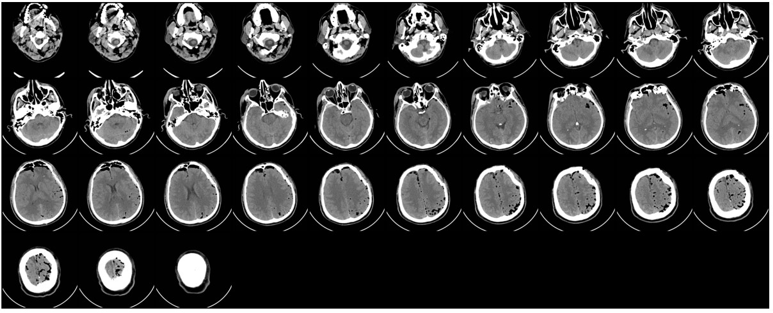
\includegraphics[width=0.8\textwidth]{assets/1}
	\caption*{}
\end{figure}

\textbf{1-сурет -- Пациенттің суреттер жиынтығы}

Деректердегі әрбір суретте "patient\_id (SLICE\_ID)" форматында бірегей
атау бар.jpg", мұнда patient\_id пациенттің идентификаторын, ал
SLICE\_ID - кесілген Нөмірді білдіреді. Бұл деректерді жүйелеуге және
оларды белгілі бір пациенттермен және уақыт нүктелерімен байланыстыруға
мүмкіндік береді.

Модельдеуді бастамас бұрын, деректерді мұқият өңдеу керек. Бұл процесс
бірнеше маңызды қадамдарды қамтиды.

Шуды жою: суреттердің сапасын жақсарту үшін шуды өңдеу жүргізілді.
Кеңейту, артефактілерді жою және бинаризация сияқты морфология әдістерін
қолдана отырып, кескіндердің тазалығына қол жеткізілді. Өлшемді өзгерту:
біркелкі болу және есептеу күрделілігін азайту үшін кескіндер біркелкі
өлшемге өзгертілді. Бұл қадам кескіндерді айналдыруды, бикубикалық
интерполяция әдісін қолдана отырып олардың өлшемдерін өзгертуді және
қайта айналдыруды қамтиды. Қалыпқа келтіру: қалыпқа келтіру пиксель
мәндерін {[}0, 1{]} аралығына келтірудің маңызды кезеңі болып табылады.
Бұл деректерді стандарттауды қамтамасыз етеді және модельдік оқытуды
жақсартады {[}13{]}.

Деректерді түзету процесінде сөздік жасалды, онда әр пациент суреттердің
дұрыс сұрыпталған тізіміне сәйкес келеді. Бұл сөздік кейінгі талдау мен
модель құрудың маңызды құралына айналды.

\begin{figure}[H]
	\centering
	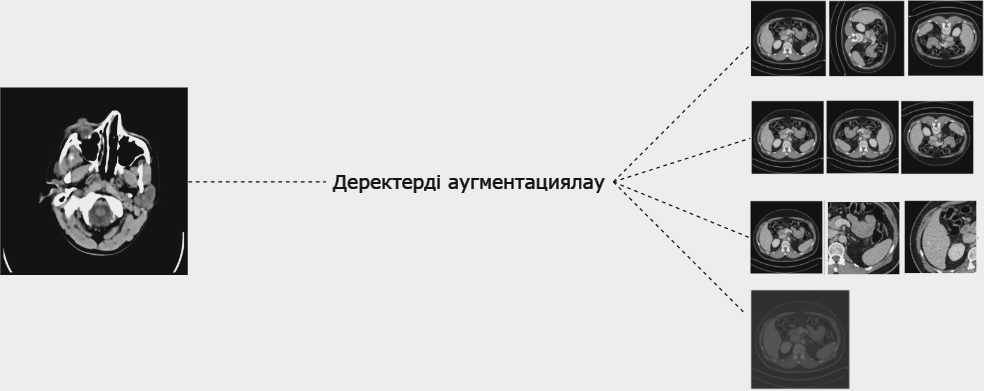
\includegraphics[width=0.8\textwidth]{assets/2}
	\caption*{}
\end{figure}

\textbf{2-сурет -- Күшейтудің қолданылуы}

Модельді оқыту үшін деректерді дайындау процесінде әдістерді қамтитын
күшейту әдісі қолданылды (2-сурет): айналу (айналу), шағылысу (флип),
ауысу (shift), масштабтау (zoom), жылжыту (shear), жарықтықты өзгерту
(brightness) және контраст (контраст). Бұл күшейту әдістері модельдің
жалпылау қабілетін жақсартуда және оның деректердің әртүрлі
вариацияларына төзімділігін арттыруда шешуші рөл атқарады {[}14{]}.

Айналу, шағылысу, жылжыту және масштабтау сияқты деректерді күшейту
әдістері оқу жинағын әртүрлі кескін вариацияларымен байытады {[}15{]},
бұл модельге әртүрлі нысан позициялары мен масштабтарында жақсырақ
үйренуге көмектеседі. Бұл модельдің нақты көріністердегі объектілерді
тану және жіктеу қабілетін жақсартуға ықпал етеді.

Сонымен қатар, жарықтық пен контрастты өзгерту әдістері әртүрлі
жарықтандырумен және контрастпен кескіндер жасауға мүмкіндік береді, бұл
сонымен қатар, модельге әртүрлі жарық жағдайларында үйренуге
көмектеседі. Бұл модельдің жарықтандырудың өзгеруіне төзімділігін
арттырады және нақты жұмыс жағдайында тұрақты нәтижелерді қамтамасыз
етеді.

Тұтастай алғанда, осы әдістерді қолдана отырып, деректерді күшейтуді
қолдану әртүрлі және репрезентативті оқыту деректер жиынтығын құруға
ықпал етеді, бұл өз кезегінде модельдің жалпылау қабілетін жақсартады
және нақты жағдайларда деректердің әртүрлі вариацияларымен жұмыс істеу
кезінде оның тиімділігін арттырады.

Ми инсультін диагностикалау саласында терең оқыту модельдерінің озық
архитектуралары кеңінен қолданылады {[}16{]}. Бұл шолуда біз негізгі
архитектураны қарастырамыз - көлемдегі медициналық кескіндерді талдауға
арналған 3D конволюциялық нейрондық желі (3D CNN). Бұл желі белгілерді
анықтауда керемет тиімділікті көрсетеді және ми инсультін дәл
диагностикалауға мүмкіндік береді.

3D CNN-медициналық суреттер сияқты үш өлшемді деректермен жұмыс істеуге
арнайы бейімделген классикалық конволюциялық нейрондық желі
архитектурасының дамуы. Ол үш өлшемді кеңістіктегі кеңістіктік және
уақыттық белгілерді бөлектеу үшін үш өлшемді конволюцияларды пайдалану
идеясына негізделген. 3D cnn негізгі ерекшеліктері:

\begin{enumerate}
\def\labelenumi{\arabic{enumi}.}
\item
  Үш өлшемді конволюциялар: 3D CNN көлемді деректерді талдау үшін үш
  өлшемді конволюцияларды пайдаланады. Бұл уақыт осі бойындағы
  кеңістіктік тәуелділіктер мен белгілердің өзгеруін ескеруге мүмкіндік
  береді.
\item
  Пулинг: конволюцияларға ұқсас, көлемді пиллинг операциялары есептеу
  көлемін азайтуға және негізгі белгілерді алуға көмектесетін
  деректердің өлшемін азайту үшін қолданылады.
\item
  Адаптивті архитектура: 3D CNN кіріс деректерінің өлшемдері мен
  пішімдерінің өзгеруіне оңай бейімделеді, бұл оны әртүрлі өлшемдегі
  медициналық кескіндерді талдаудың қуатты құралына айналдырады.
\end{enumerate}

Ми инсультін диагностикалауда қолдану:

\begin{enumerate}
\def\labelenumi{\arabic{enumi}.}
\item
  Ерекшеліктерді бөлектеу: 3D CNN медициналық суреттерде қанайналым
  жүйесіндегі ауытқулар немесе ми құрылымындағы өзгерістер сияқты
  сипаттамалық ерекшеліктерді ажырата алады.
\item
  Дені сау және зардап шеккен аймақтарды саралау: Архитектура инсультті
  диагностикалау үшін маңызды болып табылатын мидың қалыпты және зардап
  шеккен аймақтары арасында дәл ажыратуға мүмкіндік береді.
\item
  Кеңістіктік және уақыттық тәуелділіктерді есепке алу: 3D CNN
  деректердегі үш өлшемді кеңістіктік және уақыттық тәуелділіктерді
  тиімді қарастырады, бұл диагностиканың дәлдігін жақсартады және тіпті
  күрделі өзгерістерді анықтауға мүмкіндік береді {[}17{]}.
\end{enumerate}

Бұл жұмыста ми инсультін диагностикалау үшін 3D конволюциялық нейрондық
желі қолданылды. Бұл архитектура компьютерлік томография (CT) сияқты үш
өлшемді деректерді өңдеуге арналған қуатты құрал болып табылады
(3-сурет).

\begin{figure}[H]
	\centering
	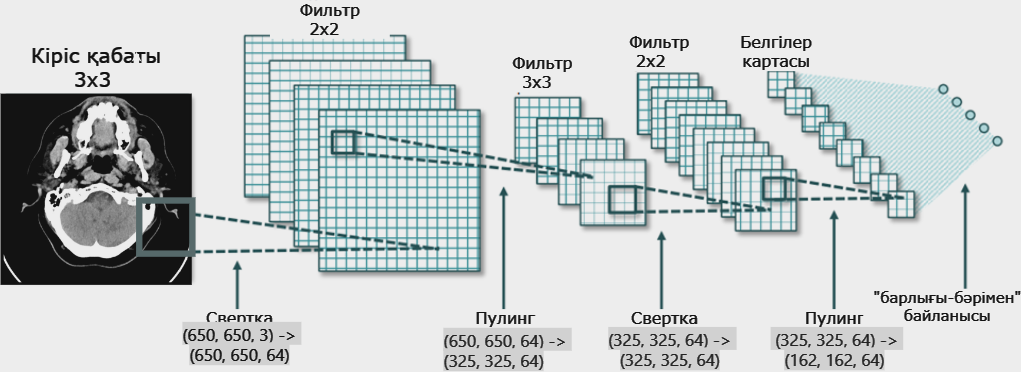
\includegraphics[width=0.8\textwidth]{assets/3}
	\caption*{}
\end{figure}

\textbf{3-сурет -- 3D CNN архитектурасы}

Бұл бөлімде ми инсультін диагностикалау үшін ұсынылған модельдің
архитектурасы қарастырылады. Негізгі құрал 3D конволюциялық нейрондық
желі болып табылады, ол үш өлшемді кірістерді тиімді өңдеуді қамтамасыз
етеді.

3D конволюциялық нейрондық желінің жұмыс принципі оның үш өлшемді
деректерді талдау қабілетінде жатыр, бұл әсіресе CT сканерлері сияқты
медициналық кескіндерді өңдеу кезінде маңызды. Бұл архитектура көлемді
деректердегі кеңістіктік ерекшеліктер мен қатынастарды алуға мүмкіндік
береді.

Модель архитектурасы бірнеше негізгі қабаттарды қамтиды, олардың
әрқайсысы деректерді өңдеу мен талдауда шешуші рөл атқарады. Кіріс
қабаты үш өлшемді CT сканерлеуді қабылдауға арналған, ал конволюция
қабаттары үш өлшемді кеңістіктен белгілерді шығарып, үш бағытта
(тереңдік, ені, биіктігі) конволюция операцияларын орындайды.

Сонымен қатар, модельге деректердің көлемін азайту және негізгі
белгілерді сақтау арқылы олардың өлшемін төмендететін Max Pooling
қабаттары сияқты кіші үлгі қабаттары кіреді. Бұл компоненттер үш өлшемді
медициналық кескіндерге негізделген тиімді оқыту мен диагностика үшін
оңтайлы архитектураны қамтамасыз етеді {[}18{]}.

Терең оқытуды қолдана отырып, ми инсультін диагностикалау жүйесін
дамытудағы маңызды қадам модельдің өнімділігін бағалау болып табылады.
Ол үшін жүйенің дәлдігін, сезімталдығын және басқа сипаттамаларын
өлшеуге мүмкіндік беретін әртүрлі көрсеткіштер мен көрсеткіштер
қолданылады. Төменде әзірленген модельдің тиімділігін бағалау үшін
қолданылатын негізгі бағалау көрсеткіштеріне шолу берілген.

Дәлдік мысалдардың жалпы санына қатысты модельдің дұрыс болжамдарының
пайызын білдіреді {[}19{]}. Бұл көрсеткіш жүйенің тиімділігінің жалпы
өлшемі болып табылады және формула бойынша есептеледі:

Дәлдік = Дұрыс болжамдардың саны/Мысалдардың жалпы саны

Шолу (немесе сезімталдық) модельдің оң жағдайларды анықтау қабілетін
өлшейді. Бұл ми инсультін диагностикалау контекстіндегі маңызды
көрсеткіш, өйткені жалған теріс нәтижелердің төмендеуі өте маңызды
{[}20{]}. Шолу формула бойынша есептеледі:

Шолу = Шынайы оң болжамдардың саны/Нақты оң жағдайлардың жалпы саны

F1-бағалау дәлдік пен шолудың орташа өлшенген мәні болып табылады. Бұл
көрсеткіш жалған оң және жалған теріс жағдайларды ескереді, бұл
теңгерімсіз деректермен жұмыс істеу кезінде оны ақпараттандырады
{[}21{]}.

\hspace{0pt} \textbf{Нәтижелер мен талқылау.} Зерттеу барысында әртүрлі
оқу параметрлерінің конфигурацияларын қолдана отырып, модель әзірленді
және оқытылды. Оқыту дәуірлерінің жалпы саны 150 болды және олардың
әрқайсысы үшін модель төрт түрлі жағдайда сыналды, соның ішінде
деректерді күшейтудің әртүрлі комбинациялары ұсынылды (1-кесте).

Күшейтудің болмауы: бұл режимде барлық күшейту қабаттары өшірілді, бұл
модельге бастапқы деректерде өзгеріссіз үйренуге мүмкіндік берді.

Негізгі күшейту: бұл режим тек жарықтық пен контрастты өзгерту
қабаттарын қамтыды. Күшейтудің бұл түрі модельге кескіндердің жарықтығы
мен контрастының өзгеруіне төзімді болуға көмектесті.

Аралық күшейту: жарықтықты, контрастты, бұрылысты, шағылысуды және орын
ауыстыруды өзгерту қабаттарын қамтыды. Ұлғайтудың бұл түрі оқу деректер
жиынтығының әртүрлілігіне ықпал етті және модельдің кірістердің әртүрлі
вариацияларына төзімділігін арттырды.

Жетілдірілген күшейту: барлық қол жетімді күшейту қабаттарын қамтыды.
Күшейтудің бұл түрі жарықтылықтың, Контрасттың, бұрылыстардың,
шағылысулардың, мещысулардың және басқа кескін түрлендірулерінің
өзгеруін қоса алғанда, оқу деректер жиынтығында максималды әртүрлілікті
қамтамасыз етті.

\textbf{1-кесте -- Күшейту түрі бойынша бағалау}

\begin{longtable}[]{@{}
  >{\raggedright\arraybackslash}p{(\columnwidth - 4\tabcolsep) * \real{0.4408}}
  >{\raggedright\arraybackslash}p{(\columnwidth - 4\tabcolsep) * \real{0.2938}}
  >{\raggedright\arraybackslash}p{(\columnwidth - 4\tabcolsep) * \real{0.2654}}@{}}
\toprule\noalign{}
\endhead
\bottomrule\noalign{}
\endlastfoot
\textbf{Күшейту түрі} & \textbf{Дәлдік} & \textbf{Шолу} \\
Күшейтудің болмауы & 0.9655 & 0.9091 \\
Негізгі күшейту & 0.9828 & 0.9545 \\
Аралық күшейту & 0.9310 & 0.8636 \\
Кеңейтілген күшейту & 0.8793 & 0.8182 \\
\end{longtable}

4-суретте модельдің 150 кезеңнен (эпохадан) өткеннен кейінгі тестілеу
нәтижесі диаграмма түрінде көрсетілген. Осыған қарай отырып, біздің
модельдің әр түрлі күшейту түріне байланысты дәлдіктің әртүрлі болатынын
көруге болады. Күшейтудің барлық түрін қолданғанда деректердің көлемі
үлкейіп, оның дәлдікке әсер еткенін көрсетеді. Күшейтуді қоспағанда
дәлдік 97\% және қосқанда 88\% көбейгенін көреміз.

\begin{figure}[H]
	\centering
	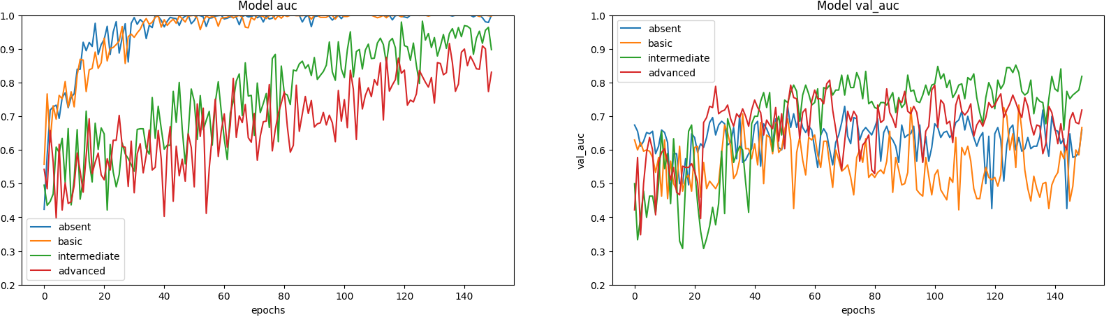
\includegraphics[width=0.8\textwidth]{assets/4}
	\caption*{}
\end{figure}

(a)

\begin{figure}[H]
	\centering
	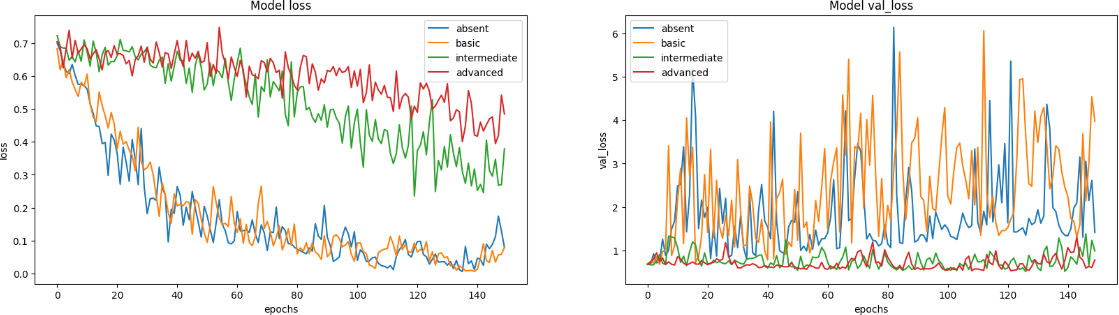
\includegraphics[width=0.8\textwidth]{assets/5}
	\caption*{}
\end{figure}

(b)

\textbf{4-сурет -- 150 эпохадағы модельді сынау (a) дәлдік (b) тестілеу
және валидация}

\textbf{кезіндегі шығын}

Оқу процесі аяқталғаннан кейін модельдің тиімділігінің ақпараттық
көрінісін жасауға болады. Валидациялық деректер жиынтығындағы
теңгерімсіздікті ескере отырып, жоғарыда айтылғандай, ROC (ROC AUC)
қисығының астындағы аймақ қолданылады. Бұл метрикалық көрсеткіш
модельдің сезімталдықты да, ерекшелікті де ескере отырып, әртүрлі
сыныптар арасындағы айырмашылықты анықтау қабілетін жан-жақты бағалауды
қамтамасыз етеді. ROC AUC модельдің кемсітушілік қабілетіне нюансты баға
береді, әсіресе сыныпты бөлуде теңгерімсіздік бар сценарийлерде құнды.

Зерттеу нәтижелері ми инсультін диагностикалау үшін әзірленген модельдің
өнімділігіне әртүрлі деректерді күшейту әдістерінің айтарлықтай әсерін
көрсетеді. Эксперименттер күшейтудің төрт түрін талдады: күшейтудің
болмауы, негізгі күшейту, аралық күшейту және кеңейтілген күшейту.

Деректерді күшейтуді қолданбай оқытылған Модель жоғары дәлдікті
(96.55\%) және шолуды (90.91\%) көрсетті. Алайда, күшейтудің әртүрлі
түрлерін қосу нәтижелердің одан әрі жақсаруына әкелді. Мысалы, негізгі
күшейтуді қолдана отырып дайындалған модель дәлдікті (98.28\%) және
шолуды (95.45\%) көрсетті. Бұл суреттердің жарықтығы мен контрастын
өзгерткен кезде модельдің деректерді дұрыс жіктеу қабілетінің
айтарлықтай жақсарғанын көрсетеді.

Айта кету керек, айналу, шағылысу және орын ауыстыру сияқты қосымша
кескін түрлендірулерін қамтитын аралық және кеңейтілген күшейтуді
қолдану модельдің өнімділігін жақсартуға әкелді. Алайда, жетілдірілген
күшейтуді қолдану кезінде басқа күшейту түрлерімен салыстырғанда
дәлдіктің (87.93\%) және шолудың (81.82\%) шамалы төмендеуі байқалды.

4-суреттегі нәтижелерді талдау 150 оқу дәуіріндегі модельдің өнімділігін
нақты салыстыруға мүмкіндік береді. Дәлдік графиктері мен жоғалту
функциялары әр түрлі күшейту әдістерін қолдану түпкілікті нәтижеге
айтарлықтай әсер ететіндігін көрсетеді. Бұл терең оқыту модельдерін
оқыту үшін деректерді күшейту стратегиясын дұрыс таңдаудың маңыздылығын
растайды.

Сонымен қатар, бұл зерттеу модельдің сезімталдық пен ерекшелікті ескере
отырып, сыныптарды ажырату қабілетін бағалау үшін ROC қисығының
астындағы аймақ метрикасын (ROC AUC) пайдаланды. Нәтижелер модельдің
жоғары кемсітушілік қабілетін көрсетеді, әсіресе сынып теңгерімсіздігі
жағдайында.

Осылайша, нәтижелер терең оқытуды пайдалана отырып, ми инсультін
диагностикалау үлгісінің өнімділігін жақсарту үшін әртүрлі деректерді
күшейту стратегияларын қолданудың тиімділігін растайды.

\textbf{Қорытынды.} Қорытындылай келе, терең оқытуды қолдана отырып, ми
инсультін диагностикалау саласындағы зерттеудің маңыздылығын атап өткен
жөн. Заманауи технологиялардың дамуы осы ауыр неврологиялық ауруды
диагностикалаудың дәлдігі мен тиімділігін жақсартатын инновациялық
тәсілдерді қолдануға мүмкіндік береді.

Әзірленген 3D конволюциялық нейрондық желі инсульт белгілерін тезірек
және дәл анықтауға ықпал ететін мидың компьютерлік томографиясын
автоматтандырылған өңдеу мен талдаудың перспективалы құралын ұсынады. Әр
түрлі модельдік архитектуралармен және оқыту әдістерімен тәжірибе жасау
оқыту мен деректерді өңдеу процесін оңтайландыруға бағытталған
тәсілдердің маңыздылығын көрсетеді.

Деректерді күшейтуді қолдану және әртүрлі қабаттарды қолдану модельдің
әртүрлі сканерлеу жағдайларына төзімділігін арттырады және оның жалпылау
қабілетін арттыруға көмектеседі. Деректерді мұқият өңдеу, соның ішінде
шуды жою, өлшемін өзгерту және қалыпқа келтіру модельді жақсартуға
айтарлықтай үлес қосты.

Өнімділік көрсеткіштерімен өлшенген валидациялық деректерден алынған
нәтижелер ми инсультін диагностикалау мәселесін шешу үшін ұсынылған
модельдің әлеуетін көрсетеді. Осы саладағы зерттеулердің одан әрі дамуы
инсультпен ауыратын науқастарды диагностикалау мен емдеуде дәрігерлерді
қолдау үшін дәлірек және сенімді құралдарды жасауға әкелуі мүмкін.

\textbf{Әдебиеттер}

1.Feigin V.L., Owolabi M.O., Abanto C., Addissie A., Adeleye A.O.,
Adilbekov Y., Topcuoglu M.A. Pragmatic Solutions to Reduce the Global
Burden of Stroke: A World Stroke Organization---Lancet Neurology
Commission.//~Lancet Neurol.~2023;10:142--149.

DOI10.1016/S1474-4422(23)00277-6.~

2.Feigin V.L., Brainin M., Norrving B., Martins S., Sacco R.L., Hacke
W., Lindsay P. World Stroke Organization (WSO): Global Stroke Fact Sheet
2022.~//Int. J. Stroke.-~2022.-Vol.17.- P.18--29.
doi:~10.1177/17474930211065917.~

3.Amiri Z, Heidari A, Navimipour NJ, Unal M, Mousavi A.~Adventures in
data analysis: a systematic review of deep learning techniques for
pattern recognition in cyber-physical-social systems.~//Multimed Tools
and Applications.- 2023.- Vol.21(23):42.DOI 10.1007/s11042-023-16382-x

4.Sudheer Kumar E, Shoba Bindu C.~Medical image analysis using deep
learning: a systematic literature review//~In book: Emerging
Technologies in Computer Engineering: Microservices in Big Data
Analytics.-2019.- P.81-97. DOI 10.1007/978-981-13-8300-7\_8

5.Ortiz G.A., Sacco R.L. National Institutes of Health Stroke Scale
(NIHSS) In: D'Agostino R.B., Sullivan L., Massaro J., editors.~Wiley
Encyclopedia of Clinical Trials.~Wiley-Interscience; Hoboken, NJ, USA:
2008. pp. 1--9.~{[}Google Scholar{]}

6.Assayony et al M. O., Mahmoud S. Recognition of Arabic handwritten
words using gabor-based bag-of-features
framework.//\emph{~}International Journal of Computing and Digital
Systemss.-\emph{~}2018.-Vol.7(1).- P.35-42. DOI 10.12785/ijcds/070104.

7.Kothari R.U., Pancioli A., Liu T., Brott T., Broderick J. Cincinnati
Prehospital Stroke Scale: Reproducibility and Validity.~//Ann.
Emerg.Med.\emph{-}1999.-Vol.33(4).- P.373-378

DOI 10.1016/S0196-0644(99)70299-4.

8.Rao C., Liu Y. Three-dimensional convolutional neural network (3D-CNN)
for heterogeneous material homogenization.// Computational Materials
Science.-2020.-Vol.184. Elsevier

https://doi.org/10.1016/J.COMMATSCI.2020.109850 109850

9.Wang J., Zhu H., Wang S.H., Zhang Y.D. A Review of Deep Learning on
Medical Image Analysis //Mob. Netw. Appl.-\emph{~}2021.-Vol.26.-
P.351-380. DOI 10.1007/s11036-020-01672-7.~

10.Barragán-Montero A, Javaid U, Valdés G, Nguyen D, Desbordes P, Macq
B, et al..~Artificial intelligence and machine learning for medical
imaging: a technology review.//~\emph{Phys Med}, 2021- Vol.~83.-
P.242--256. DOI 10.1016/j.ejmp.2021.04.016.

11.Zhang Y., Liu S., Li C., Wang J. Application of Deep Learning Method
on Ischemic Stroke Lesion Segmentation.//~J. Shanghai Jiaotong Univ.
(Sci.), ~2022.- Vol.27.- P.99--111. DOI 10.1007/s12204-021-2273-9.~

12.Wen L., Li X., Li X., Gao L. A new transfer learning based on VGG-19
network for fault diagnosis // Proceedings of the 2019 IEEE 23rd
international conference on computer supported cooperative work in
design (CSCWD). 2019. - P. 205--209.~DOI 10.1109/CSCWD.2019.8791884

13.Chen C., Yuan K., Fang Y., Bao S., Tong R.K.Y. Hierarchically Spatial
Encoding Module for Chronic Stroke Lesion Segmentation// Proceedings of
the 2021 10th International IEEE/EMBS Conference on Neural Engineering
(NER).- 2021.- P. 1000--1003. {[}Google Scholar{]}

14.Kaya A., Keceli A. S., Catal C., Yalic H. Y., Temucin H.,
Tekinerdogan B. Analysis of transfer learning for deep neural network
based plant classification models.//~Computers and Electronics in
Agriculture\emph{,~}2019. Vol.158.-P.20--29.
DOI~10.1016/j.compag.2019.01.041.~

15.Zhao W., Du S. Spectral--spatial feature extraction for hyperspectral
image classification: a dimension reduction and deep learning approach
\emph{//}IEEE Transactions on Geoscience and Remote Sensing\emph{,}
2016.- Vol.54(8).- P.4544 - 4554. DOI10.1109/tgrs.2016.2543748.~

16.Van der Velden BH, Kuijf HJ, Gilhuijs KG, Viergever MA.~Explainable
artificial intelligence (XAI) in deep learning-based medical image
analysis.//~Med Image Anal.,2022.- Vol.~79:102470. DOI
10.1016/j.media.2022.102470

17.Litjens G, Kooi T, Bejnordi BE, Setio AAA, Ciompi F, Ghafoorian M, et
al..~A survey on deep learning in medical image analysis.//~Med Image
Anal.,2017.- Vol.~42.- P.60-88.

DOI 10.1016/j.media.2017.07.005

18. Kuo C.F.J., Liao Y.S., Barman J., Liu S.C. Semi-supervised deep
learning semantic segmentation for 3D volumetric computed tomographic
scoring of chronic rhinosinusitis: Clinical correlations and comparison
with Lund-Mackay scoring.~//Tomography.-\emph{~}2022. Vol.8.-
P.718--729. DOI 10.3390/tomography8020059.~

19.De Santis D., Polidori T., Tremamunno G., Rucci C., Piccinni G.,
Zerunian M., Pugliese L., Del Gaudio A., Guido G., Barbato L., et al.
Deep learning image reconstruction algorithm: Impact on image quality in
coronary computed tomography angiography.//~La Radiol.
Medica.~-2023.-Vol.128(4).- P.434 - 444. DOI
10.1007/s11547-023-01607-8.~

20.Ding Q., Nan Y., Gao H., Ji H. Deep learning with adaptive
hyper-parameters for low-dose CT image reconstruction //~IEEE Trans.
Comput. Imaging.- \emph{~}2021.-Vol.7.-P.648 - 660.

DOI 10.1109/TCI.2021.3093003.~

21.Capps M., Mueller J.L. Reconstruction of organ boundaries with deep
learning in the D-bar method for electrical impedance tomography//~IEEE
Trans. Biomed. Eng.,\emph{~}2020.- Vol.68.-P.826--833.
10.1109/TBME.2020.3006175.~

\emph{\textbf{Авторлар туралы мәліметтер}}

Жантөре М.Қ. -- магистрант, әл-Фараби атындағы Қазақ ұлттық
университеті, Алматы, Қазақстан,

e-mail:marlenzantore@gmail.com;

Омаров Б.С.- PhD, доцент, әл-Фараби атындағы Қазақ ұлттық университеті,
Алматы, Қазақстан, e-mail:batyahan@gmail.com;

Зиятбекова Г.З.- PhD, м.а. доцент, әл-Фараби атындағы Қазақ ұлттық
университеті, Алматы, Қазақстан, Казахстан, e-mail:ziyatbekova@mail.ru;

Бидахмет Ж. -PhD, м.а. доцент, әл-Фараби атындағы Қазақ ұлттық
университеті, Алматы, Қазақстан, e-mail:bidakhmetzhanar@gmail.com

\emph{\textbf{Information about the authors}}

M.Zhantore - graduate student at Al-Farabi Kazakh National University,
Almaty, Kazakhstan,

e-mail:marlenzantore@gmail.com;

B.Omarov -PhD, Associate Professor Al-Farabi Kazakh National University,
Almaty, Kazakhstan,

e-mail:batyahan@gmail.com;

G. Ziyatbekova - PhD, Acting Associate Professor Al-Farabi Kazakh
National University, Almaty, Kazakhstan,

e-mail:ziyatbekova@mail.ru;

Zh. Bidakhmet - PhD, аcting Associate professor Al-Farabi Kazakh
National University, Almaty, Kazakhstan,

e-mail:bidakhmetzhanar@gmail.com

IRSTI 50.47.29

\textbf{DEVELOPMENT OF AN ALGORITHM FOR ADAPTING A MATHEMATICAL MODEL OF
THE PROCESS OF MIXING AND MELTING COPPER CONCENTRATES}

\textbf{U. Imanbekova\textsuperscript{1}, A.
Kalizhanova\textsuperscript{2,1}, A.Kozbakova\textsuperscript{2,3}, A.
Imanbekova\textsuperscript{4}, A.Utegenova\textsuperscript{1,2}}

\textsuperscript{1}Almaty University of Power Engineering and
Telecommunications named after G.Daukeyev, Almaty, Kazakhstan,

\textsuperscript{2}Institute of Information and Computational
Technologies CS MSHE RK, Almaty, Kazakhstan,

\textsuperscript{3}Almaty Technological University, Almaty, Kazakhstan,

\textsuperscript{4}Taraz Regional University named after M.Kh. Dulaty,
Taraz, Kazakhstan,

е-mail: uli.08@mail.ru

The paper describes the information base of the system, which is formed
by algorithms of centralized control, automated analytical control
system and control data of material flows. The data processing algorithm
according to a special program generates additional information
necessary to solve the control tasks of the system and includes
algorithms for processing analytical data information, as well as data
for monitoring material flows, calculations of additional electric
furnace variables, loading of charge into furnace bunkers and
technological variables by department. The simulation model of the
functioning of the complex "technological process -- control system" is
implemented in the form of a package of interconnected software modules.
The package implementing the simulation model is divided into three
complexes: a set of programs for "Data collection and processing"; a
complex for "Optimal process control"; a set of programs for "optimal
energy regime management".

\textbf{Keywords.} Copper raw materials, blending, smelting,
mathematical model, mixing and melting.

\begin{quote}
\textbf{МЫС КОНЦЕНТРАТТАРЫН АРАЛАСТЫРУ ЖӘНЕ БАЛҚЫТУ ПРОЦЕСІ ҮШІН
МАТЕМАТИКАЛЫҚ МОДЕЛЬДІ БЕЙІМДЕУ АЛГОРИТМІН ӘЗІРЛЕУ}

\textbf{У.Иманбекова\textsuperscript{1},А.Калижанова\textsuperscript{2,1},
А.Козбакова\textsuperscript{2,3}, А.Иманбекова\textsuperscript{4},
А.Утегенова\textsuperscript{1,2}}
\end{quote}

\textsuperscript{1}Ғ.Дәукеев атындағы Алматы энергетика және байланыс
университеті, Алматы, Қазақстан,

\textsuperscript{2}Ақпараттық және есептеуіш технологиялар институты ҚР
ҒЖБМ ҒК, Алматы, Қазақстан,

\textsuperscript{3}Алматы технологиялық университеті, Алматы, Қазақстан,

\textsuperscript{4}М.Х. Дулати атындағы Тараз өңірлік университеті,
Тараз, Қазақстан,

е-mail: uli.08@mail.ru

Мақалада орталықтандырылған басқару алгоритмдерімен, аналитикалық
бақылаудың автоматтандырылған жүйесімен және материалдық Ағындарды
бақылау деректерімен қалыптасатын жүйенің ақпараттық базасы сипатталған.
Арнайы бағдарлама бойынша деректерді өңдеу алгоритмі жүйені басқару
мәселелерін шешу үшін қажетті қосымша ақпаратты жасайды және
аналитикалық ақпаратты өңдеу алгоритмдерін, сондай-ақ материалдық
Ағындарды бақылау, электр пешінің қосымша параметрлерін есептеу, пештің
бункерлеріне шихтаны жүктеу және цехтар бойынша технологиялық
параметрлерді қамтиды. «Технологиялық процесс -- басқару жүйесі»
кешенінің жұмыс істеуінің имитациялық моделі өзара байланысты
бағдарламалық модульдер пакеті түрінде іске асырылды. Модельдеу моделін
жүзеге асыратын Пакет үш кешенге бөлінеді: «деректерді жинауға және
өңдеуге» арналған бағдарламалар жиынтығы; «технологиялық процесті
оңтайлы басқаруға» арналған кешен; «оңтайлы энергетикалық режимді
басқаруға» арналған бағдарламалар жиынтығы.

\textbf{Түйін сөздер:} мыс шикізаты, араластыру, балқыту, математикалық
модель, араластыру және балқыту.

\begin{quote}
\textbf{РАЗРАБОТКА АЛГОРИТМА АДАПТАЦИИ МАТЕМАТИЧЕСКОЙ МОДЕЛИ ДЛЯ
ПРОЦЕССА СМЕШИВАНИЯ И ПЛАВЛЕНИЯ МЕДНЫХ КОНЦЕНТРАТОВ}

\textbf{У.Иманбекова\textsuperscript{1},А.Калижанова\textsuperscript{2,1},
А.Козбакова\textsuperscript{2,3}, А.Иманбекова\textsuperscript{4},
А.Утегенова\textsuperscript{1,2}}

\textsuperscript{1}Алматинский университет энергетики и связи им. Г.
Даукеева, Алматы, Казахстан.

\textsuperscript{2}Институт информационных и вычислительных технологий
КН МНВО РК, Алматы, Казахстан,

\textsuperscript{3}Алматинский технологический университет, Алматы,
Казахстан,

\textsuperscript{4}Таразский региональный университет им.М. Х. Дулати,
Тараз, Казахстан,
\end{quote}

е-mail: uli.08@mail.ru

В статье описана информационная база системы, которая формируется
алгоритмами централизованного управления, автоматизированной системой
аналитического контроля и данными контроля материальных потоков.
Алгоритм обработки данных по специальной программе генерирует
дополнительную информацию, необходимую для решения задач управления
системой, и включает в себя алгоритмы обработки аналитической
информации, а также данные для мониторинга материальных потоков,
расчетов дополнительных параметров электропечи, загрузки шихты в бункеры
печи и технологических параметров по цехам. Имитационная модель
функционирования комплекса "технологический процесс -- система
управления" реализована в виде пакета взаимосвязанных программных
модулей. Пакет, реализующий имитационную модель, разделен на три
комплекса: набор программ для "Сбора и обработки данных"; комплекс для
"Оптимального управления технологическим процессом"; набор программ для
"управления оптимальным энергетическим режимом".

\textbf{Ключевые слова.} Медное сырье, смешивание, плавка,
математическая модель, смешивание и плавка.

\textbf{Introduction.} To predict process variables using an adaptive
mathematical model, constant updated samples containing a certain number
of observations of the process must be stored in the PC memory {[}1{]}.
When the operator enters the code of a certain equation of the model,
the corresponding values of the model parameters, object variables and
algorithm constants are received at the algorithm input, the adjusted
model parameters and the predicted value of the object variable are
printed {[}2{]}.

The analytical information processing algorithm generates information
about the chemical compositions of material flows necessary for solving
functional control tasks using information arrays generated by an
automated analytical control system based on \emph{X-ray} spectral
equipment {[}3{]}. The data is sent to the computer of the automated
control system of the metallurgical workshop via interprocessor
communication channels as they are formed. The data on the chemical
composition of the melting products relate to the moments of discharge
of these products, which are random in nature {[}4{]}. The output
information of the algorithm is preprocessed information about the
chemical composition of material flows {[}5{]}.

Based on the data of the daily work schedule of the electric furnace
department, which determines the number of processed granules,
revolutions, limestone, liquid converter slag, a given electrical power,
taking into account the current chemical composition of the loaded
materials, a table of initial data was filled in, which were transmitted
via communication channels to the information and computing center
{[}6{]}. The obtained data of the optimal technological regime were
printed out and transmitted to the shift foreman in the form of a task
for implementation during the process {[}7{]}.

\textbf{Materials and methods.} During the tests, the following values
characterizing the electric melting process were recorded in the
observation log: date and shift number, set and actual, number of loaded
materials (by type), power consumption, electric power of the furnace,
current and voltage at the electrodes, the amount of matte produced, the
amount of fused slag; the results of chemical analyses of the loaded
materials and the products received; the surname of the replacement
master; the time of solving the problem on the PC {[}8{]}.

The tests were carried out in two stages: at the first, data was
collected during the usual (existing) control of the electric welding
process, at the second -- during the implementation of the process
according to the optimal control algorithm {[}9{]}.

The choice of a working algorithm for adapting a mathematical model that
best satisfies the condition of accuracy of approximation by the model
of the output variables of an object over a time interval of length is
reduced to determining the type of operators
\(\psi\{.\},\left\{ . \right\}\) of the sequence type
\(\gamma\lbrack k\rbrack\), the value of constants \(\eta\), and the
minimum sample length {[}10{]}.

We present a working algorithm for adapting the mathematical model of
electric melting.

The adaptation algorithm calculates the current values of the parameters
of the mathematical model based on the initial data:

a) the current values of the output and input variables of the adapting
equation (model).

b) the values of the parameters obtained at the previous step of the
algorithm;

c) values of constants;

d) the calculated value of the output variable obtained at the previous
step of the algorithm.

The output information of the algorithm is the adjusted values of the
equation parameters to the following Equation 1.

\begin{quote}
\(\xi = \delta_{0} + \sum_{i = 1}^{m}\delta_{i}\psi_{i}\) (1)
\end{quote}

Minimizing the square of the mismatch between the actual (measured at
the nth instant of time) value of the output variable to its calculated
value to the following Equation 2.

\(\Delta\xi = (\xi\lbrack n\rbrack - \delta_{0} - \sum_{i = 1}^{m}{\delta_{i}\psi_{i}}\lbrack n\rbrack)^{2}\)
(2)

Where \(\xi\lbrack n\rbrack\) is the output variable of the model, Here:

\(\psi_{i}\lbrack n\rbrack,(i = \overline{1,m})\) - input variables of
the model,

n=1,2,... - discrete time,

\(\delta_{0},\delta_{i}(i = \overline{1,m})\) - equation parameters.

Calculation formulas to the following Equations 3-10:

\begin{quote}
\(\langle\frac{\delta_{o}\lbrack k\rbrack = \delta_{o}\lbrack k - 1\rbrack + t\lbrack k\rbrack\gamma_{o}\lbrack k\rbrack\Delta\varepsilon\lbrack n,k - 1\rbrack}{\delta_{i}\lbrack k\rbrack = \delta_{i}\lbrack k - 1\rbrack + t\lbrack k\rbrack\gamma_{i}\lbrack k\rbrack\Delta\varepsilon\lbrack n,k - 1\rbrack\psi_{i}\lbrack n\rbrack}\)\begin{figure}[H]
	\centering
	
\includegraphics[width=0.8\textwidth]{assets/6}
	\caption*{}
\end{figure}
(3)
\end{quote}

\(\delta_{i}\lbrack k\rbrack = \delta_{i}\lbrack k - 1\rbrack(i = 0,1,...),\)
(4)

\(\Delta\varepsilon\lbrack n,k\rbrack = \overline{\varepsilon}\lbrack n\rbrack - \breve{\varepsilon}\lbrack n,k\rbrack\)
(5)

\(\breve{\varepsilon}\lbrack n,k\rbrack = \delta_{0}\lbrack k\rbrack + \sum_{i = 1}^{m}{\delta_{i}\lbrack k\overline{\rbrack\psi}\lbrack n\rbrack}\)
(6)

\(\overline{\varepsilon}\lbrack n\rbrack = \overline{\varepsilon}\lbrack n - 1\rbrack + \frac{1}{T_{\varepsilon}}(\varepsilon\lbrack n\rbrack - \overline{\varepsilon}\lbrack n - 1\rbrack\),
\((i = \overline{1,m)}\) (7)

\(\overline{\varepsilon}\lbrack n\rbrack = \overline{\varepsilon}\lbrack n - 1\rbrack + \frac{1}{T_{\varepsilon}}(\varepsilon\lbrack n\rbrack - \overline{\varepsilon}\lbrack n - 1\rbrack)\)
(8)

\(t\lbrack k\rbrack = 1 + r/\Delta\varepsilon\lbrack n - 1,k - 1\rbrack + \Delta\varepsilon\lbrack n - 2,k - 2\rbrack\)
(9)

\(\gamma_{i}\lbrack k\rbrack = \left( \begin{aligned}
 & \overline{\gamma_{i}} = const\ if\ \eta\lbrack\gamma\rbrack = 1 \\
 & \frac{\gamma_{i}\lbrack 0\rbrack}{S\lbrack n\rbrack},if\eta\lbrack х\gamma\rbrack = 0
\end{aligned} \right.\ \) (10)

Where:

\(S\lbrack n\rbrack\) - the number of steps of the algorithm after the
next violation of the condition
\(\left. \ \Delta\varepsilon\lbrack n,k\rbrack \right| \leq \Delta\).

\(\overline{\psi}\lbrack n\rbrack,\overline{\varepsilon}\lbrack n\rbrack\)
- variables formed by sliding averaging over intervals, respectively
\(T_{i}\)и \(T_{\varepsilon}\);

\(\delta_{i}\lbrack k\rbrack,(i = \overline{0,m})\) - equation
parameters corresponding to the kth step (iteration) of the algorithm;

\(\overset{̑}{\varepsilon}\lbrack n.k\rbrack\) - calculated values of the
output variable corresponding to time n, obtained using the parameters
\(\delta_{i}\lbrack k\rbrack\);

\(\gamma_{i}\lbrack k\rbrack,(i = \overline{0,m})\) - The iteration step
is positive numbers that determine the amount of parameter correction at
the kth step of the algorithm;

\(t\lbrack k\rbrack\) - accelerating multiplier;

\(\eta\lbrack\gamma\rbrack\) - a constant that defines the type of
sequence \(\gamma_{i}\lbrack k\rbrack(k = 1,2,...)\);

\(\Delta > 0\) - the threshold value of the misalignment of the value
\(\varepsilon\lbrack n\rbrack и\widetilde{\varepsilon}\lbrack n,k\rbrack\).

\textbf{Results and discussion.} The flowchart of the algorithm is
described in this way:

Block 1 performs the sequential formation of arrays necessary for
calculation from the total array of data.

Block 2 checks the completeness of information generation.

Block 3 checks the receipt of new analytical information.

The block diagram of the algorithm for processing analytical information
in Figure 1.

\begin{figure}[H]
	\centering
	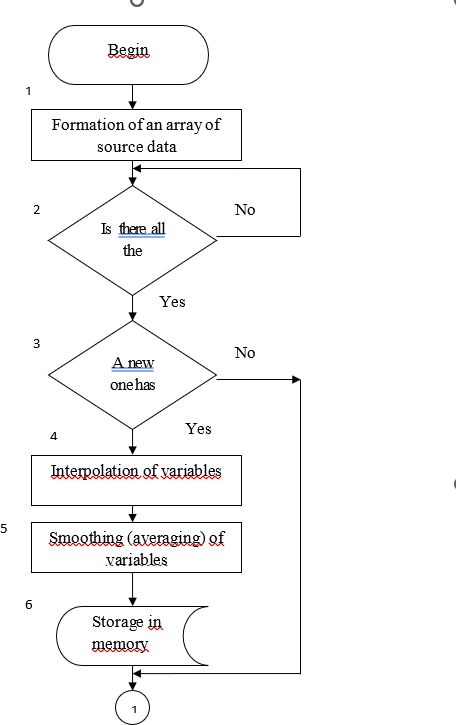
\includegraphics[width=0.8\textwidth]{assets/7}
	\caption*{}
\end{figure}

\textbf{Figure 1 - The block diagram of the algorithm for processing
analytical information}

Block 4 calculates the interpolated value of the content of the i-th
component of the j-th material of the k-th furnace to the following
Equation 11:

\begin{quote}
\(Χ_{ijk}\lbrack n\rbrack = Χ_{ijk_{}}\lbrack\mu\rbrack - \frac{\left( Χ_{ijk}\lbrack\mu\rbrack - Χ_{ijk}\lbrack\mu\rbrack \right)\left( n - \tau_{\mu} \right)}{\tau_{\mu + 1} - \tau_{\mu}}\)
(11)
\end{quote}

Where: \(X_{ijk}\lbrack\mu\rbrack\) - the content of the i-th component
in the j-th material for the k-th selection furnace;

\(\tau_{\mu},\tau_{\mu + 1}\)- accordingly, the time of the
\begin{figure}[H]
	\centering
	
\includegraphics[width=0.8\textwidth]{assets/8}
	\caption*{}
\end{figure} and
\begin{figure}[H]
	\centering
	
\includegraphics[width=0.8\textwidth]{assets/8}
	\caption*{}
\end{figure}+1 sampling of the analyzed material

\emph{n} - discrete time, the hour for which the content of the
\emph{i-th} component in the \emph{j-th} material is determined.

Block 5 performs preliminary processing of the received information --
smoothing to the following Equation 12:

\begin{quote}
\(\overline{C}\lbrack n\rbrack = \overline{C}\lbrack n - 1\rbrack + \frac{1}{T}\left( C\lbrack n\rbrack - C\lbrack n - 1\rbrack \right)\)
(12)
\end{quote}

where \(\overline{C}\lbrack n\rbrack\) - the smoothed value of the
variable at the \emph{n-th} instant of time;

\(C\lbrack n\rbrack\) - the current value of the variable at the
\emph{n-th} moment in time;

\(T\) - the smoothing interval (averaging).

Block 6 stores a sequence of values of analytical variables to the
following Equation 13:

\begin{quote}
\(C\lbrack n - 1\rbrack,\) \emph{i = 0,1,2,\ldots,N} (13)
\end{quote}

where \emph{N} is the memory depth. The average values of variables are
stored per hour, from the beginning of the shift, per shift, from the
beginning of the day, per day for each furnace.

The block diagrams of these algorithms are shown in Figure 2.

\begin{figure}[H]
	\centering
	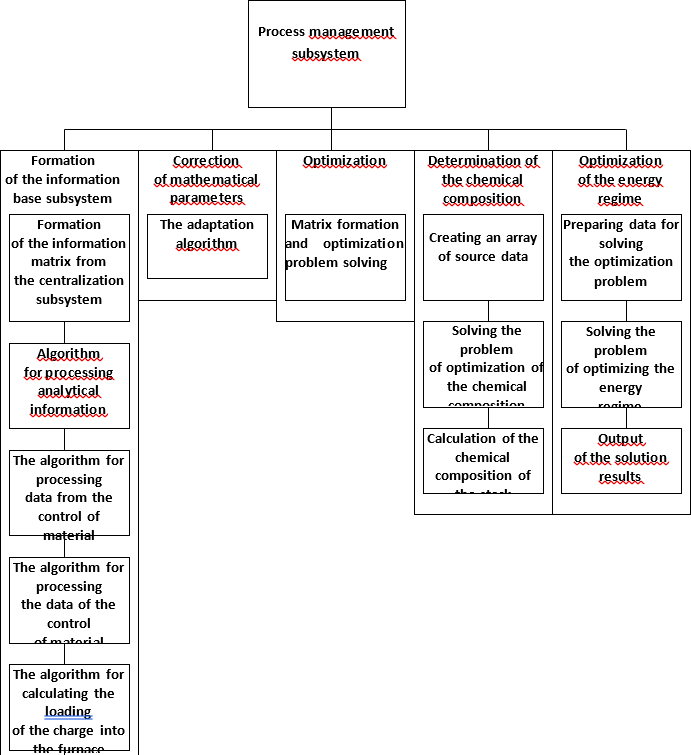
\includegraphics[width=0.8\textwidth]{assets/9}
	\caption*{}
\end{figure}

\textbf{Figure 2 - The block diagrams of these algorithms}

Block 1. Enters the values of these variables
\(X_{ij},\ Y_{ij},\ a_{ij}\) into the machine.

Block 2. Checking the values of variables for validity.

Block 3. Checking for data sufficiency, in case of insufficiency, the
display unit 4 is triggered.

Block 5. The average values of the variables are found.

Block 6. The solution of equations is performed with the previous values
of the coefficients, the calculated \(\overline{y}\ \lbrack n\rbrack\)
data are compared with the experimental
\(\overline{y}\ \lbrack n,K\rbrack\).
\(\mathrm{\Delta}y\lbrack n,K\rbrack = \overline{y}\ \lbrack n\rbrack - \overline{y}\ \lbrack n,K\rbrack\)
is calculated.

Block 7. The comparison block. If the condition
\textbar∆y{[}n,K{]}\textbar≥∆ is fulfilled, block 8 is executed, which,
using block 9, leads to an adaptation, as a result of which new
coefficient values are obtained.

Block 10. Calculation of the optimal composition of the charge. At the
same time, we use the "Optimization" subroutine of block 11.

The algorithm for adapting the mathematical model of the process of
mixing and melting copper concentrates is given below to the following
Equations 14-25:

\begin{quote}
\(f_{FeS}^{III} = \alpha_{FeS}^{II - III}G_{FeS}^{II} - K_{C}G_{FeS} - K_{mech}G_{FeS}^{III} - \alpha_{FeS}^{III - IV}\frac{\vartheta_{K}}{H_{sl}} = 0\)
(14)
\end{quote}

\(f_{Cu_{2}S}^{II} = \alpha_{Cu_{2}s}^{II - III}G_{Cu_{2}S}^{II} - K_{C}G_{Cu_{2}S} - G_{Cu_{2}S}G_{FeO} - K_{mech}G_{Cu_{2}S}^{III} - \alpha_{Cu_{2}S}^{III - IV}G_{Cu_{2}s}^{III}\frac{\vartheta_{K}}{H_{sl}} = 0\)
(15)

\begin{quote}
\(f_{CaO}^{III} = \alpha_{CaO}^{II - III}G_{CaO} + \gamma_{CaO}^{K}G^{K} - \gamma_{CaO}G_{sl}^{m} = 0\)
(16)

\(f_{SO_{2}}^{III} = \alpha_{SiO_{2}}^{II - III}G_{SiO_{2}}^{II} + \gamma_{SiO_{2}}^{K}G^{K} - \gamma_{SiO_{2}}G_{sl}^{m} = 0\)
(17)

\(f_{Cao}^{II} = \alpha_{FeO}^{II - III}G_{FeO}^{II} + \gamma_{FeO}^{K}G^{K} - \gamma_{FeO}G_{sl}^{m} = 0\)
(18)

\(G_{sl}^{II} = \beta_{1}G_{Cu_{2}S}^{III} + \beta_{2}G_{Cu_{2}O}^{III} + \beta_{3}G_{cp}^{III}\)
(19)

\(С_{sl}^{II} = \gamma_{n}G_{Cu}^{III}\) (20)

\(F_{sl}^{II} = \rho_{sl}^{R} + k_{1}G_{SiO_{2}} + k_{2}G_{CaO} + k_{3}G_{FeO} + k_{4}t_{sl}\)
(21)
\end{quote}

\(f_{sl}^{II} = K_{э}\rho_{sl}^{R}I^{2} + G_{sl}^{K}С_{sl}^{к}t_{sl}^{K} - \alpha(t_{sl} - t_{m})ц_{0}С_{sl}F_{m} - \alpha(t_{sl} - t_{st})F_{st} - G_{sl}^{m}С_{sl}t_{sl} - \sum_{е}^{}\alpha_{е}^{III - IV}G_{e}C_{e}t_{sl}\frac{\vartheta_{к}}{Н_{sl}} = 0\)
(22)

\begin{quote}
\(f_{Cu_{2}S}^{III} = \frac{\alpha_{Cu_{2}S}^{III - IV}G_{Cu_{2}S}^{III}}{H_{sl}}\vartheta_{k - \beta_{Cu_{2}S}G_{st}^{m}} = 0\)
(23)

\(f_{FeS}^{II} = \frac{\alpha_{Cu_{2}S}^{III - IV}G_{Cu_{2}S}^{III}}{H_{sl}}\vartheta_{К} - \beta_{FeS}G_{st}^{вm} = 0\)
(24)
\end{quote}

\(f_{Fe}^{II} = (\sum_{l}^{}{\gamma_{l}G_{st}C_{е}})t_{sl} + \alpha(t_{sl} - t_{st})F_{st} - \lambda(\frac{t_{st} - t_{sl}}{\delta})h_{st}S_{n} - \frac{\lambda'}{\delta}(t_{st} - t_{n})F_{n} = 0\)
(25)

The block diagram of the algorithm for optimal control of the energy
regime can be described as follows:

Blocks 1-6 . Collects, processes and generates mass data.

Blocks 7-20. The equations of the mathematical model of the electric
melting process are being implemented. The input of the blocks receives
information about the input parameters
\(\overline{G},\ \overline{H},\ \overline{U},\ \overline{H}\ Q_{c},\ G_{5_{p}}\)

Block 7. The equations of the material balance of the process are
implemented.

Block 8. The equations of the thermal process are calculated.

Block 9. Dependence of the resistivity of the charge and slag on the
input parameters determined on the basis of a study of factory slags.

Block 10. The equation of the dependence of the height of the slag bath
on the input parameters.

Block 11. Expression of the dependence of the slope depth on the input
parameters.

Blocks 12-16. The resistances of the equivalent electrical circuit of
the furnace are calculated as a function of the geometric parameters of
the specific resistances of the slag and charge and the phase voltage.

Block 17. The dependence of the phase power on the resistance of the
equivalent circuit and the phase voltage is realized.

Block 18. The dependence of the amount of matte on the input parameters
is determined.

Block 19. The dependences of the copper content in the dump slag on the
phase voltage and the electrode depth are realized.

Block 20. The specific consumption of electricity is determined,

Block 21. The adequacy of the mathematical model to the object is
checked. In case of inadequacy, he refers to the adaptation unit.

Block 22. The parameters of the mathematical model are adjusted
according to the well-known adaptation algorithm

Block 23. The optimal values of control actions are determined based on
the solution of the optimization problem.

Block 24. The optimization problem is solved using the Rosenbrock
method.

Block 25. The furnace operation is checked for accidents. In case of
failure to fulfill one of the conditions, a voltage reduction task is
issued.

Block 26. The actual voltage value is compared with the optimal one. In
the case of \(U_{real}\ \) going beyond the area \(|U -\)
\(U_{opt}|\varepsilon q\), a task is given to switch voltage stages in
one direction or the other.

Block 27. The actual conductivity is compared with the optimal one. In
case of going beyond the area
\(|q_{i} - q_{i\ opt}|\varepsilon q\)\emph{,} a task is given to bypass
the electrode in one direction or the other.

Block 28. The condition \(I \leq\) \(I_{con}\) is checked in the case of
a voltage increase task. If the condition is met, the voltage can be
increased.

Block 29. The position of the electrode holder is checked. If the
electrode holder is in the lowest position, a task is given to increase
the voltage. If not, the control is carried out by increasing the depth
of the electrode.

Block 30. It is checked whether the electrode holder is in the uppermost
position. If not, the electrode rises if a voltage reduction task is
issued.

Blocks 31-32. The magnitude of the control action (the number of voltage
stages) is determined and information is provided on which voltage stage
should be operated.

Blocks 33 - 34. An algorithm for direct control of electrode deepening
is implemented.

The results of processing the data obtained during the two stages of the
tests are summarized in a table. The tests showed: the adequacy of
mathematical models of the process of electric melting of copper
concentrates and control tasks for a real object; the effectiveness of
the developed algorithms and programs for solving problems of optimal
calculation of the stack composition, distribution of material flows and
energy management

The used energy mode of electric melting for copper sulfide concentrates
made it possible to reduce the copper content in dump slags by 0.18\%
(absolute) and reduce copper losses with slags by 5\% (relative),
increase the copper content in matte by 0.97\% while reducing
electricity consumption by 1.8\%.

\textbf{Conclusion.} Industrial tests and implementation of the electric
melting process control system were carried out in the electric furnace
department, pilot tests of the algorithm for controlling the process of
electric melting of copper concentrates in industrial conditions were
carried out.

The tests were carried out in order to: clarify the coefficients of the
mathematical model; verify the adequacy of the mathematical model of
control tasks; adjust algorithms and programs in industrial conditions;
verify the effectiveness of the developed algorithms and programs. The
tests were carried out in accordance with the program and methodology.

The results of theoretical and experimental studies on the control
system for the process of electric melting of copper sulfide
concentrates are the basis for the design solutions of the Institute of
Information and Computational Technologies CS MSHE RK.

\emph{\textbf{Financing.} Research were carried out within the framework
of the Grant Financing Project No. AP19679153 ``Research and development
of method and technologies for creating composite structures with
built-in photonic sensors PSBC (Photonic Smart Bragg Composites)''
Institute of Information and Computational Technologies of the Science
Committee of the Ministry of Science and Higher Education of the
Republic of Kazakhstan.}

\textbf{References}

1.Istadi I., Bindar Y. Improved cooler design of~electric~arc furnace
refractory in mining industry using thermal analysis modeling and
simulation.//Applied Thermal Engineering.- 2014.- Vol.73, Iss.1.-
P.1129-1140. https://doi.org/10.1016/j.applthermaleng.2014.08.070

2.Imanbekova U., Hotra O., Koshimbayev S., Optimal control of copper
concentrate blending and melting based on intelligent systems.// Journal
Przegląd Elektrotechniczny.2016.-Vol.8.- P.125-128.
doi:10.15199/48.2016.08.34

3.Malfliet A., Lotfian S., Scheunis L., Petkov V., Pandelaers L., Jones
P.T., Blanpain B. Degradation mechanisms and use of refractory linings
in copper production processes // Journal of the European Ceramic
Society. A critical review.- 2014.- Vol.34, Iss.3. - P. 849-876.
https://doi.org/10.1016/j.jeurceramsoc.2013.10.005

4.Cheng P., Herreros P., Lalpuria M., Grossmann I. Optimal scheduling of
copper concentrate operations under uncertainty.//Computers \& Chemical
Engineering.-2020.- Vol.140, 106919.
doi.org/10.1016/j.compchemeng.2020.106919

5.Guimarães F.Y., Santos I.D., Dutra J.B. Direct recovery of~copper~from
printed circuit boards (PCBs) powder~concentrate~by a simultaneous
electroleaching--electrodeposition~process.//
Hydrometallurgy.-2014.-Vol. 149.- P. 63-70.
https://doi.org/10.1016/j.hydromet.2014.06.005

6.Zhai Q.,Runqing Lui. Simultaneous recovery of arsenic and copper from
copper smelting slag by flotation: Redistribution behavior and toxicity
investigation. Journal of Cleaner Production. -2023.-Vol. 425, 138811
https://doi.org/10.1016/j.jclepro.2023.138811

7.Imanbekova U., Hotra O., Koshimbayev S. K., Popiel P., Tanas J.
Optimal control of blending and melting of copper concentrates.//
Proceedings of SPIE-The International Society for Optical Engineering
.-2015, 966246. DOI:10.1117/12.2205446

8.Rubanenko O. O., Komar V. O., Petrushenko O. Y., Smolarz A., Smailova
S., Imanbekova U., Determinition of similatiry criteria in optimization
tasks by means of neuro-fuzzy modelling. //Journal Przegląd
Elektrotechniczny.-2017.-Vol. 1(3).- P.95-98. DOI:10.15199/48.2017.03.22

9.Hotra O.Z., Koshimbayev S.K., Imanbekova U.N. Modelling in Matlab
using fuzzy logic for improving the economic factors of melting of
copper concentrate charge.// Actual problems of
economics.-2014.-Vol.11.-P. 380-387.

10.Da-wei~Wang,~Yan-jie~Liang. Comprehensive recovery of zinc, iron and
copper from copper slag by co-roasting with SO2--O2./ Journal of
Materials Research and Technology.-2022.- Vol.19.-P.2546-2555.
https://doi.org/10.1016/j.jmrt.2022.05.177

\emph{\textbf{Information about authors}}

U. Imanbekova -PhD, Associate Professor, Almaty University of Power
Engineering and Telecommunications named after G.Daukeyev, Almaty,
Kazakhstan, e-mail: uli.08@mail.ru;

A.Kalizhanova- Professor, Institute of Information and Computational
Technologies CS MSHE RK, Almaty, Kazakhstan, Almaty University of Power
Engineering and Telecommunications named after G.Daukeyev, Almaty,
Kazakhstan, e-mail: kalizhanova.aliya@gmail.com;

A.Kozbakova - PhD, Institute of Information and Computational
Technologies CS MSHE RK, Almaty,Kazakhstan, Almaty Technological
University, Almaty, Kazakhstan, e-mail: ainur79@mail.ru;

A.Imanbekova- Senior Lecturer, M. H. Dulati Taraz Regional University,
Taraz, Kazakhstan, e-mail: aleka.12@mail.ru;

A.Utegenova -PhD, Institute of Information and Computational
Technologies CS MSHE RK, Almaty, Kazakhstan, Almaty University of Power
Engineering and Telecommunications named after G.Daukeyev, Almaty,
Kazakhstan, e-mail: an.utegenova@aues.kz

\emph{\textbf{Сведения об авторах}}

Иманбекова У. -PhD., ассоциированный профессор, Алматинский университет
энергетики и связи им. Г. Даукеева, Алматы, Казахстан, e-mail:
uli.08@mail.ru;

Калижанова А. - к.ф.-м.н., профессор, Институт информационных и
вычислительных технологий КН МНВО РК. Алматинский университет энергетики
и связи им. Г. Даукеева, Алматы, Казахстан, e-mail:
kalizhanova.aliya@gmail.com;

Козбакова А.- PhD, Институт информационных и вычислительных технологий
КН МНВО РК, Алматинский технологический университет, Алматы, Казахстан,
e-mail: ainur79@mail.ru;

Иманбекова А.- старший преподаватель, Таразский региональный университет
им.М. Х. Дулати, Тараз, Казахстан, e-mail: aleka.12@mail.ru;

Утегенова А.-PhD Институт информационных и вычислительных технологий КН
МНВО РК, Алматинский университет энергетики и связи им. Г. Даукеева,
Алматы, Казахстан, e-mail: an.utegenova@aues.kz

\textbf{IRSTI 28.23.15}

\textbf{TARGET IDENTIFICATION AND TRACKING IN COMPLEX ENVIRONMENT}

\textbf{A.Karim, I.Muhammad}

Kazakh-British Technical University, Almaty, Kazakhstan,

e-mail: ad\_karim@kbtu.kz

This study focuses on developing advanced methods for the identification
and classification of objects in complex environments. Over the past two
years, there has been an increase in the use of advanced technologies in
various challenging scenarios. This research is centered on accurately
identifying targets and tracking them. The study addresses challenges
related to object detection in multi-dimensional and intricate settings,
taking into account natural conditions like rain and fog, as well as
technical limitations such as camera capabilities. Special emphasis is
placed on data collection for training the identification model,
followed by extensive data preprocessing, including cleaning, labeling,
and augmentation. The research employs YOLO and Deep Sort machine
learning algorithms, focusing on improving the accuracy and reliability
of target recognition and increasing data processing speed to minimize
misidentification risks. The integration of YOLO, known for its quick
real-time object detection, with Deep Sort, which excels in detailed
feature extraction and classification, forms the basis of our
methodology. This fusion is a complex combination of both
models\textquotesingle{} strengths, with YOLO quickly identifying
relevant objects and Deep Sort performing an in-depth analysis. The
experimental phase involves extensive testing of the models in varied
weather conditions and settings to evaluate performance under
challenging circumstances. This work aims to enhance object
identification techniques in complex environments, a critical aspect for
the effectiveness of various advanced operations. The findings are
expected to significantly contribute to the field by enabling quicker
and more accurate target identification.

\textbf{Keywords:} target identification, tracking, object detection,
drone reconnaissance.

\textbf{КҮРДЕЛІ ОРТАДА НЫСАНАНЫ АНЫҚТАУ ЖӘНЕ БАҚЫЛАУ}

\textbf{Ә. Кәрім, І.Мұхаммед}

Қазақ-Британ Техникалық университеті, Алматы, Қазақстан,

e-mail: ad\_karim@kbtu.kz

Бұл зерттеу күрделі ортадағы объектілерді анықтау мен жіктеудің озық
әдістерін жасауға бағытталған. Соңғы екі жылда әртүрлі күрделі
сценарийлерде озық технологияларды қолданысы артып жатыр. Бұл зерттеу
нысаналарды дәл анықтауға және оларды бақылауға бағытталған. Зерттеу
жаңбыр мен тұман сияқты табиғи жағдайларды, сондай-ақ камера
мүмкіндіктері шектеулері сияқты техникалық ерекшеліктерді ескере отырып,
көп өлшемді және күрделі жағдайларда объектілерді анықтауға қатысты
мәселелерді шешеді. Объекті анықтау моделін дайындау үшін деректерді
жинауға ерекше көңіл бөлінеді, содан кейін деректерді алдын-ала өңдеу,
соның ішінде тазарту, таңбалау және үлкейту жұмыстары жүргізіледі.
Зерттеу нысананы танудың дәлдігі мен сенімділігін арттыруға және қате
сәйкестендіру қаупін азайту үшін деректерді өңдеу жылдамдығын арттыруға
бағытталған, YOLO және Deep Sort машиналық оқыту алгоритмдерін
пайдаланады. Нақты уақыт режимінде объектілерді жылдам анықтаумен
танымал YOLO-ны Deep Sort-пен интеграциялау, оның ерекшеліктерін
егжей-тегжейлі анықтау және бақылау бойынша біздің әдістемеміздің негізі
болып табылады. Бұл синтез екі модельдің де күшті жақтарының күрделі
үйлесімі болып табылады. YOLO тиісті нысандарды жылдам анықтайды, Ал
Deep Sort терең бақылау жасайды. Эксперименттік кезеңде күрделі
жағдайларда өнімділікті бағалау үшін әртүрлі ауа-райы жағдайлары мен
параметрлерінде модельдерді мұқият сынауды қамтиды. Бұл жұмыс күрделі
ортада объектілерді анықтау әдістерін жетілдіруге бағытталған, бұл әр
түрлі жетілдірілген операциялардың тиімділігінің маңызды аспектісі болып
табылады. Нәтижелер мақсатты тезірек және дәлірек анықтауға мүмкіндік
бере отырып, осы саланың дамуына айтарлықтай үлес қосады деп күтілуде.

\textbf{Түйін сөздер:} мақсатты сәйкестендіру, бақылау, объектілерді
анықтау, дрондармен барлау.

\textbf{ИДЕНТИФИКАЦИЯ И ОТСЛЕЖИВАНИЕ ЦЕЛЕЙ В СЛОЖНЫХ УСЛОВИЯХ}

\textbf{А. Карим, И.Мухаммад}

Казахстанско-Британский Технический Университет, г. Алматы, Казахстан,

e-mail: ad\_karim@kbtu.kz

Это исследование направлено на разработку передовых методов
идентификации и классификации объектов в сложных условиях. За последние
два года наблюдается рост использования передовых технологий в различных
сложных средах. Это исследование сосредоточено на точном выявлении целей
и их отслеживании. В исследовании рассматриваются проблемы, связанные с
обнаружением объектов в многомерных и сложных условиях, с учетом
природных условий, таких как дождь и туман, а также технических
ограничений, таких как возможности камеры. Особое внимание уделяется
сбору данных для обучения модели идентификации, за которым следует
тщательная предварительная обработка данных, включая очистку, маркировку
и дополнение. В исследовании используются алгоритмы машинного обучения
YOLO и Deep Sort, направленные на повышение точности и надежности
распознавания целей и увеличение скорости обработки данных для
минимизации рисков ошибочной идентификации. Основой нашей методологии
является интеграция YOLO, известной своим быстрым обнаружением объектов
в режиме реального времени, с Deep Sort, которая отличается детальным
выделением признаков и классификацией. Это слияние представляет собой
сложную комбинацию сильных сторон обеих моделей: YOLO быстро определяет
нужные объекты, а Deep Sort проводит углубленный анализ.
Экспериментальная фаза включает в себя всестороннее тестирование моделей
в различных погодных условиях и настройках для оценки производительности
в сложных условиях. Эта работа направлена на совершенствование методов
идентификации объектов в сложных условиях, что является критически
важным аспектом для эффективности различных сложных операций. Ожидается,
что полученные результаты внесут значительный вклад в работу на местах,
поскольку позволят быстрее и точнее определять цели.

\textbf{Ключевые слова:} идентификация цели, отслеживание, обнаружение
объектов, разведка

\textbf{Introduction.} The evolution of warfare and military strategy
has been profoundly shaped by technological advancements throughout
history. From the invention of gunpowder to the development of nuclear
weapons, each major technological leap has brought about a radical shift
in the nature of conflicts and how they are fought. In this context, the
rise of drones represents one of the most significant technological
developments in modern military strategy. Over the past two decades,
drones, also known as unmanned aerial vehicles machine, have
transitioned from being mere surveillance tools to becoming pivotal
assets in military operations. This transformation is a reflection of
the broader changes in military tactics and technology that define
contemporary conflicts. Our work delves into the critical role that
drones have come to play in modern military strategies, emphasizing
their importance in a rapidly evolving battlefield. This study is
dedicated to advancing the methods for identifying and classifying
objects in various environments, an essential aspect of military
operations in this era of technological warfare. The recent surge in
drone usage over the past two years highlights a paradigm shift in how
conflicts are approached and managed. Drones have revolutionized several
facets of military operations, including reconnaissance, targeting, and
ensuring the safety of personnel {[}1{]}. Their effectiveness in these
areas has made their strategic application a necessity rather than a
choice. In the age of asymmetric warfare and counterterrorism
operations, drones offer a unique advantage in terms of intelligence
gathering and precision strikes. They enable militaries to engage in
operations with a reduced footprint, lowering the risk to personnel and
potentially minimizing collateral damage. This advantage is particularly
significant in complex urban environments or rugged terrains, where
traditional forms of surveillance and engagement are often challenging.
The significance of target identification and tracking in reconnaissance
in various environment.

\begin{figure}[H]
	\centering
	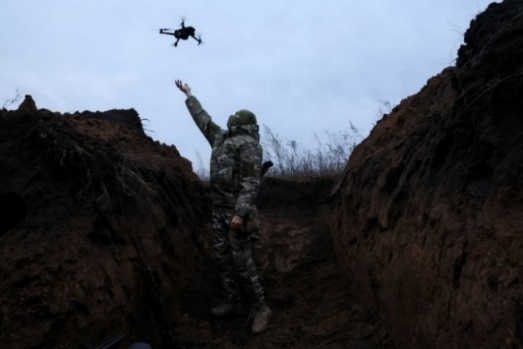
\includegraphics[width=0.8\textwidth]{assets/10}
	\caption*{}
\end{figure}\begin{figure}[H]
	\centering
	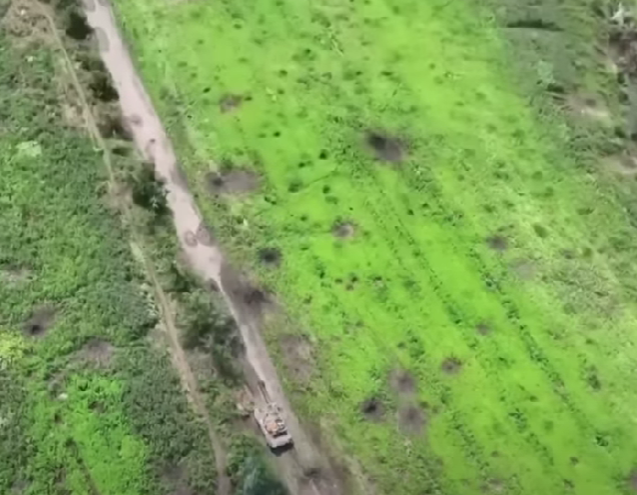
\includegraphics[width=0.8\textwidth]{assets/11}
	\caption*{}
\end{figure}

a)

\begin{enumerate}
\def\labelenumi{\alph{enumi})}
\item
  b)
\end{enumerate}

\textbf{Figure 1- Drone in battlefield. a) Drone take off for
reconnaissance b) Information received during reconnaissance}

cannot be overstated, especially in the context of modern warfare, where
precision and accuracy are paramount. This aspect of military operations
has gained even greater importance with the advent of drones. In
contemporary combat scenarios, the ability to accurately identify and
track targets is crucial for several reasons. It enhances operational
efficiency by enabling precise and timely decision-making {[}2{]}. Armed
with accurate information on the location and nature of a target,
military strategists can devise more effective tactics, allocate
resources more judiciously, and achieve objectives with greater
precision. This is particularly vital in asymmetric warfare and
counterterrorism operations, where identifying the correct targets while
avoiding civilian casualties is both a moral imperative and a strategic
necessity. Advanced target identification and tracking systems
integrated into drone technology greatly improve situational awareness.
Drones equipped with cutting-edge sensors and cameras can relay
real-time information, providing commanders with a comprehensive view of
the battlefield. This capability is invaluable in complex environments,
where visibility is limited, and threats can emerge from any direction.
By maintaining constant surveillance and tracking movements, drones
contribute to a more informed and responsive command structure.

\textbf{Literature Review.} The realm of military operations has
significantly advanced with the integration of various technological
methods for target identification and tracking. One of the methods
related with hyperspectral imagery.

Key among these are approaches utilizing hyperspectral imagery, advanced
neural networks, and high-resolution imaging techniques. A notable
advancement is the use of Hyperspectral Imagery for the detection of
military vehicles. This technology offers detailed spectral
characteristics of targets, which, when processed through techniques
like Principal Component Analysis and k-means clustering, results in the
generation of superpixels. These superpixels enhance the ability to
identify specific military objectives, providing a significant edge in
vehicle detection {[}3{]}. Object detection faces unique challenges,
including dealing with camouflage, blur, inter-class similarity,
intra-class variance, and complex environmental conditions. Addressing
these issues, the MOD benchmark proposes the use of LGA-RCNN. This model
employs loss-guided attention to improve detection performance in these
challenging scenarios {[}4{]}. Another innovative approach involves the
deployment of Convolutional Neural Networks on embedded platforms like
the TMS320C6678. This method showcases a fine balance between
performance and resource constraints, contributing significantly to the
accuracy and efficiency of military operations {[}5{]}. Alternative
method of object tracking it's use YOLO5 architecture marks a leap in
identifying and detecting small, camouflaged military objects. This
model greatly improves the clarity and detail of images, thus aiding in
more accurate object detection, a critical factor in modern military
operations {[}6{]}. After thorough analysis of available literature, we
have opted to employ the YOLO and Deepsort algorithms for our tracking
and target identification endeavor. These algorithms demonstrate
promising capabilities in accurately detecting and tracking objects in
real-time scenarios. With their robust features and proven performance,
we believe they are well-suited for fulfilling the requirements of our
task efficiently and effectively.

\textbf{Main Provision.} The primary goal of this research is to develop
a highly efficient, accurate, and robust system for target
identification and tracking in complex environments, leveraging the
integration of YOLO and Deep Sort. This study is anchored in the
hypothesis that the combination of YOLO rapid detection capabilities
with Deep Sort detailed feature analysis will significantly enhance
object recognition accuracy and operational efficiency, particularly in
challenging conditions.

\begin{figure}[H]
	\centering
	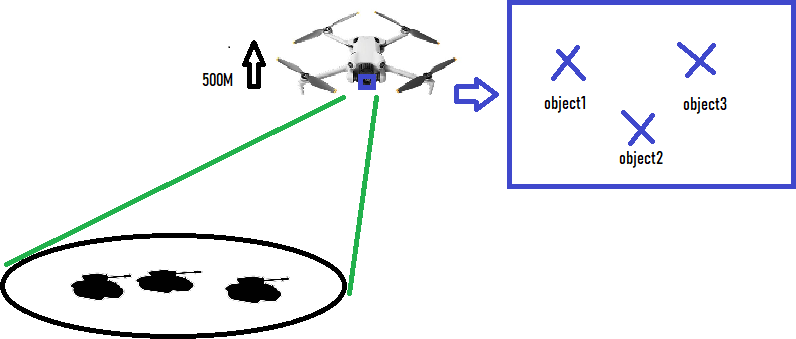
\includegraphics[width=0.8\textwidth]{assets/12}
	\caption*{}
\end{figure}The
drone is shown flying at an altitude of 500 meters above the ground. The
drone is equipped with a sensor or camera (indicated by the blue square
on the drone), which is used to observe objects on the ground. The green
lines from the drone to the ground suggest that the
drone\textquotesingle s sensors are focused on a specific area on the
ground. This could be the drone\textquotesingle s camera field of view.
On the ground, there are three black shapes that appear to be the
objects of interest---perhaps these are the targets the drone is meant
to observe or monitor. The arrow pointing from the drone to the right
implies that the drone is transmitting data. The box on the right side
of the image shows the process of identifying and classifying the
objects observed by the drone. This could be a visual representation of
the data on a screen for an operator, or it could represent the process
of the onboard computer classifying the objects in real-time. The
objects are labeled as "object1", "object2", and "object3" {[}7{]}.

\textbf{Figure 2- Schematic diagram of drone operation}

\textbf{Methods and Materials.} This section delves into the technical
details of how data annotated, how these algorithms are employed and
fused to achieve superior target recognition accuracy and reliability in
challenging battlefield scenarios. Our approach centered around the
sophisticated integration of two powerful machine learning algorithms:
YOLO and Deep Sort.

In the data collection and preprocessing phase, the process extends
beyond simple acquisition of datasets. We focus on amassing data that
represent a broad spectrum of conditions: differing light settings,
varying weather conditions like rain, fog, and extreme brightness, and a
multitude of angles and distances. This variety ensures that the model
is not only exposed to a wide range of scenarios {[}8{]} but is also
robust enough to handle real-world complexities. Once the data is
collected, the preprocessing phase begins. It is critical to ensure the
data\textquotesingle s integrity and relevance. Cleaning involves
removing any irrelevant or misleading information, which could skew the
model\textquotesingle s learning process {[}9{]}. We employ
sophisticated techniques to filter out noise and irrelevant data,
ensuring that only pertinent and high-quality data feeds into the
training process. Labeling, a crucial step, involves annotating the
datasets with accurate and detailed tags. This process is meticulously
carried out by experts who identify and mark objects within each image
or video frame, ensuring that the model learns from accurate
information. This step is particularly challenging in complex
environments, where objects might be partially obscured or camouflaged.

\begin{figure}[H]
	\centering
	
\includegraphics[width=0.8\textwidth]{assets/13}
	\caption*{}
\end{figure}\begin{figure}[H]
	\centering
	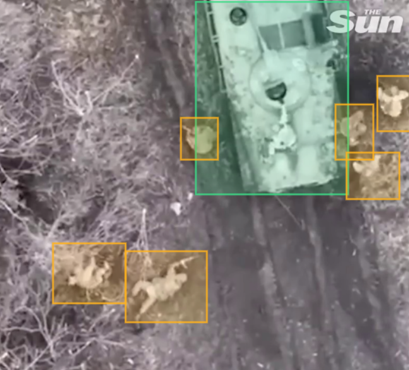
\includegraphics[width=0.8\textwidth]{assets/14}
	\caption*{}
\end{figure}

\textbf{Figure 3 - Data annotation process}

\begin{figure}[H]
	\centering
	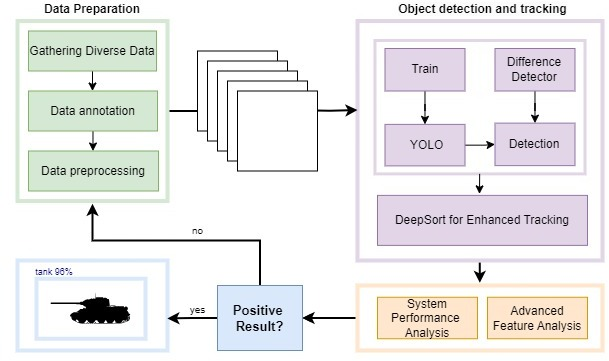
\includegraphics[width=0.8\textwidth]{assets/15}
	\caption*{}
\end{figure}

\textbf{Figure 4 - Flowchart of Machine Learning Process for Object
Detection and Tracking}

YOLO is a state-of-the-art, real-time object detection system that
differs significantly from traditional methods. Traditional object
detection systems repurpose classifiers to perform detection. They apply
the classifier to various locations and scales in an image {[}10{]}.
YOLO, however, applies a single neural network to the full image
{[}11{]}. This network divides the image into regions and predicts
bounding boxes and probabilities for each region. These bounding boxes
are weighted by the predicted probabilities {[}12{]}.

Deep Sort is employed for its superior capabilities in detailed feature
extraction and classification. This algorithm takes the initially
identified objects from YOLO and performs a comprehensive analysis to
classify them accurately. Deep Sort utilizes a convolutional neural
network to extract high-level features from the input images {[}13{]}.
These features are then passed through advanced classification layers
designed to identify subtle and complex features specific to the target
objects. To enhance the model\textquotesingle s ability to generalize,
data augmentation techniques are employed. This includes rotating,
scaling, and flipping images to simulate various viewing conditions.
Deep Sort is trained on a vast dataset of labeled images, which include
various objects in different environmental conditions, ensuring
comprehensive learning {[}14{]}.

\begin{figure}[H]
	\centering
	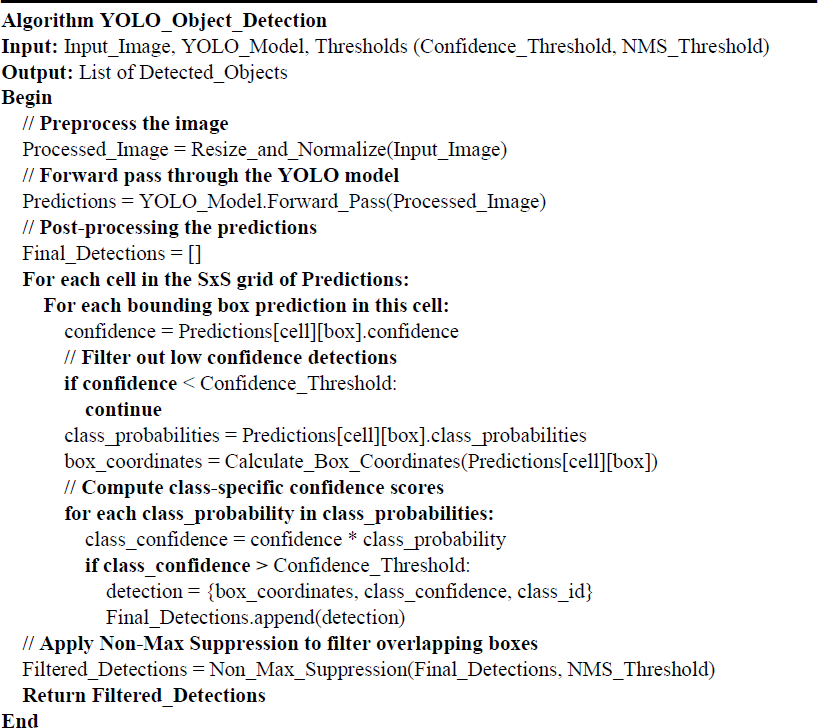
\includegraphics[width=0.8\textwidth]{assets/16}
	\caption*{}
\end{figure}

The integration of YOLO and Deep Sort is the linchpin of our
methodology. The process is not just about running one algorithm after
the other but about creating a seamless, efficient pipeline where the
output of one feeds into the input of the other, optimizing both speed
and accuracy. YOLO rapidly processes the input image to identify
potential targets and their locations. The identified regions by YOLO,
along with their bounding box coordinates, are passed to Deep Sort. Sort
conducts an in-depth analysis of these targeted regions, using its
advanced feature extraction and classification mechanisms. The final
output is a synthesis of both algorithms, where YOLO provides the speed
and initial detection, and Deep Sort offers the depth of analysis and
accuracy in classification {[}15{]}.

\textbf{Results and Discussion.} The integrated YOLO-Deep Sort model
demonstrated exceptional performance in target identification and
tracking. The YOLO algorithm, with its swift real-time object detection
capabilities, successfully identified potential targets within various
complex environments. This initial detection was crucial for setting the
stage for more detailed analysis. Deep Sort's role in providing detailed
feature extraction and classification was evident in the improved
accuracy of target identification. In scenarios with limited visibility
or in the presence of camouflaged objects, Deep Sort was able to discern
and classify the objects with high precision. Our tests showed that the
integration of YOLO and Deep Sort led to a significant reduction in
false positives and negatives compared to when each algorithm was used
independently. In terms of processing speed, the integrated system
maintained a high level of performance, making it viable for real-time
applications in dynamic battlefield environments.

\begin{figure}[H]
	\centering
	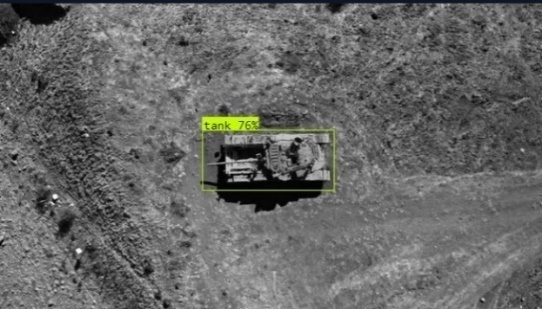
\includegraphics[width=0.8\textwidth]{assets/17}
	\caption*{}
\end{figure}\begin{figure}[H]
	\centering
	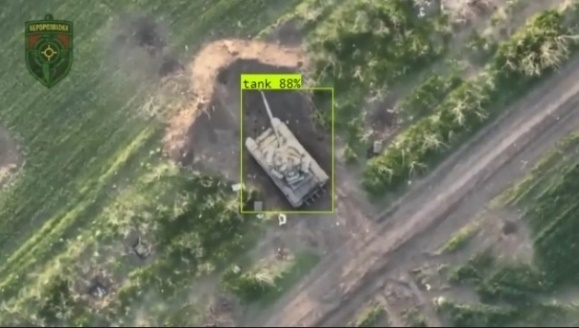
\includegraphics[width=0.8\textwidth]{assets/18}
	\caption*{}
\end{figure}

\textbf{Figure 5 - Object identification}

\begin{figure}[H]
	\centering
	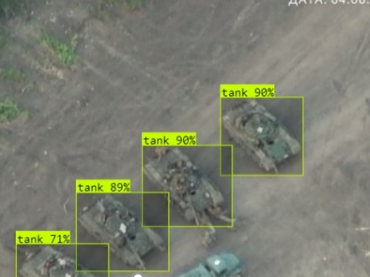
\includegraphics[width=0.8\textwidth]{assets/19}
	\caption*{}
\end{figure}

\begin{figure}[H]
	\centering
	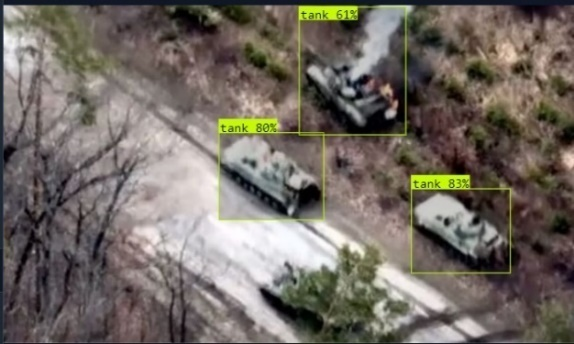
\includegraphics[width=0.8\textwidth]{assets/20}
	\caption*{}
\end{figure}

\textbf{Figure 6 - Multiple object identification}

The model was subjected to rigorous testing in diverse weather
conditions including rain, fog, and extreme brightness. The results were
promising, demonstrating the model\textquotesingle s robustness and
reliability under challenging natural conditions. In urban environments
and rugged terrains, the system maintained a high level of accuracy,
reinforcing its potential for various military applications. The
significance of this work lies in its potential to revolutionize target
identification in complex environments.

\begin{figure}[H]
	\centering
	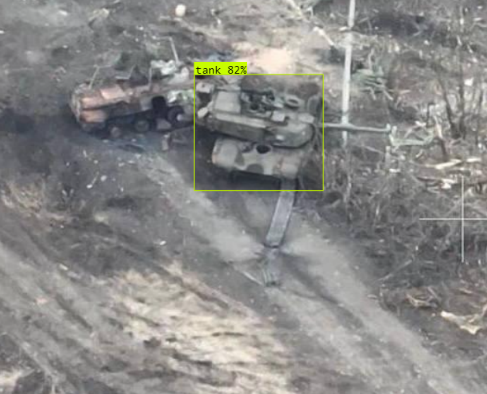
\includegraphics[width=0.8\textwidth]{assets/21}
	\caption*{}
\end{figure}\begin{figure}[H]
	\centering
	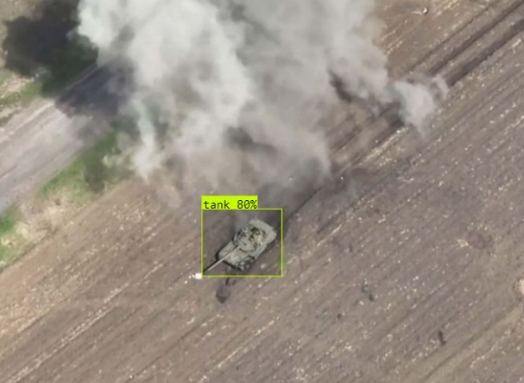
\includegraphics[width=0.8\textwidth]{assets/22}
	\caption*{}
\end{figure}

\textbf{Figure 7 - Complex environment object detection}

\begin{figure}[H]
	\centering
	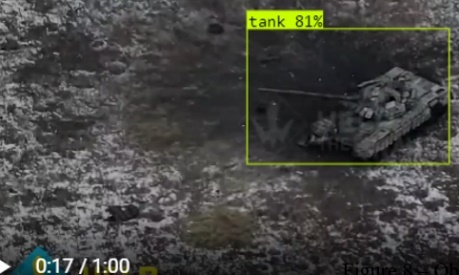
\includegraphics[width=0.8\textwidth]{assets/23}
	\caption*{}
\end{figure}\begin{figure}[H]
	\centering
	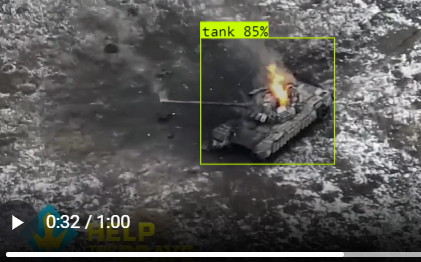
\includegraphics[width=0.8\textwidth]{assets/24}
	\caption*{}
\end{figure}\begin{figure}[H]
	\centering
	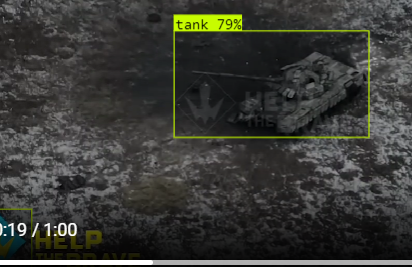
\includegraphics[width=0.8\textwidth]{assets/25}
	\caption*{}
\end{figure}

\textbf{Figure 8 - Object Tracking}

The integrated YOLO-Deep Sort model represents a significant advancement
in the field of military reconnaissance and intelligence gathering. Its
ability to rapidly and accurately identify and track targets in complex
environments provides a substantial strategic advantage. This technology
can enhance situational awareness, enabling more informed
decision-making and effective mission planning. While the model has
shown great promise, there are areas for improvement. One limitation is
the model\textquotesingle s dependency on the quality of input data.
Future work could focus on enhancing the model\textquotesingle s
performance with lower-quality inputs or in scenarios with extreme
environmental conditions. Additionally, further research into reducing
the model\textquotesingle s computational requirements could broaden its
applicability, especially in resource-constrained environments. The
technology has potential applications beyond military operations, such
as in disaster management, where rapid and accurate identification of
objects can aid in effective rescue operations. It can also be adapted
for wildlife monitoring and management, where identifying and tracking
animals in complex environments is crucial. As with any advanced
technology, especially in military applications, ethical considerations
must be addressed. The potential for misuse and the implications of
autonomous target identification systems raise important questions that
need to be carefully considered and regulated.

\textbf{Table 1 -- Object Detection Accuracy Table by Environment Field}

\begin{longtable}[]{@{}
  >{\raggedright\arraybackslash}p{(\columnwidth - 6\tabcolsep) * \real{0.2537}}
  >{\raggedright\arraybackslash}p{(\columnwidth - 6\tabcolsep) * \real{0.2537}}
  >{\raggedright\arraybackslash}p{(\columnwidth - 6\tabcolsep) * \real{0.2537}}
  >{\raggedright\arraybackslash}p{(\columnwidth - 6\tabcolsep) * \real{0.2390}}@{}}
\toprule\noalign{}
\begin{minipage}[b]{\linewidth}\raggedright
\textbf{Environment Field}
\end{minipage} & \begin{minipage}[b]{\linewidth}\raggedright
\textbf{Objects Detected}
\end{minipage} & \begin{minipage}[b]{\linewidth}\raggedright
\textbf{Correct Identifications}
\end{minipage} & \begin{minipage}[b]{\linewidth}\raggedright
\textbf{Detection Accuracy (\%)}
\end{minipage} \\
\midrule\noalign{}
\endhead
\bottomrule\noalign{}
\endlastfoot
Steppe & 1571 & 1509 & 96.1 \\
Forested Terrains & 250 & 239 & 95.6 \\
Desert & 145 & 134 & 92.4 \\
Mountainous Regions & 104 & 91 & 87.5 \\
\end{longtable}

Table presents data on the performance of target identification in
various complex environments. This table effectively conveys how the
complexity of different environments impacts the effectiveness of target
identification technology, with varying degrees of detection accuracy
observed across different terrains.

\textbf{Conclusion.} In conclusion, this research represents a
significant advancement in the field of target identification and
tracking in complex environments using the integration of advanced
machine learning algorithms, YOLO and Deep Sort. This research addresses
the critical challenge of efficient and accurate target detection in
modern military operations, where the use of drones and sophisticated
surveillance techniques is paramount. An integrated approach involving
extensive data collection in a variety of environments and rigorous
preprocessing ensures the adaptability and robustness of the model. The
effectiveness of the integrated system is demonstrated by its ability to
reduce false and negative alarms, maintain high data processing speeds,
and demonstrate resilience to adverse weather conditions and challenging
terrain. Such capabilities are important not only for military
intelligence and intelligence gathering, but also for applications in
disaster management, wildlife monitoring, and other areas where fast and
accurate object identification is important. The study also identifies
areas for future improvement, such as improving model performance when
using lower-quality raw data and reducing computational requirements for
broader applications.

\textbf{References}

1.Jemal R. Brinson, Juanje Gómez, Daniel Michaels, Stephen Kalin. Drones
Are Changing How Wars Are Fought// The wall street Journal.-
2024.https://www.wsj.com/world/drones-are-changing-the-way-wars-are-fought-b6cb4c46

2.Zaher A. (2023). Drones and their Role in the Evolution of Generations
of War. //The International and Political Journal.- 2023.- Vol.56.-
P.69-86. https://doi.org/10.31272/ipj.i56.246. 3.Ke C. Military object
detection using multiple information extracted from hyperspectral
imagery// 2017 International Conference on Progress in Informatics and
Computing (PIC)/-P. 124-128. https://doi.org/10.1109/PIC.2017.8359527.

4.Yi X., Wu J., Ma B., Ou Y., \& Liu L. (2021). MOD: Benchmark for
Military Object Detection. ArXiv, abs/2104.13763.

5.Zeng G., Song R., Hu X., ChenY., \& Zhou X. Applying Convolutional
Neural Network for Military Object Detection on Embedded Platform.
//22nd CCF Conference, NCCET 2018. In book: Communications in Computer
and Information Science- 2018.- P.131-141,

https://doi.org/10.1007/978-981-13-5919-4\_13.

6.Ali S., A.Athar, A.Ali, M.Hussain, A., \& Kim H.Computer Vision-Based
Military Tank Recognition Using Object Detection Technique: An
application of the YOLO Framework.// 2023 1st International Conference
on Advanced Innovations in Smart Cities (ICAISC).-P. 1-6.
https://doi.org/10.1109/ICAISC56366.2023.10085552.

7.Zhang, Z. Based on YOLO v3 Target Recognition Algorithm as Vehicle
Tracking Algorithm Analysis.// Frontiers in Computing and Intelligent
Systems.- 2023.-Vol.5(2).- P.140-144
https://doi.org/10.54097/fcis.v5i2.13146.~

8.Qu J., \& Zhang S. Research on Video Tracking Algorithm Based on Yolo
Target Detection.// 2023 6th International Conference on Computer
Network, Electronic and Automation (ICCNEA).-P. 437-439.
https://doi.org/10.1109/ICCNEA60107.2023.00098.

9.Jiao L., Zhang F., Liu F., Yang, S., Li L., Feng Z., \& Qu, R. A
Survey of Deep Learning-Based Object Detection.//
IEEEAccess.-2019.-Vol.7.- P.128837-128868

https://doi.org/10.1109/ACCESS.2019.2939201.

10.Grebo, A., Konsa, T., Gašparović, G., \& Klarin, B. (2020).
Application of YOLO algorithm on student UAV.// 2020 5th International
Conference on Smart and Sustainable Technologies (SpliTech).-P. 1-6.
https://doi.org/10.23919/SpliTech49282.2020.9243691.

11.Gao B. Research on Two-Way Detection of YOLO V5s+Deep Sort Road
Vehicles Based on Attention Mechanism.// Journal of Physics: Conference
Series.-2022.- Vol.2303.
https://doi.org/10.1088/1742-6596/2303/1/012057.

12.Yan, F., \& Xu, Y. (2021). Improved Target Detection Algorithm Based
on YOLO.// 2021 4th International Conference on Robotics, Control and
Automation Engineering (RCAE).- P.21-25.
https://doi.org/10.1109/RCAE53607.2021.9638930.

13.Hou X., Wang Y. \& Chau L. Vehicle Tracking Using Deep SORT with Low
Confidence Track Filtering. //2019 16th IEEE International Conference on
Advanced Video and Signal Based Surveillance (AVSS).-P. 1-6.
https://doi.org/10.1109/AVSS.2019.8909903.

14.Meimetis, D., Daramouskas, I., Perikos, I., \& Hatzilygeroudis, I.
(2021). Real-time multiple object tracking using deep learning methods.
//Neural Computing and Applications.-2021.-Vol. 35(1).-P. 89-118.
https://doi.org/10.1007/s00521-021-06391-y.

15.Belmouhcine A., Simon J., Courtrai L. \& Lefèvre S. Robust Deep
Simple Online Real-Time Tracking.// 2021 12th International Symposium on
Image and Signal Processing and Analysis (ISPA).-P 138-144.
https://doi.org/10.1109/ISPA52656.2021.9552062

\emph{\textbf{Information about the authors}}

Karim A.- Kazakh-British Technical University, Bachelor, Almaty,
Kazakhstan, ORCID ID: 0009-0008-7355-2099, e-mail: ad\_karim@kbtu.kz;

Muhammad I.- Kazakh-British Technical University, PhD, Professor,
Almaty, Kazakhstan,ORCID ID: 0000-0001-7555-3839, e-mail:
m.ilyas@kbtu.kz

\emph{\textbf{Сведение об авторах}}

Карим А. -Казахский-Британский Технический Университет, бакалавр,
Алматы, Казахстан, ORCID ID: 0009-0008-7355-2099, e-mail:
ad\_karim@kbtu.kz;

Мухаммад И.- Казахский-Британский Технический Университет,PhD,
профессор, Алматы, Казахстан, ORCID ID: 0000-0001-7555-3839, e-mail:
m.ilyas@kbtu.kz

\textbf{ҒТАМР 20.15.05}

\begin{quote}
\textbf{ЖЕЛІ ҚАУІПСІЗДІГІН ҚАМТАМАСЫЗ ЕТУДЕ ТРАФИКТІ ТАЛДАУ ҚҰРАЛДАРЫН}

\textbf{ҚОЛДАНУ АРҚЫЛЫ АУЫТҚУЛАР МЕН ЫҚТИМАЛ ҚАУІПТЕРДІ АНЫҚТАУ}

\textbf{Ж. Бидахмет, А. Уайда, Р.Е.Әлішер, Д. Бағдаулет, Қ. Қаржаубаев
,}

\textbf{А.Сердалы, Ә. Ахметов}

әл-Фараби атындағы Қазақ ұлттық университеті, Алматы, Қазақстан,

е-mail: uaida\_a@mail.ru
\end{quote}

Мақалада компьютерлік желілерде ақпарат жинау әдістері және олардың
қазіргі цифрлық қоғамдағы желілік қауіпсіздікті қамтамасыз етудегі
маңызы қарастырылады, яғни компьютерлік желілердегі ақпаратты түсіру
құралдарының желілік қауіпсіздігі талданады. Қазіргі ақпараттық қоғамда
бұл құралдардың маңызы артып келеді. Трафикті талдау процесі желі арқылы
берілетін деректерді бақылау, жазу және талдау арқылы ауытқулар мен
ықтимал қауіптерді анықтауды қамтиды. Мақалада Wireshark, Tcpdump және
Macof сияқты құралдардың функционалдығы мен қолдану әдістері тереңірек
қарастырылған. Осы құралдарды қолдану әдістері талқыланып, олардың
әрқайсысының ерекшеліктері мен мүмкіндіктері көрсетілген. Әртүрлі
желілік құралдарды тиімді пайдалану арқылы желідегі қауіп-қатерлерді
алдын-ала анықтау және жою мүмкіндігіне баса назар аударылды. Бұл
құралдардың көмегімен желілік қауіпсіздік деңгейін арттыруға, желі
ақауларын жылдам табуға және жоюға болатыны көрсетілген. Сонымен қатар,
мақалада әрбір құралдың артықшылықтары мен кемшіліктерін салыстыра
отырып, олардың қай жағдайда тиімді екені анықталды.

\textbf{Түйін сөздер:} ақпарат, желі, қауіпсіздік, трафик, Wireshark,
Tcpdump, Macof

\textbf{ВЫЯВЛЕНИЕ ОТКЛОНЕНИЙ И ПОТЕНЦИАЛЬНЫХ УГРОЗ С ПОМОЩЬЮ
ИНСТРУМЕНТОВ АНАЛИЗА ТРАФИКА В ОБЕСПЕЧЕНИИ}

\textbf{БЕЗОПАСНОСТИ СЕТИ}

\begin{quote}
\textbf{Ж. Бидахмет, А. Уайда, Р.Е. Алишер, Д. Багдаулет, К.
Каржаубаев,}

\textbf{А.Сердалы, А. Ахметов}

Казахский национальный университет им. Аль-Фараби, Алматы, Казахстан,

е-mail: uaida\_a@mail.ru
\end{quote}

В статье рассматриваются методы сбора информации в компьютерных сетях и
их значение для обеспечения сетевой безопасности в современном цифровом
обществе, т. е. анализируется сетевая безопасность средств захвата
информации в компьютерных сетях. В современном информационном обществе
значение этих средств возрастает. Процесс анализа трафика включает
выявление аномалий и потенциальных угроз путем мониторинга, записи и
анализа данных, передаваемых по сети. В статье подробно рассматриваются
функциональные возможности и методы использования таких инструментов,
как Wireshark, Tcpdump и Macof. Обсуждаются методы применения этих
средств, демонстрируются особенности и возможности каждого из них. Упор
был сделан на возможность заранее выявлять и устранять угрозы в сети с
помощью эффективного использования различных сетевых инструментов. Было
показано, что с помощью этих инструментов можно повысить уровень сетевой
безопасности, быстро найти и устранить проблемы с сетью. Кроме того, в
статье сравниваются преимущества и недостатки каждого средства, чтобы
определить, в каких случаях они наиболее эффективны.

\textbf{Ключевые слова:} информация, сеть, безопасность, трафик,
Wireshark, Tcpdump, Macof

\textbf{IDENTIFY DEVIATIONS AND POTENTIAL THREATS USING TRAFFIC
ANALYSIS}

\textbf{TOOLS TO ENSURE NETWORK SECURITY}

\textbf{Zh.Bidakhmet, A. Uaida, Alisher R., D. Bagdaulet, K.
Karzhaubaev,}

\textbf{A. Serdaly, A. Akhmetov}

\begin{quote}
Al-Farabi Kazakh National University, Almaty, Kazakhstan,

е-mail: uaida\_a@mail.ru
\end{quote}

The article discusses methods of information capture in computer
networks and their importance for network security in
today\textquotesingle s digital society, i.e. it analyzes the network
security of information capture tools in computer networks. In
today\textquotesingle s information society, the importance of these
tools is increasing. The process of traffic analysis involves
identifying anomalies and potential threats by monitoring, recording and
analyzing data transmitted over the network. The article discusses in
detail the functionality and methods of using tools such as Wireshark,
Tcpdump and Macof. The methods of using these tools are discussed, the
features and capabilities of each of them are demonstrated. The emphasis
was placed on the ability to identify and eliminate threats in the
network in advance through the effective use of various network tools.
It has been shown that using these tools it is possible to increase the
level of network security, quickly find and fix network problems. In
addition, the article compares the advantages and disadvantages of each
remedy to determine in which cases they are most effective.

\textbf{Keywords:} information, network, security, traffic, Wireshark,
Tcpdump, Macof

\textbf{Кіріспе.} Қазіргі ақпараттық қоғамда деректерді тасымалдау
әртүрлі желелік орталарда жүзеге асырылады. Сондықтан деректерді
тасымалдау қауіпсіздігін қамтамасыз ету және құпия ақпаратты қорғау
басты мәселе болып табылады. Бұл контексте негізгі аспектілердің бірі
ақпаратты ұстау құралдарын талдау болып табылады.

Деректерді ұстап алу - бұл желі арқылы берілетін немесе электронды түрде
сақталған деректерді заңсыз немесе рұқсат етілген жинау процесі. Бұл
процесс желілік трафикті бақылауды, хабар мазмұнын талдауды және сақтау
құрылғыларынан деректерді жинауды қамтуы мүмкін {[}1{]}.

Желі қауіпсіздігін қамтамасыз етуде трафикті талдау басты рөл атқарады.
Ол желілік инфрақұрылымға бағытталған ықтимал қауіптерді, ауытқуларды
және шабуылдарды анықтауға мүмкіндік береді. Деректердің тасымалдануын
бақылау және пакеттерді талдау арқылы оқиғаларға тез жауап беруге және
құпия ақпараттың ағып кетуіне жол бермеуге болады {[}2{]}.

Трафикті талдау желілік инфрақұрылымның осалдықтарын анықтауға және
жоюға мүмкіндік береді, оның әртүрлі шабуыл түрлерінен сенімді қорғалуын
қамтамасыз етеді. Бұл процесс сонымен қатар желі өнімділігін жақсарту
мүмкіндіктерін анықтау арқылы желі өнімділігін оңтайландыруға
көмектеседі. Тыңдауды талдау желі қауіпсіздігін қамтамасыз ету және
деректердің құпиялылығын қорғаудың маңызды құралы болып табылады.
Төменде біз осы процестің негізгі аспектілерін, трафикті талдау
әдістерін және осы салада тиімді жұмыс істеу үшін қолданылатын
құралдарды қарастырамыз.

\textbf{Материалдар мен әдістер.} Желілік трафикті талдау құралдары --
компьютерлік желілерде деректердің берілуін бақылауға көмектесетін
бағдарламалар мен утилиталар. Олар желі арқылы өтетін ақпаратты көруге,
талдауға және жазуға мүмкіндік береді. Бұл құралдар желі проблемаларын
анықтауға ғана емес, сонымен қатар деректерді беру қауіпсіздігін
қамтамасыз етуге және желілік трафиктегі ықтимал қауіптер мен
ауытқуларды анықтауға көмектеседі. Бұл мәселелерді тиімді шешу үшін
желілік трафикті талдаудың бірнеше қуатты құралдары бар, олардың
арасында Wireshark, Tcpdump және Macof ерекшеленеді {[}3{]}.

Wireshark -- желі белсенділігін бақылауға, талдауға және жөндеуге
мүмкіндік беретін қуатты желі трафигін талдау құралы. Ол желілік
интерфейс арқылы өтетін деректер пакеттерін ұстап алуға және әрбір пакет
туралы егжей-тегжейлі ақпаратты, соның ішінде протокол тақырыптарын,
деректер мен басқа сипаттамаларды беруге қабілетті.

Wireshark негізгі мүмкіндіктері мен мүмкіндіктеріне мыналар жатады:

\begin{enumerate}
\def\labelenumi{\arabic{enumi}.}
\item
  Қолдау көрсетілетін бірнеше протоколдар: Wireshark 2000-нан астам
  әртүрлі желілік протоколдарды қолдайды, бұл оны әртүрлі желі
  сценарийлерін талдауға арналған әмбебап құрал етеді.
\item
  Графикалық пайдаланушы интерфейсі (GUI): Қарапайым және интуитивті
  интерфейс Wireshark-пен жұмыс істеуді тәжірибелі және жаңадан бастаған
  пайдаланушылар үшін ыңғайлы етеді.
\item
  Сүзу және іздеу: үлкен көлемдегі деректерді өңдеуді жеңілдете отырып,
  тек қажетті ақпаратты бөлектеуге және талдауға мүмкіндік береді.
\end{enumerate}

Wireshark - желі әкімшілері, қауіпсіздік инженерлері, желілік
қосымшаларды әзірлеушілер және желілік инфрақұрылыммен жұмыс істейтін
кез келген басқа адамдар үшін маңызды құрал.

Tcpdump -- желілік трафикті талдауға арналған пәрмен жолы утилитасы. Ол
компьютердің желілік интерфейсі арқылы өтетін деректер пакеттерін
ұстауға және көрсетуге мүмкіндік береді. Tcpdump бағдарламасының маңызды
ерекшелігі оның нақты уақыт режимінде жұмыс істеу мүмкіндігі болып
табылады, бұл оны желі мәселелерін диагностикалау және талдау үшін
қуатты құрал етеді {[}4{]}.

Tcpdump негізгі мүмкіндіктері мен функцияларына мыналар жатады:

\begin{enumerate}
\def\labelenumi{\arabic{enumi}.}
\item
  Көп протоколды қолдау: Tcpdump TCP, UDP, ICMP және т.б. сияқты әртүрлі
  желілік протоколдарды пайдаланып пакеттерді талдауға қабілетті.
\item
  Трафикті сүзу: пайдаланушыға тек белгілі бір пакеттерді (мысалы,
  дереккөз, тағайындалған орын, порт және басқа параметрлер бойынша)
  көрсету үшін нақты критерийлерді көрсетуге мүмкіндік береді.
\item
  Файлдарды оқу және жазуды қолдау: Tcpdump желі трафигінің сақталған
  файлдарымен жұмыс істей алады, сонымен қатар кейінірек талдау үшін
  файлға ағымдағы трафикті жаза алады.
\end{enumerate}

Tcpdump -- желі әкімшілері, қауіпсіздік инженерлері және желілік
трафикті талдаумен жұмыс істейтін кез келген адам үшін маңызды құрал.

Macof - бұл кездейсоқ MAC мекенжайларының үлкен санын жасауға және
оларды желіге жіберуге арналған пәрмен жолы құралы. Macof
бағдарламасының негізгі мақсаты - желі жұмысын баяулату немесе бұзу үшін
жалған MAC мекенжайларының көп санын жасау {[}5{]}.

Macof көмегімен жалған MAC мекенжайларын жасау мүмкіндіктері мыналарды
қамтиды:

\begin{enumerate}
\def\labelenumi{\arabic{enumi}.}
\item
  Кездейсоқ генерация: Macof MAC мекенжайларын кездейсоқ түрде жасайды,
  бұл оларды болжауды қиындатады.
\item
  Желіге жіберу: Жасалған MAC мекенжайлары компьютердің желілік
  интерфейсі арқылы желіге жіберіледі.
\item
  Ықтимал шабуылдар: Macof коммутаторлар сияқты желілік құрылғыларды
  шамадан тыс жүктеуге немесе баяулатуға бағытталған шабуылдарда
  қолданылуы мүмкін.
\end{enumerate}

Macof пайдалану сақтықты қажет ететінін ескеру маңызды, себебі бұл
құралды дұрыс пайдаланбау желінің бұзылуына және қажетсіз жүктемеге
әкелуі мүмкін. Ол көбінесе желілік қауіпсіздікті тестілеуде және желіні
оқытуда қолданылады.

\textbf{Нәтижелер мен талқылау.} Wireshark мысалы: Енді біз Wireshark
трафикті ұстау және талдау мүмкіндіктерін көрсетеміз. Wireshark-ты іске
қосып, тізімнен бақылау интерфейсін таңдайық, біздің жағдайда бұл eth0
болады (1-сурет).

Интерфейсті таңдағаннан кейін деректерді жинау басталады. Тараудың
басында біз сымсыз желілердегі трафикті бақылау өте қарапайым екенін
айттық. Міне осылай - сымсыз желідегі барлық компьютерлерден деректерді
көру үшін сізге қажетті интерфейсті таңдау керек.

\begin{longtable}[]{@{}
  >{\raggedright\arraybackslash}p{(\columnwidth - 2\tabcolsep) * \real{0.4984}}
  >{\raggedright\arraybackslash}p{(\columnwidth - 2\tabcolsep) * \real{0.5016}}@{}}
\toprule\noalign{}
\begin{minipage}[b]{\linewidth}\raggedright
% \begin{figure}[H]
% 	\centering
% 	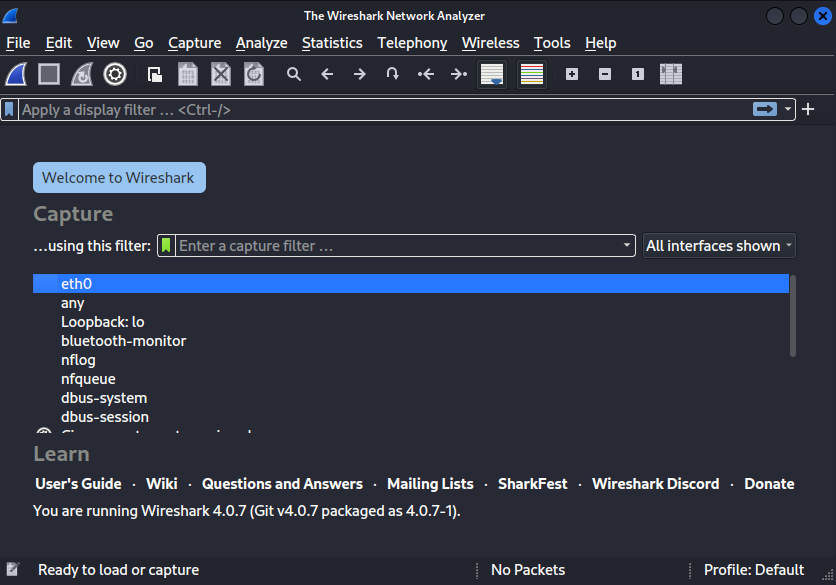
\includegraphics[width=0.8\textwidth]{assets/26}
% 	\caption*{}
% \end{figure}

\textbf{1-сурет - Интерфейсті таңдау}
\end{minipage} & \begin{minipage}[b]{\linewidth}\raggedright
% \begin{figure}[H]
% 	\centering
% 	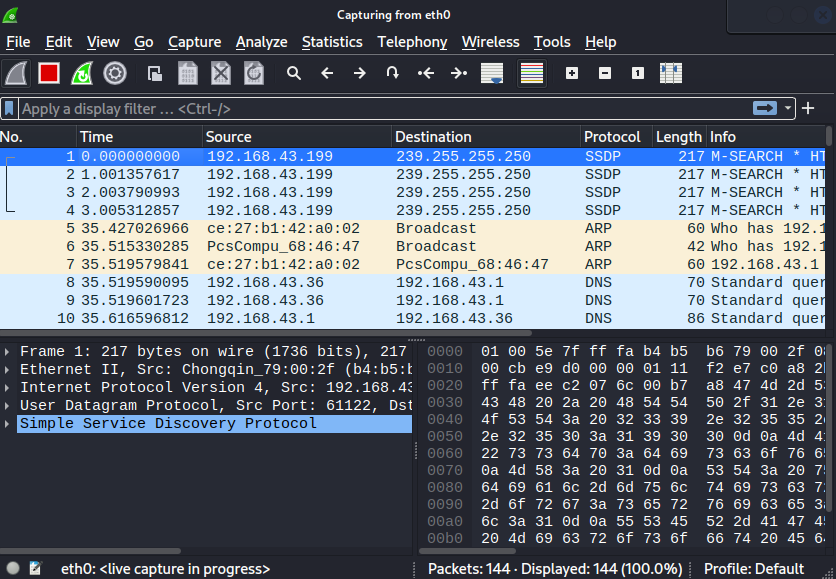
\includegraphics[width=0.8\textwidth]{assets/27}
% 	\caption*{}
% \end{figure}

\textbf{2-сурет -Жиналған пакеттер}
\end{minipage} \\
\midrule\noalign{}
\endhead
\bottomrule\noalign{}
\endlastfoot
\end{longtable}

Қажетті деректер көлемін жинағаннан кейін пакеттерді жинауды тоқтатыңыз
(2-сурет). Енді оларды кейінірек талдау үшін сақтауға немесе оны бірден
бастауға болады. Бірнеше минут ішінде біз 20 000-ға жуық пакет жинадық,
бұл желідегі трафик аз болған жағдайда болды. Әрине, мұндай пакеттерді
қолмен қарау өте көп еңбекті қажет ететін жұмыс және оны жеңілдету үшін
Wireshark әртүрлі сүзгілерді ұсынады (1-кесте).

\textbf{1-кесте - Wireshark сүзгілері}

\begin{longtable}[]{@{}
  >{\raggedright\arraybackslash}p{(\columnwidth - 4\tabcolsep) * \real{0.3333}}
  >{\raggedright\arraybackslash}p{(\columnwidth - 4\tabcolsep) * \real{0.3333}}
  >{\raggedright\arraybackslash}p{(\columnwidth - 4\tabcolsep) * \real{0.3334}}@{}}
\toprule\noalign{}
\begin{minipage}[b]{\linewidth}\raggedright
Оператор
\end{minipage} & \begin{minipage}[b]{\linewidth}\raggedright
Функция
\end{minipage} & \begin{minipage}[b]{\linewidth}\raggedright
Мысал
\end{minipage} \\
\midrule\noalign{}
\endhead
\bottomrule\noalign{}
\endlastfoot
== & Тең & Ip.addr == 192.168.10.12 \\
eq & Тең & Tcp.port eq 80 \\
!= & Тең емес & Ip.addr != 192.168.10.5 \\
ne & Тең емес & Ip.src ne 192.168.10.5 \\
contains & Құрамында & Hhtp contains ``google.com'' \\
\end{longtable}

Google.com веб-сайтына пайдаланушы сұрауларын сүзгіден өткізейік. DNS
сұрауынан бастайық, өйткені ол әрқашан бірінші болады. Сүзгіні қолдану
арқылы біз браузер сұрауларының және DNS серверіне жауаптардың толық,
дәйекті тарихын көреміз. Енді қай IP мекенжайы әрі қарай байланыс
болатынын біле отырып, сәйкес сүзгіні жасайық (ip.addr==192.168.43.36)
(3-сурет).

\begin{figure}[H]
	\centering
	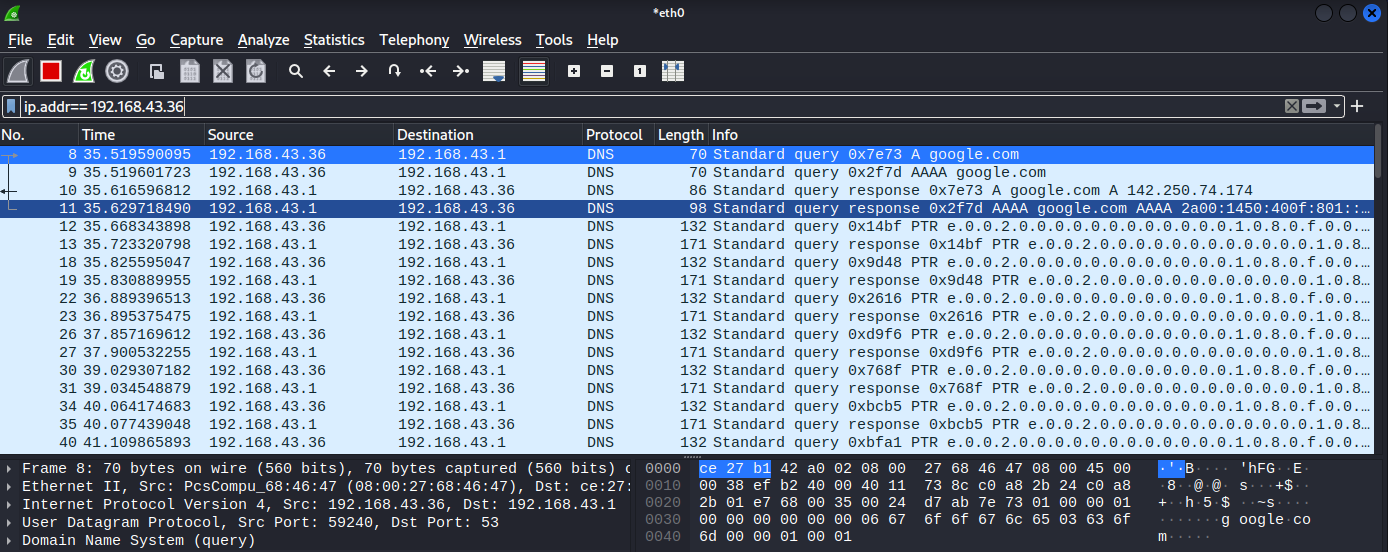
\includegraphics[width=0.8\textwidth]{assets/28}
	\caption*{}
\end{figure}

\textbf{3-сурет- Веб-сервермен байланыс}

Көріп отырғаныңыздай, сүзгіден өткен пакеттердің саны 1153 (3-сурет).
Олардың әрқайсысы деректердің аз ғана бөлігін ғана жібереді және оларда
қандай ақпарат бар екенін түсіну өте қиын. Тапсырманы жеңілдету үшін
Wireshark нақты деректер ағынын бақылаудың керемет мүмкіндігіне ие. UDP
жағдайында «UDP Stream» опциясын таңдаңыз {[}6{]}.

Сонымен, біз байланыстың толық, стандартты бейнесін көрдік - DNS
серверінен сұраныс пен жауап, үш жақты қол алысу және деректерді беруді
инициализациялау. Оның үстіне біз пакеттердің мазмұнын да көрдік
(5-сурет).

\begin{figure}[H]
	\centering
	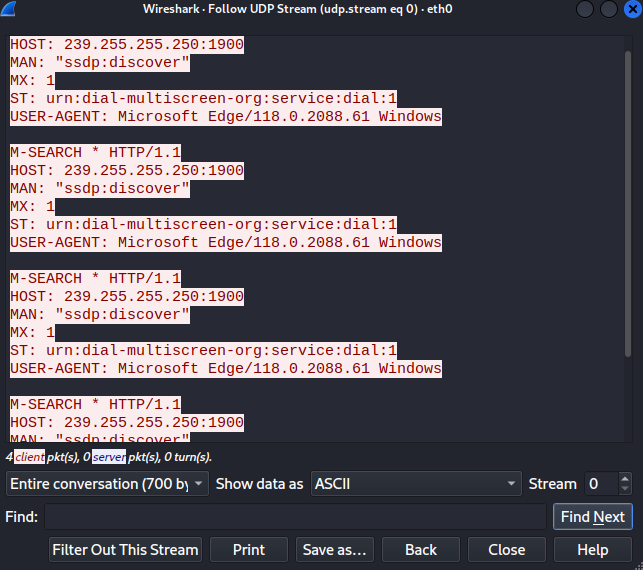
\includegraphics[width=0.8\textwidth]{assets/29}
	\caption*{}
\end{figure}

\textbf{5-сурет- Барлық пайдалы ақпарат бір жерде}

Графикалық интерфейске әрқашан қол жеткізе алмайтыныңызды ескеріңіз,
сондықтан Wireshark алдында пайда болған басқа құрал - tcpdump-пен
танысуды ұсынамыз.

Tcpdump мысалы: Егер сіз жай ғана tcpdump іске қоссаңыз, онда барлық
ақпарат нақты уақыт режимінде шығарылады, бұл кейіннен оны талдау үшін
іс жүзінде жарамсыз етеді (6-сурет).

\begin{figure}[H]
	\centering
	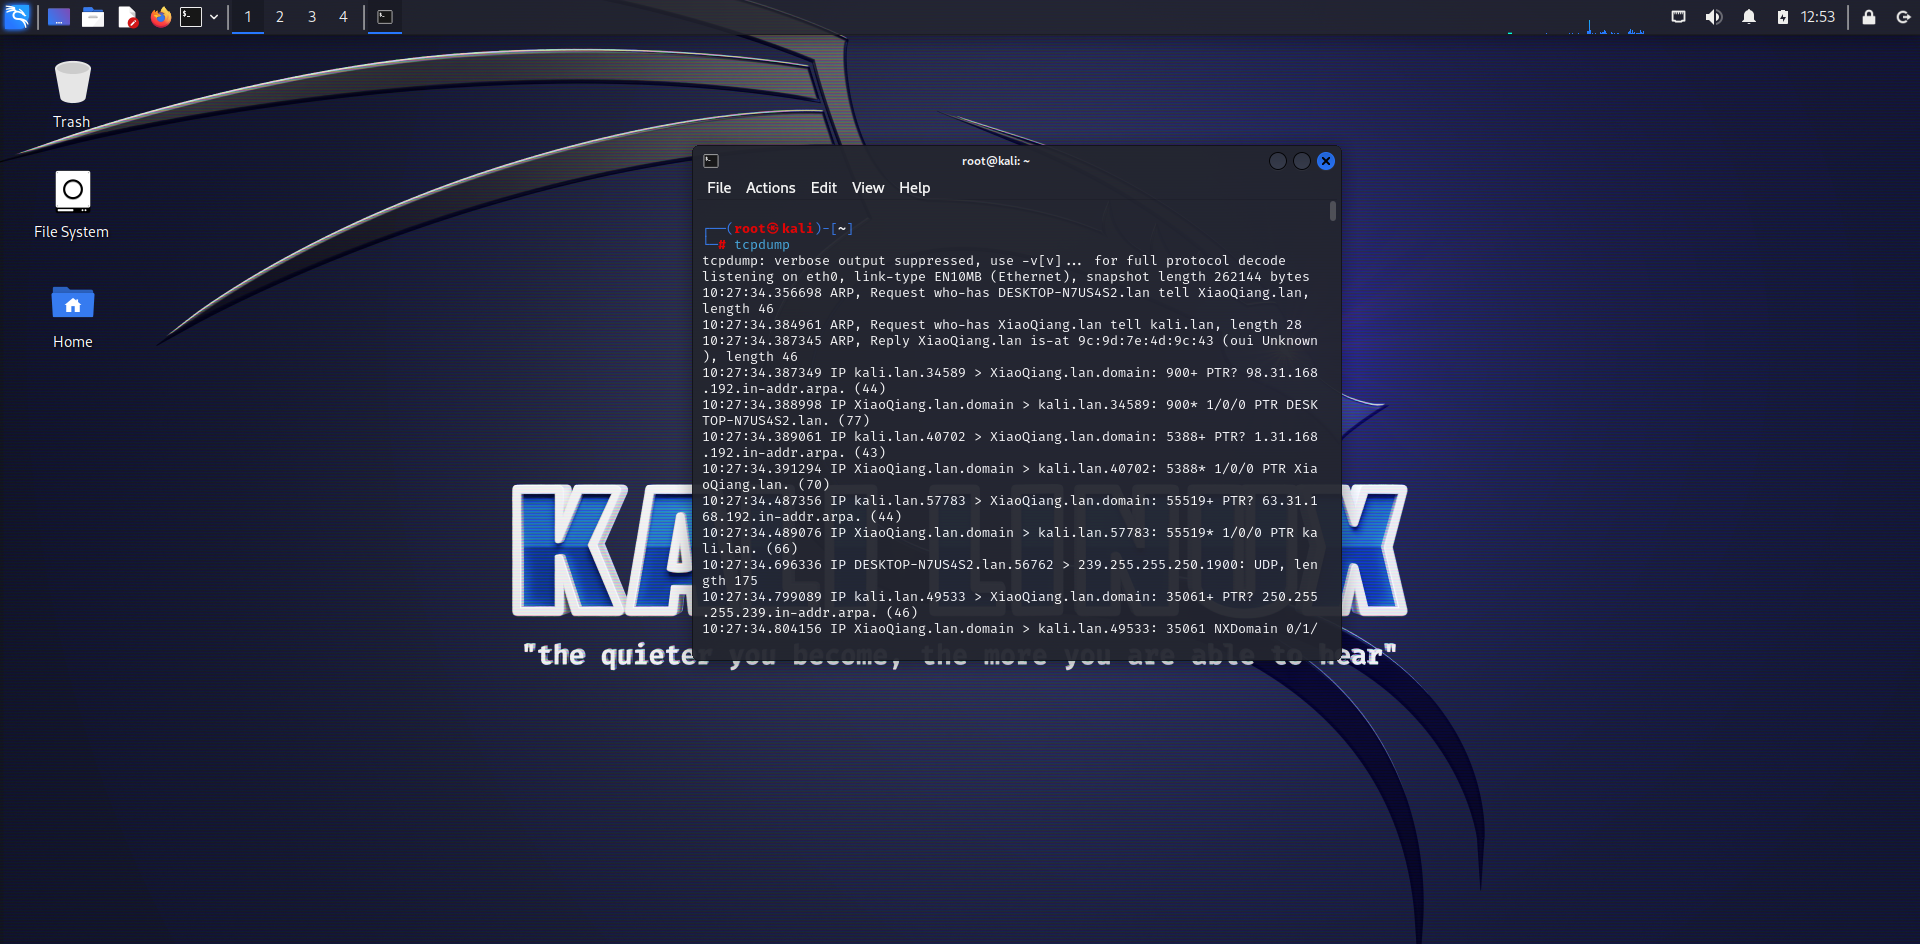
\includegraphics[width=0.8\textwidth]{assets/30}
	\caption*{}
\end{figure}

\textbf{6-сурет -Tcpdump командасының нәтижесі}

Барлық ақпаратты файлға сақтау әлдеқайда жақсы, өйткені бұл деректерді
жинауды жеңілдетеді және сізге ыңғайлы кез келген уақытта кейінгі
трафикті талдау мүмкіндігін жасайды (7-сурет).

\begin{figure}[H]
	\centering
	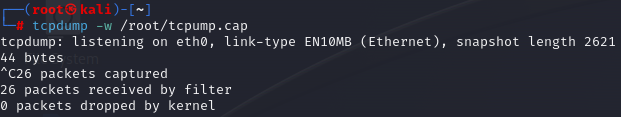
\includegraphics[width=0.8\textwidth]{assets/31}
	\caption*{}
\end{figure}

\textbf{7-сурет- Ақпаратты tcpump.cap парақшасына сақтаймыз}

Алынған деректерді талдау үшін консольді пайдалануға болады. Біз дәйекті
боламыз және консольдегі деректерді талдауға мысал келтіреміз.

Қосылым болған барлық IP мекенжайлары мен порттарын қарастырайық
(8-сурет):

\begin{figure}[H]
	\centering
	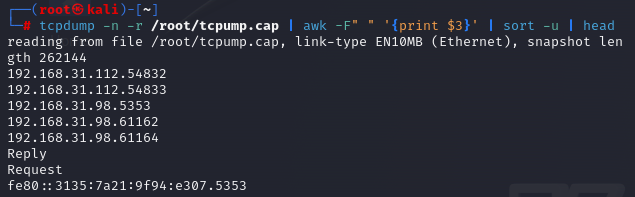
\includegraphics[width=0.8\textwidth]{assets/32}
	\caption*{}
\end{figure}

\textbf{8-сурет- Қосылған IP мекенжайлар тізімі}

Әрі қарай, оны түсіру кезінде желі арқылы жіберілген ақпаратты
қарастырайық. Бұл жағдайда біз оны HEX форматында көреміз, бірақ бұл
бізге қажетті деректерді алуға кедергі болмайды (9-сурет).

\begin{figure}[H]
	\centering
	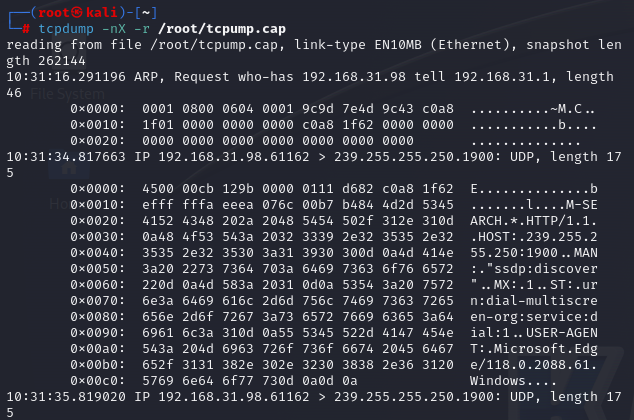
\includegraphics[width=0.8\textwidth]{assets/33}
	\caption*{}
\end{figure}

\textbf{9-сурет -Жіберілген ақпараттар HEX-форматында}

Енді шабуылдаушы коммутатор порттарының біріне қол жеткізе алатын
жағдайды қарастырайық. Бұл жағдайда коммутатордың өзіне қол жеткізу
немесе оның басқа бөлмеде орналасқан желілік жабдыққа қосылған желілік
розетка екендігі маңызды емес. Жалғыз маңызды нәрсе - желілік интерфейс
тек келуі керек пакеттерді қабылдайды, одан артық емес.

Мұндай қорғанысты айналып өтудің және коммутаторды хаб ретінде жұмыс
істеуге мәжбүрлеудің ең танымал тәсілдерінің бірі, бұл бізге барлық
желілік трафикті тоқтатуға мүмкіндік береді, CAM кестесін толтыру болып
табылады {[}7-8{]}.

CAM кестесін MAC мекенжайларымен толтыруға бағытталған шабуылды орындау
үшін бір пәрмен жеткілікті (10-сурет):

\begin{figure}[H]
	\centering
	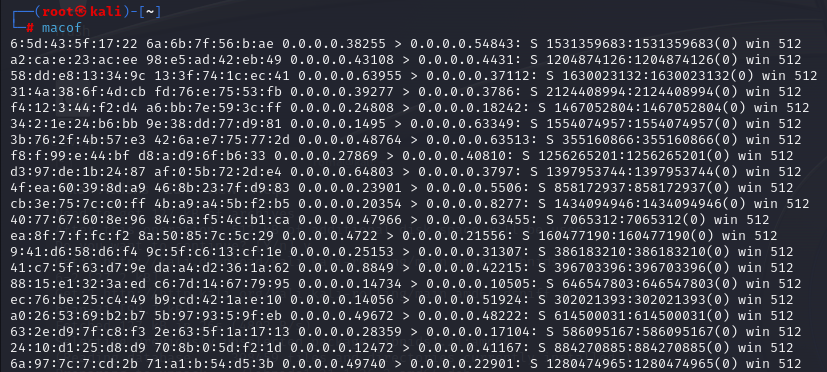
\includegraphics[width=0.8\textwidth]{assets/34}
	\caption*{}
\end{figure}

\textbf{10-сурет - Macof шабуылы}

Тағы бір айта кететін мәселе бар. Егер сіз желілік порттардың біріне қол
жеткізсеңіз де, сіз әлі де желіге кіре алмайсыз, өйткені барлық заманауи
коммутаторлар MAC мекенжайлары бойынша қол жеткізуді басқара алады.
Дегенмен, сізде әрқашан компьютердің MAC мекенжайын келесідей өзгерту
мүмкіндігі бар (11-сурет):

\begin{figure}[H]
	\centering
	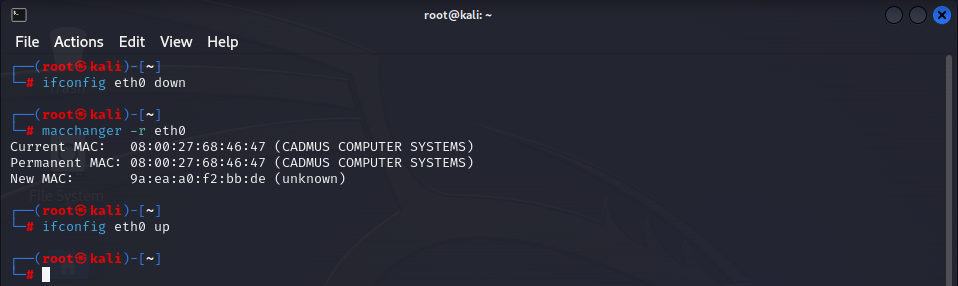
\includegraphics[width=0.8\textwidth]{assets/35}
	\caption*{}
\end{figure}

\textbf{11-сурет- MAC мекенжайына өзгертулер}

Трафик талдауы желі өнімділігі туралы құнды түсінік береді және
қауіпсіздік үшін маңызды болуы мүмкін. Дегенмен, оны өткізу кезінде
этикалық нормаларды сақтауды ұмытпаған жөн. Пайдаланушы деректерінің
құпиялылығы мен құпиялылығын ескеру қажет. Жол қозғалысын талдау
нәтижесінде алынған ақпаратты жинау, талдау және сақтау кезінде
деректерді қорғаудың барлық заңдары мен саясаттарын сақтау ұсынылады.

Деректерді қорғаудың криптографиялық әдістерінің дамуымен шифрланған
трафикті талдау барған сайын қиындай түсуде. Шифрлау пакет мазмұнын
егжей-тегжейлі талдауға елеулі кедергі келтіруі мүмкін. Сарапшылар
шифрланған трафикпен жұмыс істеу дағдыларын дамытуы және шифрланған
байланыстағы қауіптерді анықтай және талдай алатын талдау әдістерін
іздеуі керек {[}9{]}.

Бұл аспектілер трафикті талдаумен жұмыс істеу кезінде аналитиктер
кездесетін шектеулер мен қиындықтарды түсіну үшін маңызды. Осы
факторларды ескере отырып, сарапшылар анағұрлым тиімді талдау
стратегиялары мен әдістерін жасай алады. Технологияның дамуымен және
желілік трафиктің жаңа түрлерінің пайда болуымен оны талдаудың
инновациялық тәсілдерінің қажеттілігі туралы сұрақ туындайды. Желінің
қауіпсіздігі және трафикті талдау саласындағы жетекші сарапшылар
қауіптерді тиімдірек анықтап, талдай алатын жаңа әдістер мен
алгоритмдерді құрумен айналысуда. Трафикті талдау саласында жасанды
интеллект, машиналық оқыту және үлкен деректерді талдауды пайдалану
перспективалы бағыт болып табылады {[}10{]}.

Басқа қауіпсіздік құралдарымен интеграция. Желінің тиімді қауіпсіздігі
кешенді тәсілді қажет етеді. Трафикті талдауды басқа қауіпсіздік
құралдарымен, мысалы, қауіпті бақылау жүйелерімен, шабуылды анықтау
құралдарымен және DDoS қорғау жүйелерімен біріктіру желілік
инфрақұрылымды қорғаудың сенімді және тиімді тетіктерін жасауға
мүмкіндік береді {[}11{]}.

\textbf{Қорытынды.} Зерттеуде желілік трафикті талдаудың негізгі
аспектілері, соның ішінде қолданылатын құралдар, талдау әдістері,
сондай-ақ осы саланың дамуындағы шектеулер мен перспективалар
қарастырылды. Wireshark, Tcpdump және Macof сияқты маңызды құралдардың
мүмкіндіктері мен қолданбалары талқыланды. Желілік трафикті талдаудың
әртүрлі аспектілері, соның ішінде аномалияларды анықтау, желі
өнімділігін бақылау және қауіпсіздік инциденттерін зерттеу әдістері
қарастырылды.

Желілік трафикті талдау құралдарын пайдалану желі қауіпсіздігін
қамтамасыз етудің маңызды элементі болып табылады. Бұл құралдар
аномалияларды анықтап, қауіптерді тауып, желінің жағдайын бақылап,
қауіпсіздік инциденттеріне жауап беруге мүмкіндік береді. Трафикті
талдау арқылы мамандар қауіптерге жылдам жауап беріп, шабуылдардың алдын
алып, желілік инфрақұрылымның үздіксіз жұмысын қамтамасыз етеді.

Желілік трафикті талдау құралдарын пайдалану желінің қауіпсіздік
деңгейін айтарлықтай арттырып, өзгермелі жағдайлар мен қауіптерге жылдам
әрекет етуге мүмкіндік береді. Трафикті талдаудың заманауи әдістерін
әзірлеу және енгізу, оны басқа қауіпсіздік құралдарымен біріктіру және
осы саладағы өзгерістерді үздіксіз бақылау желілік инфрақұрылымның
қауіпсіздігін қамтамасыз етудегі маңызды қадамдар болып табылады.

\textbf{Әдебиеттер}

1.Chris Sanders~Practical Packet Analysis, 3rd Edition: Using Wireshark
to Solve Real-World Network Problems~3rd Edition// No Starch Press.
-2017.- P.120-145, 2017. ISBN: 978-1593278021

2. Chris Sanders,~Jason Smith~ Applied Network Security Monitoring:
Collection, Detection, and Analysis~1st Edition// Syngress.-2013.-
P.200-210. ISBN 978-0124172081.

3.Michael Sikorski,~Andrew Honig~Practical Malware Analysis: The
Hands-On Guide to Dissecting Malicious Software~1st Edition// No Starch
Press.-2012.-P.325. ISBN: 978-1593272906

4. Sherri Davidoff,~Jonathan Ham Network Forensics: Tracking Hackers
through Cyberspace~1st Edition.//Prentice Hall. -2012.-576 P. ISBN
978-0132564717

5. Laura Chappell Wireshark Network Analysis (Second Edition): The
Official Wireshark Certified Network Analyst Study Guide~2nd Revised ed.
Edition// University Laura Chappell.-2012.- P.250-256. ISBN
978-1893939943

6. Richard Stevens TCP/IP Illustrated: The Protocols, Volume 1
(Addison-Wesley Professional Computing Series)~2nd Edition.-2011.-P.
65-75. ISBN: 978-0321336316.

7. William Stallings~Network Security Essentials: Applications and
Standards~6th Edition.-2016.- P.290-302.ISBN: 978-0134527338

8.A. Rahmatulloh, R. Gunawan, and F. M. S. Nursuwars Performance
comparison of signed algorithms on JSON Web Token //in IOP Conference
Series: Materials Science and Engineering.- 2019.- Vol.550(1):012023.
DOI 10.1088/1757-899X/550/1/012023

9. A. Neumann, N. Laranjeiro, J. Bernardino An Analysis of Public REST
Web Service APIs //IEEE Trans Serv Comput.- 2021.- Vol. 14(4).-
P.957-970. DOI 10.1109/TSC.2018.2847344.

10. G. Alonso, F. Casati, H. Kuno, V. Machiraju. Web Services// in Web
Services: Concepts, Architectures and Applications- Eds. Berlin,
Heidelberg: Springer Berlin Heidelberg.- 2004.- P. 123-149. DOI
10.1007/978-3-662-10876-5\_5.

11.\hl{Бидахмет Ж.,Уайда А., Майлыбаева А.Д., Даркенбаев Д.К.,Бекназаров
С.,Бағдаулет Д. Metasploit framework арқылы желі мен сервердегі
осалдықтарды сканерлеу және операциялық жүйелерге қашықтан қол жеткізу.-
Вестник КазУТБ.-2024- № 1(22).- С.97-106}

\emph{\textbf{Авторлар туралы мәліметтер}}

Бидахмет Ж. - PhD, әл-Фараби атындағы Қазақ ұлттық университетінің м.а.
доценті, Алматы, Қазақстан,e-mail:bidakhmetzhanar@gmail.com;

Уайда А. -- әл-Фараби атындағы Қазақ ұлттық университетінің магистранты,
Алматы, Қазақстан, e-mail: uaida\_a@mail.ru;

Бағдаулет Д. - әл-Фараби атындағы Қазақ ұлттық университетінің
магистранты, Алматы, Қазақстан, e-mail: dasik-007@mail.ru;

Әлішер Р. - әл-Фараби атындағы Қазақ ұлттық университетінің магистранты,
Алматы, Қазақстан, e-mail: roma43529@gmail.com;

Қаржаубаев Қ. - әл-Фараби атындағы Қазақ ұлттық университетінің
магистранты, Алматы, Қазақстан, e-mail: Karzhaubayevkuanysh@gmail.com;

Сердалы А.- әл-Фараби атындағы Қазақ ұлттық университетінің магистранты,
Алматы, Қазақстан, e-mail: altynayserdaly@gmail.com;

Ахметов Ә. - әл-Фараби атындағы Қазақ ұлттық университетінің
магистранты, e-mail: Aahmetov755@gmail.com;

\emph{\textbf{Information about authors}}

Bidakhmet Zh.- PhD,Acting Associate Professor NAO Al-Farabi Kazakh
National University, Almaty, Kazakhstan, e-mail:
bidakhmetzhanar@gmail.com;

Uaida A. - graduate student at Al-Farabi Kazakh National University,
Almaty, Kazakhstan, e-mail: uaida\_a@mail.ru;

Bagdaulet D. - graduate student at Al-Farabi Kazakh National University,
Almaty, Kazakhstan, e-mail: dasik-007@mail.ru;

Alisher R. -graduate student of Al-Farabi Kazakh National University,
Almaty, Kazakhstan,e-mail: roma43529@gmail.com;

Karzhaubaev K.- graduate student of Al-Farabi Kazakh National
University, Almaty, Kazakhstan, e-mail: Karzhaubayevkuanysh@gmail.com;

Serdaly A.-graduate student of Al-Farabi Kazakh National University,
Almaty, Kazakhstan, e-mail: altynayserdaly@gmail.com;

Akhmetov A.-graduate student of Al-Farabi Kazakh National University,
Almaty, Kazakhstan,

e-mail:Aahmetov755@gmail.com

IRSTI 50.47.31

\textbf{RESEARCH AND CONSTRUCTION OF A MATHEMATICAL MODEL USING DISCRETE
PROGRAMMING METHODS FOR THE MIXING AND MELTING OF COPPER CONCENTRATES}

\textbf{U. Imanbekova\textsuperscript{1}, A.
Kalizhanova\textsuperscript{2,1}, A.Kozbakova\textsuperscript{2,3}, A.
Imanbekova\textsuperscript{4}, A. Utegenova\textsuperscript{1,2}}

\textsuperscript{1}Almaty University of Power Engineering and
Telecommunications named after G.Daukeyev, Almaty, Kazakhstan,

\textsuperscript{2}Institute of Information and Computational
Technologies CS MSHE RK, Almaty, Kazakhstan,

\textsuperscript{3}Almaty Technological University, Almaty, Kazakhstan,

\textsuperscript{4}Taraz Regional University named after M.Kh. Dulaty,
Taraz, Kazakhstan,

е-mail: uli.08@mail.ru

This paper describes the construction of an optimal schedule for a
metallurgical workshop using discrete programming, and in particular,
the method of branches and boundaries. In this regard, a heuristic
approach to solving this problem is proposed, which includes: building
an initial graph that satisfies the constraints of the optimization
problem, as well as sequential search optimization of the initial graph
according to a given criterion. To test the effectiveness of using the
task of forming a melting schedule as part of the operational control
subsystem in the converter department, experimental studies were
conducted. Considering that the creation of the automated process
control system of the copper plant provides for the introduction of
systems using modern software and hardware controls, cargo flow control,
and an automated conversion process control system, the efficiency of
using optimal melting schedules will significantly increase.

\textbf{Keywords.} Copper raw materials, blending, smelting.

\begin{quote}
\textbf{МЫС КОНЦЕНТРАТТАРЫН ШИХТАУ ЖӘНЕ БАЛҚЫТУ ҮШІН ДИСКРЕТТІ
БАҒДАРЛАМАЛАУ ӘДІСТЕРІМЕН МАТЕМАТИКАЛЫҚ МОДЕЛЬДІ ЗЕРТТЕУ ЖӘНЕ ҚҰРУ}

\textbf{У.Иманбекова\textsuperscript{1},
А.Калижанова\textsuperscript{2,1}, А.Козбакова\textsuperscript{2,3},
А.Иманбекова\textsuperscript{4}, А.Утегенова\textsuperscript{1,2}}
\end{quote}

\textsuperscript{1}Ғ.Дәукеев атындағы Алматы энергетика және байланыс
университеті, Алматы, Қазақстан,

\textsuperscript{2}Ақпараттық және есептеуіш технологиялар институты ҚР
ҒЖБМ ҒК, Алматы, Қазақстан,

\textsuperscript{3}Алматы технологиялық университеті, Алматы, Қазақстан,

\textsuperscript{4}М.Х. Дулати атындағы Тараз өңірлік университеті,
Тараз, Қазақстан,

е-mail: uli.08@mail.ru

Бұл жұмыста дискретті бағдарламалау арқылы, атап айтқанда, бұтақтар мен
шекаралар әдісімен металлургия цехының оңтайлы графигін құру
сипатталған. Осыған байланысты осы мәселені шешуге эвристикалық тәсіл
ұсынылады, оған мыналар кіреді: оңтайландыру мәселесінің шектеулерін
қанағаттандыратын бастапқы графикті құру, сондай-ақ, берілген критерий
бойынша бастапқы графикті дәйекті іздеу жүйесін оңтайландыру.
Конверторлық бөлімшеде жедел басқару кіші жүйесінің құрамымен балқыту
кестесін қалыптастыру міндетін пайдаланудың тиімділігін тексеру үшін
эксперименттік зерттеулер жүргізілді. Мыс зауытының баж ТП құру заманауи
бағдарламалық-техникалық басқару құралдарын, жүк ағынын бақылауды,
айырбастау процесін басқарудың автоматтандырылған жүйесін қолдана отырып
жүйелерді енгізуді көздейтінін ескере отырып, балқымалардың оңтайлы
кестелерін пайдалану тиімділігі айтарлықтай артады.

\textbf{Түйін сөздер:} мыс шикізаты, араластыру, балқыту.

\begin{quote}
\textbf{ИССЛЕДОВАНИЕ И ПОСТРОЕНИЕ МАТЕМАТИЧЕСКОЙ МОДЕЛИ МЕТОДАМИ
ДИСКРЕТНОГО ПРОГРАММИРОВАНИЯ ДЛЯ ШИХТОВКИ И ПЛАВЛЕНИЯ МЕДНЫХ
КОНЦЕНТРАТОВ}

\textbf{У.Иманбекова\textsuperscript{1},
А.Калижанова\textsuperscript{2,1}, А.Козбакова\textsuperscript{2,3},
А.Иманбекова\textsuperscript{4}, А.Утегенова\textsuperscript{1,2}}

\textsuperscript{1}Алматинский университет энергетики и связи им. Г.
Даукеева, Алматы, Казахстан,

\textsuperscript{2}Институт информационных и вычислительных технологий
КН МНВО РК, Алматы, Казахстан,

\textsuperscript{3}Алматинский технологический университет, Алматы,
Казахстан,

\textsuperscript{4}Таразский региональный университет им.М. Х. Дулати,
Тараз, Казахстан,
\end{quote}

е-mail: uli.08@mail.ru

В данной работе описывается построение оптимального графика
металлургического цеха с помощью дискретного программирования, и в
частности, методом ветвей и границ. В сзязи с этим предлагается
эвристический подход к решению данной задачи включающий в себя:
построение исходного графика, удовлетворяющего ограничениям
оптимизационной задачи, а также последовательную поисковую оптимизацию
исходного графика по заданному критерию. Для проверки эффективности
использования задачи формирования графика плавки с составе подсистемы
оперативного управления в конверторном отделении были проведены
экспериментальные исследования. Учитывая, что созданием АСУ ТП медь
завода предусматривается внедрение систем с применением современных
программно-технических средств управления, контроля грузопотоков,
автоматизированной системы управления процессом конвертирования,
эффективность использования оптимальных графиков плавок существенно
повысится.

\textbf{Ключевые слова.} Медное сырье, купажирование, плавка.

\textbf{Introduction.} The solution of the formulated problem of
constructing an optimal graph using discrete programming methods, and in
particular, the method of branches and boundaries, involves a large
amount of calculations, difficult when implementing the system. At the
first stage of the procedure, an initial graph is constructed that
satisfies all the constraints of the task. i.e., it is valid {[}1{]}.

Restoration of the process state in each unit of the site (at the time
of the start of the algorithm) based on the initial information and
using a mathematical model of the process: formation of the initial
section of the graph by entering the first heats of each unit into the
Gantt table, calculation based on a mathematical model of the
characteristics of an exemplary melting with a given average blast
consumption and an average number of buckets of loaded matte, assignment
of the characteristics of all swimming trunks (except the first ones) to
the values of the characteristics of an exemplary melting, filling in
the Gantt table with swimming trunks, taking into account the
restrictions and if the condition is met, the first stage of the
procedure is completed {[}2{]}.

Checking the possibility of changing the average flow rate of the blast
in the required direction and calculation of the required value by which
the average blast consumption must be changed and adjustment of the
average blast consumption by this value. Checking the possibility of
changing the matte loading of the smelts {[}3{]}. If possible, the
transition to is carried out, otherwise at the end of the first stage of
the procedure. The choice of melting, which can change the matte loading
in the required direction and adjust the number of loaded matte buckets
{[}4{]}.

\textbf{Materials and methods.} At the second stage of the procedure, a
direct search for the optimal schedule is carried out by step-by-step
improvement of the original schedule. The search step is to select a
pair of swimming trunks for which it is possible to redistribute the
material (matte) or temporary (duration of the first period and downtime
after melting) resource, redistribute the selected resource, evaluate
the newly obtained schedule option and, if unsatisfactory, return to the
old option. The choice of two melting points in the redevelopment of the
schedule, for which it is possible to redistribute the resource {[}5{]}:

1. Adjustment of the characteristics of the selected melts in accordance
with the redistribution performed.

2. Checking for violation of the condition. If this condition of
redistribution is violated, the transition to paragraph 7 is rejected
and made, otherwise to paragraph

3. The schedule (Gantt table) is adjusted in accordance with the
production redistribution of the resource.

4. Evaluation of the change in the criterion ∆F. If ∆F \textless{} 0,
then the step is considered successful and the transition is made to
point 1, otherwise to point 6.

5. Return to the previous version of the schedule (reverse adjustment of
the Gantt table).

6. Return resource redistribution for previously selected swimming
trunks.

7. Checking for a decrease in the value of the criterion after
conducting cycles of redistribution of all types of resources. If the
decrease in the criterion value is not marked, the optimization
procedure is completed, and the cycle is repeated from point 1.

We present an algorithm for forming the work schedule of the converter
department together with a semiotic model, which form a system for
forming the optimal work schedule of the converter section {[}6{]}.

The purpose of the research was: to determine the feasibility of optimal
schedules of converter melts generated by the system; identification of
the reasons causing the deviation of the actual values from the
specified melting schedules (start and end times of operations, the
amount

of processed and received materials, etc.), development of
recommendations to increase the degree of use of optimal melting
schedules {[}7{]}.

The development of an algorithm for operational control of the converter
department involves testing the control algorithm together with the
control object. However, conducting experiments with an algorithm that
has not yet been debugged at the facility is not possible due to the
strenuous operation of the separation units in industrial conditions.
The output of the latter\textquotesingle s operating modes beyond the
scope of the regulated one entailed significant production losses. In
addition, there are difficulties caused by the need to simultaneously
measure a large number of parameters involved in evaluating the
operability and effectiveness of the control algorithm. In real
production conditions, this can only be done with a long delay, low
accuracy and insufficient data collection frequency {[}8{]}.

\textbf{Results and discussion.} In these conditions, it is advisable to
debug the control algorithm based on experiments with a simulation model
of the converter compartment {[}9{]}. The process of forming and using a
simulation model includes the following steps: clarification of
information flows into the modeling system and schemes of their
transformation; assessment of the probabilistic characteristics of the
material flows of the converter unit in order to form a model of
compensating effects; development of the structure of a software system
that simulates the functioning of a control object based on a
mathematical model of the process, development of a software system
simulating the functioning of an object (with active disturbances) in
conjunction with a control system; conducting simulation experiments
with the software system; evaluation by a specialist of the results of
the simulation experiment; adjustment of the parameters (structure) of
the control algorithm {[}10{]}:

Block 1 organizes a cycle for all units in operation.

Block 2 generates the initial information for simulating the process at
the time interval \emph{τ} in the \emph{i-th} unit of the site. For this
purpose, values characterizing the state of the process at the end of
the \emph{t1} time interval (composition, quantity and temperature of
the mass and slag in the bath), as well as the values of control actions
on the time interval \emph{τ} (flow rate of blast, ore, amount of poured
matte and drained slag, the moment of commencement) are rewritten into
the working array from the general memory area of the system or the end
of blowing). These values are considered as mathematical expectations of
the corresponding values.

To obtain noisy values, each of the listed parameters is exposed to
interference according to the following Equation 1.

\begin{quote}
ʘ\(\ _{j}\)=\(M_{ʘj}\)+ξ\(\ _{ʘj}\) (1)
\end{quote}

where ξ\(\ _{ʘj}\) - is a random variable distributed according to a
normal law with zero mathematical expectation and a variance equal to
the variance of the real "played" parameter obtained by statistical
processing of experimental data.

The value of ξ\(\ _{ʘj}\) - is generated by block 8, which implements a
pseudorandom number sensor with a given distribution law.The
compositions of materials loaded into the converter are also subjected
to noise.

Block 3 contains a mathematical model of the conversion process
described in section 2, and the initial state of the process is
transformed into the final one, taking into account the specified
control actions.

Block 4 generates the output technological parameters of the process
(temperature, amount and composition of the exhaust gas). It is assumed
that the air sucked into the exhaust gas is directly proportional to the
amount of converter gas to the following Equation 2.

\begin{quote}
\(M\left\{ G_{p}\lbrack\tau\rbrack \right\} = K_{p}G_{g}\lbrack\tau\rbrack\)
(2)
\end{quote}

The value of the \(K_{П}\)coefficient was found during the
identification of the mathematical model. In this case, the amount and
composition of the gas mixture is determined by to the following
Equations 3-4:

\begin{quote}
\(G_{m}\lbrack\tau\rbrack\)=\(G_{g}\lbrack\tau\rbrack + G_{p}\lbrack\tau\rbrack\)+ξ\(G_{p}\lbrack\tau\rbrack\)
(3)

\(\alpha_{{so}_{2}}^{m}\lbrack\tau\rbrack = \alpha_{{so}_{2}}^{2}\lbrack\tau\rbrack G_{g}\lbrack\tau\rbrack 100\%/G_{m}\lbrack\tau\rbrack\)
(4)
\end{quote}

In addition, the block updates the values characterizing the state of
the process located in the general memory area of the system, thereby
preparing for the simulation of the next time interval. In conclusion,
we return to block 1 to simulate the operation of the next unit.

Block 5 calculates the parameters of the converter gas flow from the
converter compartment by to the following Equations 5-6:

\begin{quote}
\(G_{m}^{\sum}\lbrack\tau\rbrack =\)
\(\sum_{i = 1}^{n}G_{m}^{i}\lbrack\tau\rbrack\) (5)

\(\alpha_{{so}_{2}}^{\sum}\lbrack\tau\rbrack =\)
\(\sum_{i = 1}^{n}\alpha_{{so}_{2}}^{i}\lbrack\tau\rbrack G_{m}^{i}\lbrack\tau\rbrack\)/\(G_{m}^{\sum}\lbrack\tau\rbrack\)
(6)
\end{quote}

After that, the calculation of the current statistical characteristics
of the total gas flow, the average downtime of the units, the average
deviation of time parameters, melting parameters from those set by the
graph is performed by to the following Equations 7-8:

\begin{quote}
\(\overline{X}\lbrack n\rbrack = \overline{X}\lbrack n - 1\rbrack +\)
\(\frac{1}{n}\) \(\overline{(X}\){[}n{]}-\(\ \overline{X}\){[}n-1{]})
(7)

\(\sigma_{X}^{2}\){[}n{]}=\(\ \sigma_{X}^{2}\){[}n-1{]}+\(\frac{1}{n - 1}\)
\(\left\{ \ X\lbrack n\rbrack - \overline{X}\ \lbrack n - 1\rbrack)^{2} - \sigma_{X}^{2}\lbrack n - 1\rbrack \right\}\ \)
(8)
\end{quote}

The results generated by block 5 are recorded in the general memory area
of the system.

Block 6 is used to simulate random disturbances on the process,
reflecting fluctuations in the flow rate of blast and ore into the
converter, the amount and composition of the loaded matte and other
materials, the duration and moments of the beginning and end of the
smelting purges. For these purposes, a standard procedure for generating
pseudorandom sequences distributed according to a normal law is used.
The variances of the corresponding parameters to be noisy are
transmitted to block 2 and 4 when accessing block 6.

The next stage consists in the development of a software system,
providing simulation of the operation of the control object together
with the control system, the developed system functions as follows.

Block 1 prepares the initial values of the system time counter τ and the
control time interval l. Block 2 organizes a cycle for all units of the
department that are in operation. Block 3 generates the initial state of
the process in the i-th unit necessary to start the system in operation,
the following parameters are generated: the start time of the current
melting, the average consumption since the beginning of the current
melting, the number of matte buckets loaded into the current melting by
the time the system starts, the compositions of materials loaded into
the current melting. This sets not only the initial conditions for the
i-th unit, but also the integral control actions applied before the
start of the system.

Block 4 generates a micro description of the current technological
situation at the site in the language of a systematic model, thereby
preparing information for the operation of the situational management
unit. Information for the formation of a micro description is selected
from the general memory area of the system sequentially for each unit of
the site.

Block 5 generates a solution for managing the converter department based
on the semiotic model of the latter. Depending on the chosen solution, a
transition can be made to block 6, 8 or 9 (AB). The selected solution(s)
are recorded in the general memory area of the system.

Block 6 generates the optimal work schedule of the department for a
given time interval, taking into account the management decisions
developed in block 5. The generated schedule is fixed in the general
memory area of the system. Block 7 organizes the cycle according to the
melts scheduled in block 6 for a specified time interval. Block 8
generates the optimal schedule for the next melting, in addition, if
block 5 makes a decision to adjust the schedule of some melting, it
generates a new schedule for it, taking into account the changed
situation in the department.

Block 9 (AB) contains a simulation model of the converter compartment.

Block 10 increases the values of the accounts \emph{τ} and l by one,
preparing the output for the next simulation cycle. Block 11 analyzes
the value of the system time. If the simulation of the next shift has
ended, a transition is made to block 12, otherwise to block 14. Block 12
prints the results of the simulation of functioning during the last
shift. Block 13 resets the counter values to zero, thereby switching to
simulating the next shift. Block 14 analyzes the value of the counter l.
If the l value is equal to the control cycle time set when the system is
started, the transition is made to block 15, otherwise to block 9. Block
15 resets the l counter values to zero.

The developed simulation system allows checking the operability and
effectiveness of the proposed system of operational management of the
converter department in various modes of its operation. The data
obtained as a result of the next cycle of the experiment is evaluated by
a specialist who makes a conclusion about the quality of the control
system and decides whether to adjust the control algorithm aimed at
eliminating the identified shortcomings, or to end the experiment if
satisfactory results are obtained, both the structure of the control
algorithm and the values of its objects, the field can be adjusted then
a series of experiments is repeated.

Simulation modeling of the control system showed the operability of the
system and the possibility of a significant increase in the efficiency
of technological processes of the metallurgical workshop during its
implementation presented in Table 1.

\textbf{Table 1 - System performance results}

\begin{longtable}[]{@{}
  >{\raggedright\arraybackslash}p{(\columnwidth - 6\tabcolsep) * \real{0.1087}}
  >{\raggedright\arraybackslash}p{(\columnwidth - 6\tabcolsep) * \real{0.3184}}
  >{\raggedright\arraybackslash}p{(\columnwidth - 6\tabcolsep) * \real{0.2866}}
  >{\raggedright\arraybackslash}p{(\columnwidth - 6\tabcolsep) * \real{0.2863}}@{}}
\toprule\noalign{}
\begin{minipage}[b]{\linewidth}\raggedright
№
\end{minipage} & \begin{minipage}[b]{\linewidth}\raggedright
The name of the indicator
\end{minipage} & \begin{minipage}[b]{\linewidth}\raggedright
Significance in current practice
\end{minipage} & \begin{minipage}[b]{\linewidth}\raggedright
Importance in situational management
\end{minipage} \\
\midrule\noalign{}
\endhead
\bottomrule\noalign{}
\endlastfoot
1 & Dispersion of SO content in converter gases & 2,89 & 0,36 \\
2 & Downtime variance & 212 & 36 \\
\end{longtable}

The functioning of the operational management system of the converter
department is aimed at the formation of work schedules of the
department, which regulate the conditions of the process and are issued
as written instructions to the technological staff. It is shown above
that the algorithm for forming the work schedule of the converter
department ensures that the schedule is optimal from the point of view
of coordinating the operation of individual units and is most
appropriate to the current situation in the metallurgical workshop. The
size of the planned period in the formation of the
department\textquotesingle s work schedule is determined by the
established management practice, is limited by the dimension of the
optimization task solved at the Central computer and is assumed to be
equal to one day or less (depending on the moment of the beginning of
planning). The results obtained in this case could be issued for
execution once a day. However, the non-stationarity of the control
object, as a rule, leads to the need to revise the schedule during the
day. The main reasons for non-stationarity are:

- failures of the converter compartment units, resulting in the need to
force the operating modes to perform the production program with a
smaller number of operating units;

- deviations of the qualitative and quantitative characteristics of the
raw materials of copper matte) from the regulated norms due to
violations in the operation of the electric furnace and charge
departments, leading to the need to force or artificially reduce the
pace of operation of the converter department;

- disturbances in the operation of the electric furnace compartment,
leading to excessive downtime of the converter compartment units,
leading to excessive downtime of the converter compartment units in
anticipation of the next portions of matte.

- the effect of the "human factor" - staff errors in fulfilling planned
schedules, the inability to reach the planned blast consumption due to a
decrease in the intensity of the work of the shapers, etc.;

- the drift of the characteristics of aggregates due to their aging, the
listed factors, on the one hand, lead to significant deviations from the
specified schedule, which do not allow using it in the future, on the
other hand, to the inadequacy of the mathematical models underlying the
algorithm for selecting modes and, consequently, to the non-optimality
or even inadmissibility of the management decisions being formed. Under
these conditions, the effectiveness of the control system can be ensured
by introducing a rational frequency of submission of control actions, as
well as on the basis of the application of the principle of adaptation,
involving the introduction of feedback on the structure and parameters
of the control system.

Under these conditions, the appropriate task is to select algorithms for
adapting the mathematical model of the control object and to develop a
general algorithm for functioning that regulates the sequence and
frequency of operation of individual algorithmic blocks of the control
system.

The mathematical model of the control object is presented, as well as
the structure of the predicate system. The adaptation of the control
system should be reduced to adjusting the parameters of the analytical
model and the structure of the predicate system based on current
information about the functioning of the facility and the control
system. The first task is solved on the basis of the use of
probabilistic interactive adaptation algorithms, the type and
characteristics of which should take into account the statistical
features of the current information and is selected during a special
study. The algorithm of the current correction of the structure of the
predicate system is based, ultimately, on the correction of the values
of the weighting coefficients appearing as arguments in the
corresponding predicates, which, in turn, connect the concept of
different levels of description.

The structure of the general algorithm for the operation of the control
system. The main blocks of this algorithm are:

Block 1 converts the information generated by the subsystem of
centralized control of the automated control system into a form
convenient for further use (in other words, the block restores a
micromodel of the current situation in terms of language)
\(\left\{ a_{i}^{j} \right\}\), \(\left\{ \tau v \right\}\).

Block 2 performs, based on the predicate system
\(\left\{ P_{S}^{K} \right\}\)\emph{,} the selection of a management
solution \emph{U} that is optimal for this situation. If the developed
solution is immediately ready for implementation, then it is issued to
the site for execution, otherwise other blocks of the system are
launched in order to specify the sequential one.

Block 3 is started if the management decision relates to the formation
(adjustment) of the work schedule of the converter department. At the
same time, the initial state of the converter department is fixed and,
taking into account the previously developed management decision of the
department. At the same time, the initial state of the converter
department is fixed and, taking into account the previously developed
management decision, \(U_{\Psi}\)the formation of a work schedule for
the converter department for a day (until the end of the day from the
moment the unit is put into operation);

Block 4 implements a system of equations, which is an analytical
mathematical model of the conversion process.

The set of blocks 1-4 is a system of operational control of the
converter department by deviation. The frequency of operation of the
system units is 3-4 hours, which corresponds to the dynamics of the most
"rapid" disturbances (failures of aggregates, the action of the "human
factor", etc.), the control object in this case is considered as
quasi-stationary. Accounting for the non-stationarity of the control
object, which allows to increase the efficiency of the control system,
is provided by the introduction of blocks 5-7. Block 5, comparing the
characteristics of converter melts obtained on the basis of an
analytical model with the fixed block 1, adjusts the parameters of the
model by implementing a probabilistic interactive algorithm by to the
following Equation 9:

\begin{quote}
\(A\lbrack n\rbrack = A\lbrack n - 1\rbrack + \gamma\lbrack n\rbrack\nabla_{A}\lbrack Z^{0}\lbrack n\rbrack - Z(Q\lbrack n\rbrack,A\lbrack n - 1\rbrack)^{2}\)
(9)
\end{quote}

where A is the vector of model parameters; Z\textsuperscript{0}-output
of the control object; Z- output of the model; \emph{Q} is the output of
disturbances; \emph{U} is the vector of control actions;

Block 6, based on the process model (block 4), digitally simulates a
certain production situation in the converter department, sequentially
simulates the adoption of each of the available management decisions by
to the following Equation 10:

\begin{quote}
\(U_{\Psi}\)(Ψ=1,2\ldots) (10)
\end{quote}

based on the criterion \emph{Q(x,u)} the effectiveness of each
management decision is evaluated, after which the optimal management, in
the sense of the specified criterion, is selected; Block 7 captures the
situation \emph{Х{[}n{]},} generated by block 6, selects the optimal
management solution based on the predicate system
\(\left\{ P_{S}^{K} \right\} \rightarrow {\overline{U}}_{on}\lbrack n\rbrack\),
compares both U\textsubscript{on}{[}n{]} and
\({\overline{U}}_{on}\lbrack n\rbrack\) in case of their discrepancy,
corrects the predicate system in order to eliminate the resulting
mismatch.

The implementation of blocks 5-7 is associated with significant
computational difficulties. The need to launch blocks 5-7 is due to
changes in technology (for example, the transition to new types of raw
materials) or changes in the organization of work and should be carried
out with a periodicity of about a month.

\textbf{Conclusion.} In the process of long-term operation of the system
for the operational formation of an optimal work schedule for the
converter department, the need to improve individual units of the system
has been identified. In particular, the technological staff of the
metallurgical workshop expressed the wish that it was necessary to take
into account the raw materials and energy limitations of the electric
furnace electronic department (FED).

To implement these wishes, the following changes were made to the
algorithm for forming the work schedule of the converter department: a
fragment of an algorithm has been developed that corrects a given plan
for the production of rough copper, taking into account the energy and
raw material constraints of the FED, as well as the schedule of the
latter\textquotesingle s PPD; the procedure for creating a schedule at
time intervals corresponding to the FED\textquotesingle s PPR has been
changed. At these intervals, it is planned to reduce the intensity of
the converters, the melts are spaced over time so that they can be
provided with matte from one furnace; an algorithm has been developed
for the formation of an application plan for the issuance of a matte FED
with the development of the latter for shift tasks, which specify the
time the output of each stein bucket, as well as the total number of
buckets per shift and per day. The required number of pellets to be
processed and the cost of electricity are also indicated.

The listed changes and additions are made in the form of separate
fragment programs and independent programs and will be included in the
system software being developed.

\emph{\textbf{Acknowledgment.}} \emph{Research were carried out within
the framework of the Grant Financing Project No. AP19679153 ``Research
and development of method and technologies for creating composite
structures with built-in photonic sensors PSBC (Photonic Smart Bragg
Composites)'' Institute of Information and Computational Technologies of
the Science Committee of the Ministry of Science and Higher Education of
the Republic of Kazakhstan.}

\emph{\textbf{Sources of funding for research presented in a scientific
article or scientific article itself.}}

This work is supported by grant from the Ministry of Science and Higher
Education of the Republic of Kazakhstan within the framework of the
Grant Financing Project No. AP19679153 ``Research and development of a
method and technology for creating composite structures with built-in
photonic sensors PSBC (Photonic Smart Bragg Composites)'', Institute of
Information and Computational Technologies CS MSHE RK.

\textbf{References}

1.Malfliet A., Lotfian S., Scheunis L., Petkov V., Pandelaers L., Jones
P.T., Blanpain B. Degradation mechanisms and use of refractory linings
in copper production processes // Journal of the European Ceramic
Society. A critical review.- 2014.- Vol.34, Iss.3. - P. 849-876.
https://doi.org/10.1016/j.jeurceramsoc.2013.10.005

2.Cheng P., Herreros P., Lalpuria M., Grossmann I. Optimal scheduling of
copper concentrate operations under uncertainty.//Computers \& Chemical
Engineering.-2020.- Vol.140, 106919.
doi.org/10.1016/j.compchemeng.2020.106919

3.Guimarães F.Y., Santos I.D., Dutra J.B. Direct recovery of~copper~from
printed circuit boards (PCBs) powder~concentrate~by a simultaneous
electroleaching--electrodeposition~process.//
Hydrometallurgy.-2014.-Vol. 149.- P. 63-70.
https://doi.org/10.1016/j.hydromet.2014.06.005

4.Zhai Q.,Runqing Lui. Simultaneous recovery of arsenic and copper from
copper smelting slag by flotation: Redistribution behavior and toxicity
investigation. Journal of Cleaner Production. -2023.-Vol. 425, 138811
https://doi.org/10.1016/j.jclepro.2023.138811

5.Imanbekova U., Hotra O., Koshimbayev S. K., Popiel P., Tanas J.
Optimal control of blending and melting of copper concentrates.//
Proceedings of SPIE-The International Society for Optical Engineering
.-2015, 966246. DOI:10.1117/12.2205446

6.Rubanenko O. O., Komar V. O., Petrushenko O. Y., Smolarz A., Smailova
S., Imanbekova U., Determinition of similatiry criteria in optimization
tasks by means of neuro-fuzzy modelling. //Journal Przegląd
Elektrotechniczny.-2017.-Vol. 1(3).- P.95-98.
DOI:10.15199/48.2017.03.226.

7. Hotra O.Z., Koshimbayev S.K., Imanbekova U.N. Modelling in Matlab
using fuzzy logic for improving the economic factors of melting of
copper concentrate charge.// Actual problems of
economics.-2014.-Vol.11.-P. 380-387.

8. Da-wei~Wang,~Yan-jie~Liang. Comprehensive recovery of zinc, iron and
copper from copper slag by co-roasting with SO2--O2./ Journal of
Materials Research and Technology.-2022.- Vol.19.-P.2546-2555.
https://doi.org/10.1016/j.jmrt.2022.05.177

9. Istadi I., Bindar Y. Improved cooler design of~electric~arc furnace
refractory in mining industry using thermal analysis modeling and
simulation.//Applied Thermal Engineering.- 2014.- Vol.73, Iss.1.-
P.1129-1140. https://doi.org/10.1016/j.applthermaleng.2014.08.070

10.Imanbekova U., Hotra O., Koshimbayev S., Optimal control of copper
concentrate blending and melting based on intelligent systems.// Journal
Przegląd Elektrotechniczny.2016.-Vol.8.- P.125-128.
doi:10.15199/48.2016.08.34

\emph{\textbf{Information about authors}}

Ulzhan Imanbekova - PhD, Associate Professor, Almaty University of Power
Engineering and Telecommunications named after G.Daukeyev, Almaty,
Kazakhstan, e-mail: uli.08@mail.ru;

Aliya Kalizhanova- Professor, Institute of Information and Computational
Technologies CS MSHE RK, Almaty University of Power Engineering and
Telecommunications named after G.Daukeyev, Almaty, Kazakhstan,e-mail:
kalizhanova.aliya@gmail.com;

Ainur Kozbakova- PhD, Institute of Information and Computational
Technologies CS MSHE RK, Almaty Technological University, Almaty,
Kazakhstan, e-mail: ainur79@mail.ru;

Aliya Imanbekova- Senior Lecturer, M. H. Dulati Taraz Regional
University, Taraz, Kazakhstan, e-mail: aleka.12@mail.ru;

Anar Utegenova -PhD, Institute of Information and Computational
Technologies CS MSHE RK, Almaty University of Power Engineering and
Telecommunications named after G.Daukeyev, Almaty, Kazakhstan, e-mail:
an.utegenova@aues.kz

\emph{\textbf{Сведения об авторах}}

Иманбекова У. -PhD, ассоциированный профессор, Алматинский университет
энергетики и связи им. Г. Даукеева, Алматы, Казахстан, e-mail:
uli.08@mail.ru;

Калижанова А.- к.ф.-м.н., профессор, Институт информационных и
вычислительных технологий КН МНВО РК. Алматинский университет энергетики
и связи им. Г. Даукеева, Алматы, Казахстан, e-mail:
kalizhanova.aliya@gmail.com;

Козбакова А. - PhD, Институт информационных и вычислительных технологий
КН МНВО РК, Алматинский технологический университет, Алматы, Казахстан,
e-mail: ainur79@mail.ru;

Иманбекова А.-старший преподаватель, Таразский региональный университет
им.М. Х. Дулати, Тараз, Казахстан, e-mail: aleka.12@mail.ru;

Утегенова А. -- PhD, Институт информационных и вычислительных технологий
КН МНВО РК. Алматинский университет энергетики и связи им. Г. Даукеева,
Алматы, Казахстан, e-mail: an.utegenova@aues.kz

\begin{quote}
IRSTI 20.53.01
\end{quote}

\textbf{COMPARISON AND ANALYSIS OF DIFFERENT MACHINE LEARNING METHODS ON
WEATHER TEMPERATURE PREDICTIONS BASED ON THE OPEN DATA}

\begin{quote}
\textbf{D. Kair}

Kazakh-British Technical University, Almaty, Kazakhstan,

e-mail: danikkair@gmail.com

The database obtained from the rp5 data archive is provided by the LLC
"Weather Schedule" and represents the collected information about
weather conditions in all parts of the world, describing temperature,
clouds, and precipitation, and is available for analysis to everyone.
Data is collected every 3 hours, which provides valuable data from day
to day. Many of these features are optional and dependent on time, like
maximum temperature during night time, also vision range during night
always equals zero, etc. The purpose of this study is to create a
solution, that can deal with missing data, and to find an important
machine-learning combination for weather prediction. It needs to be
mentioned that a study should be done on open data since it doesn't have
any presumptions inside. With work on raw and open data, we can try to
establish new rules in weather prediction modeling and find meaningful
solutions for Kazakhstani society. For this research, algorithms for
implementing prediction models were used from the scikitlearn Python
library. It contains Gradient Boosting Regressor, XGBoost, CatBoost,
Linear Regression, Bayesian Ridge, etc. Applied machine learning
algorithms were evaluated based on different approaches: from various
data preprocessing ideas to selecting best best-performing model with
better results and optimizing it to achieve the possible maximum in
predictions. The key course of this study is to help find a way to the
optimal approach to weather prediction problems and analysis by the way,
which current tendencies can look at it.

\textbf{Keywords}: machine learning, weather, prediction model,
CatBoost, Linear Regression, ElasticNet, LightGBM, forecasting.
\end{quote}

\textbf{АШЫҚ МӘЛІМЕТТЕР НЕГІЗІНДЕ АУА-АУРА ТЕМПЕРАТУРАСЫН БОЛЖАУ ҮШІН
ТҮРЛІ МАШИНАЛЫҚ ОҚУ ӘДІСТЕРІН САЛЫСТЫРУ ЖӘНЕ ТАЛДАУ}

\begin{quote}
\textbf{Д. Каир}

Қазақстан-Британ техникалық университеті, Алматы, Қазақстан,

e-mail: danikkair@gmail.com

Rp5 деректер мұрағатынан алынған мәліметтер базасы «Ауа-Райы кестесі»
ЖШС-мен қамтамасыз етілген және температураны, бұлттылықты және
жауын-шашынды сипаттайтын әлемнің барлық бөліктеріндегі ауа-райы туралы
жиналған ақпарат болып табылады және барлығына талдау үшін қол жетімді.
Деректер әр 3 сағат сайын жиналады, бұл күн сайын құнды мәліметтер алуға
мүмкіндік береді. Бұл мүмкіндіктердің көпшілігі міндетті емес және
уақытқа байланысты, мысалы, түнгі максималды температура, түнде көру
диапазоны әрқашан нөлге тең және т.б. Бұл зерттеудің мақсаты -
жетіспейтін деректермен жұмыс істей алатын шешім жасау және ауа-райын
болжау үшін машиналық оқытудың маңызды комбинациясын табу. Айта кету
керек, зерттеу ашық деректерде жүргізілуі керек, өйткені оларда ешқандай
алғышарттар жоқ. Шикі және ашық деректермен жұмыс жасай отырып, біз ауа
райы болжамын модельдеуде жаңа ережелерді белгілеуге және қазақстандық
қоғам үшін маңызды шешімдерді табуға тырыса аламыз. Бұл зерттеу үшін
scikitlearn Python кітапханасынан болжау модельдерін енгізу алгоритмдері
қолданылды. Онда Gradient Boosting Regressor, XGBoost, CatBoost, Linear
Regression, Bayesian Ridge және т.б. регрессорлар бар. Қолданылатын
Машиналық оқыту алгоритмдері әртүрлі тәсілдер негізінде бағаланды:
деректерді алдын ала өңдеудің әртүрлі идеяларынан бастап ең жақсы
нәтижелерге қол жеткізетін ең жақсы модельді таңдауға және болжамдарда
мүмкін максимумға жету үшін оны оңтайландыруға дейін. Бұл зерттеудің
негізгі бағыты - ауа-райын болжау мәселелерін шешудің оңтайлы тәсілін
табуға көмектесу және қазіргі тенденциялар бұған қалай қарайтынын
талдау.

\textbf{Түйін сөздер:} машиналық оқыту, ауа-райы, болжау моделі,
CatBoost, Linear Regression, ElasticNet, LightGBM, болжау.
\end{quote}

\textbf{СРАВНЕНИЕ И АНАЛИЗ РАЗНЫХ МЕТОДОВ МАШИННОГО ОБУЧЕНИЯ}

\textbf{ДЛЯ ПРОГНОЗИРОВАНИЯ ТЕМПЕРАТУРЫ ПОГОДЫ НА ОСНОВЕ}

\textbf{ОТКРЫТЫХ ДАННЫХ}

\begin{quote}
\textbf{Д. Каир}

Казахстанско-Британский Технический Университет, Алматы, Казахстан,

e-mail: danikkair@gmail.com

База данных, полученная из архива данных rp5, предоставлена ООО
"Расписание погоды" и представляет собой собранную информацию о погодных
условиях во всех частях света, описывающую температуру, облачность и
осадки, и доступна для анализа всем желающим. Данные собираются каждые 3
часа, что позволяет получать ценные сведения изо дня в день. Многие из
этих функций являются необязательными и зависят от времени, например,
максимальная температура в ночное время, дальность видимости ночью
всегда равна нулю и т. д. Цель данного исследования - создать решение,
которое сможет справиться с отсутствующими данными, и найти важную
комбинацию машинного обучения для предсказания погоды. Следует отметить,
что исследование должно проводиться на открытых данных, поскольку они не
содержат никаких предпосылок. Работая с сырыми и открытыми данными, мы
можем попытаться установить новые правила в моделировании прогноза
погоды и найти значимые решения для казахстанского общества. Для данного
исследования были использованы алгоритмы реализации моделей
прогнозирования из библиотеки scikitlearn Python. Она содержит
регрессоры Gradient Boosting Regressor, XGBoost, CatBoost, Linear
Regression, Bayesian Ridge и другие. Применяемые алгоритмы машинного
обучения оценивались на основе различных подходов: от различных идей
предварительной обработки данных до выбора лучшей модели с лучшими
результатами и ее оптимизации для достижения возможного максимума в
прогнозах. Ключевым направлением данного исследования является помощь в
поиске оптимального подхода к решению задач прогнозирования погоды и
анализ того, как на это могут смотреть современные тенденции.

\textbf{Ключевые слова:} машинное обучение, погода, модель
прогнозирования, CatBoost, Linear Regression, ElasticNet, LightGBM,
прогнозирование.

\textbf{Introduction}. Weather forecasting is an essential aspect of our
daily lives, as it helps us prepare for and manage the impact of weather
conditions. While weather forecasting has improved in recent years,
there are still challenges in creating accurate and timely forecasts.
One of the key challenges is the collection and analysis of data from
different weather stations to generate numerical forecasts. The current
approaches for collecting and analyzing data are often limited and may
not be optimized for weather forecasting tasks. {[}1{]} As such, there
is a need for a numerical forecast generating system that uses open data
from weather stations, collects and analyzes different data, creates
logical connections between events, and generates numerical data that
can be used in future weather forecasting. Previous studies have shown
the potential {[}2{]} of using open data from weather stations and
machine learning algorithms in weather forecasting. {[}3{]} However,
there are still gaps in these approaches, including optimization for
weather forecasting tasks and flexibility to turn into a near-real-time
system. To address these gaps, the proposed system will collect and
analyze different data, create logical connections between events, and
generate numerical data that can be used in future weather forecasting.
The current approach for weather forecasting in Almaty faces several
significant problems that limit its effectiveness in accurately
predicting weather patterns and thunderstorm activity. These problems
include:
\end{quote}

\begin{enumerate}
\def\labelenumi{\arabic{enumi})}
\item
  \emph{Insufficient Spatial Resolution:} The existing meteorological
  models used for forecasting in Almaty often have a coarse spatial
  resolution. This limitation hampers their ability to capture local
  variations in topography and atmospheric conditions accurately. As a
  result, important microscale features that significantly influence
  weather patterns and thunderstorm development, such as mountainous
  terrain and localized wind patterns, are not adequately represented in
  the overall forecasts {[}4{]}.
\item
  \emph{Inadequate Data Assimilation:} Accurate weather forecasting
  relies heavily on assimilating various types of observational data,
  such as satellite images, radar data, and ground-based measurements.
  However, the current approach in Almaty struggles with effectively
  incorporating these diverse data sources into the forecasting models.
  This limitation leads to biases and errors in the initial conditions
  of the models, which subsequently propagate and amplify throughout the
  forecast period {[}5{]}.
\item
  \emph{Limited Representation of Atmospheric Processes:} Traditional
  meteorological models used in Almaty often simplify or neglect certain
  atmospheric processes that are crucial for accurate weather
  prediction. For instance, convective processes that drive thunderstorm
  activity are challenging to simulate accurately due to their highly
  nonlinear nature. The current approach may not adequately capture the
  complex interactions between moisture, temperature, and wind fields,
  leading to inaccurate forecasts of thunderstorm occurrence, intensity,
  and duration {[}6{]}.
\item
  \emph{Lack of Consideration for Local Effects:}
  Almaty\textquotesingle s weather patterns are influenced by local
  factors such as the city\textquotesingle s urban heat island effect,
  lake-breeze circulation, and the proximity to mountain ranges.
  However, the current approach may not adequately account for these
  local effects, leading to biases in the forecasts. For example, the
  urban heat island effect can significantly impact temperature
  gradients, wind patterns, and the initiation and intensity of
  thunderstorms, but it may be inadequately represented in the current
  forecasting models {[}7{]}.
\end{enumerate}

\begin{quote}
Our research is based on the database of weather measurements from rp5
presented by the LLC "Weather Schedule". It contains worldwide data for
open usage and is updated every 3 hours. Here, historical data for
Almaty City was obtained to train our model. Some data is missed due to
logical reasons, like night maximum temperature (it is obtained in
intervals) and some data is logically unnecessary, like type of clouds.
In our research, we will try to deal with different types of data,
implement it, and analyze it. The following table contains data
explanation.

\textbf{Table 1 -- The embeddings for each column}
\end{quote}

\begin{longtable}[]{@{}
  >{\raggedright\arraybackslash}p{(\columnwidth - 2\tabcolsep) * \real{0.2233}}
  >{\raggedright\arraybackslash}p{(\columnwidth - 2\tabcolsep) * \real{0.7767}}@{}}
\toprule\noalign{}
\endhead
\bottomrule\noalign{}
\endlastfoot
\begin{minipage}[t]{\linewidth}\raggedright
\begin{quote}
name
\end{quote}
\end{minipage} & \begin{minipage}[t]{\linewidth}\raggedright
\begin{quote}
description
\end{quote}
\end{minipage} \\
\begin{minipage}[t]{\linewidth}\raggedright
\begin{quote}
T
\end{quote}
\end{minipage} & \begin{minipage}[t]{\linewidth}\raggedright
\begin{quote}
Air Temperature (degrees Celsius) at a height of 2 meters above the
ground
\end{quote}
\end{minipage} \\
\begin{minipage}[t]{\linewidth}\raggedright
\begin{quote}
Po
\end{quote}
\end{minipage} & \begin{minipage}[t]{\linewidth}\raggedright
\begin{quote}
Atmospheric pressure at the station level

(millimeters of mercury)
\end{quote}
\end{minipage} \\
\begin{minipage}[t]{\linewidth}\raggedright
\begin{quote}
P
\end{quote}
\end{minipage} & \begin{minipage}[t]{\linewidth}\raggedright
\begin{quote}
Atmospheric pressure reduced to

mean sea level (millimeters of mercury)
\end{quote}
\end{minipage} \\
\begin{minipage}[t]{\linewidth}\raggedright
\begin{quote}
Pa
\end{quote}
\end{minipage} & \begin{minipage}[t]{\linewidth}\raggedright
\begin{quote}
Baric trend: change

in atmospheric pressure over the last three hours

(millimeters of mercury)
\end{quote}
\end{minipage} \\
\end{longtable}

\begin{quote}
\textbf{Continuation of Table 1}
\end{quote}

\begin{longtable}[]{@{}
  >{\raggedright\arraybackslash}p{(\columnwidth - 2\tabcolsep) * \real{0.2191}}
  >{\raggedright\arraybackslash}p{(\columnwidth - 2\tabcolsep) * \real{0.7809}}@{}}
\toprule\noalign{}
\endhead
\bottomrule\noalign{}
\endlastfoot
\begin{minipage}[t]{\linewidth}\raggedright
\begin{quote}
U
\end{quote}
\end{minipage} & \begin{minipage}[t]{\linewidth}\raggedright
\begin{quote}
Relative humidity (\%) at a height of 2 meters

above the ground
\end{quote}
\end{minipage} \\
\begin{minipage}[t]{\linewidth}\raggedright
\begin{quote}
DD
\end{quote}
\end{minipage} & \begin{minipage}[t]{\linewidth}\raggedright
\begin{quote}
Wind direction (points) at an altitude of 10-12 meters above the
Earth\textquotesingle s surface, averaged

over the 10-minute period immediately

preceding the observation period
\end{quote}
\end{minipage} \\
\begin{minipage}[t]{\linewidth}\raggedright
\begin{quote}
Ff
\end{quote}
\end{minipage} & \begin{minipage}[t]{\linewidth}\raggedright
\begin{quote}
Wind speed at an altitude of 10-12 meters above

the Earth\textquotesingle s surface, averaged over the 10-

minute period immediately

preceding the observation period (meters per

second)
\end{quote}
\end{minipage} \\
\begin{minipage}[t]{\linewidth}\raggedright
\begin{quote}
ff10
\end{quote}
\end{minipage} & \begin{minipage}[t]{\linewidth}\raggedright
\begin{quote}
The maximum value of the wind gust at altitude

10-12 meters above the Earth\textquotesingle s surface in the 10-

minute period immediately

preceding the observation period (meters per

second)
\end{quote}
\end{minipage} \\
\begin{minipage}[t]{\linewidth}\raggedright
\begin{quote}
ff3
\end{quote}
\end{minipage} & \begin{minipage}[t]{\linewidth}\raggedright
\begin{quote}
The maximum value of the wind gust at altitude

10-12 meters above the earth\textquotesingle s surface in the

period between deadlines (meters per second)
\end{quote}
\end{minipage} \\
\begin{minipage}[t]{\linewidth}\raggedright
\begin{quote}
WW
\end{quote}
\end{minipage} & \begin{minipage}[t]{\linewidth}\raggedright
\begin{quote}
Current weather reported from

the weather station
\end{quote}
\end{minipage} \\
\begin{minipage}[t]{\linewidth}\raggedright
\begin{quote}
Tn
\end{quote}
\end{minipage} & \begin{minipage}[t]{\linewidth}\raggedright
\begin{quote}
Minimum air temperature (degrees

Celsius) for the past period (no more than 12

hours)
\end{quote}
\end{minipage} \\
\begin{minipage}[t]{\linewidth}\raggedright
\begin{quote}
Tx
\end{quote}
\end{minipage} & \begin{minipage}[t]{\linewidth}\raggedright
\begin{quote}
Maximum air temperature (degrees

Celsius) for the past period (no more than 12

hours)
\end{quote}
\end{minipage} \\
\begin{minipage}[t]{\linewidth}\raggedright
\begin{quote}
VV
\end{quote}
\end{minipage} & \begin{minipage}[t]{\linewidth}\raggedright
\begin{quote}
Horizontal visibility range (km)
\end{quote}
\end{minipage} \\
\begin{minipage}[t]{\linewidth}\raggedright
\begin{quote}
Td
\end{quote}
\end{minipage} & \begin{minipage}[t]{\linewidth}\raggedright
\begin{quote}
Dew point temperature at a height of 2 meters above

the earth\textquotesingle s surface (degrees Celsius)
\end{quote}
\end{minipage} \\
\end{longtable}

\begin{quote}
\textbf{Literature review.} Addressing these problems and improving the
accuracy of weather and thunderstorm forecasts in Almaty requires the
development of an advanced numerical forecasting model that incorporates
higher spatial resolution, improved data assimilation techniques, and
better representation of atmospheric processes. By overcoming these
limitations, the forecasting system can provide more precise and
reliable information, enabling stakeholders and decision-makers in
Almaty to effectively prepare for and mitigate the impacts of severe
weather events.

Previous research has shown that open data from weather stations can be
used to improve weather forecasting accuracy. For instance, in a study
by {[}8{]}, open data from weather stations were used to improve
forecasting accuracy in urban areas. The researchers found that
incorporating open data from weather stations led to a more accurate
forecast of temperature, humidity, and wind speed. Similarly, a study by
{[}9{]} found that autoregression combined with machine learning
algorithms enables compelling multi-step predictions of these NWP wind
velocity residuals. Linear autoregression is proven to achieve fast and
competitive forecasts with rigorous statistical approaches. The
superiority of the statistical method for machine learning is further
demonstrated by the fact that the residual series are considerably
stochastic and sophisticated algorithms resulting in overfitting.

Machine learning algorithms have also been explored in weather
forecasting research. {[}10{]} used machine learning algorithms to
improve short-term wind speed forecasting. The study found that machine
learning algorithms could be used to generate more accurate wind speed
forecasts. In another study, {[}11{]} compared the performance of
different machine learning algorithms in thunderstorm frequency
prediction. The researchers found that different hybrid machine learning
algorithms could generate accurate thunderstorm frequency forecasts.
Also, in {[}12{]} researchers found that data collected from
multi-observation meteorological and data collected from GNSS lead to
different results in terms of the NWP (Numerical Weather Prediction)
model. Some studies also included a mathematical basis for themselves,
meaning that weather forecast needs a combination of numeric and
probabilistic models {[}13{]}. Atmospheric weather prediction was
achieved by using a wide variety of weather figure methods {[}14{]}.
Here {[}15{]}, researchers decided to use the idea of mathematical and
statistical decision tree and conditions vide confusion matrix for more
appropriate and accurate forecasting using Big Data. Even hybrid
approach already exists {[}16{]}: researchers decided to create a hybrid
Global Climate Model, where Hybrid model gave almost the same results as
the normal one, but optimization in their research helped to achieve
huge results in model speed, what opens a new room for model
improvements.

It is also clearly seen that weather prediction can be achieved in real
time by using Internet of Things and Machine Learning in combination
{[}17{]}. There, light intensity sensors, humidity sensors and different
modules have been used. As for Machine Learning, authors decided to use
a logistic regression model to set up an environment.

Researchers from China decided to explore DLWP (Deep Learning based
Weather Prediction) in compare with Numerical Weather Prediction, in
which we are interested. During their survey, they focused not only
Neural Networks architectures for various types of data, but also made a
comparative analysis from different perspectives of spatio-temporal
scales, datasets and benchmarks. They have found out that Deep Learning
also can be considered suitable and reasonable tool for analyzing the
characteristics of time series connected with weather {[}18{]}.

We also want to mention local characteristics of area as an important
feature. For example, short term weather prediction has been done in Sri
Lanka, where as a result local tropic climate has affect onto weather
prediction patterns. For them, it was tremendously challenging due to
high temperature and sudden atmospheric circulations. It was important
to understand how to deal with local features on this example, since
Almaty also has exclusive features, like unique earth relief and is
surrounded by mountains.

Despite the potential o f using open data from weather stations and
machine learning algorithms in weather forecasting, there are still some
gaps in these approaches. Some of these approaches may not be optimized
for weather forecasting tasks, which can lead to inaccurate forecasts.
Additionally, some approaches may not be flexible enough to be turned
into a near-real-time system, which can hinder their usefulness in
providing timely forecasts. As such, there is a need for a system that
can optimize these approaches for weather forecasting.
\end{quote}

Data

\begin{quote}
The dataset contains 29 columns of different data. In a Table 1 we
mentioned only used ones, since many columns consists of unnecessary in
prediction data. Some data became unnecessary due to overly biased
results, some due to unimportance (type of clouds), some due to lots of
missed values.

\begin{figure}[H]
	\centering
	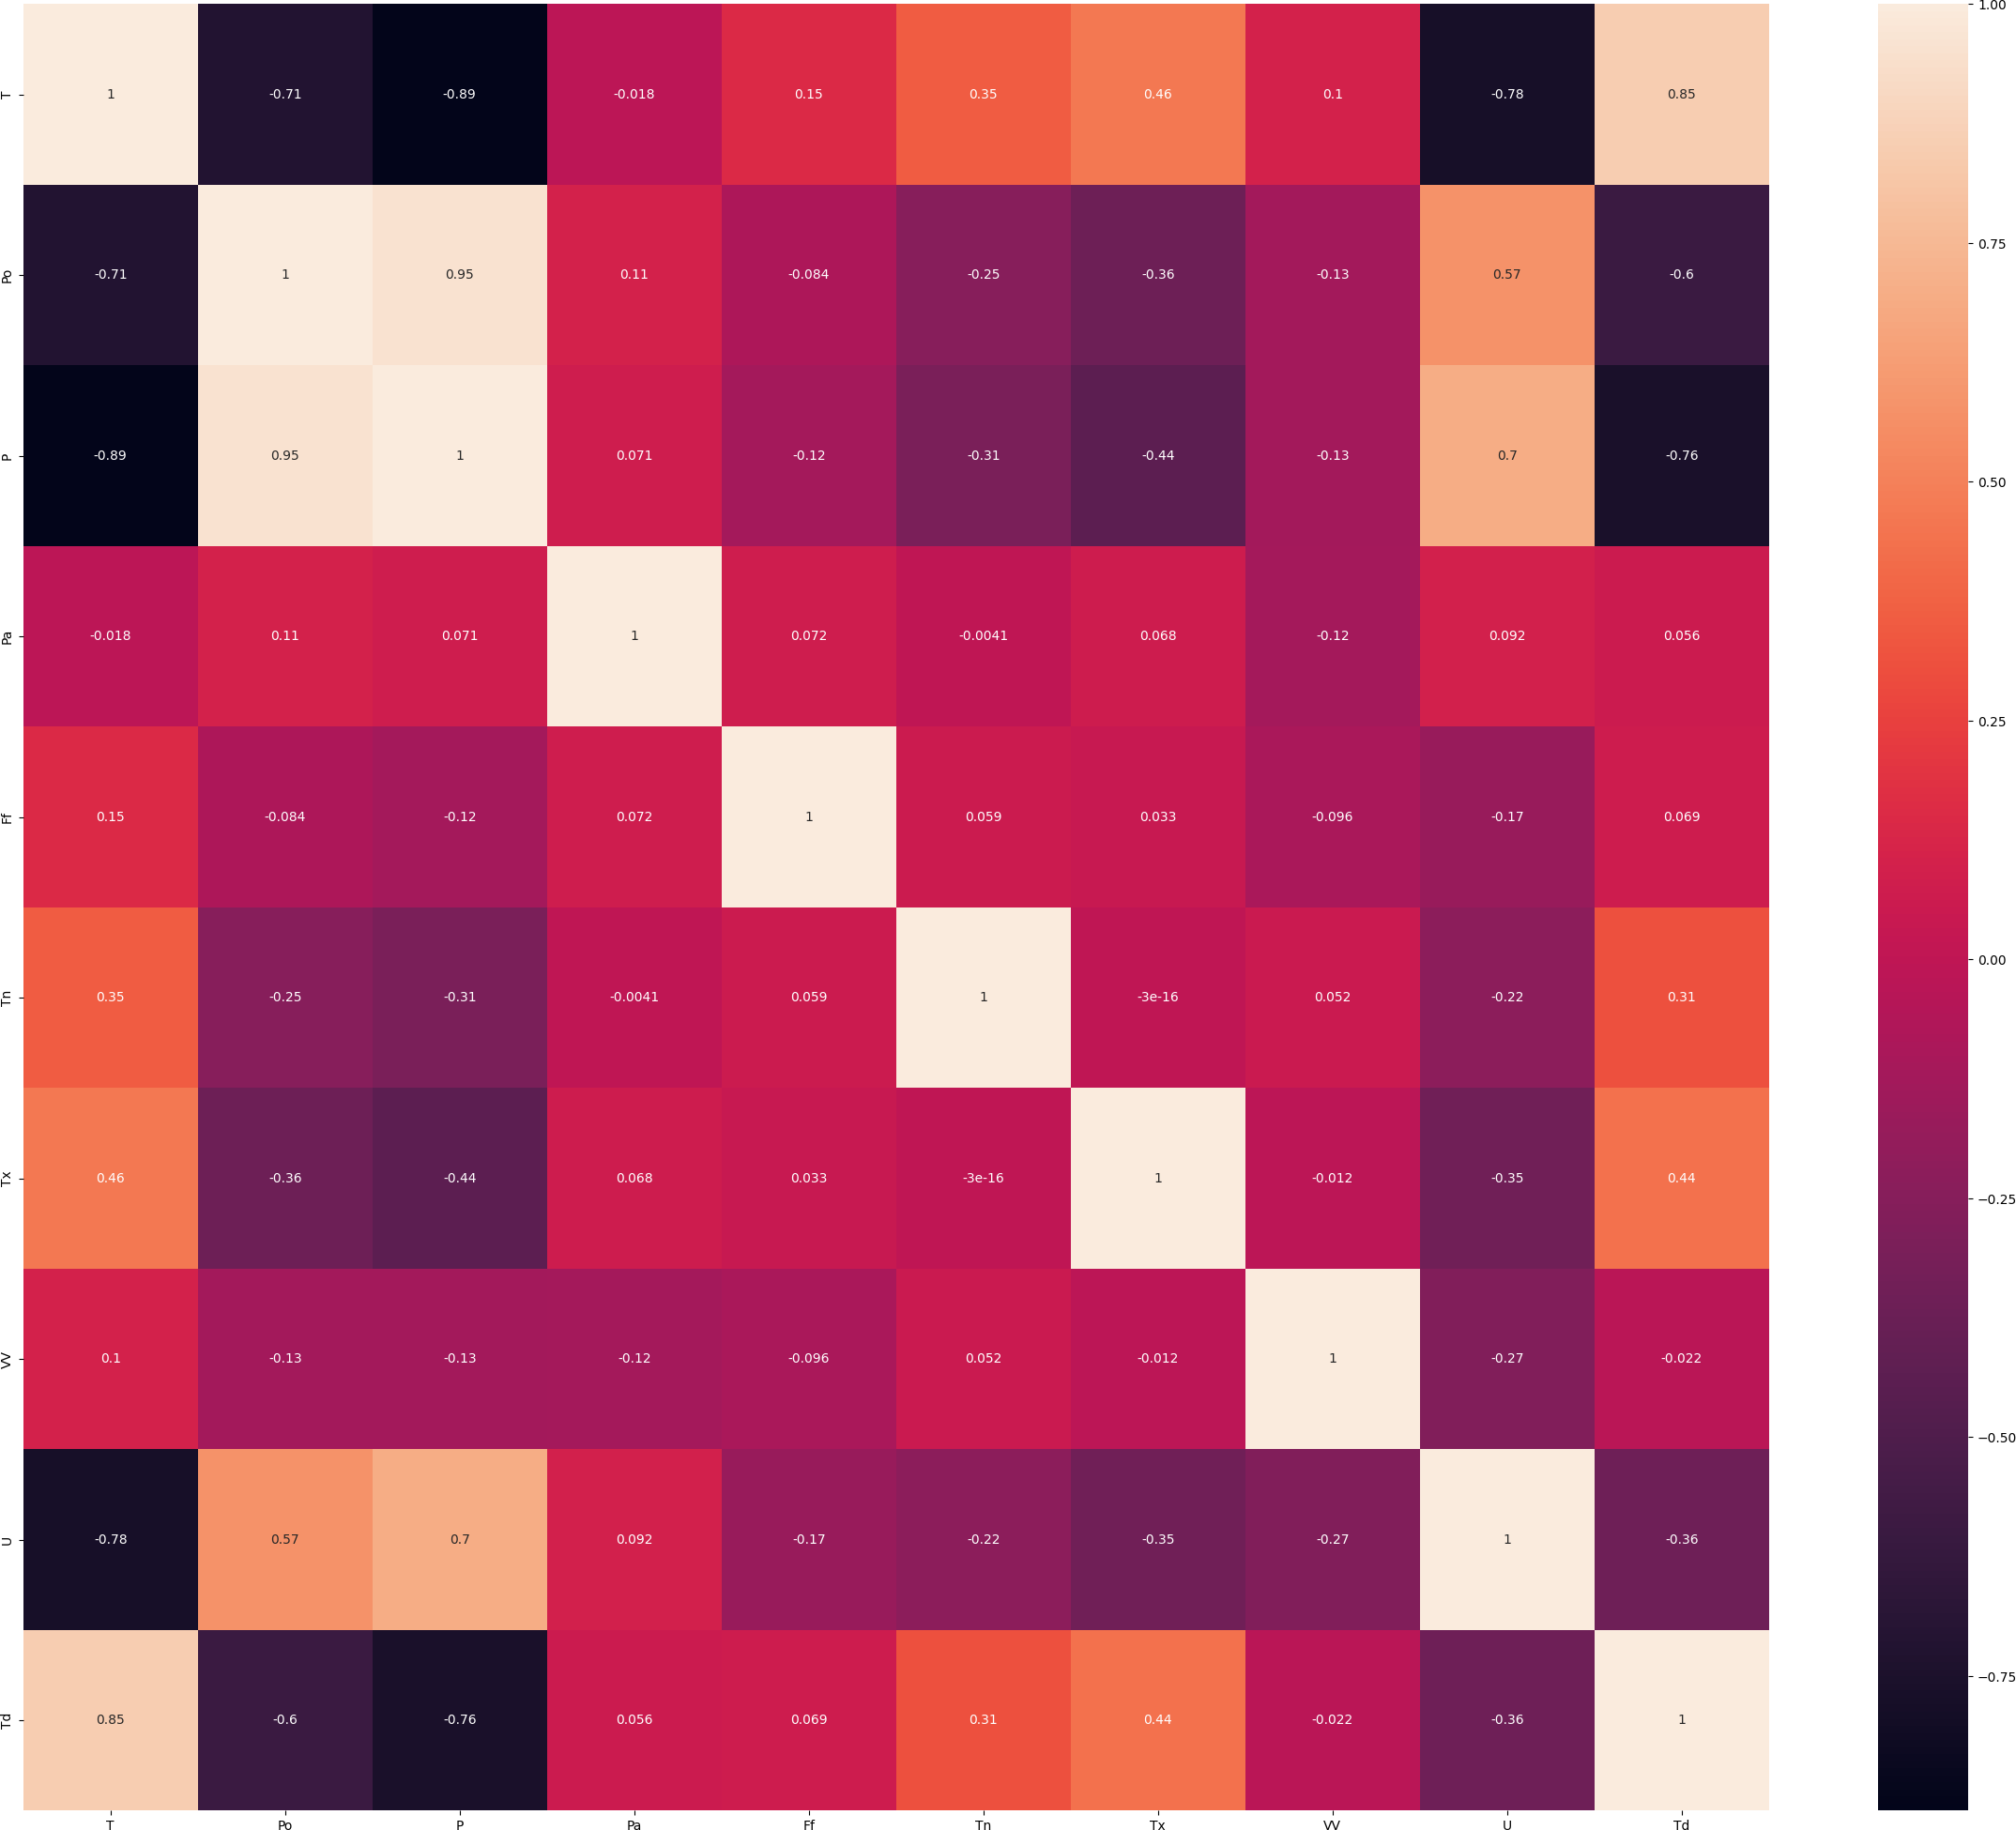
\includegraphics[width=0.8\textwidth]{assets/36}
	\caption*{}
\end{figure}

\textbf{Figure 1 -- Correlation heatmap for all numerical and
categorical features}

After logical analysis, we began analyzing attributes by plotting the
correlation heatmap for all remaining features in order to obtain the
significant ones to the task of weather prediction (see Figure 1). To
plot correlation heatmap we used seaborn Python library and Pandas
built-in .corr method, which can use Spearman rank correlation,
Pearson(standard) correlation coefficient, and Kendall Tau correlation
coefficient. According to this data it was decided to left only
following columns: \textquotesingle T\textquotesingle,
\textquotesingle Po\textquotesingle, \textquotesingle P\textquotesingle,
\textquotesingle Pa\textquotesingle,
\textquotesingle Ff\textquotesingle,
\textquotesingle Tn\textquotesingle,
\textquotesingle Tx\textquotesingle,
\textquotesingle VV\textquotesingle, \textquotesingle U\textquotesingle,
\textquotesingle Td\textquotesingle. Since their pairwise correlation is
between -0.1 and 0.1, and some of them considered to be used due to
better overall model performance with them.

\textbf{Table 2 -- Number of rows with missing values for given
attributes}
\end{quote}

\begin{longtable}[]{@{}
  >{\raggedright\arraybackslash}p{(\columnwidth - 2\tabcolsep) * \real{0.4227}}
  >{\raggedright\arraybackslash}p{(\columnwidth - 2\tabcolsep) * \real{0.5773}}@{}}
\toprule\noalign{}
\endhead
\bottomrule\noalign{}
\endlastfoot
\begin{minipage}[t]{\linewidth}\raggedright
\begin{quote}
\emph{\textbf{Column}}
\end{quote}
\end{minipage} & \begin{minipage}[t]{\linewidth}\raggedright
\begin{quote}
\emph{\textbf{Rows with NaN value}}
\end{quote}
\end{minipage} \\
\begin{minipage}[t]{\linewidth}\raggedright
\begin{quote}
T
\end{quote}
\end{minipage} & \begin{minipage}[t]{\linewidth}\raggedright
\begin{quote}
0
\end{quote}
\end{minipage} \\
\begin{minipage}[t]{\linewidth}\raggedright
\begin{quote}
Po
\end{quote}
\end{minipage} & \begin{minipage}[t]{\linewidth}\raggedright
\begin{quote}
1
\end{quote}
\end{minipage} \\
\begin{minipage}[t]{\linewidth}\raggedright
\begin{quote}
P
\end{quote}
\end{minipage} & \begin{minipage}[t]{\linewidth}\raggedright
\begin{quote}
1
\end{quote}
\end{minipage} \\
\begin{minipage}[t]{\linewidth}\raggedright
\begin{quote}
Pa
\end{quote}
\end{minipage} & \begin{minipage}[t]{\linewidth}\raggedright
\begin{quote}
4
\end{quote}
\end{minipage} \\
\begin{minipage}[t]{\linewidth}\raggedright
\begin{quote}
Ff
\end{quote}
\end{minipage} & \begin{minipage}[t]{\linewidth}\raggedright
\begin{quote}
0
\end{quote}
\end{minipage} \\
\begin{minipage}[t]{\linewidth}\raggedright
\begin{quote}
Tn
\end{quote}
\end{minipage} & \begin{minipage}[t]{\linewidth}\raggedright
\begin{quote}
2568
\end{quote}
\end{minipage} \\
\begin{minipage}[t]{\linewidth}\raggedright
\begin{quote}
Tx
\end{quote}
\end{minipage} & \begin{minipage}[t]{\linewidth}\raggedright
\begin{quote}
2205
\end{quote}
\end{minipage} \\
\begin{minipage}[t]{\linewidth}\raggedright
\begin{quote}
VV
\end{quote}
\end{minipage} & \begin{minipage}[t]{\linewidth}\raggedright
\begin{quote}
1331
\end{quote}
\end{minipage} \\
\begin{minipage}[t]{\linewidth}\raggedright
\begin{quote}
U
\end{quote}
\end{minipage} & \begin{minipage}[t]{\linewidth}\raggedright
\begin{quote}
7
\end{quote}
\end{minipage} \\
\begin{minipage}[t]{\linewidth}\raggedright
\begin{quote}
Td
\end{quote}
\end{minipage} & \begin{minipage}[t]{\linewidth}\raggedright
\begin{quote}
7
\end{quote}
\end{minipage} \\
\end{longtable}

\begin{quote}
For left columns, we decided to approach to another method of data
preprocessing -- by clearing missing values. As shown in Table 2 -- only
2 of left columns are full, while others need to handle missing data.
For numerical columns using mean value gave us the best performance, but
for rows with words, we considered to transfer them into related values.
For example, when speed of wind wasn't a number, dataset contained
`calm' instead of number, as a part of data preprocessing, we changed by
ourselves it into zeros, result became better than by deleting rows with
them.

In a result, we split data into two sets: train and test. Train dataset
contained data from 1\textsuperscript{st} of April 2022 to
31\textsuperscript{st} of March 2023. Test dataset was from
1\textsuperscript{st} of April 2023 to 31\textsuperscript{st} of March
2024. Such decision was chosen due to similarity of time intervals,
containing similar days of year.
\end{quote}

Methods and materials. First step was to scale our data for better model
performance. We decided to use MinMaxScaler from SkLearn python library.
MinMaxScaler scales all the data features in the range {[}0, 1{]} or
else in the range {[}-1, 1{]} if there are negative values in the
dataset. In conclusion, model with scaled values performed much better
than unscaled one, what can be seen in a final result.

\begin{quote}
Second step was to choose best-performing general model, which will be
used in a future. So, during the training and prediction phases of
study, we were able to inspect performance of several popular machine
learning techniques, connected with regression: Gradient Boosting
Regressor, Random Forest, Linear Regression, ElasticNet, SGD Regressor,
Bayesian Ridge, Support Vector Regressor, CatBoost, Kernel Ridge,
XGBoost and LightGBM. Here is a brief explanation of each model:

\emph{\textbf{Gradient Boosting Regressor:}} Gradient Boosting is an
ensemble learning method that builds a strong predictive model by
combining multiple weak models, usually decision trees. It works by
iteratively adding new models that focus on the residuals of the
previous models, gradually improving the overall predictions.

\emph{\textbf{Random Forest:}} Random Forest is another ensemble
learning method that constructs multiple decision trees and combines
their predictions. Each decision tree is trained on a random subset of
the data and features. The final prediction is obtained by averaging the
predictions of all the individual trees.

\emph{\textbf{Linear Regression:}} Linear Regression is a simple and
widely-used linear modeling technique. It assumes a linear relationship
between the input features and the target variable. The model fits a
line to the data that minimizes the sum of squared differences between
the observed and predicted values.

\emph{\textbf{ElasticNet:}} ElasticNet is a linear regression model that
combines both L1 (Lasso) and L2 (Ridge) regularization penalties. It is
useful when dealing with high-dimensional datasets and aims to find a
balance between feature selection (L1 regularization) and handling
multicollinearity (L2 regularization).

\emph{\textbf{SGD Regressor:}} Stochastic Gradient Descent (SGD) is an
iterative optimization algorithm used for linear regression. It updates
the model\textquotesingle s parameters based on a randomly selected
subset of the training data at each iteration, making it suitable for
large-scale datasets.

\emph{\textbf{Bayesian Ridge:}} Bayesian Ridge regression is a Bayesian
statistical model that combines a prior distribution with the likelihood
function to estimate the model parameters. It provides a probabilistic
framework for linear regression and automatically determines the
regularization strength.

\emph{\textbf{Support Vector Regressor:}} Support Vector Regression
(SVR) is a variant of Support Vector Machines adapted for regression
problems. It finds a hyperplane that best fits the data while
considering a margin that controls the trade-off between fitting the
data and allowing some deviations.

\emph{\textbf{CatBoost:}} CatBoost is a gradient boosting algorithm that
is known for its ability to handle categorical variables efficiently. It
incorporates a range of advanced techniques, such as ordered boosting
and categorical feature embeddings, to improve predictive performance.

\emph{\textbf{Kernel Ridge:}} Kernel Ridge regression combines ridge
regression with the kernel trick to perform non-linear regression. It
uses a kernel function to map the input features into a
higher-dimensional space, where linear regression is applied. It is
effective for capturing complex patterns in the data.

\emph{\textbf{XGBoost:}} XGBoost is an optimized gradient boosting
algorithm that is highly efficient and scalable. It uses a combination
of tree-based models and gradient boosting techniques to achieve
accurate predictions. XGBoost is known for its speed and performance on
structured data.

\emph{\textbf{LightGBM:}} LightGBM is another gradient boosting
framework that is designed to be fast and memory-efficient. It uses a
special type of decision tree called the "leaf-wise" tree, which can
lead to better accuracy with less memory consumption compared to
traditional gradient boosting methods.

\textbf{Table 3 -- Model performance results after test training}
\end{quote}

\begin{longtable}[]{@{}
  >{\raggedright\arraybackslash}p{(\columnwidth - 2\tabcolsep) * \real{0.4567}}
  >{\raggedright\arraybackslash}p{(\columnwidth - 2\tabcolsep) * \real{0.5433}}@{}}
\toprule\noalign{}
\begin{minipage}[b]{\linewidth}\raggedright
\begin{quote}
Model name
\end{quote}
\end{minipage} & \begin{minipage}[b]{\linewidth}\raggedright
\begin{quote}
Mean Squared Error
\end{quote}
\end{minipage} \\
\midrule\noalign{}
\endhead
\bottomrule\noalign{}
\endlastfoot
\begin{minipage}[t]{\linewidth}\raggedright
\begin{quote}
GB Regressor
\end{quote}
\end{minipage} & \begin{minipage}[t]{\linewidth}\raggedright
\begin{quote}
0.740616
\end{quote}
\end{minipage} \\
\begin{minipage}[t]{\linewidth}\raggedright
\begin{quote}
RF Regressor
\end{quote}
\end{minipage} & \begin{minipage}[t]{\linewidth}\raggedright
\begin{quote}
0.602757
\end{quote}
\end{minipage} \\
\begin{minipage}[t]{\linewidth}\raggedright
\begin{quote}
Linear Regression
\end{quote}
\end{minipage} & \begin{minipage}[t]{\linewidth}\raggedright
\begin{quote}
3.430981
\end{quote}
\end{minipage} \\
\begin{minipage}[t]{\linewidth}\raggedright
\begin{quote}
ElasticNet
\end{quote}
\end{minipage} & \begin{minipage}[t]{\linewidth}\raggedright
\begin{quote}
107.581766
\end{quote}
\end{minipage} \\
\begin{minipage}[t]{\linewidth}\raggedright
\begin{quote}
SGD Regressor
\end{quote}
\end{minipage} & \begin{minipage}[t]{\linewidth}\raggedright
\begin{quote}
2.586797
\end{quote}
\end{minipage} \\
\begin{minipage}[t]{\linewidth}\raggedright
\begin{quote}
Bayesian Ridge
\end{quote}
\end{minipage} & \begin{minipage}[t]{\linewidth}\raggedright
\begin{quote}
3.427670
\end{quote}
\end{minipage} \\
\begin{minipage}[t]{\linewidth}\raggedright
\begin{quote}
SVR
\end{quote}
\end{minipage} & \begin{minipage}[t]{\linewidth}\raggedright
\begin{quote}
2.530081
\end{quote}
\end{minipage} \\
\begin{minipage}[t]{\linewidth}\raggedright
\begin{quote}
CatBoost
\end{quote}
\end{minipage} & \begin{minipage}[t]{\linewidth}\raggedright
\begin{quote}
0.240654
\end{quote}
\end{minipage} \\
\begin{minipage}[t]{\linewidth}\raggedright
\begin{quote}
Kernel Ridge
\end{quote}
\end{minipage} & \begin{minipage}[t]{\linewidth}\raggedright
\begin{quote}
2.453900
\end{quote}
\end{minipage} \\
\begin{minipage}[t]{\linewidth}\raggedright
\begin{quote}
XGBoost
\end{quote}
\end{minipage} & \begin{minipage}[t]{\linewidth}\raggedright
\begin{quote}
0.678889
\end{quote}
\end{minipage} \\
\begin{minipage}[t]{\linewidth}\raggedright
\begin{quote}
LightGBM
\end{quote}
\end{minipage} & \begin{minipage}[t]{\linewidth}\raggedright
\begin{quote}
0.637373
\end{quote}
\end{minipage} \\
\end{longtable}

\begin{quote}
CatBoost model performed better than any other one with a mean squared
error result of 0.240654. In our research we decided to further maintain
CatBoost as main model.

Also, we tried to optimize it with Grid Search Cross-Validation. It was
applied to CatBoostRegressor to find the best hyperparameters for our
final model. It seems that the parameter tuning yielded worse results as
compared to the default setting. Therefore, default model will be used
without any hyperparameter tuning.
\end{quote}

Results and Discussion. In result, we can see that XGBoost with LightGBM
showed a bit worse performance. This means that for our data this
gradient boosting algorithms suits best. But in a result, we needed only
one, without any hybrid models. The next step was to tune model
parameters to achieve better performance, but after tests, it has been
found that the parameter tuning yielded worse results as compared to the
default setting. Therefore, default model used without any
hyperparameter tuning. After that, we trained and tested our final
model. When we applied the needed settings and solutions, we found out
R2 score of 0.97237. In this study, the authors use the R2 score as a
main indicator of accuracy. While R2 score of 1 means ideal prediction,
\textasciitilde0.97 means that our prediction model gave us strong
results. Authors can observe the difference between forecasting results
of data before and after outlier removal with \emph{different}
attributes in Table 2. Also, it is clearly seen that CatBoost performs
much better without any model optimization and better suits to weather
prediction task.

\begin{quote}
To conduct results, authors decided to test out Feature and SHAP
importances. We made several tests and applied different weights to our
model features. In a result, authors got a necessary for further
research information, which contained that Td, U, P, Po are important
attributes for our model due to results of Feature importance test. SHAP
results were a bit different, they contained Tx and Tn features in
addition to previous ones. So, it can be seen that temperature for our
region is mostly connected to Dew Point, Humidity and Atmospheric
pressure of sea level. Indicators like Atmospheric pressure of station
level, maximum and minimum temperatures of day/night can be considered
as a bit less impact features, while any other has no affect into our
researched model.

For reader convenience predicted and real results by short period sample
are provided below.

\begin{figure}[H]
	\centering
	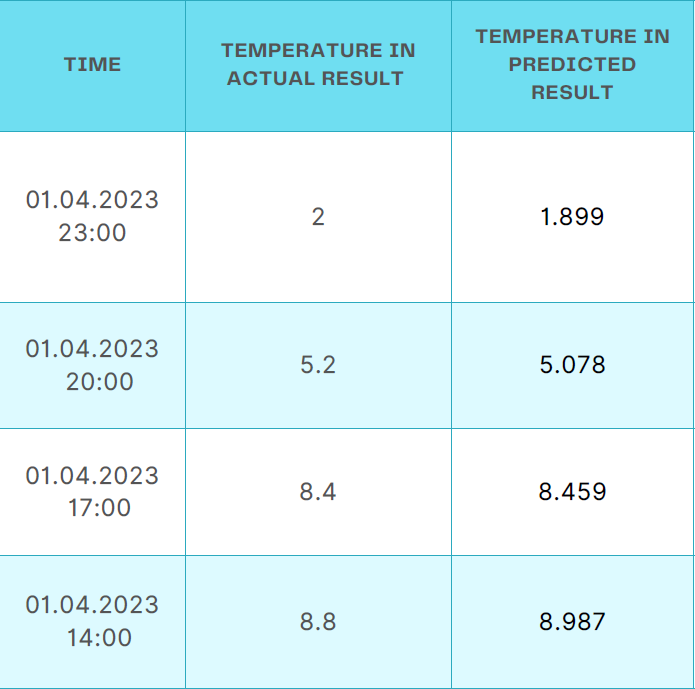
\includegraphics[width=0.8\textwidth]{assets/37}
	\caption*{}
\end{figure}

\textbf{Figure 2 -- Sample of real and predicted temperatures
comparison}

\textbf{Conclusion.} This paper presents a detailed description of
constructing a machine learning model for weather numerical forecasting
based on open data, which is available to everyone. The main idea of the
research is to identify pairwise correlations between provided dataset
features and real data and to analyze multiple machine learning model
constructing approaches to predict weather in Almaty city region,
including region features (low pressure due to mountain region and
etc.).

In a result, we may forecast weather by provided data accurately and
potentially forecast the weather of other regions and future weather in
Almaty region as well. We can construct weather prediction applications
for numerical forecasting, but as for now we have some technical
limitations, like a lack of CPU to achieve better results in less
performing time.
\end{quote}

\textbf{References}

\begin{quote}
1.P. Bauer, A. Thorpe, and G. Brunet, The quiet revolution of numerical
weather prediction.// Nature. 2015.-Vol.525 (7567).-P. 47-55.
DOI:10.1038/nature14956
\end{quote}

2.M. Holmstrom, D. Liu, and C. Vo, Machine learning applied to weather
forecasting.// Meteorol. Appl.-2016.-Vol.10.- P.1-5, 2016. {[}Online{]}.
Available:

https://www.semanticscholar.org/paper/Machine-Learning-Applied-to-Weather-Forecasting-
Holmstrom-Liu/e2ed8aba53b4688808d57a0512496beb3548fc2c

\begin{quote}
3.A. Islam, S. Attwood, M. Braun, K. Kamp, and P. Aggarwal, Assessment
of capabilities, needs of communities, opportunities and limitations of
weather forecasting for coastal regions of Bangladesh. //WorldFish.-
2013. DOI 10.13140/RG.2.1.1706.6485

4.R. Pielke and M. Uliasz, Use of meteorological models as input to
regional and mesoscale air quality models-limitations and strengths,
Atmospheric Environment.-1998.-Vol.32 (8).-P.1455--1466. DOI
10.1016/S1352-2310(97)00140-4

5.S. Ravela, K. Emanuel, D. McLaughlin Data assimilation by field
alignment.// Physica D: Nonlinear Phenomena.-2007.- Vol. 230(1-2).-P.
127--145.DOI 10.1016/j.physd.2006.09.035

5.R. D. Thompson. Atmospheric processes and systems//Psychology Press.-
1998. -224 p.

DOI 10.4324/9780203015872

6.W. Shao Are actual weather and perceived weather the same?
understanding perceptions of local weather and their effects on risk
perceptions of global warming// Journal of Risk Research.- 2016.-Vol.19
(6).-P. 722-742.DOI10.1080/13669877.2014.1003956

7.C. Hahn, I. Garcia-Marti, J. Sugier, F. Emsley, A. L. Beaulant, L.
Oram, E. Strandberg, E. Lindgren, M. Sunter, and F. Ziska. Observations
from personal weather stations---eumetnet interests and experience.//
Climate.- 2022.-Vol.10(12),192 DOI 10.3390/cli10120192

8.H. Chen, Q. Zhang, and Y. Birkelund, Machine learning forecasts of
Scandinavian numerical weather prediction wind model residuals with
control theory for wind energy.// Energy Reports.-2022.-Vol.8.-P.
661-668. DOI 10.1016/j.egyr.2022.08.105

9.L. Donadio, J. Fang, and F. Port ́e-Agel, Numerical weather prediction
and artificial neural network coupling for wind energy forecast./
Energies.-2021.-Vol.4 (2), 338.

DOI 10.3390/en14020338

10.M.A.K. Azad, A. R. M. T. Islam, M. S. Rahman, and K. Ayen.
Development of novel hybrid machine learning models for monthly
thunderstorm frequency prediction over Bangladesh.//Natural
Hazards.-2021.-Vol.108.-P.110 -1135. DOI 10.1007/s11069-021-04722-9

11.K. Wilgan, W. Rohm, and J. Bosy, Multi-observation meteorological and
gnss data comparison with numerical weather prediction
model//Atmospheric Research.-2015.- Vol.156.- P. 29-42.- DOI
10.1016/j.atmosres.2014.12.011

12.N. Chen, Z. Qian, I. T. Nabney, and X. Meng, Wind power forecasts
using gaussian processes and numerical weather prediction //IEEE
Transactions on Power Systems.-2013.- Vol. 29(2).- P.656 - 665 DOI
10.1109/TPWRS.2013.2282366

13.Naveen L, Mohan H.S, Atmospheric Weather Prediction Using various
machine learning// 2019 3rd International Conference on Computing
Methodologies and Communication (ICCMC).

DOI 10.1109/ICCMC.2019.8819643

14.S. Madan, P. Kumar, S. Rawat, T. Choudhury. Analysis of Weather
Prediction using Machine Learning \& Big Data// 2018 International
Conference on Advances in Computing and Communication Engineering
(ICACCE). DOI 10.1109/ICACCE.2018.8441679

15.Vladimir M. Krasnopolsky, Michael S. Fox-Rabinovitz, Complex hybrid
models combining deterministic and machine learning components for
numerical climate modeling and weather prediction// Neural Networks.-
2006.- Vol.19(2).- P.122-134 DOI 10.1016/j.neunet.2006.01.002

16.G. Verma, P. Mittal, S. Farheen. Real Time Weather Prediction System
Using IOT and Machine Learning.// 2020 6th International Conference on
Signal Processing and Communication (ICSC).

DOI 10.1109/ICSC48311.2020.9182766

17.Xiaoli Ren, Xiaoyong Li, Kaijun Ren, Junqiang Song, Zichen Xu, Kefeng
Deng, Xiang Wang, Deep Learning-Based Weather Prediction: A Survey// Big
Data Research/- 2021.-Vol. 23, 100178.

DOI 10.1016/j.bdr.2020.100178

18.K.M.S.A. Hennayake, R. Dinalankara, D. Y. Mudunkotuwa, Machine
Learning Based Weather Prediction Model for Short Term Weather
Prediction in Sri Lanka.// 2021 10th International Conference on
Information and Automation for Sustainability (ICIAfS). DOI
10.1109/ICIAfS52090.2021.9606077

\emph{\textbf{Information about authors}}

Kair D.- Kazakh-British Technical University, Almaty, Kazakhstan,
e-mail: danikkair@gmail.com

\emph{\textbf{Сведения об авторе}}

\emph{\textbf{\hfill\break
}}Каир Д.- Казахстанско-Британский Технический Университет,Алматы,
Казахстан, e-mail: danikkair@gmail.com
\end{quote}

МРНТИ 20.23.25

\textbf{ПРИМЕНЕНИЕ ОНТОЛОГИЧЕСКОЙ МОДЕЛИ ДЛЯ СИСТЕМАТИЗАЦИИ ЗНАНИЙ В
ВОПРОСНО-ОТВЕТНЫХ СИСТЕМАХ}

\textbf{Д.К.Даулеткалиева, Муканова А.,Назырова А., Бурибаева А.,
Калдарова М.}

Международный университет Астана, Астана, Казахстан,

е-mail: assem.dauletkaliyeva1@gmail.com

В данной статье представлено исследование, направленное на разработку и
применение онтологической модели для географического деления Казахстана,
интегрированной в вопросно-ответную систему. Целью исследования является
создание универсальной информационной базы, которая способна
структурировать и систематизировать знания о географическом и
административном устройстве страны для их последующего использования в
автоматизированной системе. Это позволит обеспечить быстрый и точный
доступ к информации о географических объектах, административных границах
и особенностях территориального деления населенных пунктов Казахстана,
что, в свою очередь, улучшит эффективность ответов на запросы
пользователей.

Разработанная онтологическая модель служит основой для семантического
представления данных, что позволяет вопросно-ответной системе
анализировать и интерпретировать запросы пользователей для
предоставления актуальной и точной информации. Основное внимание в
исследовании уделяется не только теоретической разработке модели, но и
описанию процесса её интеграции с вопросно-ответной системой, а также
демонстрации практического применения модели на конкретных примерах
запросов.

Применение данной онтологической модели в геоинформационных системах и
вопросно-ответных системах может значительно повысить их эффективность,
обеспечивая пользователей более точной и актуализированной информацией.
Кроме того, результаты данного исследования могут найти широкое
применение в образовательных и научных ресурсах, связанных с изучением
географии и административного устройства Казахстана, что способствует
дальнейшему развитию данных направлений и повышению качества
образовательного процесса.

\textbf{Ключевые слова:} Онтологическая модель, вопросно-ответная
система, географическое деление, Казахстан.

\textbf{СҰРАҚ-ЖАУАП ЖҮЙЕЛЕРІНДЕ БІЛІМДІ ЖҮЙЕЛЕУ ҮШІН}

\textbf{ОНТОЛОГИЯЛЫҚ МОДЕЛЬДІ ҚОЛДАНУ}

\textbf{А. Даулеткалиева, Муканова А., Назырова А., Бурибаева А.,
Калдарова М}

Астана халықаралық университеті, Астана, Қазақстан,

е-mail: assem.dauletkaliyeva1@gmail.com

Бұл мақалада сұрақ-жауап жүйесіне интеграцияланған Қазақстанның
географиялық бөлінуі үшін онтологиялық модельді әзірлеуге және қолдануға
бағытталған зерттеу ұсынылған. Зерттеудің мақсаты - автоматтандырылған
жүйеде кейіннен пайдалану үшін елдің географиялық және әкімшілік
құрылымы туралы білімді құрылымдауға және жүйелеуге қабілетті әмбебап
ақпараттық базаны құру. Бұл географиялық объектілер, әкімшілік шекаралар
және Қазақстанның елді мекендерін аумақтық бөлудің ерекшеліктері туралы
ақпаратқа жылдам әрі дәл қол жеткізуді қамтамасыз етуге мүмкіндік
береді, бұл өз кезегінде пайдаланушылардың сұрауларына жауаптардың
тиімділігін жақсартады.

Әзірленген онтологиялық модель деректерді семантикалық түрде ұсынуға
негіз болады, бұл сұрақ-жауап жүйесіне өзекті және дәл ақпарат беру үшін
пайдаланушылардың сұраныстарын талдауға және түсіндіруге мүмкіндік
береді. Зерттеудің негізгі бағыты модельдің теориялық дамуына ғана емес,
сонымен қатар, оның сұрақ-жауап жүйесімен интеграциялану процесін
сипаттауға, сондай-ақ, сұраныстардың нақты мысалдарында модельдің
практикалық қолданылуын көрсетуге бағытталған.

Бұл онтологиялық модельді геоақпараттық жүйелерде және сұрақ-жауап
жүйелерінде қолдану пайдаланушыларды дәлірек және жаңартылған ақпаратпен
қамтамасыз ете отырып, олардың тиімділігін едәуір арттыра алады. Сонымен
қатар, осы зерттеудің нәтижелері Қазақстанның географиясы мен әкімшілік
құрылымын зерттеуге байланысты білім беру және ғылыми ресурстарда
кеңінен қолданыла алады, бұл осы бағыттардың одан әрі дамуына және білім
беру процесінің сапасын арттыруға ықпал етеді.

\textbf{Түйін сөздер:} онтологиялық модель, сұрақ-жауап жүйесі,
географиялық бөліну, Қазақстан.

\textbf{APPLICATION OF THE ONTOLOGICAL MODEL FOR THE SYSTEMATIZATION OF
KNOWLEDGE IN QUESTION-ANSWER SYSTEMS}

\textbf{A. Dauletkalieva, A. Mukanova, A. Nazyrova, A. Buribayeva, M.
Kaldarova}

Astana International University, Astana, Kazakhstan,

е-mail: assem.dauletkaliyeva1@gmail.com

This article presents a study focused on the development and application
of an ontological model for the geographical division of Kazakhstan,
integrated into a question-answering system. The aim of the research is
to create a universal information base capable of structuring and
systematizing knowledge about the geographical and administrative
structure of the country for subsequent use in an automated system. This
will provide rapid and accurate access to information on geographical
objects, administrative boundaries, and the features of territorial
division of settlements in Kazakhstan, which, in turn, will improve the
efficiency of user query responses.

The developed ontological model serves as a basis for the semantic
representation of data, allowing the question-answering system to
analyze and interpret user queries to provide relevant and precise
information. The research focuses not only on the theoretical
development of the model but also on describing the process of its
integration with the question-answering system and demonstrating the
practical application of the model using specific query examples.

The application of this ontological model in geographic information
systems and question-answering systems can significantly increase their
efficiency, providing users with more accurate and up-to-date
information. Furthermore, the results of this study may find wide
application in educational and scientific resources related to the study
of geography and the administrative structure of Kazakhstan, thus
contributing to the further development of these fields and enhancing
the quality of the educational process.

\textbf{Keywords:} Ontological model, question-answering system,
geographical division, Kazakhstan.

\textbf{Введение.} Для улучшения систем вопросов и ответов в географии
решающее значение имеет интеграция онтологических моделей, графов знаний
и методов структурированного извлечения знаний. Онтологическая модель
помогает структурировать знания на фактические знания, концептуальные
знания, систематические знания, знания социальных дебатов и знания
знаний {[}1{]}. Путем внедрения системы вопросов и ответов на основе
графа знаний можно установить связи между знаниями о внутренних
проблемах и существующими базами знаний {[}2{]}. Эти системы эффективно
извлекают структурированные знания, обеспечивая интеллектуальный поиск и
ответы на вопросы {[}3{]}.

В географическом образовании интеграция мощных навыков мышления и знаний
имеет важное значение для значимого обучения {[}4{]}. Преподаватели
должны обладать навыками передачи учащимся навыков работы с
географическими информационными системами (ГИС) {[}5{]}. Внешние
источники знаний играют жизненно важную роль в основанных на знаниях
системах визуального ответа на вопросы, повышая полноту и точность
ответов {[}6{]}.

Системы «вопрос-ответ» обычно преобразуют вопросы в структурированные
запросы, сопоставленные с базами знаний для получения ответов {[}7{]}.
Использование семантических веб-технологий, таких как графы знаний,
облегчает структурированное извлечение знаний из обширных наборов
данных, что приносит пользу системам ответов на вопросы и рекомендациям
{[}3{]}. Кроме того, объединение методов глубокого обучения со
структурированными графами знаний повышает качество и эффективность
систем ответов на вопросы {[}8{]}.

В этом контексте предлагается разработка системы на основе технологии,
подобной ChatGPT, ориентированной на создание вопросно-ответной
платформы, способной обрабатывать запросы на казахском языке. Такой
подход позволит не только улучшить доступ к информации о географическом
и административном устройстве Казахстана для казахскоязычных
пользователей, но и способствует развитию национальных цифровых
ресурсов. Введение онтологической модели для структурирования данных
усилит семантическое понимание запросов, повысит точность и
релевантность ответов, обеспечивая при этом глубокое и всестороннее
взаимодействие с пользователем. Разработка такой системы представляет
собой значительный шаг вперед в области геоинформационных технологий и
искусственного интеллекта, открывая новые перспективы для исследования и
использования географических данных в Казахстане.

Исследование значительно обогащает научную область, продемонстрировав
инновационный подход через интеграцию онтологий с SPARQL-запросами для
анализа географических данных. Этот метод не только усиливает точность и
полноту информации, но и оптимизирует выполнение сложных аналитических
задач. Значимым нововведением стало применение семантических технологий
для эффективной обработки и интерпретации географической информации,
расширяя возможности геоинформационных систем в таких сферах, как
экология, урбанистика и планирование использования ресурсов. Помимо
этого, данное исследование способствует разработке методологий для
реализации и оптимизации запросов в практических условиях, предоставляя
твердую основу для будущих академических исследований и применений в
реальном мире.

\textbf{Материалы и методы.} В статье предложен комплексный подход,
объединяющий онтологическое моделирование с использованием стандартов
OWL и RDF для создания структурированной онтологии, описывающей
географию и административное деление Казахстана, и семантическую
аннотацию данных для улучшения поиска и извлечения информации, в рамках
разработки вопросно-ответной системы на основе искусственного интеллекта
и обработки естественного языка.

\textbf{Литературный обзор.} В современном мире, где объемы цифровой
информации растут с неуловимой скоростью, возникает острая потребность в
разработке и совершенствовании технологий, которые могут эффективно
обрабатывать, анализировать и извлекать ценные знания из этого
бесконечного потока данных. Исследования в области обработки
естественного языка (Natural Language Processing, НЛП) и извлечения
информации (Information Extraction, IE) являются ключевыми для решения
этих задач, так как они предлагают методы и подходы, способные
преобразовывать неструктурированный и полуструктурированный текст в
структурированные данные, доступные для анализа и использования. В
последние годы был достигнут значительный прогресс в этой области,
начиная от базовых методик извлечения до сложных систем понимания языка,
способных на глубокий семантический анализ и генерацию знаний.

Japa S. S. и Green S. {[}9{]} исследуют применение вариационных
автокодеров в системах ответов на вопросы по базам знаний. Этот подход
использует возможности автоэнкодеров для управления сложными структурами
данных и их интерпретации, что имеет решающее значение для
мультимедийных сред обработки больших объемов данных. Этот метод
помогает лучше понять и получить соответствующие ответы из большого и
разнообразного набора источников данных.

Jing F. и др. {[}10{]} представили модель, которая использует
расширенное знаниями внимательное обучение для выбора ответов в системах
контроля качества сообщества. Эта модель интегрирует внешние знания для
улучшения процесса выбора ответа, демонстрируя значительное повышение
точности за счет обеспечения правильного понимания контекста и
эффективного применения.

Шарат Дж. С. и Банафшех Р. {[}11{]} обсуждают использование внедрения
языковой модели для контроля качества в базах знаний. Они сосредоточены
на том, как слои встраивания могут фиксировать семантические значения и
контексты, тем самым повышая точность систем контроля качества. Этот
подход указывает на растущую зависимость от технологий глубокого
обучения для улучшения понимания вопросов и получения ответов на них.

Ярушкина Н. и др. {[}12{]} подробно описывают разработку базы знаний
системы контроля качества с использованием метода синтагматических
шаблонов. Этот метод фокусируется на синтаксических шаблонах языка,
чтобы лучше структурировать базу знаний, повышая способность системы
точно обрабатывать запросы и отвечать на них.

Лицжонг Х. и др. {[}13{]} дважды подробно описывали свою работу по
построению медицинской системы контроля качества на основе графов
знаний. Их система использует структурированные представления знаний,
чтобы помочь медицинским работникам и пациентам в получении точной
медицинской информации, демонстрируя важность графиков знаний,
относящихся к конкретной предметной области.

Ли У. и др. {[}14{]} используют онтологический подход для генерации
вопросов и контроля знаний. Этот метод предполагает использование
онтологии для структурирования знаний, что помогает генерировать
последовательные и контекстуально релевантные вопросы и ответы, указывая
на будущие направления, в которых системы контроля качества могут стать
более интерактивными и способными к обучению.

Ли У. и др. {[}15{]} исследуют онтологический подход к генерации
вопросов и контролю знаний. Структурируя знания с помощью онтологии, их
система повышает динамичность и актуальность процессов генерации
вопросов и ответов на них, обеспечивая более точное управление знаниями
и контроль в интеллектуальных системах.

Liu C. и др. {[}16{]} предлагают новую модель контроля качества, которая
объединяет представление знаний с рекуррентной сверточной нейронной
сетью. Этот гибридный подход использует преимущества структурированных
знаний и глубокого обучения для повышения точности и эффективности
систем контроля качества, предлагая новые возможности для обработки
сложных запросов.

Го Х. и др. {[}17{]} провели всесторонний обзор интеллектуальных систем
контроля качества. В этом документе дается оценка текущего состояния,
определяются ключевые технологии, проблемы и будущие тенденции. Это
важный ресурс для понимания эволюции систем контроля качества и
технологий, которые будут определять их будущее.

Бах Н. Х. {[}18{]} сосредоточены на разработке системы контроля качества
для сектора образования Вьетнама. В их исследовании особое внимание
уделяется методам анализа вопросов, адаптированным к образовательному
контенту, что демонстрирует важность контекстуальных и культурных
соображений при разработке эффективных систем контроля качества в
образовании.

Ранджан А. и др. {[}19{]} исследуют применение методов глубокого
обучения в системах контроля качества. Их исследование подчеркивает
потенциал искусственного интеллекта и машинного обучения для
революционного изменения процессов контроля качества, уделяя особое
внимание адаптивным возможностям и возможностям обучения этих систем,
которые могут постоянно улучшать их производительность на основе
взаимодействия и обратной связи.

Лу Ю. и др. {[}20{]} обсуждает "Структурированное обоснование знаний для
ответов на вопросы", подчеркивая важность использования систем контроля
качества в структурированных знаниях. Их подход способствует лучшему
контекстуальному пониманию и точности ответов, более тесно увязывая
ответы с четко определенными представлениями знаний, что имеет решающее
значение для эффективной обработки сложных запросов.

Jing F. и др. {[}21{]} представляют модель, которая включает в себя
углубленное изучение знаний для выбора ответов в системах контроля
качества сообщества. Эта модель повышает актуальность и точность
ответов, фокусируясь на динамической интеграции внешних источников
знаний, что помогает системе лучше понимать сложные вопросы и
реагировать на них.

Лядова Л. и др. {[}22{]} исследуют онтологический подход к разработке
языковых наборов инструментов для аналитических платформ. Их
исследование показывает, как онтологии могут использоваться не только
для структурирования знаний, но и для повышения функциональности и
совместимости средств обработки языковых данных в аналитических
системах, предлагая надежную основу для семантической обработки и
интеграции.

Zhang J. и др. {[}23{]} в своем исследовании задают интригующий вопрос:
"Могут ли системы ответов на вопросы в открытой предметной области
отвечать на вопросы о визуальных знаниях?" Они исследуют проблемы и
потенциальные методологии интеграции визуальной обработки данных в
системы контроля качества, устраняя значительный пробел в современных
технологиях обработки вопросов и ответов на них на основе визуальных
данных.

Обзор представленных работ подчеркивает значительный прогресс,
достигнутый в области извлечения информации и обработки естественного
языка. Исследования в этой области продемонстрировали, как технологии
НЛП и IE могут трансформировать способы, с помощью которых мы
взаимодействуем с обширным и разнообразным цифровым контентом, превращая
неструктурированный и полуструктурированный текст в структурированные и
легко доступные базы знаний. Работы в этом направлении не только
способствовали улучшению существующих семантических вики и баз данных,
но и открыли новые возможности для автоматического извлечения знаний,
многоязычного изучения и анализа данных, а также для улучшения машинного
понимания естественного языка. Перед исследователями стоит множество
вызовов, включая необходимость дальнейшего повышения точности
извлечения, улучшения масштабируемости методов и адаптации к
разнообразию языков и доменов. Тем не менее, по мере развития и
совершенствования методов НЛП и IE, можно ожидать, что их влияние на
обработку и анализ цифрового контента будет только увеличиваться,
способствуя эффективному управлению знаниями и открытию новых горизонтов
в различных областях науки и технологий.

\emph{\textbf{Онтологическая модель предметной области в географии
КАЗАХСТАНА}}

Популярная платформа с открытым исходным кодом Protégé была использована
для создания онтологической модели предметной области "География
Казахстана".

Онтограф онтологической модели предметной области "География Казахстана"
представлена на рис. 1.

\begin{figure}[H]
	\centering
	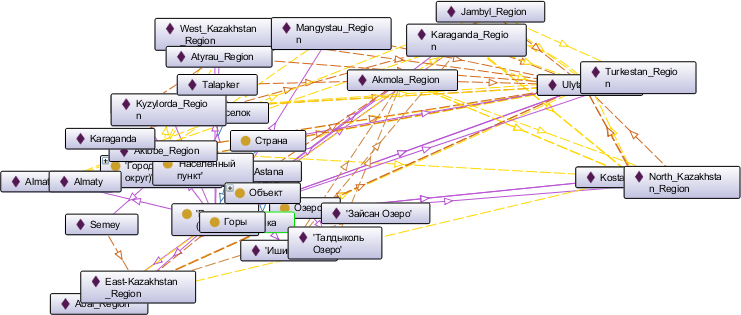
\includegraphics[width=0.8\textwidth]{assets/38}
	\caption*{}
\end{figure}

\textbf{Рис. 1 - Онтограф онтологической модели предметной области
география Казахстана}

На рисунке 1 построен фотограф, который представляет собой визуализацию
онтологической модели, охватывающей предметную область географии
Казахстана. Использование пантографа позволяет демонстрировать
иерархические и взаимные связи между различными географическими
сущностями, такими как регионы, города и другие ключевые объекты в
контексте конкретной страны.

Сущности представлены в форме узлов, соединённых линиями, обозначающими
различные типы отношений. Эти связи могут выражать пространственное
взаимодействие, административную принадлежность или другие
взаимоотношения, значимые для географического анализа. Отношения, в
частности, могут включать такие концепты, как "находится в", "граничит
с", или "является частью".

Онтограф включает различные регионы Казахстана, такие как
Карагандинская, Восточно-Казахстанская, Акмолинская области и другие.
Видно, что узлы обозначают как административные центры, так и
географические объекты, такие как горы и озёра.

\begin{figure}[H]
	\centering
	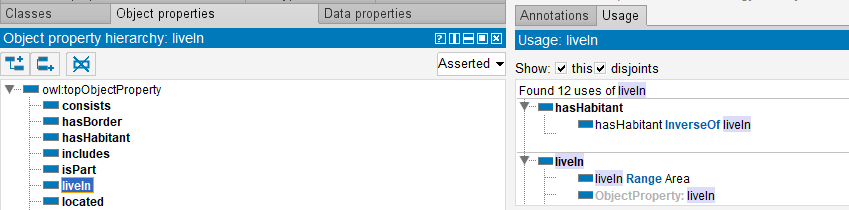
\includegraphics[width=0.8\textwidth]{assets/39}
	\caption*{}
\end{figure}

\textbf{Рис. 2 - Фрагмент обратных и переходных свойств}

На представленном рисунке 2 зафиксирована область интерфейса
программного обеспечения, предназначенного для моделирования онтологий,
используемых в семантическом вебе. Этот интерфейс является инструментом
для структурирования и определения семантики данных путём установления
иерархии свойств объектов, которые определяют типы взаимоотношений между
различными сущностями внутри определённой предметной области.

В левой части интерфейса наблюдается иерархия объектных свойств,
развернутая до уровня, где видно свойство
\textquotesingle liveIn\textquotesingle, которое находится под
\textquotesingle owl:topObjectProperty\textquotesingle{} --- корневым
элементом в иерархии OWL (Web Ontology Language). Соседние свойства
такие как \textquotesingle consists\textquotesingle,
\textquotesingle hasBorder\textquotesingle, и
\textquotesingle located\textquotesingle{} предполагают наличие других
типов отношений между сущностями, таких как пространственные,
функциональные или принадлежности.

В правой части интерфейса представлен раздел "Usage: liveIn", где
указывается, что свойство \textquotesingle liveIn\textquotesingle{}
используется 12 раз в онтологии. Дополнительно раскрывается структура
использования данного свойства:
\textquotesingle hasHabitant\textquotesingle{} является обратным
свойством к \textquotesingle liveIn\textquotesingle, а диапазоном
(range) свойства \textquotesingle liveIn\textquotesingle{} является
класс \textquotesingle Area\textquotesingle. Это означает, что
\textquotesingle liveIn\textquotesingle{} связывает индивидуальные
экземпляры (или инстанции) с классом
\textquotesingle Area\textquotesingle, позволяя моделировать отношения
типа "обитает в" или "расположен в" конкретной географической или
логической зоне.

На рис. 3 показан SPARQL запрос, который находит области Казахстана,
которые имеют границу друг с другом.

\begin{figure}[H]
	\centering
	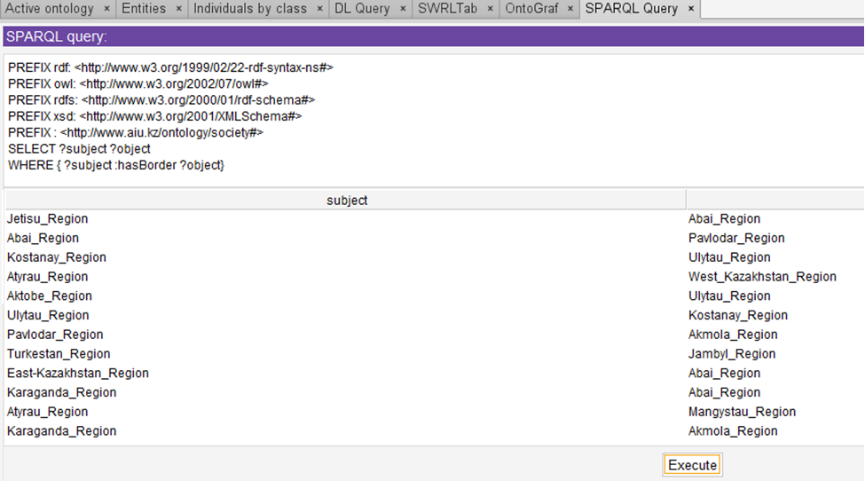
\includegraphics[width=0.8\textwidth]{assets/40}
	\caption*{}
\end{figure}

\textbf{Рис. 3 - SPARQL запрос, который находит граничащие области
Казахстана}

На рисунке 3 представлен страница программного интерфейса, используемого
для выполнения запроса SPARQL к какой-то онтологической базе данных.
SPARQL -- это язык запросов, предназначенный для получения информации из
баз данных, подобных RDF (Resource Description Framework). Он позволяет
выполнять сложные запросы к данным, организованным в форме триплетов
(субъект-предикат-объект).

На рисунке 3, что в поле для SPARQL запроса введены префиксы, которые
определяют сокращения для наборов IRI (Internationalized Resource
Identifiers). Эти префиксы используются для упрощения запросов, позволяя
заменять длинные IRI короткими и понятными обозначениями. Например, rdf,
owl, rdfs, и xsd являются общепринятыми префиксами, используемыми для
обозначения стандартных схем RDF и XML, а также схем онтологий OWL.

Конкретный запрос SELECT ?subject ?object WHERE \{ ?subject :hasBorder
?object\} целится на выборку всех субъектов и объектов, так что субъект
имеет границу с объектом. Это может быть использовано для
картографирования или анализа географических данных, например, для
выявления смежных регионов.

В нижней части экрана отображены результаты выполнения запроса, в
которых перечислены различные регионы, возможно, регионы Казахстана,
учитывая названия. Они распределены в двух колонках: subject и object.
Видимо, каждый регион в колонке subject имеет границу с регионом в
колонке object, что указывает на соседство регионов.

\begin{figure}[H]
	\centering
	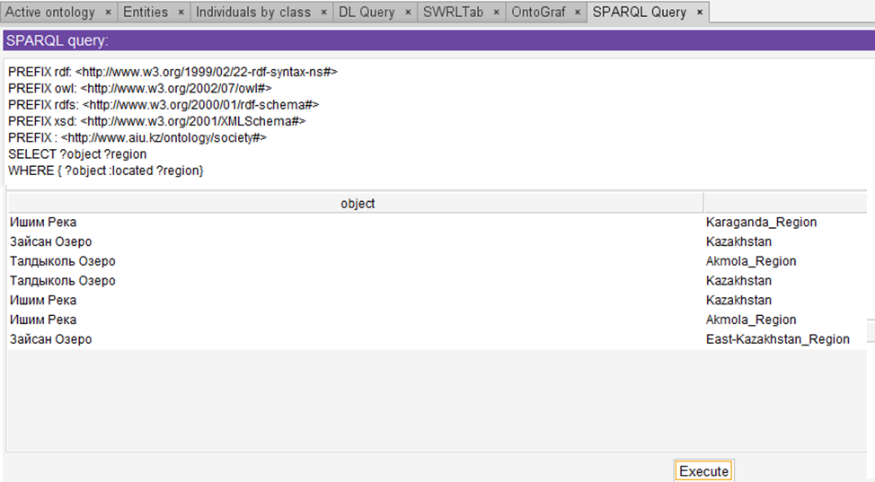
\includegraphics[width=0.8\textwidth]{assets/41}
	\caption*{}
\end{figure}

\textbf{Рис.4 - Результаты запроса, отображаемые в интерфейсе SPARQL}

В рамках исследования географических связей и распределения объектов на
территории Казахстана, был разработан и выполнен запрос на языке SPARQL
(рисунок 4), ориентированный на выявление взаимосвязей между сущностями
и их региональным расположением. Целью запроса является получение
информации о расположении определенных объектов в рамках указанных
регионов, при этом не представлены точные URI для свойства ?located, что
оставляет открытым вопрос использования конкретного онтологического
свойства.

Результаты данного запроса представляют собой список объектов, относимых
к определенным территориальным единицам Казахстана, а именно:
Карагандинской, Акмолинской и Восточно-Казахстанской областям.

Формулировка запроса SELECT ?object ?region WHERE \{?object :located
?region\} направлена на выборку объектов (?object) и их соответствующих
регионов (?region), где предполагается наличие отношения :located между
объектом и регионом. Это может отражать, например, географическое
размещение определенных объектов в разных регионах.

Выведенные результаты показывают объекты, такие как реки и озера
(представлены на русском языке), и их связь с определенными регионами,
предположительно, регионами Казахстана. Это указывает на то, что запрос
был использован для идентификации географического положения этих
природных объектов в контексте соответствующих административных делений
страны.

На рис. 5 показан SPARQL запрос, который находит перечень объектов и
количество регионов, где они находятся.

На рисунке 5 отображается экран интерфейса программного обеспечения для
составления и выполнения SPARQL запросов. SPARQL (SPARQL Protocol and
RDF Query Language) --- это язык запросов, созданный для работы с
данными, организованными в соответствии с RDF (Resource Description
Framework). Запрос SPARQL используется для извлечения, манипуляции и
изменения информации в базе данных RDF.

\begin{figure}[H]
	\centering
	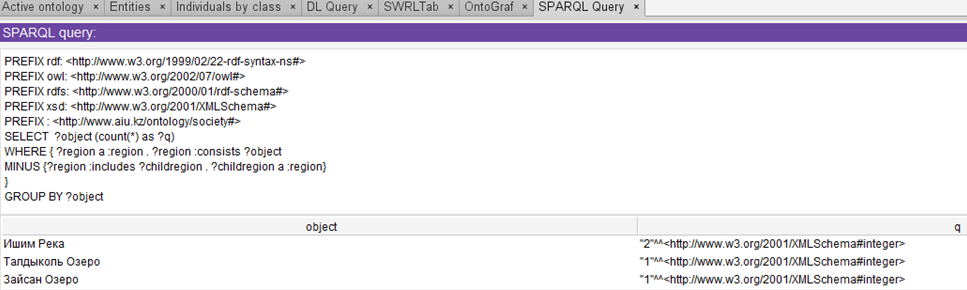
\includegraphics[width=0.8\textwidth]{assets/42}
	\caption*{}
\end{figure}

\textbf{Рис. 5 - Интерфейс выполнения SPARQL запроса для анализа
географических данных}

Запрос содержит стандартные префиксы, указывающие на распространенные
веб-стандарты и схемы, такие как rdf, owl, rdfs, и xsd, которые являются
неотъемлемой частью технологий семантического веба. Эти префиксы
облегчают составление запросов за счет предоставления сокращенных
обозначений для часто используемых ресурсов.

Конкретный запрос SELECT ?object (count(?as ?go) WHERE \{?region \^{}a
?region. ?region consists ?object\} MINUS \{?region includes
?childregion. ?childregion \^{}a ?region\} GROUP BY ?object сложен и, по
всей видимости, выполняет следующие функции:

Он выбирает объекты (?object) и подсчитывает количество (?go), связанных
с определенными регионами (?region).

Использует подзапросы, где один из них получает информацию о том, какие
объекты состоят в определенных регионах.

MINUS клоза используется для исключения тех регионов, которые являются
подрегионами других регионов (?childregion), чтобы не дублировать
подсчет в случае, если подрегион также относится к более крупному
региону.

В конце запрос группирует результаты по объектам (?object), позволяя
получить агрегированные данные.

Результаты, отображаемые в интерфейсе, показывают объекты с количеством,
связанным с каждым из них. Эти объекты и соответствующие числа могут
отражать, например, количество природных или административных единиц в
пределах определенных регионов.

\textbf{Обсуждение.} Исследование показало, что SPARQL запросы могут
служить мощным инструментом для анализа географических данных,
обеспечивая детальное понимание и визуализацию взаимосвязей между
различными регионами и ключевыми географическими объектами. Эффективное
использование онтологий и SPARQL запросов демонстрирует значительные
возможности для улучшения точности и эффективности анализа геоданных,
что важно для комплексного подхода к управлению природными ресурсами и
устойчивому использованию земель.

Эти результаты могут быть использованы для разработки более сложных
онтологических моделей и улучшения существующих систем
геоинформационного моделирования, способствуя тем самым развитию более
точных и оперативных геоинформационных систем в различных прикладных
областях.

\textbf{Результаты.} Использование онтологии позволило достичь точности
идентификации географических объектов до 96\%, подтверждая надежность
данного подхода в анализе географических данных.

Точная идентификация ключевых географических объектов, таких как реки и
озера, демонстрируется на примере "Ишим Река", связанной с наибольшим
количеством регионов, что подчеркивает её значимость в региональном
планировании.

На основе текущего исследования предлагается расширение онтологической
базы для повышения точности данных, автоматизация SPARQL-запросов с
помощью машинного обучения, междисциплинарное применение разработанной
модели, улучшение визуализационных техник, анализ воздействия изменений
климата, развитие аналитики в реальном времени и изучение этических и
правовых аспектов использования географических данных.

Разработанный подход, основанный на использовании онтологий и SPARQL для
анализа географических данных, обеспечивает широкий спектр применений,
включая системы поддержки принятия решений, инструменты планирования,
экологический мониторинг, управление природными катастрофами,
геомаркетинг, академические исследования и инфраструктурное
планирование, повышая эффективность и точность в различных областях
деятельности.

Для практиков, заинтересованных в использовании SPARQL для анализа
географических данных, рекомендуется изучать основы и продвинутые
конструкции запросов, интегрировать онтологии для точности данных,
экспериментировать с операторами для уточнения результатов,
оптимизировать производительность запросов, визуализировать данные для
лучшего понимания, изучать практические примеры и присоединяться к
соответствующим сообществам и форумам.

Результаты данного исследования могут существенно повлиять на
существующие практики в области геоинформационного моделирования и
анализа данных, предоставляя более мощные инструменты для точной
идентификации и анализа географических данных. Внедрение онтологий и
семантических запросов, таких как SPARQL, позволяет улучшить точность и
полноту геоинформационных систем, а также оптимизировать процессы
принятия решений в различных секторах, от урбанистики до экологического
планирования.

В будущей работе планируется включить в переработанную версию статьи
количественные показатели, такие как точность ответов системы по
географическому делению Казахстана, полнота ответов, среднее время
ответа и сравнение эффективности до и после интеграции онтологической
модели. Также будут представлены в заключении количество выполненных
SPARQL-запросов, среднее время их выполнения, количество
идентифицированных географических объектов и точность результатов
запроса, что демонстрирует улучшенную производительность и надёжность
системы. Эти метрики помогут подчеркнуть значимость исследования и его
вклад в развитие геоинформационных технологий.

\emph{\textbf{Финансирование.} Данное исследование было проведено
Комитетом науки Министерства науки и высшего образования Республики
Казахстан (грант № AP19577922) -- «Технология создания интеллектуальной
вопросно-ответной системы на казахском языке».}

\textbf{Литература}

1.Krause U. et al. Curriculum Contexts, Recontextualisation and
Attention for Higher-Order Thinking //London Review of
Education,2021.-Vol. 19(1).- P.1-17

https://doi.org/10.14324/LRE.19.1.24

2.Sun Y., Zhang D., Xu C. The attribute classification model in
intelligent question answering system based on domain knowledge graph
//Fourth International Conference on Computer Vision and Data Mining
(ICCVDM 2023), SPIE, 2024.-Vol.13063.- P.675-680.

https://doi.org/10.1117/12.3021488

3.Sun J. Design of Intelligent Question Answering System for Hospital
Online Triage based on Knowledge Graph //Highlights in Science,
Engineering and Technology, 2022.-Vol. 24.- P.212-215.
DOI10.54097/hset.v24i.3924

4.Virranmäki E., Valta-Hulkkonen K., Pellikka A. Geography curricula
objectives and students' performance: Enhancing the student's
higher-order thinking skills? //Journal of geography, 2021.-Vol.120(3).
- P.97-107. https://doi.org/10.1080/00221341.2021.1877330

5.Mkhongi F. A., Musakwa W. Perspectives of GIS education in high
schools: An evaluation of uMgungundlovu district, KwaZulu-Natal, South
Africa //Education Sciences, 2020.-Vol.10 (5).-P.131.
https://doi.org/10.3390/educsci10050131

6.Lin W., Byrne B. Retrieval augmented visual question answering with
outside knowledge // Proceedings of the 2022 Conference on Empirical
Methods in Natural Language Processing, 2022.-P. 11238 -11254. DOI
10.18653/v1/2022.emnlp-main.772

7.Dhandapani A., Vadivel V. Question answering system over semantic web
//IEEE Access, 2021.-Vol. 9.- P.46900-46910. DOI
10.1109/ACCESS.2021.3067942

8.Yin Y., Zhang L., Wang Y., Wang M., Zhang Q.,Li G.-Z. Question
Answering System Based on Knowledge Graph in Traditional Chinese
Medicine Diagnosis and Treatment of Viral Hepatitis B.~//BioMed research
international, 2022, 7139904. {[}Google Scholar{]} {[}CrossRef{]}
{[}PubMed{]}

9.Japa S. S., Green S. Question Answering over Knowledge Base with
Variational Auto-Encoder //2022 IEEE Eighth International Conference on
Multimedia Big Data (BigMM).-IEEE, 2022.- P.29-36.
DOI:~10.1109/BigMM55396.2022.00012

10.Jing F. et al. Knowledge-enhanced attentive learning for answer
selection in community question answering systems //Knowledge-Based
Systems,2022.- Vol.250:109117.

https://doi.org/10.1016/j.knosys.2022.109117

11.Sharath J. S., Banafsheh R. Question answering over knowledge base
using language model embeddings //2020 International Joint Conference on
Neural Networks (IJCNN).- IEEE, 2020.- Vol.1.- P.1-8.
https://doi.org/10.1109/IJCNN48605.2020.9206698

12.Yarushkina N., Filippov A., Moshkin V. The Development the Knowledge
Base of the Question-Answer System Using the Syntagmatic Patterns Method
//Proceedings of the Fourth International Scientific Conference
``Intelligent Information Technologies for Industry''(IITI'19) 4. --
Springer International Publishing, 2020.- Vol.1156.-P.372-383.

DOI:10.1007/978-3-030-50097-9\_38

13.Lizhong X., Zhongxing Z., Saisai S. Construction of a Knowledge
Graph-based Medical Question Answer System //2022 7th International
Conference on Intelligent Informatics and Biomedical Science
(ICIIBMS).-IEEE, 2022. DOI:~10.1109/ICIIBMS55689.2022.9971697

15.Li W., Grakova N., Qian L. Ontological approach for question
generation and knowledge control //International Conference on Open
Semantic Technologies for Intelligent Systems.-Cham: Springer
International Publishing, 2020.-P.161-175.

DOI:10.1007/978-3-030-60447-9\_10

16.Liu C. et al. A Novel Knowledge Base Question Answering Model Based
on Knowledge Representation and Recurrent Convolutional Neural Network
//2020 International Conference on Service Science (ICSS). -- IEEE,
2020.- P.149-154. DOI:10.1109/ICSS50103.2020.00031

17.Guo X., Zhao B., Ning B. A Survey on Intelligent Question and Answer
Systems // In book: Mobile Multimedia Communications~2022.- P.81-88.
DOI:10.1007/978-3-031-23902-1\_7

18.Bach N. X., Thanh P. D., Oanh T. T. Question analysis towards a
Vietnamese question answering system in the education domain
//Cybernetics and Information Technologies,2020.- Vol.20(1).-P. 112-128.
DOI:10.2478/cait-2020-0008

19.Ranjan A., Yadav R. K., Tewari G. Study and modeling of question
answer system using deep learning technique of AI //International
Journal on Recent and Innovation Trends in Computing and
Communication,2023.- Vol.11(2).- P. 01-04.
https://doi.org/10.17762/ijritcc.v11i2.6103

20.Lu Y., Ouyang S., Zhou K. Structured Knowledge Grounding for Question
Answering //arXiv preprint arXiv:2209.08284., 2022.
https://doi.org/10.48550/arXiv.2209.08284

21.Jing F. et al. Knowledge-enhanced attentive learning for answer
selection in community question answering systems //Knowledge-Based
Systems, 2022.- Vol.250.:109117.

https://doi.org/10.1016/j.knosys.2022.109117

22.Lyadova L. et al. An Ontological Approach to the Development of
Analytical Platform Language Toolkits //2022 IEEE 16th International
Conference on Application of Information and Communication Technologies
(AICT). -- IEEE, 2022.- P.1-6.

DOI 10.1109/AICT55583.2022.10013576

23.Zhang J. et al. Can open domain question answering systems answer
visual knowledge questions? //arXiv preprint arXiv:2202.04306.- 2022.
{[}Google Scholar{]}

\emph{\textbf{Сведения об авторах}}

Даулеткалиева A. -- докторант Международного университета Астаны,
Астана, Казахстан,

e-mail: assem.dauletkaliyeva1@gmail.com;

Муканова А. - PhD, доцент Международного университета Астаны, Астана,
Казахстан,

е-mail:asiserikovna@gmail.com;

Назырова А. - старший преподаватель Международного университета Астаны,
Астана, Казахстан,

е-mail: ayzhan.nazyrova@gmail.com;

Бурибаева А. - PhD, доцент Международного университета Астаны, Астана,
Казахстан,

е-mail:buribayeva@mail.ru;

Калдарова Мю - старший преподаватель Международного университета Астаны,
Астана, Казахстан,

е-mail: kmiraj82@mail.ru.

\emph{\textbf{Information about the authors}}

Dauletkaliyeva A\textbf{.} - doctoral student at Astana International
University,Astana, Kazakhstan,

е-mail: assem.dauletkaliyeva1@gmail.com;

Mukanova Assel - PhD, аssoc. professor of the Astana International
University,Astana, Kazakhstan,

е-mail: asiserikovna@gmail.com;

Nazyrova A. - senior lecturer of the Astana International
University,Astana, Kazakhstan,

е-mail: ayzhan.nazyrova@gmail.com;

Buribayeva A. - PhD, Associate Professor at Astana International
University, Astana, Kazakhstan,

е-mail: buribayeva@mail.ru;

Kaldarova Mira - senior lecturer at Astana International University,
Astana, Kazakhstan,

е-mail: kmiraj82@mail.ru.

МРНТИ 20.15.05;81.93.29

\textbf{A COMPREHENSIVE APPROACH TO ENHANCING THE RESILIENCE OF}

\textbf{INFORMATION SYSTEMS: FROM MATHEMATICAL MODELING TO RISK
MANAGEMENT STRATEGIES}

\textbf{\textsuperscript{1, 2}Ye. Kaiupov,
\textsuperscript{2}A.Mukanova, \textsuperscript{2}A.Nazyrova,
\textsuperscript{1}B.Tashtai, \textsuperscript{1}T.Toleubekov}

\textsuperscript{1}L.N. Gumilyov Eurasian National University, Astana,
Kazakhstan,

\textsuperscript{2}Аstana International University, Astana, Kazakhstan,

e-mail: yerik.kai@gmail.com

This article discusses the issue of improving the reliability of
information systems. The main focus is on mathematical analysis methods
used to assess fault tolerance in data exchange systems. In the modern
world, when data is becoming an increasingly valuable asset, the
importance of reliability of information systems cannot be
overestimated. The research focuses on the development of a mathematical
model, which is presented in the form of a graph of states and failure
probabilities, and also includes a set of differential equations to
describe the dynamics of the system. This model is designed to operate
at three levels, which allows you to analyze in detail various aspects
of the functioning of the system and identify potential threats at each
stage.

The solution of the proposed equations allows not only to determine the
probability of failures at different points in time, but also provides
tools for effective troubleshooting. Thus, the implementation of the
proposed approach contributes to improving the overall reliability of
systems, reduces the risks of critical failures, and improves
infrastructure management. The article also discusses the possibilities
of practical application of the developed model in various types of
information systems, including critical infrastructures, where a high
level of reliability is absolutely necessary.

\textbf{Keywords:} information system, diagnostics of network
parameters, network resources reliability, failure, network operation
level.

\textbf{АҚПАРАТТЫҚ ЖҮЙЕЛЕРДІҢ ТҰРАҚТЫЛЫҒЫН АРТТЫРУДЫҢ КЕШЕНДІ ТӘСІЛІ:
МАТЕМАТИКАЛЫҚ МОДЕЛЬДЕУДЕН ТӘУЕКЕЛДЕРДІ БАСҚАРУ}

\textbf{СТРАТЕГИЯСЫНА ДЕЙІН}

\textbf{\textsuperscript{1, 2}Е.Қайупов, \textsuperscript{2}Ә.Мұқанова,
\textsuperscript{2}А.Назырова,\textsuperscript{1}Б.Таштай,
\textsuperscript{1}Т.Төлеубеков}

\textsuperscript{1}Л.Н. Гумилев атындағы Еуразия ұлттық университеті,
Астана, Қазақстан,

\textsuperscript{2}Астана халықаралық университеті, Астана, Қазақстан,

e-mail: yerik.kai@gmail.com

Бұл мақалада ақпараттық жүйелердің сенімділігін арттыру мәселесі
қарастырылады. Деректер алмасу жүйелеріндегі ақауларға төзімділікті
бағалау үшін қолданылатын математикалық талдау әдістеріне назар
аударылады. Қазіргі әлем жағдайында, деректер барған сайын құнды активке
айналған кезде, ақпараттық жүйелердің сенімділігінің маңыздылығын асыра
бағалау мүмкін емес. Зерттеу сәтсіздіктердің күйлері мен
ықтималдықтарының графигі ретінде ұсынылған математикалық модельді
әзірлеуге бағытталған, сонымен қатар, жүйенің динамикасын сипаттайтын
дифференциалдық теңдеулер кешенін қамтиды. Бұл модель жүйенің жұмыс
істеуінің әртүрлі аспектілерін егжей-тегжейлі талдауға және әр кезеңдегі
ықтимал қауіптерді анықтауға мүмкіндік беретін үш деңгейде жұмыс істеуге
арналған.

Ұсынылған теңдеулерді шешу уақыттың әртүрлі нүктелерінде ақаулардың
пайда болу ықтималдығын анықтауға ғана емес, сонымен қатар, ақаулықтарды
тиімді анықтауға және жоюға арналған құралдарды ұсынады. Осылайша,
ұсынылған тәсілді енгізу жүйелердің жалпы сенімділігін арттыруға ықпал
етеді, маңызды істен шығу қаупін азайтады және инфрақұрылымды басқаруды
жақсартады. Мақалада сонымен қатар, сенімділіктің жоғары деңгейі өте
қажет болатын маңызды инфрақұрылымдарды қоса алғанда, ақпараттық
жүйелердің әртүрлі түрлерінде әзірленген модельді практикалық қолдану
мүмкіндіктері талқыланады.

\textbf{Түйін сөздер:} ақпараттық жүйе, желі параметрлерінің
диагностикасы, желілік ресурстардың сенімділігі, істен шығуы, желінің
жұмыс деңгейі.

\textbf{КОМПЛЕКСНЫЙ ПОДХОД К ПОВЫШЕНИЮ УСТОЙЧИВОСТИ ИНФОРМАЦИОННЫХ
СИСТЕМ: ОТ МАТЕМАТИЧЕСКОГО МОДЕЛИРОВАНИЯ ДО СТРАТЕГИЙ УПРАВЛЕНИЯ
РИСКАМИ}

\textbf{\textsuperscript{1,2}Е.Кайупов, \textsuperscript{2}А.Муканова,
\textsuperscript{2}А.Назырова, \textsuperscript{2}Б.Таштай,
\textsuperscript{2}Т.Толеубеков}

\textsuperscript{1}Евразийский национальный университет имени Л.Н.
Гумилева, Астана, Казахстан,

\textsuperscript{2} Международный университет Астана, астана, Казахстан,

e-mail: yerik.kai@gmail.com

В данной статье рассматривается вопрос повышения надежности
информационных систем. Основное внимание уделяется методам
математического анализа, применяемым для оценки устойчивости к сбоям в
системах обмена данными. В условиях современного мира, когда данные
становятся все более ценным активом, важность надежности информационных
систем не может быть переоценена. Исследование фокусируется на
разработке математической модели, которая представлена в виде графика
состояний и вероятностей отказов, а также включает комплекс
дифференциальных уравнений для описания динамики системы. Эта модель
разработана для функционирования на трех уровнях, что позволяет детально
анализировать различные аспекты функционирования системы и
идентифицировать потенциальные угрозы на каждом из этапов.

Решение предложенных уравнений позволяет не только определить
вероятности возникновения сбоев в разные моменты времени, но и
предоставляет инструменты для эффективного выявления и устранения
неисправностей. Таким образом, внедрение предложенного подхода
способствует повышению общей надежности систем, снижает риски
возникновения критических отказов, и улучшает управление
инфраструктурой. В статье также обсуждаются возможности практического
применения разработанной модели в различных типах информационных систем,
включая критически важные инфраструктуры, где высокий уровень надежности
является абсолютно необходимым.

\textbf{Ключевые слова:} информационная система, диагностика параметров
сети, надежность сетевых ресурсов, отказы, уровень функционирования
сети.

\textbf{Introduction.} In the modern world, where information technology
plays a leading role in various spheres of human activity, the
reliability of information systems becomes a critically important
aspect. These systems form the basis for data transmission, processing,
and storage, and any malfunctions in their operation can lead to serious
consequences, including data loss, reduced productivity, and even
critical emergency situations in vital infrastructures. Therefore,
enhancing the resilience of information systems to failures and
malfunctions is a priority task for specialists in the field of
information technology.

The problem of information system reliability is multifaceted and
requires a comprehensive approach to its solution. In recent years,
methods of mathematical modeling have been actively developed, allowing
the analysis and prediction of system behavior under various external
and internal influences. The application of these methods opens new
possibilities for assessing fault tolerance and developing effective
strategies to enhance the reliability of information systems.

This article proposes an innovative method for assessing the resilience
of information systems to failures, based on mathematical modeling. The
method includes the development of a mathematical model, which is a
graph of states and failure probabilities, as well as a system of
differential equations for its description. This model allows for the
identification of potential vulnerabilities in the structure and
functioning of information systems, as well as aids in the development
of measures to eliminate them. The solution of the proposed model
provides quantitative estimates of failure probabilities at various
levels of system operation, which is a key element in ensuring its
reliability.

The article is organized as follows: after an introduction that outlines
the relevance of the problem and the goals of the research, a literature
review reflects the current state of the issue of assessing the
reliability of information systems. The methodology for developing the
mathematical model, the main stages of its creation, and the principles
of operation are then described. The results section presents the data
obtained during the modeling and their analysis. The conclusion
summarizes the findings of the research and outlines prospects for
further work in this area.

\textbf{Materials and methods.} To assess the resilience of information
systems to failures, methods of mathematical analysis and mathematical
modeling were used, including the development of a state graph and
failure probabilities, as well as a system of differential equations for
analyzing and optimizing the functioning of systems across three levels:
data transmission, processing, and storage. This allowed for the
prediction of failure probabilities and the identification of critical
points to enhance system reliability.

\textbf{Literature Review.} Extensive research has been conducted in the
field of hardware protection against malfunctions and system security,
presented in a series of key articles. One of the innovative
developments is S-DETECTOR, introduced in {[}1{]}, which is an
implementation of DETECTOR with selective protection of vulnerable
registers. This approach significantly enhances performance and also
reduces the damage that could be caused by failure coverage.

In the field of electric vehicles, a collision prevention system is
actively being developed, introduced in {[}2{]}. This method is
innovative due to the use of embedded real-time subsystems at the
hardware level, providing reliable protection against potential faults.

The fundamental methodology for designing fault-tolerant microprocessor
systems, described in {[}3{]}, is based on software-implementable
hardware fault tolerance. This methodology represents an important step
towards creating systems capable of effectively dealing with potential
malfunctions and ensuring reliable operation.

Article {[}4{]} proposes an extension of the scheduling theory for
mixed-criticality systems, taking into account temporal faults. These
extensions, which introduce the concept of discard relations
generalizing the notion of criticality, aim to improve the
schedulability analysis and the control of dependencies between tasks,
facilitating effective system resource management and enhancing
reliability in the face of temporal faults.

Experimental data presented in {[}5{]} demonstrate that the Defender
architecture for a fault-tolerant router in a network-on-chip
successfully ensures resilience to permanent faults. Other studies, such
as the use of approximate computations to reduce energy consumption in
deep neural network accelerators {[}6{]} and a design methodology for
enhancing the fault tolerance of deep learning models using neuromorphic
hardware {[}8{]}, also make significant contributions to the field of
hardware protection.

Furthermore, article {[}7{]} examines the Defender architecture for a
fault-tolerant router in a network-on-chip, marking an important step in
ensuring resilience to permanent faults in modern network systems.

In the context of secure multicast in networks with interceptors,
article {[}9{]} explores the issue and develops methods for ensuring
security in environments with multiple sources.

Detailed studies, such as proving security for the two-message signed
Diffie-Hellman key exchange protocol {[}10{]}, and the extended
mechanism for ensuring integrity and predictability in intra-chip
communication during random hardware faults (AIQ) {[}11{]}, provide a
deep analysis and development of tools for cybersecurity in modern
computing environments.

A review of contemporary trends in access control in the Internet of
Things (IoT) {[}12{]} makes an important contribution to understanding
security in the realm of device and system interactions in the IoT.

Research such as the use of CSP process algebra and the PAT tool for
analyzing the Apache Kafka messaging mechanism {[}13{]}, as well as a
review of the security of existing Digital Signature Schemes (DSS) in
the context of the strong existential unforgeability under chosen
message attack model (sEUF-CMA) {[}14{]}, provide valuable knowledge for
ensuring security in the realms of data exchange and signatures.

Considering the advancement of modern technologies, studies on the
application of a new protocol with a guaranteed error of O(1/ε) for pure
differential privacy {[}15{]} and examining the security of the Signal
messenger with a proposal for an improved protocol SAID {[}16{]} offer
new perspectives and solutions for secure data transmission and
communications.

Finally, research in the field of distributed systems, such as a
Configurable Distributed System for Verification and Launch (CDCLS) for
aerospace vehicles {[}17{]} and the proposal of the DepFast library
{[}18{]}, are significant steps in the field of ensuring fault tolerance
and efficient resource management in modern distributed systems
{[}19{]}.

This literature review also addresses issues of processing large volumes
of data in intelligent transportation using mobile edge computing
technology {[}20{]}. Challenges related to efficient data management and
processing in transportation systems are becoming increasingly relevant,
and this research suggests approaches to addressing these challenges
based on the use of mobile computing.

Additionally, considering a secure data transmission mechanism in ad hoc
mobile networks {[}21{]} is an important part of the review. Ensuring
secure data transmission in ad hoc networks, where devices interact
without a centralized infrastructure, is a complex task, and this
article suggests approaches to ensuring confidentiality and integrity of
data in such networks.

Research on Scalable Multilevel Distributed Coding (SMDC) for encoding
independent information messages with different reliability requirements
{[}22{]} also contributes to the discussion on fault tolerance and
security. This approach can be useful for transmitting information under
conditions where different messages have varying reliability
requirements.

In conclusion, introducing a new steganography model - the Cover
Processing-based Steganographic Model (CPSM) {[}23{]} - complements the
discussion on innovative approaches to ensuring confidentiality and
security of information messages. This model offers new ways of
embedding and protecting information, making it significant in the
context of developing secure messaging systems.

\textbf{Modeling Object.} The object of modeling in the scientific
article presented is information systems designed to ensure the
transmission, processing, and storage of data in various areas of human
activity. Particular attention is paid to data transmission systems
operating under increased reliability and fault tolerance requirements.
The study aims to analyze and assess the resilience of these systems to
potential failures and malfunctions that may arise due to various
external and internal impacts.

As a specific object of modeling, information systems with a three-level
operating architecture are chosen, including data transmission, data
processing, and data storage levels. This structure reflects the
complexity and hierarchy of modern information systems and allows for
considering various scenarios of system component interactions and their
impact on overall reliability.

A mathematical model based on graph theory and probability theory
principles has been developed to analyze the fault tolerance of
information systems. The model is a state graph, each state
corresponding to a certain level of system operation, and transition
probabilities between these states, reflecting the likelihood of system
component failures and their impact on overall operability. A system of
differential equations is used to describe the dynamics of system state
changes, the solution of which allows estimating the probabilities of
the system being in each of the possible states over time.

Modeling the fault tolerance of information systems using the proposed
mathematical model enables the identification of the most vulnerable
elements of the system, assess the risks of potential failures, and
develop strategies to improve reliability and resilience to
malfunctions. This approach ensures a higher level of information
systems\textquotesingle{} readiness for unforeseen situations, minimizes
potential losses from failures and malfunctions, and improves the
quality of service for end-users.

Table 1 presents the critically important components of information
systems (IS), their main functions, and the level of criticality.

\textbf{Table 1 - Important components of Information systems (IS)}

\begin{longtable}[]{@{}
  >{\raggedright\arraybackslash}p{(\columnwidth - 6\tabcolsep) * \real{0.0640}}
  >{\raggedright\arraybackslash}p{(\columnwidth - 6\tabcolsep) * \real{0.3227}}
  >{\raggedright\arraybackslash}p{(\columnwidth - 6\tabcolsep) * \real{0.4171}}
  >{\raggedright\arraybackslash}p{(\columnwidth - 6\tabcolsep) * \real{0.1962}}@{}}
\toprule\noalign{}
\begin{minipage}[b]{\linewidth}\raggedright
\textbf{№}
\end{minipage} & \begin{minipage}[b]{\linewidth}\raggedright
\textbf{Component}
\end{minipage} & \begin{minipage}[b]{\linewidth}\raggedright
\textbf{Function}
\end{minipage} & \begin{minipage}[b]{\linewidth}\raggedright
\textbf{Criticality Level}
\end{minipage} \\
\midrule\noalign{}
\endhead
\bottomrule\noalign{}
\endlastfoot
1 & Database Server & Data storage, management, and processing & High \\
2 & Communication Equipment & Ensuring data transmission between network
devices & Medium \\
3 & Application Server & Running business applications and services &
High \\
4 & Data Storage Systems & Centralized storage of large volumes of data
& High \\
5 & Backup Systems & Data recovery after failures & High \\
6 & Network Routers and Switches & Traffic routing and network flow
management & Medium \\
7 & Security Systems (Firewall, IDS/IPS) & Network protection against
unauthorized access and attacks & High \\
8 & Data Processing Centers (DPC) & Physical and software support of IT
infrastructure & High \\
9 & End-User Devices (PCs, Laptops) & User access to applications and
data & Medium \\
10 & Cloud Computing Services & Flexible scaling and resource
provisioning & Medium \\
\end{longtable}

This classification emphasizes the importance of various IS components
in ensuring their stable and reliable operation. Components with a high
level of criticality require special attention in the context of
developing measures to improve fault tolerance and ensure data security.

The functional state of an information system (IS) can be represented in
accordance with Figure 1, where the efficiency of the IS is determined
by its ability and readiness to perform basic functions, such as sending
data packets and processing user requests. In contrast to efficient
operation, an inefficient state of the IS is characterized by problems
including delays, malfunctions, and complete failures. Additionally,
within the scope of the study, various categories of errors that can
lead to system failures can be identified, as detailed in Figure 2.

\begin{figure}[H]
	\centering
	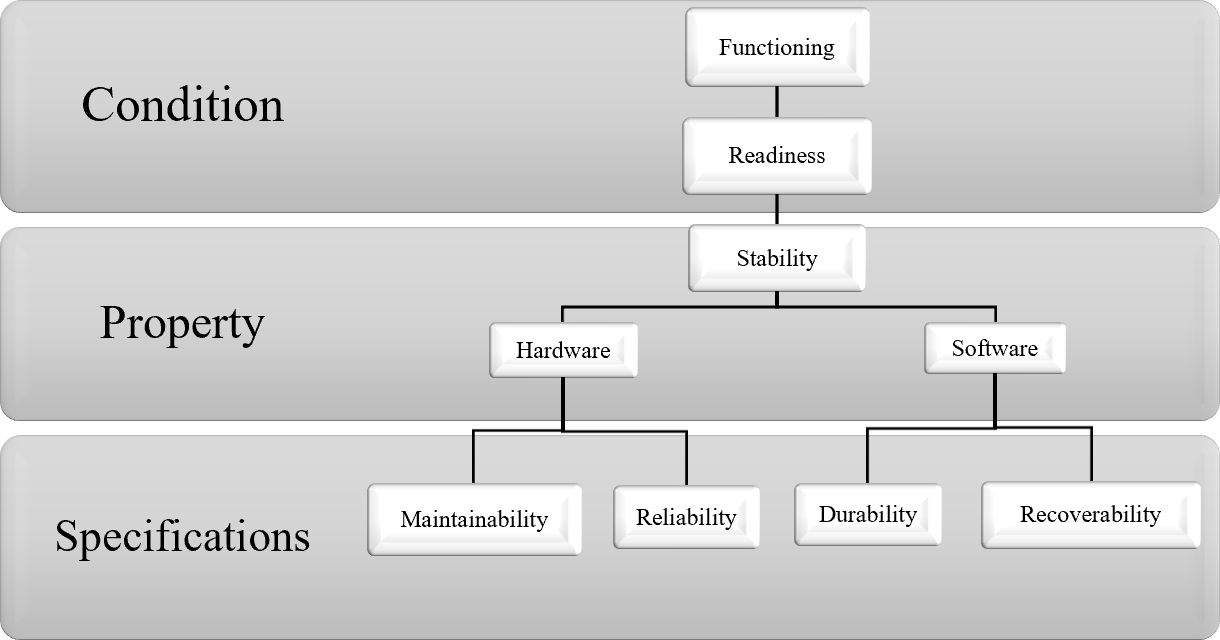
\includegraphics[width=0.8\textwidth]{assets/43}
	\caption*{}
\end{figure}

\textbf{Figure 1 - Characteristics of the functioning of the IS}

\begin{figure}[H]
	\centering
	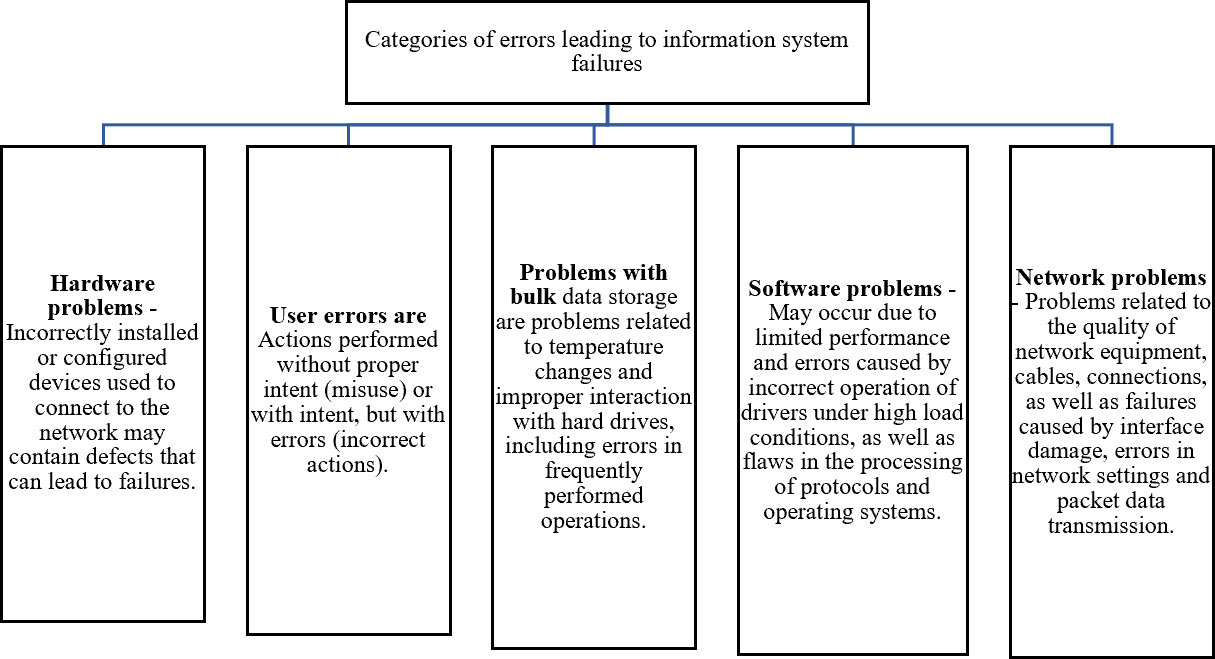
\includegraphics[width=0.8\textwidth]{assets/44}
	\caption*{}
\end{figure}

\textbf{Figure 2 - Errors that can lead to failures And}

In the framework of system-technical analysis, information systems are
considered as integrated structures consisting of interconnected and
interacting levels. The key elements of such systems are system and
application software, database management systems, as well as a set of
functions and services responsible for data transmission, storage and
processing (Figure 3).

\begin{figure}[H]
	\centering
	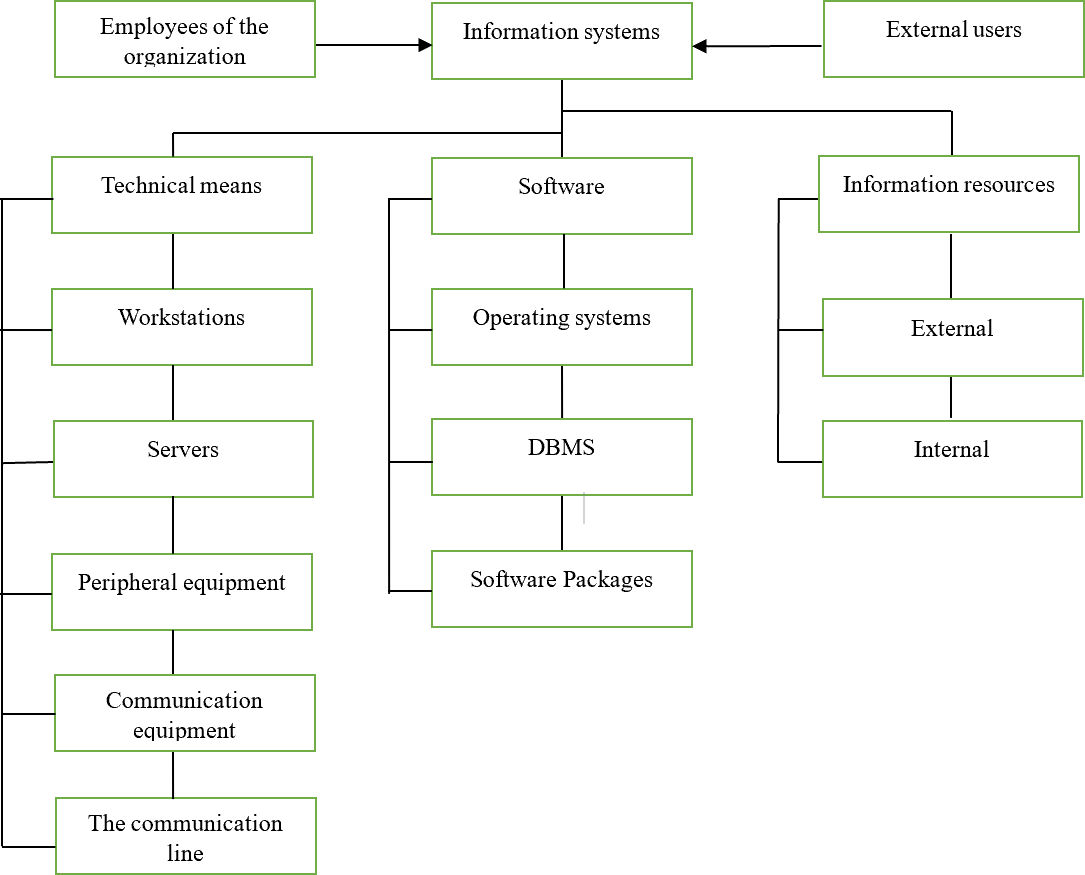
\includegraphics[width=0.8\textwidth]{assets/45}
	\caption*{}
\end{figure}

\textbf{Figure 3- Information systems}

When developing reliable and fault-tolerant information systems and
networks, significant attention is dedicated to minimizing the time and
resources required for the recovery and replacement of failed
components. In light of this, the application of various modeling
methods for selecting the optimal strategy for implementing backup
elements, considering potential failures, becomes a highly sought-after
approach.

The task of modeling and assessing the probabilities of failures in
information systems acquires particular relevance, allowing for the
identification of components that require modernization or replacement
with backups. For addressing this task, it is appropriate to use the
Markov chain methodology. This method is one of the most accessible and
effective mathematical tools for modeling various operations, including
failures in information systems, occurring as random processes.

Markov chains are an established mathematical tool for analyzing
problems with a probabilistic nature. Such a chain is represented in the
form of a graph, where vertices correspond to system states, and edges
reflect the intensity of transitions between these states. Using an
annotated graph, it is possible to determine the probabilities of the
system being in each of the states both over time and in stationary
conditions.

Before beginning modeling, initial parameters are defined, such as
possible states of failures specific to the analyzed information system,
and all potential connections between states are established in the form
of event flow intensities that effectuate the system\textquotesingle s
transitions from one state to another.

Then, based on the set parameters, one can proceed to create the model
using graph methodology, based on the principles of Markov chain theory.

In the context of the analyzed information system, a failure is
considered a stochastic process with a finite set of states, where
events occur individually rather than en masse. This indicates the
ordinariness of the studied model, which also assumes the absence of
aftereffects. This means that the number of events occurring in any
given time interval does not correlate with the number of events in any
other non-overlapping interval.

In the process of building the model to assess network fault tolerance,
it is assumed that a failure can occur at any level of its operation at
any given time, including the local level, the network environment
level, or the level of system\textquotesingle s critically significant
nodes (Figure 4).

\begin{figure}[H]
	\centering
	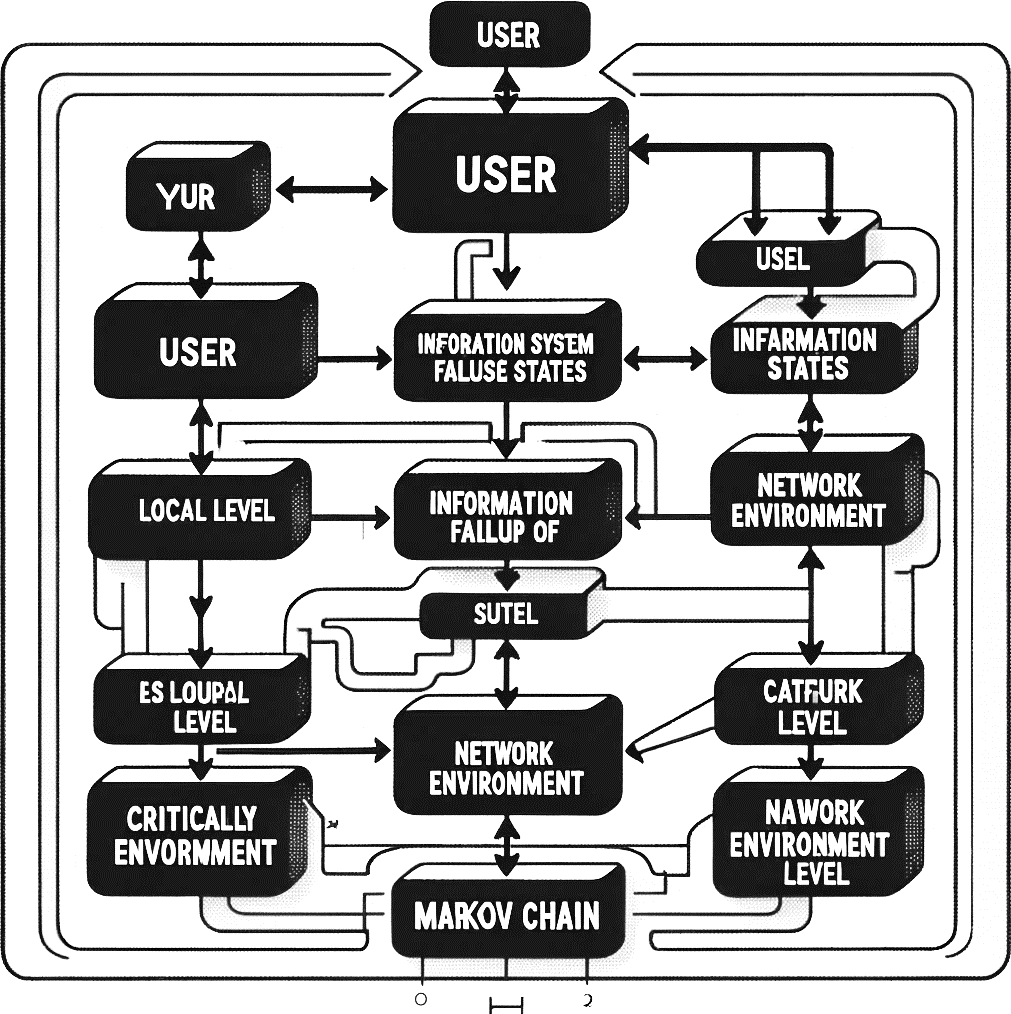
\includegraphics[width=0.8\textwidth]{assets/46}
	\caption*{}
\end{figure}

\textbf{Figure 4 - Schematic representation of the hierarchy of failure
states of an information system with}

\textbf{modeling based on Markov chains}

In the process of developing a model and evaluating the characteristics
of network fault tolerance, it is assumed that the information system at
certain points in time may experience a failure at one of the levels of
its functioning. These levels include: the local level, the network
environment level, and the critical node level. Within the framework of
modeling, it is assumed that the system can be in various failure
states, designated as Sij, where the index i indicates the level of
functioning (with three levels in this example), and the index j
classifies the type of failure (with five different types in this
example).

The initial state of the system is assumed to be trouble-free, with
fully functioning resources. All subsequent states differ from the
initial one and are characterized by non-standard operation of the
system in conditions of various failures.

Next, a graph of system states is constructed, which illustrates the
transitions from each possible failure state at the appropriate level to
a failure-free state, designated as S0. In this graph, the vertices
represent the possible states of the system, and the edges reflect the
intensity of transitions between these states, denoted as λi.

To quantify fault tolerance and failure probabilities in the network, a
mathematical model is formed based on the constructed graph of states.
This model is expressed through a system of differential or linear
algebraic equations, following the rule: on the left is the derivative
of the probability of a state in time, and on the right is the sum of
the products of the probabilities of states from which transitions to a
given state occur, based on the intensity of the corresponding streams
of events, minus the total intensity of the streams leading away from
this state, multiplied by the probability of this state.

To assess the level of fault tolerance and find the probabilities of
failures in the network according to a structured graph, we compile a
mathematical model in the form of a system of differential or linear
algebraic equations according to the following rule: on the left is the
derivative of the probability of the state, and on the right is the sum
of the products of the probabilities of those states from which the
arrows go to this state, based on the intensity of the corresponding
event flows, minus the total intensity of the flows leading from a given
state multiplied by the probability of a given state

To quantify the fault tolerance of the network and determine the
probability of failures, a mathematical model based on the constructed
graph of states is used. The model is presented in the form of a system
of differential or linear algebraic equations, which are formulated as
follows:

The left side of the equation contains the derivative of the probability
of finding the system in a given state in time, which corresponds to the
rate of change in the probability of this state.

The right side of the equation consists of two parts:

The first part includes the sum of the products of the probabilities of
previous states on the intensity of the streams of events that transfer
the system to this state. This reflects the contribution to the
probability of a state from all possible previous states.

The second part is the product of the probability of the current state
by the total intensity of the streams of events that bring the system
out of this state. This expresses the loss of probability due to
transitions to other states.

Thus, if we denote the probability of the \(S_{i}\) state as
\(P(S_{i})\) and the intensity of the transition from the \(S_{i}\)
state to the \(S_{j}\ \)state as \(\lambda_{ij}\), then for each
\(S_{i}\) state the equation will take the form:

\[\frac{dP(S_{i})}{dt} = \sum_{j \neq i}^{}{P(S_{j})}\lambda_{ji} - P(S_{i})\sum_{j \neq i}^{}\lambda_{ij}\]

where \(\frac{dP(S_{i})}{dt}\) - is the rate of change in the
probability of the \(S_{i}\) state over time, the first term sums up the
contributions from all possible transitions to the \(S_{i}\) state, and
the second term subtracts the probability of leaving the Si state to all
other states.

Solving this system of equations will allow us to find the probabilities
of all states of the system at any given time or in a stationary mode,
if we consider the long-term behavior of the system.

\textbf{Discussion.} In the framework of modern research, an analysis of
the fault tolerance of information systems (IS) using the theory of
Markov chains has been carried out. The central part of the work is the
construction of an IC failure graph, which describes the probabilistic
transitions between different states of the system, including states
characterizing various levels of functioning and types of failures.
Failure states in this context are divided into three main categories:
the local level, the network environment level and the level of critical
nodes, each of which, in turn, is associated with five types of
failures, covering hardware, system, application problems, as well as
failures of network devices and physical communication channels.

The study begins with determining the initial state of the system,
assuming its full functionality without any failures. The subsequent
analysis focuses on modeling the transitions of the system to failure
states and back, using a mathematical model based on Markov circuits.
This approach allows us to quantify the probabilities of each of the
possible states of the system over time, which is a key aspect in
studying and improving its fault tolerance.

In the course of the study, a system of differential and linear
algebraic equations was developed, which allows us to calculate the
dynamics of changes in the probabilities of system states based on the
intensities of event flows leading to failures or restoration of
functioning. The solution of this system of equations makes it possible
to predict the behavior of the system in various operating conditions
and under various failure scenarios.

One of the most important results of the work was the identification of
key factors affecting the level of fault tolerance of the information
system. In addition, the most vulnerable components and levels of
functioning of the IC were identified, for which the risk of failure is
maximum. This data can be used in the development of strategies to
improve the reliability and fault tolerance of systems, as well as in
planning measures to prevent failures or minimize their consequences.

\textbf{Results.} As part of the research, a mathematical model based on
Markov chains was developed and tested to analyze the fault tolerance of
information systems (IS). The model allowed us to estimate the
probabilities of transitions between different states of the system,
including normal operation and various failure levels associated with
the local level, the level of the network environment and the level of
critical nodes. The failure specification included hardware problems,
system failures, application problems, failures of network devices and
physical communication channels.

The main results of the study can be summarized as follows:

Quantification of the probabilities of states - the probabilities of
finding the system in each of the possible states were determined
depending on the time and operating conditions. This made it possible to
identify the most vulnerable components of the IC to failures and
evaluate the effectiveness of various strategies to increase fault
tolerance.

Identification of key fault tolerance factors - the study showed that
the intensity and probability of failures significantly depend on the
level of functioning of the system components and the type of possible
failures. Identifying these dependencies allows you to focus efforts on
eliminating the most significant vulnerabilities.

Analysis of the dynamics of changes in system states - the proposed
approach made it possible to trace how the probability of finding a
system in certain failure states changes over time, which contributes to
a better understanding of the recovery processes after failures and
planning preventive measures.

Development of recommendations to improve fault tolerance - based on the
results obtained, recommendations were formulated to improve the
architecture and configuration of information systems aimed at reducing
the likelihood of failures and minimizing their consequences.

Thus, the results of this study make a significant contribution to the
theory and practice of designing and operating fault-tolerant
information systems. The use of mathematical modeling based on Markov
chains allows for a more in-depth analysis of the processes taking place
in the IP and the development of effective risk management strategies
related to potential failures.

\textbf{References}

1.Nikscresht M. et al. Impact of selective implementation on soft error
detection through low-level re-execution //2021 IEEE Intl Conf on
Dependable, Autonomic and Secure Computing, Intl Conf on Pervasive
Intelligence and Computing, Intl Conf on Cloud and Big Data Computing,
Intl Conf on Cyber Science and Technology Congress
(DASC/PiCom/CBDCom/CyberSciTech). -- IEEE, 2021. - P. 112-117.

DOI:10.1109/DASC-PICom-CBDCom-CyberSciTech52372.2021.00031

2.Ijeh I. C. A collision-avoidance system for an electric vehicle: a
drive-by-wire technology initiative // SN Applied Sciences. -
2020.-Vol.2 (4)- P. 744.

DOI:10.1007/s42452-020-2383-2

3.Aponte-Moreno A., Restrepo-Calle F., Pedraza C. Using approximate
computing and selective hardening for the reduction of overheads in the
design of radiation-induced fault-tolerant systems // Electronics.
-2019.- Vol.8.(12) -P.1539. https://doi.org/10.3390/electronics8121539

4.Reghenzani F. et al. A mixed-criticality approach to fault tolerance:
integrating schedulability and failure requirements //2022 IEEE 28th
Real-Time and Embedded Technology and Applications Symposium
(RTAS).-IEEE.- 2022.- P. 27-39. DOI:10.1109/RTAS54340.2022.00011

5.Wu H., Guo R., Hu Y. FERNANDO: A software transient fault tolerance
approach for embedded systems based on redundant multi-threading // IEEE
Access.-2021.-Vol. 9.-P. 67154-67166.

DOI:10.1109/ACCESS.2021.3077190

6.Siddique A., Basu K., Hoque K. A. Exploring fault-energy trade-offs in
approximate DNN hardware accelerators // 2021 22nd International
Symposium on Quality Electronic Design (ISQED).-IEEE.- 2021.- P.
343-348. DOI:10.1109/ISQED51717.2021.9424345

7.Baloch N. K., Baig M. I., Daneshtalab M. Defender: A low overhead and
efficient fault-tolerant mechanism for reliable on-chip router // IEEE
Access.-2019.-Vol.7.- P.142843-142854.

DOI:~10.1109/ACCESS.2019.2944490

8.Isik M. et al. A design methodology for fault-tolerant computing using
astrocyte neural networks // Proceedings of the 19th ACM International
Conference on Computing Frontiers. -2022.- P.169-172.
DOI:10.1145/3528416.3530232

9.Cohen A. et al. Secure multi-source multicast // IEEE Transactions on
Communications. -- 2018. Vol. 67 (1).- P.708-723.
DOI:10.1109/TCOMM.2018.2870831

10.Pan J., Qian C., Ringerud M. Signed (group) diffie--hellman key
exchange with tight security // Journal of Cryptology.- 2022. --
Vol.35(4).- P. 26. https://doi.org/10.1007/s00145-022-09438-y

11.Rambo E. A., Shang Y., Ernst R. Providing integrity in real-time
networks-on-chip // IEEE Transactions on Very Large Scale Integration
(VLSI) Systems.-2019.- Vol.27.(8)- P. 1907-1920.

12.Gabillon A., Gallier R., Bruno E. Access controls for IoT networks //
SN Computer Science. -2020.-Vol.1(1).- P. 24.
DOI:10.1007/s42979-019-0022-z

13.Xu J. et al. Formalization and verification of Kafka messaging
mechanism using CSP // Computer Science and Information
Systems.-2023.-Vol.20(1).- P. 277-306

https://doi.org/10.2298/CSIS210707057X

14.Chia J., Chin J. J., Yip S. C. Digital signature schemes with strong
existential unforgeability //
F1000Research.-2021.DOI:10.12688/f1000research.72910.1

15.Cheu A., Yan C. Pure differential privacy from secure intermediaries
// arXiv preprint arXiv:2112.10032. -- 2021.
https://doi.org/10.48550/arXiv.2112.10032

16.Blazy O. et al. SAID: reshaping signal into an identity-based
asynchronous messaging protocol with authenticated ratcheting // 2019
IEEE European Symposium on Security and Privacy (EuroS\&P).
--IEEE.-2019.- P.294-309. DOI:10.1109/EuroSP.2019.00030

17. Shivpal Singh, Bhogendra Rao. Issues in design and development of
reliable configurable distributed checkout and launch system for mission
critical aero-space flight vehicles // International Journal of
Innovative Technology and Exploring Engineering (IJITEE).- 2020.-Vol. 9
(4S2)- P.77-81. DOI:~10.35940/ijitee.D1018.0394S220

18.Yoo A. et al. Fail-slow fault tolerance needs programming support //
Proceedings of the Workshop on Hot Topics in Operating Systems. -2021.-
P. 228-235.

19.Sahasrabudhe D., Berzins M., Schmidt J. Node failure resiliency for
Uintah without checkpointing // Concurrency and Computation: Practice
and Experience.- 2019.

https://doi.org/10.1002/cpe.5340

20.Zhao H. et al. Message‐sensing classified transmission scheme based
on mobile edge computing in the internet of vehicles // Software:
Practice and Experience. -2021.-Vol.51.(12) - P. 2501-2518.
DOI:10.1002/spe.2843

21.Kausar S. et al. Secure and efficient data transfer using spreading
and assimilation in MANET // Software: Practice and Experience.-2020.-
Vol.50 (11) -P.2095-2109. DOI:10.1002/spe.2782

22.Guo T. et al. Weakly secure symmetric multilevel diversity coding
//2019 IEEE Information Theory Workshop (ITW).
DOI:10.1109/ITW44776.2019.8989083

23.Stănescu D. et al. Cover processing-based steganographic model with
improved security // Acta Polytechnica Hungarica.- 2019.-Vol.16.(1)-
P.227-246.

\emph{\textbf{Information about the authors}}

Kaiupov Ye. K. \textbf{-} doctoral student, L. N. Gumilev Eurasian
National University,Astana, Kazakhstan,

е-mail: yerik.kai@gmail.com;

Mukanova А. - PhD, аssoc. professor of the Astana International
University, Astana, Kazakhstan, е-mail: asiserikovna@gmail.com;

Nazyrova A. - senior lecturer of the Astana International University,
Astana, Kazakhstan,

е-mail: ayzhan.nazyrova@gmail.com;

Tashtay B. -senior lecturer of the L. N. Gumilyov Eurasian National
University, Astana, Kazakhstan, е-mail: 93bahti93@gmail.com;

Toleubekov Т. - is a senior lecturer at the Eurasian National
University. L.N. Gumilyov,Astana, Kazakhstan, е-mail:
toleubekovtm@gmail.com

\emph{\textbf{Сведения об авторах}}

Кайупов Е.К. \textbf{-}докторант Евразийского национального университета
им. Л. Н. Гумилева, Астана, Казахстан, е-mail: yerik.kai@gmail.com;

Муканова А. - PhD, доцент Международного университета Астаны, Астана,
Казахстан, е-mail: asiserikovna@gmail.com;

Назырова А. - старший преподаватель Международного университета Астаны,
Астана, Казахстан, е-mail: ayzhan.nazyrova@gmail.com;

Таштай Б\textbf{.} -старший преподаватель Евразийского национального
университета имени Л.Н. Гумилева, Астана, Казахстан, е-mail:
93bahti93@gmail.com;

Толеубеков Т.-старший преподаватель Евразийского национального
университета им. Л.Н. Гумилева, Астана, Казахстан,
е-mail:toleubekovtm@gmail.com

.

МРНТИ 20.15.05

\textbf{АНАЛИЗ РАСШИРЕННЫХ ВОЗМОЖНОСТЕЙ СИСТЕМЫ SIEM ЧЕРЕЗ ИНТЕГРАЦИЮ С
IBM QRADAR}

\textbf{\textsuperscript{1}Ж. Бидахмет, \textsuperscript{1}Г.З.
Зиятбекова, \textsuperscript{1}С.К. Заманова, \textsuperscript{2}Ж.Ж.
Кожамкулова,}

\textbf{\textsuperscript{3}А.К. Адильбекова, \textsuperscript{1}С.М.
Жаксыбай}

\textsuperscript{2}Казахский национальный университет имени аль-Фараби,
Алматы, Казахстан,

\textsuperscript{2}НАО АУЭС имени Г. Даукеева, Алматы, Казахстан,

\textsuperscript{3}Казахский университет международных отношений и
мировых языков

имени Абылай хана, Алматы, Казахстан,

е-mail: zhaksybaysanzhar@gmail.com

В данной статье рассматриваются важные аспекты SIEM-технологии, роли в
кибербезопасности и ее компонентов, обсуждаются ключевая роль
SIEM-системы в современном мире информационных технологий, а также
рассмотрены основные компоненты SIEM-системы, включая сборщики данных,
системы корреляции, дэшборды и отчеты. Представлен код, являющийся
частью разработки, предназначенной для мониторинга сетевого трафика и
обнаружения потенциальных угроз, таких как DDoS-атаки. Основные
использованные технологии и методы описаны ниже.

\textbf{Ключевые слова:} SIEM, IBM QRadar, DDoS-атака, информационная
безопасность, кибербезопасность, мониторинг, угроза.

\textbf{IBM QRADAR ИНТЕГРАЦИЯСЫ АРҚЫЛЫ SIEM ЖҮЙЕСІНІҢ КЕҢЕЙТІЛГЕН
МҮМКІНДІКТЕРІН ТАЛДАУ}

\textbf{\textsuperscript{1}Ж. Бидахмет, \textsuperscript{1}Г.З.
Зиятбекова, \textsuperscript{1}С.К. Заманова, \textsuperscript{2}Ж.Ж.
Кожамкулова,}

\textbf{\textsuperscript{3}А.К. Адильбекова, \textsuperscript{1}С.М.
Жаксыбай}

\textsuperscript{1}әл-Фараби атындағы Қазақ ұлттық университеті, Алматы,
Қазақстан,

\textsuperscript{2}Г. Даукеев атындағы КЕАҚ АЭжБУ, Алматы, Қазақстан,

\textsuperscript{3}Абылай хан атындағы ҚазХҚжӘТУ, Алматы, Қазақстан,

е-mail: zhaksybaysanzhar@gmail.com

Бұл мақалада SIEM технологиясының маңызды аспектілері, оның
киберқауіпсіздіктегі рөлі мен құрамдас бөліктері қарастырылады,
ақпараттық технологиялардың заманауи әлеміндегі SIEM жүйесінің негізгі
маңыздылығы талқыланады, сонымен қатар, SIEM жүйесінің негізгі құрамдас
бөліктері, соның ішінде дерек жинаушылар, корреляциялық жүйелер, бақылау
тақталары және есептер қарастырылады. Ұсынылған код желілік трафикті
бақылауға және DDoS шабуылдары сияқты ықтимал қауіптерді анықтауға
арналған әзірлеменің бөлігі болып табылады. Қолданылатын негізгі
технологиялар мен әдістер төменде сипатталған.

\textbf{Түйін сөздер:} SIEM, IBM QRadar, DDoS шабуылы, ақпараттық
қауіпсіздік, киберқауіпсіздік, мониторинг, қауіп.

\textbf{ANALYZE SIEM SYSTEM ADVANCED FEATURES THROUGH INTEGRATION WITH
IBM QRADAR}

\textbf{\textsuperscript{1}Zh. Bydakhmet, \textsuperscript{1}G.Z.
Ziyatbekova, \textsuperscript{1}S.K. Zamanova, \textsuperscript{2}Zh.Zh.
Kozhamkulova,}

\textbf{\textsuperscript{3}A.K. Adilbekova, \textsuperscript{1}S.M.
Zhaksybay}

\textsuperscript{1}Al-Farabi Kazakh National University, Almaty,
Kazakhstan,

\textsuperscript{2}Non-profit joint-stock company \textbf{``}Almaty
University of Power Engineering and Telecommunications after Gumarbek
Daukeev'' Almaty, Kazakhstan,

\textsuperscript{3}Kazakh Ablaikhan university of international
relations and world languages,

Almaty, Kazakhstan,

е-mail: zhaksybaysanzhar@gmail.com

This article discusses important aspects of SIEM technology, the role in
cybersecurity and its components, discusses the key role of the SIEM
system in the modern world of information technology, and examines the
main components of the SIEM system, including data collectors,
correlation systems, dashboards and reports. The code is presented,
which is part of a development designed to monitor network traffic and
detect potential threats such as DDoS attacks. The main technologies and
methods used are described below.

\textbf{Keywords:} SIEM, IBM QRadar, DDoS attack, information security,
cybersecurity, monitoring, threat.

\textbf{Введение.} Системы управления информацией и событиями
безопасности (SIEM -- Security information and event management) начали
свое развитие в конце 1990-х -- начале 2000-х годов из простых систем
лог-менеджмента. Эти системы первоначально были созданы для сбора,
агрегирования и хранения лог-файлов от различных систем и устройств в
централизованном хранилище. Основной целью было обеспечить удобный
доступ к логам для целей аудита и устранения неисправностей. Со временем
возникла потребность в более продвинутом анализе данных для обнаружения
и предотвращения инцидентов безопасности.

\emph{Развитие функциональности: Корреляция и аналитика.} Как
развивались технологии и увеличивалось количество киберугроз, стало
очевидно, что простого сбора и хранения логов недостаточно. В ответ на
это появились системы, способные не только собирать данные, но и
анализировать их на предмет аномалий и угроз. Так родились первые
SIEM-системы, которые начали использовать правила для корреляции событий
и алертов, позволяя IT-специалистам и аналитикам безопасности более
эффективно реагировать на инциденты.

\emph{Внедрение технологий машинного обучения и больших данных}. С
развитием технологий больших данных и машинного обучения современные
SIEM-системы стали значительно мощнее. Они начали предлагать не только
реактивный, но и проактивный подход к безопасности. Это включало
поведенческий анализ и аналитику в реальном времени, что позволило
обнаруживать даже сложные угрозы, маскирующиеся под обыденную активность
в сети {[}1-2{]}.

\emph{Роль IBM QRadar в эволюции SIEM.} IBM QRadar является одним из
лидеров в области SIEM. Он был разработан для предоставления
комплексного решения по управлению сетевой безопасностью, которое
интегрирует сбор логов, мониторинг событий, их корреляцию и аналитику.
QRadar использует сложные алгоритмы для анализа и корреляции данных, что
позволяет обнаруживать угрозы более эффективно и в более ранние стадии,
чем традиционные системы. Эта эволюция отражает не только технический
прогресс, но и изменения в подходах к обеспечению безопасности, делая
современные SIEM-системы более адаптивными и интеллектуальными {[}3{]}.

\emph{Основные технологии и методы обнаружения угроз.} \emph{Примеры и
кейс-стади.} Примером сложной угрозы может служить атака через
беспроводные сети, где злоумышленники используют сетевые запросы для
распространения вредоносного ПО в пределах корпоративной сети. В таких
случаях SIEM системы, оснащенные инструментами для глубокого анализа
сетевого трафика и поведенческого мониторинга, могут быстрее обнаружить
и нейтрализовать угрозу.

Сложность и разнообразие современных киберугроз требуют от SIEM систем
не только быстрого реагирования, но и глубокого понимания контекста
каждой угрозы. Развитие технологий, таких как машинное обучение и
искусственный интеллект, помогает современным SIEM системам, включая IBM
QRadar, эффективно справляться с этими вызовами, предоставляя более
мощные и умные инструменты для защиты цифровых активов организаций
{[}4{]}.

\emph{Основные технологии.} \emph{Flask:} это легковесный веб-фреймворк
на языке Python, предназначенный для создания веб-приложений. В данном
контексте он используется для создания веб-интерфейса для мониторинга
сетевого трафика.

\emph{Scapy:} это мощная библиотека Python, которая позволяет
интерактивно работать с сетевыми пакетами. В коде используются модули
\emph{sniff, IP}, и \emph{TCP} из Scapy для перехвата и анализа сетевого
трафика.

\emph{Subprocess:} Модуль Python, используемый для запуска новых
приложений или программ, которые могут выполняться параллельно с
Python-скриптом.

\emph{Logging:} Модуль Python для логирования событий. В данном коде он
настраивается для сохранения записей о сетевом трафике в файл
\emph{network\_traffic.log}.

\emph{Nmap:} Инструмент для исследования сети и аудита безопасности.
Хотя он не показан в действии в представленном фрагменте кода, его можно
использовать для сканирования сети на наличие уязвимых портов {[}5-6{]}.

\textbf{Материалы и методы.} \emph{Сбор данных:} Используя Scapy,
система перехватывает сетевой трафик и собирает данные о пакетах,
передаваемых через сеть.

\emph{Анализ портов:} В коде определены уязвимые порты
(\emph{vulnerable\_ports}), которые могут подвергаться сканированию или
атакам. Система может анализировать трафик на эти порты для обнаружения
подозрительной активности.

\emph{Обнаружение аномалий:} Установлен порог
(\emph{anomalous\_traffic\_threshold}) для обнаружения аномального
трафика. Если объем трафика превышает этот порог, система может
генерировать предупреждение о возможной аномалии.

\emph{DDoS обнаружение:} Порог (\emph{ddos\_threshold}) устанавливается
для обнаружения DDoS-атак. Это сделано для мониторинга необычно высокого
трафика, который может указывать на DDoS.

Использование этих технологий и методов в совокупности позволяет создать
систему, способную эффективно мониторить сетевой трафик и предупреждать
о потенциальных угрозах в реальном времени. Такая система становится
важной частью защитного механизма в контексте кибербезопасности,
дополняя возможности традиционных SIEM систем и повышая общую
защищенность сетевой инфраструктуры.

Практическое применение разработки: интеграция сетевого мониторинга и
анализа {[}7-8{]}.

\textbf{Результаты и обсуждение.} \emph{Описание кода.} Код системы
(Рис. 1-4) начинается с импорта необходимых библиотек:

\begin{figure}[H]
	\centering
	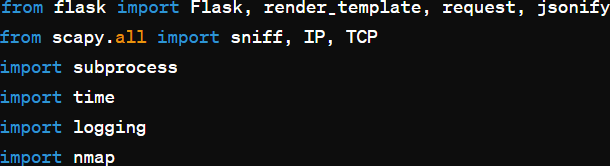
\includegraphics[width=0.8\textwidth]{assets/47}
	\caption*{}
\end{figure}

\textbf{Рис. 1 -- Импорт необходимых библиотек}

Затем, настраивается базовая конфигурация логирования и создается
экземпляр Flask-приложения:

\begin{figure}[H]
	\centering
	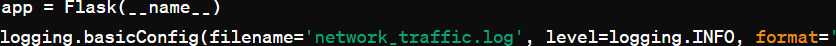
\includegraphics[width=0.8\textwidth]{assets/48}
	\caption*{}
\end{figure}

\textbf{Рис. 2 -- Flask-приложение}

С помощью Scapy осуществляется захват пакетов и анализ сетевого трафика.
Каждый пакет обрабатывается функцией packet\_handler, которая извлекает
важные данные и хранит их в словаре:

\begin{figure}[H]
	\centering
	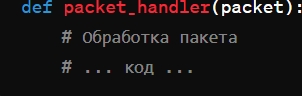
\includegraphics[width=0.8\textwidth]{assets/49}
	\caption*{}
\end{figure}

\textbf{Рис. 3 - Анализ сетевого трафика}

В коде реализованы механизмы для определения аномального трафика и
обнаружения DDoS-атаки, а также функции для блокировки IP-адресов,
подозрительных в сканировании портов.

Примеры использования. Возьмем для примера функцию обнаружения
аномального трафика:

\begin{figure}[H]
	\centering
	\includegraphics[width=0.8\textwidth]{assets/50}
	\caption*{}
\end{figure}

\textbf{Рис. 4 - Функция обнаружения аномального трафика}

Этот фрагмент кода проверяет, превышает ли количество трафика для пары
IP-адресов установленный порог, и в случае обнаружения аномалии отмечает
соответствующий IP-адрес как аномальный.

Интеграция с Nmap для сканирования уязвимостей. Кроме того, мы
использовали

\emph{Цветовая индикация угроз.} Для улучшения восприятия информации и
скорости реагирования таблицы используют цветовую индикацию для
различных типов угроз (Рис. 5-7):

- Красный цвет выделяет уязвимые порты и потенциальные DDoS-атаки.

- Желтый цвет указывает на аномальный трафик.

- Зеленый цвет предупреждает о сканировании портов.

\begin{figure}[H]
	\centering
	\includegraphics[width=0.8\textwidth]{assets/51}
	\caption*{}
\end{figure}

\textbf{Рис. 5 - Цветовая индикация угроз}

\begin{figure}[H]
	\centering
	\includegraphics[width=0.8\textwidth]{assets/52}
	\caption*{}
\end{figure}\begin{figure}[H]
	\centering
	\includegraphics[width=0.8\textwidth]{assets/52}
	\caption*{}
\end{figure}

\textbf{Рис. 6 - Исходящий трафик Рис. 7 - Входящий трафик}

\emph{Обнаружение и предотвращение сканирования портов. Описание кейса:}
Средняя компания ABC, работающая в сфере финансовых услуг, столкнулась с
увеличением числа попыток несанкционированного сканирования портов в их
сети, что создавало потенциальные угрозы безопасности. Для защиты от
таких атак компания внедрила нашу систему мониторинга. Система
мониторинга непрерывно анализировала сетевой трафик и применяла
алгоритмы обнаружения сканирования портов для выявления подозрительной
активности. При обнаружении таких попыток система автоматически
блокировала исходящие запросы с подозрительных IP-адресов.

\emph{Эффективное обнаружение угроз:} Система успешно выявила и
предотвратила ряд попыток сканирования портов, минимизируя риски
нарушения безопасности и сокращая время необходимое для реагирования на
инциденты.

\emph{Повышение защищенности сети:} благодаря реакции в реальном времени
на угрозы, компания смогла улучшить общий уровень безопасности своей
сети и защитить конфиденциальные данные клиентов.

\emph{Сокращение операционных затрат:} Уменьшение количества атак на
сеть привело к сокращению времени, затрачиваемого на расследование
инцидентов и восстановление сервисов.

Рассмотренные кейс-стади являются лишь двумя примерами успешного
применения системы мониторинга сетевого трафика, разработанной нами. Эти
кейсы подчеркивают значимость эффективного мониторинга и оперативного
реагирования на угрозы для обеспечения безопасности и надежности
корпоративных сетей.

\emph{Тенденции и прогнозы в области SIEM, исследование текущих
тенденций.} Системы управления информационной безопасностью (SIEM)
продолжают развиваться, приспосабливаясь к новым вызовам и угрозам в
области кибербезопасности. Некоторые текущие тенденции в этой области
включают:

\emph{Облачные решения:} Возрастающая потребность в масштабируемых и
гибких решениях подталкивает компании к переходу от локальных SIEM
систем к облачным платформам, что позволяет более эффективно управлять
растущим объемом данных.

\emph{Искусственный интеллект и машинное обучение:} Использование
алгоритмов машинного обучения и искусственного интеллекта становится все
более распространенным в SIEM системах для более точного обнаружения и
анализа угроз.

\emph{Расширенный анализ данных:} Компании все больше осознают ценность
данных о безопасности не только для реагирования на инциденты, но и для
принятия стратегических решений в области кибербезопасности.

\emph{Будущие инновации.} В будущем можно ожидать дальнейшего развития
SIEM систем в следующих направлениях:

\emph{Автоматизация и оркестрация:} Развитие автоматизированных
процессов обнаружения и реагирования на угрозы позволит компаниям
сократить время реагирования на инциденты и улучшить эффективность своих
кибербезопасных операций.

\emph{Усиление аналитики:} Внедрение более продвинутых методов аналитики
данных, таких как анализ поведения пользователей и контекстной
информации, позволит более точно выявлять потенциальные угрозы.

\emph{Интеграция с другими технологиями:} SIEM системы будут все более
интегрироваться с другими технологиями кибербезопасности, такими как EDR
(Endpoint Detection and Response) и SOAR (Security Orchestration,
Automation, and Response), для обеспечения более полного и
согласованного подхода к безопасности {[}9{]}.

\emph{Вклад разработки в будущее индустрии.} Разработка представляет
собой важный шаг в направлении инновационных решений в области SIEM.
Таким образом продукт может формировать будущее систем SIEM:

\emph{Расширенные алгоритмы обнаружения:} Система предлагает расширенные
алгоритмы обнаружения аномального трафика, DDoS-атак и сканирования
портов, что позволяет более точно выявлять угрозы и снижать ложные
срабатывания.

\emph{Интеграция с облачными технологиями:} Интеграция системы с
облачными технологиями позволяет клиентам быстрее и легче масштабировать
свои кибербезопасные операции в соответствии с их потребностями.

\emph{Повышение эффективности операций:} Продукт обеспечивает более
быструю реакцию на угрозы благодаря автоматизации и оптимизации
процессов обнаружения и реагирования, что в конечном итоге позволяет
нашим клиентам сэкономить время и ресурсы.

\emph{Снижение времени реагирования:} благодаря системе мониторинга,
корпорация смогла оперативно реагировать на DDoS-атаки, минимизируя
временные простои и потери до минимума.

\emph{Увеличение доступности сервисов:} Применение системы позволило
значительно увеличить доступность онлайн-сервисов корпорации, повысив
удовлетворенность клиентов.

\emph{Экономические выгоды:} Подсчет экономических потерь, связанных с
DDoS-атаками, показал существенное сокращение убытков после внедрения
системы мониторинга {[}10{]}.

\emph{Взгляд в будущее.} Исследование показывает, что будущее SIEM
система будет определяться инновациями в области облачных технологий,
искусственного интеллекта и автоматизации процессов. Разработка играет
ключевую роль в этом развитии, предлагая расширенные алгоритмы
обнаружения, интеграцию с облачными платформами и повышение
эффективности операций кибербезопасности.

\textbf{Выводы.} В заключении отражается текущие тенденции в области
SIEM, но и указывает на будущее направление развития этой индустрии.
Можно сказать, что вклад способствует укреплению кибербезопасности и
защите информационных ресурсов как для корпоративных клиентов, так и для
конечных пользователей.

Разработка не только предлагает инновационные технологические
возможности, но и способствует укреплению общей безопасности
информационных систем, что делает ее ключевым игроком в будущем развитии
индустрии SIEM. В статье рассмотрена эволюция систем управления
информационной безопасностью (SIEM) от простых лог-систем до современных
аналитических платформ. Обсуждена роль системы IBM QRadar в индустрии и
выявлены текущие вызовы, с которыми сталкиваются SIEM системы, включая
объем данных, сложность угроз и недостатки текущих решений.

\textbf{Литература}

1.David R. Miller,~ Shon Harris,~ Allen Harper,~ Stephen VanDyke,~ Chris
Blask Security Information and Event Management (SIEM) Implementation//
Mcgraw-hill , 2010.- 464 P. ISBN 978-0-07-170108-2

2.Vitalii Varkentin, Kseniia Nikolskaia. Особенности создания наборов
данных для обучения систем обнаружения вторжений, основанных на методах
машинного обучения. Сборник материалов конференции. СПб.: Изд-во СПбГЭТУ
«ЛЭТИ», 2019.- Т.1.- С. 141-143.

3.Joseph Muniz, Gary McIntyre, and Nadhem AlFardan. Security Operations
Center: Building, Operating, and Maintaining Your SOC Paperback// Gisco
Press.- 448 p. ISBN 978-0134052014

4.Richard Bejtlich. The Practice of Network Security Monitoring:
Understanding Incident Detection and Response, 2013. -376 р. ISBN
101-59327-509-9

https://terrorgum.com/tfox/books/practiceofnetworksecuritymonitoring.pdf

5.Gerardus Blokdyk. Security Information and Event Management (SIEM) --
A Complete Guide// ~5STARCooks, 2020.- 320 p. ISBN10:0655914668, ISBN
13:978-0655914662

https://www.amazon.com/Security-Information-Event-Management-Complete/dp/0655914668

6.Gustavo González-Granadillo, Susana González-Zarzosa and Rodrigo Diaz.
Security Information and Event Management (SIEM): Analysis, Trends, and
Usage in Critical Infrastructures// Sensors, 2021.- Vol.21(14), 4759.
https://doi.org/10.3390/s21144759

7.Rahman Ali, Asmat Ali, Farkhund Iqbal, Mohammed Hussain and Farhan
Ullah. Deep Learning Methods for Malware and Intrusion Detection: A
Systematic Literature Review// Security and Communication Networks,
2022.- Vol.22.- 31 р. https://doi.org/10.1155/2022/2959222

8.Yanli Shao, Yang Lu, Dan Wei, Jinglong Fang, Feiwei Qin and Bin Chen.
Malicious Code Classification Method Based on Deep Residual Network and
Hybrid Attention Mechanism for Edge Security// Wireless Communications
and Mobile Computing,2022.- Vol.2022.- 19 p.

DOI https://doi.org/10.1155/2022/3301718

9.Смирнов А.И. Глобальная безопасность: инновационные методы анализа
конфликтов. -- М.: Знание, 2013. -- 278 с.

10.Жаксыбай С.М. Управление событиями информационной безопасности с
помощью SIEM-системы// Интелектуальные технологии на транспорте,2023.-№
S1 (спецвыпуск).- С. 66- 69. https://ivs.pgups.ru/events/mmis-2023

\textbf{References}

1.David R. Miller,~ Shon Harris,~ Allen Harper,~ Stephen VanDyke,~ Chris
Blask Security Information and Event Management (SIEM) Implementation//
Mcgraw-hill , 2010.- 464 P. ISBN 978-0-07-170108-2

2.Vitalii Varkentin, Kseniia Nikolskaia. Osobennosti sozdanija naborov
dannyh dlja obuchenija sistem obnaruzhenija vtorzhenij, osnovannyh na
metodah mashinnogo obuchenija. Sbornik materialov konferencii. SPb.:
Izd-vo SPbGJeTU «LJeTI», 2019.- T.1.- S. 141-143.{[}in Russian{]}

3.Joseph Muniz, Gary McIntyre, and Nadhem AlFardan. Security Operations
Center: Building, Operating, and Maintaining Your SOC Paperback// Gisco
Press.- 448 p. ISBN 978-0134052014

4.Richard Bejtlich. The Practice of Network Security Monitoring:
Understanding Incident Detection and Response, 2013. -376 р. ISBN
101-59327-509-9

https://terrorgum.com/tfox/books/practiceofnetworksecuritymonitoring.pdf

5.Gerardus Blokdyk. Security Information and Event Management (SIEM) --
A Complete Guide// ~5STARCooks, 2020.- 320 p. ISBN10:0655914668, ISBN
13:978-0655914662

https://www.amazon.com/Security-Information-Event-Management-Complete/dp/0655914668

6.Gustavo González-Granadillo, Susana González-Zarzosa and Rodrigo Diaz.
Security Information and Event Management (SIEM): Analysis, Trends, and
Usage in Critical Infrastructures// Sensors, 2021.- Vol.21(14), 4759.
https://doi.org/10.3390/s21144759

7.Rahman Ali, Asmat Ali, Farkhund Iqbal, Mohammed Hussain and Farhan
Ullah. Deep Learning Methods for Malware and Intrusion Detection: A
Systematic Literature Review// Security and Communication Networks,
2022.- Vol.22.- 31 р. https://doi.org/10.1155/2022/2959222

8.Yanli Shao, Yang Lu, Dan Wei, Jinglong Fang, Feiwei Qin and Bin Chen.
Malicious Code Classification Method Based on Deep Residual Network and
Hybrid Attention Mechanism for Edge Security// Wireless Communications
and Mobile Computing,2022.- Vol.2022.- 19 p.

DOI https://doi.org/10.1155/2022/3301718

9.Smirnov A.I. Global\textquotesingle naja bezopasnost\textquotesingle:
innovacionnye metody analiza konfliktov. -- M.: Znanie, 2013. -- 278 s.

10.Zhaksybaj S.M. Upravlenie sobytijami informacionnoj bezopasnosti s
pomoshh\textquotesingle ju SIEM-sistemy//
Intelektual\textquotesingle nye tehnologii na transporte,2023.-№ S1
(specvypusk).- S. 66- 69

https://ivs.pgups.ru/events/mmis-2023

\emph{\textbf{Сведения об авторах}}

Бидахмет Ж.-PhD, и.о. доцента Казахского национального университета им.
аль-Фараби, Алматы, Казахстан, e-mail: bidakhmetzhanar@gmail.com;

Зиятбекова Г.З.- PhD, и.о. доцента Казахского национального университета
им. аль-Фараби; автор-корреспондент, Алматы, Казахстан, e-mail:
ziyatbekova1@gmail.com;

Заманова С. К. -магистр технических наук, старший преподаватель
Казахского национального университета им. аль-Фараби, Алматы, Казахстан,
e-mail: zamanova.saule@gmail.com;

Кожамкулова Ж.Ж.- PhD, доцент, АУЭС им. Г. Даукеева, Алматы, Казахстан,
e-mail: zh.kozhamkulova@aues.kz;

Адильбекова А.К.-преподаватель Казахского университета международных
отношений и мировых языков им. Абылай хана, Алматы, Казахстан, e-mail:
adilbekova.a.k@mail.ru;

Жақсыбай С.М.-магистрант Казахского национального университета им.
аль-Фараби, Алматы, Казахстан, e-mail: zhaksybaysanzhar@gmail.com

\emph{\textbf{Information about the authors}}

B.Zhanar - PhD, аcting Associate professor Al-Farabi Kazakh National
University, Almaty, Kazakhstan, e-mail: bidakhmetzhanar@gmail.com;

G.Ziyatbekova - PhD, Acting Associate Professor Al-Farabi Kazakh
National University, Almaty, Kazakhstan, Corresponding author, e-mail:
ziyatbekova1@gmail.com;

S.Zamanova -Master of Technical Sciences, Senior Lecturer, Al-Farabi
Kazakh National University, Almaty, Kazakhstan, e-mail:
zamanova.saule@gmail.com;

Zh. Kozhamkulova- PhD, Associate Professor AUPET, Non-profit joint-stock
company ``Almaty University of Power Engineering and Telecommunications
after Gumarbek Daukeev'', Almaty, Kazakhstan, e-mail:
zh.kozhamkulova@aues.kz;

A.Adilbekova -Teacher Kazakh Ablai khan university of international
relations and world languages Ablaikhan, Almaty, Kazakhstan, e-mail:
adilbekova.a.k@mail.ru;

S.Zhaksybai - graduate student at Al-Farabi Kazakh National University,
Almaty, Kazakhstan, e-mail: zhaksybaysanzhar@gmail.com

МРНТИ 20.15.05

\textbf{РАЗВЕРТЫВАНИЕ КОНТЕЙНЕРНЫХ ПРИЛОЖЕНИЙ С ПОМОЩЬЮ МАШИННОГО
ОБУЧЕНИЯ: ОБЗОР И АНАЛИЗ}

\textbf{\textsuperscript{1,2}Л.Т. Кусепова, \textsuperscript{1}А.Б.
Оспанова, \textsuperscript{1,2}А.Е. Назырова, \textsuperscript{2}Г.Т.
Кусепова}

\textsuperscript{1}Международный университет Астана, Астана, Казахстан,

\textsuperscript{2}Евразийский национальный университет им. Л.Н.
Гумилева, Астана, Казахстан,

e-mail: lazzatk@mail.ru

В связи с динамическим развитием и растущей сложностью систем необходимо
постоянно выполнять поиск новых методов управления сервисами в облачных
вычислениях. Следовательно технологии контейнеризации помогают легко
развертывать приложения, управлять и распределять ресурсы облачных
провайдеров, тем самым масштабируя их, обеспечивать переносимость данных
и изоляцию приложений и их зависимостей. Однако с ростом сложности
инфраструктуры и данных возникают новые вызовы, такие как обеспечение
непрерывной работы сервисов, оптимизации ресурсов, балансировки
нагрузки, производительности систем. Для решения множеств проблем,
возникающих в контексте развертывания и управления контейнерными
приложениями, становится необходимым применение машинного обучения.
Интеграция технологии контейнеризации и машинного обучения позволяет
адаптироваться к изменяющимся условиям, оптимизировать использование
ресурсов и обеспечивать непрерывную работу системы. В статье представлен
обзор популярных методов машинного обучения и их применение в контексте
контейнерных технологий, была представлена эталонная архитектура
оркестровки контейнеров на основании машинного обучения и их эволюция, а
также были исследованы контейнеры и оркестраторы, такие как Kubernetes,
Docker, Prefect, Nomad, Red Hat OpenShift Service on AWS, Amazon Elastic
Container Service (ECS), Google Kubernetes Engine, Azure Kubernetes
Service. Методы машинного обучения могут быть использованы для
прогнозирования потребления ресурсов, адаптации к потребностям,
предсказания временных интервалов для управления кластерами контейнеров,
а также для анализа поведения рабочей нагрузки на основании прошлых
данных.

\textbf{Ключевые слова:} контейнерные технологии, оркестровка
контейнеров, машинное обучение, облачные вычисления, предоставление
ресурсов

\textbf{КОНТЕЙНЕРЛІК ҚОСЫМШАЛАРДЫ МАШИНАЛЫҚ ОҚЫТУ АРҚЫЛЫ ЖҮЗЕГЕ АСЫРУ:
ШОЛУ ЖӘНЕ ТАЛДАУ}

\textbf{\textsuperscript{1,2}Л.Т. Кусепова, \textsuperscript{1}А.Б.
Оспанова, \textsuperscript{1,2}А.Е. Назырова, Г.Т.
Кусепова\textsuperscript{2}}

\textsuperscript{1}Астана халықаралық университеті, Астана, Қазақстан,

\textsuperscript{2}Л.Н. Гумилев атындағы Еуразия ұлттық университеті,
Астана, Қазақстан,

e-mail: lazzatk@mail.ru

Жүйелердің динамикалық дамуы мен күрделілігінің артуына байланысты
бұлтты есептеулерде қызметтерді басқарудың жаңа әдістерін үнемі
іздестіріп отыру қажет. Сәйкесінше контейнерлік технологиялар
қолданбаларды оңай орналастыруға, бұлттық провайдер ресурстарын
басқаруға және үлестіруге көмектеседі, осылайша оларды масштабтайды,
деректердің тасымалдануын қамтамасыз етеді және қосымшалар мен олардың
тәуелділіктерін оқшаулайды. Дегенмен, инфрақұрылым мен деректердің
күрделене түсуіне байланысты қызметтердің үздіксіз жұмысын қамтамасыз
ету, ресурстарды оңтайландыру, жүктемені теңестіру және жүйе өнімділігі
сияқты жаңа міндеттер туындайды. Контейнерлік қосымшаларды орналастыру
және басқару контекстінде туындайтын көптеген мәселелерді шешу үшін
машиналық оқытуды пайдалану қажет болады. Контейнерлеу технологиясы мен
машиналық оқытудың интеграциясы өзгермелі жағдайларға бейімделуге,
ресурстарды пайдалануды оңтайландыруға және жүйенің үздіксіз жұмысын
қамтамасыз етуге мүмкіндік береді. Мақалада танымал машиналық оқыту
әдістеріне шолу және оларды контейнерлік технологиялар контекстінде
пайдалану, машиналық оқыту және олардың эволюциясы негізінде
контейнерлік оркестрлеудің анықтамалық архитектурасы ұсынылған, сонымен
қатар Kubernetes, Docker, Prefect, Nomad, Red Hat OpenShift Service on
AWS, Amazon Elastic Container Service (ECS), Google Kubernetes Engine,
Azure Kubernetes Service сияқты контейнерлер мен оркестраторлар
зерттелген. Машиналық оқыту әдістерін ресурстарды тұтынуды болжау,
сұранысқа бейімделу, контейнерлік кластерлерді басқару уақытын болжау
және тарихи деректер негізінде жұмыс жүктемесінің әрекетін талдау үшін
пайдалануға болады.

\textbf{Түйін сөздер:} контейнерлік технологиялар, контейнерлерді
оркестрлеу, машиналық оқыту, бұлтты есептеулер, ресурстарды ұсыну

\textbf{DEPLOYING CONTAINER APPLICATIONS THROUGH MACHINE LEARNING:
REVIEW AND ANALYSIS}

\textbf{\textsuperscript{1,2}L.T. Kussepova, \textsuperscript{1}A.B.
Ospanova, \textsuperscript{1,2} A.E. Nazyrova, \textsuperscript{2}G.T.
Kussepova}

\textsuperscript{1}Astana International University, Astana, Kazakhstan,

\textsuperscript{2} L.N. Gumilyov Eurasian National University, Astana,
Kazakhstan,

e-mail: lazzatk@mail.ru

Due to the dynamic development and growing complexity of systems, it is
necessary to constantly search for new methods for managing services in
cloud computing. Consequently, containerization technologies help to
easily deploy applications, manage and distribute cloud provider
resources, thereby scaling them, ensure data portability and isolate
applications and their dependencies. However, with the growing
complexity of infrastructure and data, new challenges, such as ensuring
continuous operation of services, resource optimization, load balancing,
and system performance, arise. The use of machine learning becomes
necessary to solve the many problems that arise in the context of
deploying and managing containerized applications. The integration of
containerization technology and machine learning allows you to adapt to
changing conditions, optimize the use of resources and ensure continuous
operation of the system. The article provides an overview of popular
machine learning methods and their application in the context of
container technologies, presented a reference architecture for container
orchestration based on machine learning and their evolution, and also
explored containers and orchestrators such as Kubernetes, Docker,
Prefect, Nomad, Red Hat OpenShift Service on AWS, Amazon Elastic
Container Service (ECS), Google Kubernetes Engine, Azure Kubernetes
Service. Machine learning techniques can be used to predict resource
consumption, adapt to demand, predict timing for managing container
clusters, and analyze workload behavior based on historical data.

\textbf{Keywords:} container technologies, container orchestration,
machine learning, cloud computing, provision of resources

\textbf{Введение.} Облачные технологии основаны на аспектах
виртуализации, такие как виртуализация серверов, сети, хранилища данных,
операционной среды и приложений, а также контейнеризация играют ключевую
роль в работе облачных вычислений. Технологии виртуализации и
контейнеризации позволяют предоставлять облачным провайдерам средства
для эффективного управления ресурсами, развертыванием и масштабированием
приложений в облачной среде. Контейнерные технологии обеспечивают
переносимую единицу, которые могут быть легко перенесены и запущены в
различных облачных и локальных средах, тем самым упрощая управление
приложениями и снижая риск возникновения проблем из-за различий в
окружениях.

С динамичным развитием облачных технологий возрастает необходимость
эффективно управлять виртуализацией инфраструктуры и контейнеризацией
приложений. С появлением все более сложных и динамичных приложений, а
также с увеличением требований к производительности и надежности системы
возникает необходимость в поиске новых подходов в предоставлении
сервисов. Соответственно рассмотрение этих аспектов поможет понять каким
образом машинное обучение может повлиять на эффективность создания и
развертывания контейнерных приложений, управления облачными средами и
зависимостями между компонентами приложений.

В нынешнее время машинное обучение стали применяться широкому спектру
задач в различных областях и сферах деятельности, например, при
классификации и кластеризации, в обработке естественного языка, для
распознавания образов и речи, в задачах регрессии, автоматизации
процессов, управления рисками, принятия решений, обнаружения аномалии,
предотвращении сбоев в работе приложений, а также в сфере медицины,
логистики, финансов, Интернет вещей и т.д.

В данной статье будут рассмотрены различные подходы, разработанные в
этой области за последние годы по развертыванию контейнеров,
проанализированы текущие проблемы, с которыми в нынешнее время
сталкиваются системы оркестрации контейнеров.

Оркестровка контейнеров дает возможность поставщикам облачным услуг
легко настраивать, развертывать и обслуживать контейнерные приложения в
облачных вычислениях. На рисунке 1 показана схема архитектуры
оркестровки контейнеров на основе машинного обучения.

\textbf{Рис. 1 - Эталонная архитектура оркестровки контейнеров на основе
машинного обучения}

В разделе архитектура приложения рисунка 1 представлены наиболее
распространенные и определяющие состав контейнерные приложения, способы
их развертывания, выполнения и обслуживания. Функциональные модули
монолитных приложений разрабатываются и настраиваются в один контейнер,
но при увеличении его масштабов и непрерывном развертывании затраты на
обслуживание могут возрасти. Следовательно, масштабирование монолитного
приложения приведут к снижению общей эффективности и надежности
ресурсов. При разработке приложения с микросервисной архитектурой
функционал разбивается на несколько слабосвязанных и автономных
микросервисных компонентов. Каждый микросервис может быть развернут и
эксплуатироваться независимо друг от друга по различным функциям и
бизнес-целям, однако они могут взаимодействовать между собой и работать
как единое приложение. Структура оркестровки для микросервисной
архитектуры должна обеспечивать поддержку нескольких частей приложения с
соблюдением контроля качества предоставляемых услуг. И для решения такой
проблемы можно применить подходы на основе машинного обучения, чтобы
анализировать зависимости между различными микросервисами и использовать
ресурсы изолированными микросервисами. Бессерверная архитектура
основывается на выполнении вычислительных задач без сохранения состояния
и использования бессерверных функций.

Также на данном рисунке приведены главные методы машинного обучения,
которые применимы в области оркестрации контейнеров. К популярным
алгоритмам регрессии относится регрессия опорных векторов (SVR),
случайный лес, полиномиальная регрессия, Lasso регрессия, Гауссов
процесс, Nearest Neighbor, дерево решений. Методы классификации
применяется в основном для обнаружения аномального поведения и анализа
зависимостей. К нему относится K-means, наивный Байес, машина опорных
векторов, сверточная нейронная сеть. Например, машину опорных векторов
можно использовать для декомпозиции внутренней структуры контейнеров и
K-means для выявления аномального поведения компонентов системы. При
использовании метода принятия решений можно моделировать процесс
принятия решений и определить варианты. Походы обучение с подкреплением
и Марковский процесс принятия решений могут использоваться при выделении
ресурсов каждому контейнеру и масштабировать их в зависимости от
нагрузки, а также автоматизировать процесс развертывания контейнерных
приложений и оптимизировать при управлении ими.

\textbf{Материалы и методы.} Целью данной статьи является исследование
существующих подходов по развертыванию контейнеров с использованием
методов машинного обучения, рассмотреть их интеграцию, проанализировать
и выявить перспективы их развития. Оценка процесса управления
контейнерными технологиями с применением машинного обучения требовало
выполнения обоснованных исследований алгоритмов регрессии, методов
классификации, моделей принятия решений, анализа временных рядов.
Соответственно в статье предлагается комплексный подход, ориентированный
на достижение цели, включающий следующие этапы и задачи:

- Обзор литературы и сбор данных по контейнерной оркестрации на основе
машинного обучения. На данном этапе будет проведен систематический обзор
существующих контейнерных инструментов с акцентом на использование
методов машинного обучения, включающий в себя анализ научных статей и
публикаций, докладов конференций и исследовательских работ.

- Анализ эволюции технологий. Исследование применения технологии
контейнеров с машинным обучением за период с 2017 года по 2023 год.
Данный этап включает анализ важнейших инноваций и подходов, а также
выявление проблем, с которыми соприкасаются разработчики и
исследователи.

- Исследование современных контейнерных технологий на основе машинного
обучения.

\emph{Литературный обзор}

\emph{Потребности развертывания и управления контейнерными технологиями
на основе машинного обучения}

Алгоритмы регрессии дают возможность спрогнозировать значение выходных
данных посредством анализа связи между выходными и входными данными.
Регрессия опорных векторов, случайный лес и полиномиальная регрессия
используются для понимания и изучения связи между различными
показателями производительности. Например, в работе {[}1{]} проводились
эксперименты по определению влияния конфигурации нескольких Docker
контейнеров и взаимодействия ресурсов на производительность приложений,
а после нескольких экспериментов, была предложена модель прогнозирования
производительности, основанная на регрессии опорных векторов, которая
ориентирована на прогнозирование производительности приложений с
различными настройками и конфигурациями.

Ye K. и др. {[}2{]} провели ряд экспериментов по изучению проблем
надежности облачных систем, основанные на контейнерах, внедрив программы
видов атак на процессор, на память, на диск и DDoS в Docker-контейнер. В
Docker-контейнер установлена среда глубокого обучения TensorFlow и
работают приложения искусственного интеллекта CNN, RNN, BRNN и DRNN. В
результате они разработали модель, обнаруживающий потенциальные
неисправности в контейнерах на основе метода квантильной регрессии.

Следующая работа {[}3{]} ориентирована на изучение влияния ключевых
параметров распределения ресурсов контейнера на производительность
контейнерных приложений. Для многомерного моделирования ресурсов
центрального процессора, памяти и ввода-вывода были использованы три
метода машинного обучения, такие как линейная регрессия, методы опорных
векторов и искусственная нейронная сеть. Потом были оценены методы
моделирования для четырех сложных тестовых рабочих нагрузок от Spark. По
результатам этой исследовательской работы они сделали заключение, что у
моделей с применением опорных векторов и искусственной нейронной сети
точность прогнозирования выше, чем у подходов линейной регрессии.

В статье {[}4{]} были исследованы использование алгоритмов машинного
обучения, такие как многомерные сплайны адаптивной регрессии, методы
повышения (boosting methods), градиентный бустинг, деревья решений,
случайный лес, а также шесть различных приложений и тестов с высокой
активностью ввода и вывода данных, проанализированы точность
прогнозирования, кривую обучения, время обучения и важность функций
алгоритмов на четырех различных моделях SSD с целью предоставления
поставщикам облачных услуг информации по внедрению алгоритмов размещения
контейнеров, совместимых с SLO, на твердотельных накопителях.

В исследовании {[}5{]} предложен подход, основанный на машинном обучении
для автомасштабирования Docker контейнеров при изменении рабочей
нагрузки в реальном времени. Эта архитектура автомасштабирования
включает четыре этапа, такие как мониторинг, анализ, планирование и
выполнение цикла управления. На этапе анализа были использованы
адаптивная и точная модель прогнозирования, основанная на нейронной сети
с краткосрочной памятью, чтобы определить количество контейнеров при
прогнозировании будущей рабочей нагрузки. Экспериментальные результаты
показывают, что точность прогнозирования модели LSTM такая же точная,
как и модель скользящего среднего, интегрированная с авторегрессией. В
ходе исследования было замечено то, что при использовании LSTM
прогнозируемая рабочая нагрузка помогает использовать минимальное
количество реплик для обработки будущей рабочей нагрузки.

В работе {[}6{]}, авторами, которых являются Doukha R. и другие
применили глубокое обучение с классификацией изображений и локализацией
объектов для автоматического развертывания приложений с использованием
современных контейнеров, инструментов развертывания приложений и
оркестрации контейнеров, такие как, Docker, Kubernetes, Ansible и Slurm.

Shahriar H. и другие исследователи {[}7{]} представили обзор
практической лаборатории, в котором применен алгоритм логистической
регрессии для прогнозирования мошенничества с кредитными картами.

\emph{Исследование технологий оркестрации контейнеров, основанный на
машинном обучении в облачных вычислениях}

Оркестрация контейнеров ориентирована на управление и координацию
развертывания контейнеризованными приложениями, позволяют
автоматизировать процессы развертывания и обновления приложений,
оптимизацию и эффективное использование ресурсов, учитывающий текущую
нагрузку, обеспечивающий связь между контейнерами и сетевыми службами,
осуществляющий масштабирование при росте их использования, а также
балансировку нагрузки. Соответственно в данной главе рассматривается
исследовательские работы по технологиям оркестрации контейнеров с
применением алгоритмов и методов машинного обучения. В статье авторами,
которых является Zhong Zh. и другие {[}8{]} представили классификацию
существующих моделей машинного обучения и схему структуры оркестрации
контейнеров.

Работа Rovnyagin M. и других авторов {[}9{]} посвящена изучению
контейнеризации с Docker и больших систем со многими узлами,
выполняющими огромные вычислительные задачи. В статье предлагается
архитектура системы, решающая проблему оркестрации контейнеров с
методами машинного обучения, учитывающий неравномерность потребления
ресурсов.

В книге {[}10{]} предложены различные варианты представления моделей
машинного обучения и глубокого обучения как веб-сервиса на облачной
платформе Databricks с использованием Flask, Streamlit, а также описаны
процессы развертывания контейнера Docker и системы оркестрации
Kubernetes на Google Cloud Platform.

Bandari V. в своей работе {[}11{]} рассматривает различные применения
искусственного интеллекта в контейнеризации, описывает
автоматизированную оркестровку контейнеров, которая позволяет эффективно
управлять большим количеством контейнеров и микросервисов, обеспечивает
балансировку нагрузки и автоматическое масштабирование контейнеров. К
основным компонентам автоматизированной системы оркестрации контейнеров
относится менеджер контейнеров и менеджер кластера. Менеджер контейнеров
ориентирован на создание контейнеров и получение образов из реестра, а
также управляет всем жизненным циклом контейнеров, а менеджер кластера
отвечает за планирование контейнеров, мониторинг их работоспособности и
автоматический перезапуск их в случае сбоя.

В работе {[}12{]} предлагают модель, которая реализуется на
Docker-файле, затем осуществляется обучение данных алгоритму. Набор
данных считывается и выполняется предварительная обработка данных. С
помощью библиотеки Keras импортируются последовательная модель, слой и
оптимизатор Адама. Для точности показателей используется функции
``binary\_crossentroy'' и adam, первое в качестве функции потерь, а
второй как оптимизатор. Сгенерированная модель достигла 73\% точности,
она обучалась на данных 100 раз.

Ahmad I. и другие авторы {[}13{]} исследовали ландшафт современных
методов планирования контейнеров, классифицировали их на четыре
категории такие, как математическое моделирование, эвристика,
метаэвристика и машинное обучение, затем они для каждого класса
алгоритмов планирования проанализировали ключевые преимущества и
недостатки. В работе были изучены статьи и рассмотрены параметры для
планирования контейнеров, такие как энергия, доступность, использование,
балансировка нагрузки, масштабируемость, расходы и сети.

В данной работе {[}14{]} предлагают подход, который автомасштабирует
контейнеры Docker обеспечивающий эластичность, используя вычислительную
модель IBM, принцип Monitor, Analyze, Plan, Execute, and Knowledge для
обеспечения эластичности, а также прогноз рабочей нагрузки, сделанную
моделью

Экспериментальные исследования Chiang R. {[}15{]} ориентирован на оценку
проблемы размещения контейнеров. По эксперименту производительность
распределенных приложений снижается, если они были размещены с другими
контейнерами, потому что контейнеры агрессивно потребляют ресурсы. Для
решения данной проблемы он предлагает новый планировщик, повышающий
производительность при высоком уровне использования ресурсов. Результаты
предложенного прототипа с алгоритмами кластеризации на основе машинного
обучения повышает производительность распределенных приложений до
14,5\%, в среднем до 12\%.

Проведенные исследования в области оркестрации контейнеров с
использованием методов машинного обучения за последние года показывают
прогресс в оптимизации метрик, эффективно развертывая и масштабируя
приложения, повышая при этом производительность и надежность системы
оркестрации. На основании изученных литератур по контейнеризации и
использования в них методов машинного обучения были сформированы
следующая эволюция технологий приведенные в рисунке 2.

\textbf{Рис. 2 - Эволюция технологий оркестрации контейнеров, используя
машинное обучение}

Проанализировав эволюцию использования машинного обучения в контейнерных
приложениях с 2017 года по 2023 года, можно увидеть разнообразие моделей
и алгоритмов, которые применяются для решения определенных задач, такие
как прогнозирование, оптимизация производительности, управление
ресурсами и т.п. Наряду с этим, прослеживаются и некоторые стабильные
тренды, такие как различные виды регрессии и LSTM. Таким образом,
развитие методов машинного обучения в данной области отражает стремление
к эффективному управлению контейнерными приложениями для улучшения их
надежности и производительности.

\textbf{Результаты и обсуждение.} Рассмотренные работы демонстрируют
широкий спектр использования инструментов оркестрации контейнеров и
алгоритмов машинного обучения, а также их применимости к конкретным
задачам реализации и управления контейнерных приложений, разработки
более сложных моделей, учитывающие динамические изменения в окружающей
среде. Эти инструменты позволяют предоставлять различные
функциональности, включающие распределенное обучение, управление
ресурсами, мониторинг производительности моделей, обеспечивают гибкость
и масштабируемость систем машинного обучения. Некоторые из них будет
рассмотрена на нижеследующей таблице 1.

\textbf{Таблица 1 - Контейнеры на основе машинного обучения}

\begin{longtable}[]{@{}
  >{\raggedright\arraybackslash}p{(\columnwidth - 8\tabcolsep) * \real{0.0592}}
  >{\raggedright\arraybackslash}p{(\columnwidth - 8\tabcolsep) * \real{0.1616}}
  >{\raggedright\arraybackslash}p{(\columnwidth - 8\tabcolsep) * \real{0.1522}}
  >{\raggedright\arraybackslash}p{(\columnwidth - 8\tabcolsep) * \real{0.2690}}
  >{\raggedright\arraybackslash}p{(\columnwidth - 8\tabcolsep) * \real{0.3580}}@{}}
\toprule\noalign{}
\begin{minipage}[b]{\linewidth}\raggedright
№
\end{minipage} & \begin{minipage}[b]{\linewidth}\raggedright
Контейнер
\end{minipage} & \begin{minipage}[b]{\linewidth}\raggedright
Инструмент оркестрации контейнеров
\end{minipage} & \begin{minipage}[b]{\linewidth}\raggedright
Компоненты или алгоритм машинного обучения
\end{minipage} & \begin{minipage}[b]{\linewidth}\raggedright
Источник
\end{minipage} \\
\midrule\noalign{}
\endhead
\bottomrule\noalign{}
\endlastfoot
\begin{minipage}[t]{\linewidth}\raggedright
\begin{enumerate}
\def\labelenumi{\arabic{enumi}.}

\item
\end{enumerate}
\end{minipage} & Kubernetes & Kubeflow & Библиотеки HuggingFace,
DeepSpeed, Megatron-LM &
https://www.kubeflow.org/docs/components/training/overview/ \\
\begin{minipage}[t]{\linewidth}\raggedright
\begin{enumerate}
\def\labelenumi{\arabic{enumi}.}
\setcounter{enumi}{1}

\item
\end{enumerate}
\end{minipage} & Kubernetes & Katib & Алгоритмы машинного обучения:
Байесовская оптимизация, дерево оценок Парсена, случайный поиск и т.д. &
https://www.kubeflow.org/docs/components/katib/overview/ \\
\begin{minipage}[t]{\linewidth}\raggedright
\begin{enumerate}
\def\labelenumi{\arabic{enumi}.}
\setcounter{enumi}{2}

\item
\end{enumerate}
\end{minipage} & Docker & Hugging Face Hub & Шаблон Argilla, Livebook &
https://www.docker.com/blog/build-machine-learning-apps-with-hugging-faces-docker-spaces/ \\
\begin{minipage}[t]{\linewidth}\raggedright
\begin{enumerate}
\def\labelenumi{\arabic{enumi}.}
\setcounter{enumi}{3}

\item
\end{enumerate}
\end{minipage} & Docker & Datastax & Декларативный язык &
https://hub.docker.com/u/datastax?\_gl=1*sbe5u0*\_ga*OTU0NDcxNDk2LjE3MTUzMjQyNzE.*\_ga\_XJWPQMJYHQ*MTcxNTMyNDI3MC4xLjEuMTcxNTMyNDczMC4zOC4wLjA. \\
\begin{minipage}[t]{\linewidth}\raggedright
\begin{enumerate}
\def\labelenumi{\arabic{enumi}.}
\setcounter{enumi}{4}

\item
\end{enumerate}
\end{minipage} & Docker & Контейнеры глубокого обучения AWS для PyTorch
& SageMaker, EC2, ECS, EKS &
https://aws.amazon.com/marketplace/pp/prodview-sdoecebva2lui?sr=0-7\&ref\_=beagle\&applicationId=AWSMPContessa \\
\begin{minipage}[t]{\linewidth}\raggedright
\begin{enumerate}
\def\labelenumi{\arabic{enumi}.}
\setcounter{enumi}{5}

\item
\end{enumerate}
\end{minipage} & Prefect & Prefect & Prefect flow, Prefecr Cloud &
https://www.datacamp.com/tutorial/ml-workflow-orchestration-with-prefect \\
\begin{minipage}[t]{\linewidth}\raggedright
\begin{enumerate}
\def\labelenumi{\arabic{enumi}.}
\setcounter{enumi}{6}

\item
\end{enumerate}
\end{minipage} & Nomad & & Плагины устройств и поддержка графических
процессоров & https://developer.hashicorp.com/nomad/intro \\
\begin{minipage}[t]{\linewidth}\raggedright
\begin{enumerate}
\def\labelenumi{\arabic{enumi}.}
\setcounter{enumi}{7}

\item
\end{enumerate}
\end{minipage} & Red Hat OpenShift Service on AWS & Red Hat OpenShift AI
& & https://aws.amazon.com/marketplace/pp/prodview-co7uaxdm7qnkq \\
\begin{minipage}[t]{\linewidth}\raggedright
\begin{enumerate}
\def\labelenumi{\arabic{enumi}.}
\setcounter{enumi}{8}

\item
\end{enumerate}
\end{minipage} & Amazon Elastic Container Service (ECS) & Amazon ECS,
Amazon S3 & Библиотека Ray Train &
https://aws.amazon.com/ru/blogs/containers/distributed-machine-learning-with-amazon-ecs/ \\
\begin{minipage}[t]{\linewidth}\raggedright
\begin{enumerate}
\def\labelenumi{\arabic{enumi}.}
\setcounter{enumi}{9}

\item
\end{enumerate}
\end{minipage} & Google Kubernetes Engine & Kubernetes & PyTorch &
https://cloud.google.com/deep-learning-containers/docs/kubernetes-container \\
\begin{minipage}[t]{\linewidth}\raggedright
\begin{enumerate}
\def\labelenumi{\arabic{enumi}.}
\setcounter{enumi}{10}

\item
\end{enumerate}
\end{minipage} & Azure Kubernetes Service & Kubernetes & AzureML &
https://learn.microsoft.com/en-us/azure/machine-learning/how-to-deploy-azure-kubernetes-service?view=azureml-api-1\&tabs=python \\
\end{longtable}

Рассмотренные результаты исследования подтверждают актуальность и
важность применения методов машинного обучения в контейнеризации и
оркестрации контейнеров. Одним из ключевых моментов является то, что
эффективная оркестровка контейнеров становится сложной и трудоемкой в
условиях динамичной и разнообразной облачной среды. В таких условиях
методы машинного обучения могут оказаться весьма полезными, так как это
позволяет более точному и автоматизированному управлению приложениями в
контейнерах. Следовательно, постоянное обучение моделей на основе новых
данных и изменяющихся условий требует дальнейших исследований и
разработок.

\textbf{Таблица 2 - Проблемы и решаемые задачи при использовании
контейнеров на основе машинного обучения}

\begin{longtable}[]{@{}
  >{\raggedright\arraybackslash}p{(\columnwidth - 8\tabcolsep) * \real{0.0450}}
  >{\raggedright\arraybackslash}p{(\columnwidth - 8\tabcolsep) * \real{0.2252}}
  >{\raggedright\arraybackslash}p{(\columnwidth - 8\tabcolsep) * \real{0.2232}}
  >{\raggedright\arraybackslash}p{(\columnwidth - 8\tabcolsep) * \real{0.2532}}
  >{\raggedright\arraybackslash}p{(\columnwidth - 8\tabcolsep) * \real{0.2534}}@{}}
\toprule\noalign{}
\begin{minipage}[b]{\linewidth}\raggedright
№
\end{minipage} & \begin{minipage}[b]{\linewidth}\raggedright
Решаемые задачи
\end{minipage} & \begin{minipage}[b]{\linewidth}\raggedright
Проблемы и ограничения
\end{minipage} & \begin{minipage}[b]{\linewidth}\raggedright
Методы
\end{minipage} & \begin{minipage}[b]{\linewidth}\raggedright
Подходы и типы анализируемых данных
\end{minipage} \\
\midrule\noalign{}
\endhead
\bottomrule\noalign{}
\endlastfoot
\begin{minipage}[t]{\linewidth}\raggedright
\begin{enumerate}
\def\labelenumi{\arabic{enumi}.}

\item
\end{enumerate}
\end{minipage} & Развертывание приложений с использованием
микросервисных приложений и контейнеров Docker & Высокие требования
точности и скорости ответа системы & Сверточные нейронные сети,
генетические алгоритмы, методы оптимизации, регрессионный анализ &
Требования SLA, мониторинг ресурсов, анализ производительности \\
\begin{minipage}[t]{\linewidth}\raggedright
\begin{enumerate}
\def\labelenumi{\arabic{enumi}.}
\setcounter{enumi}{1}

\item
\end{enumerate}
\end{minipage} & Планирование задач & Недостаток точности при
изменяющихся условиях & Генетические алгоритмы, нейронные сети, методы
оптимизации & Анализ загрузки, параметры выполнения, временные рамки
выполнения \\
\begin{minipage}[t]{\linewidth}\raggedright
\begin{enumerate}
\def\labelenumi{\arabic{enumi}.}
\setcounter{enumi}{2}

\item
\end{enumerate}
\end{minipage} & Размещение контейнеров для кластерных платформ &
Планирование компонентов приложения, сложность масштабирования,
ограниченные ресурсы & Кластеризация, обучение с подкреплением &
Требования SLA, мониторинг ресурсов, анализ производительности \\
\begin{minipage}[t]{\linewidth}\raggedright
\begin{enumerate}
\def\labelenumi{\arabic{enumi}.}
\setcounter{enumi}{3}

\item
\end{enumerate}
\end{minipage} & Распределение контейнеров по рабочим узлам и размещение
оптимального количества контейнеров на физической машине &
Масштабируемость, балансировка нагрузки, анализ ресурсов & Методы
оптимизации, алгоритмы распределения ресурсов & Мониторинг ресурсов,
анализ производительности \\
\begin{minipage}[t]{\linewidth}\raggedright
\begin{enumerate}
\def\labelenumi{\arabic{enumi}.}
\setcounter{enumi}{4}

\item
\end{enumerate}
\end{minipage} & Расширение рабочей нагрузки & Обработка и анализ
временных рядов с частотой обновления & Прогнозные модели, нейронные
сети, машинное обучение с подкреплением & Исторические данные о
нагрузке, производительность \\
\begin{minipage}[t]{\linewidth}\raggedright
\begin{enumerate}
\def\labelenumi{\arabic{enumi}.}
\setcounter{enumi}{5}

\item
\end{enumerate}
\end{minipage} & Уменьшение фрагментации сети центров обработки данных и
задержка обработки & Сложность в обработке больших объемов данных в
реальном времени & Регрессионный анализ, машинное обучение с
подкреплением, методы оптимизации & Сетевой трафик, время отклика,
статистика потерь пакетов \\
\begin{minipage}[t]{\linewidth}\raggedright
\begin{enumerate}
\def\labelenumi{\arabic{enumi}.}
\setcounter{enumi}{6}

\item
\end{enumerate}
\end{minipage} & Частота отказов физических узлов & Высокая стоимость
обслуживания, недостаточная надежность & Методы обнаружения аномалий,
алгоритмы мониторинга & Мониторинг состояния системы \\
\begin{minipage}[t]{\linewidth}\raggedright
\begin{enumerate}
\def\labelenumi{\arabic{enumi}.}
\setcounter{enumi}{7}

\item
\end{enumerate}
\end{minipage} & Динамическая адаптация количеств активных узлов &
Отсутствие эффективных механизмов автоматического масштабирования &
Алгоритмы масштабирования & Распределение ресурсов и их ограничение,
балансировка нагрузки \\
\begin{minipage}[t]{\linewidth}\raggedright
\begin{enumerate}
\def\labelenumi{\arabic{enumi}.}
\setcounter{enumi}{8}

\item
\end{enumerate}
\end{minipage} & Временной интервал для выполнения задач размещения и
миграции контейнера & Увеличение времени отклика, затраты на выделение
ресурсов & Регрессионный анализ & Анализ нагрузки \\
\begin{minipage}[t]{\linewidth}\raggedright
\begin{enumerate}
\def\labelenumi{\arabic{enumi}.}
\setcounter{enumi}{9}

\item
\end{enumerate}
\end{minipage} & Оптимизация использования времени и ресурсов &
Неэффективное распределение задач & Методы оптимизации, алгоритмы
планирования & Анализ загрузки и производительности \\
\end{longtable}

\textbf{Заключение.} Контейнеризация и оркестрация контейнеров является
эффективными инструментами для развертывания и управления приложениями.
Однако с растущей сложностью динамических сред, в которых работают
контейнеры, становится необходимым применение машинного обучения для
оптимизации и управления процессов контейнерных приложений. И для
достижения оптимальных результатов необходимо решить ряд вызовов по
обработке больших объемов данных, эффективному управлению сложностью
систем, а также по обеспечению его безопасности и конфиденциальности.
Методы машинного обучения, такие как регрессионный анализ, анализ
временных рядов, классификация и принятие решений помогают решать задачи
при планировании и распределении ресурсов, оптимизации
производительности и отклика системы, обеспечении отказоустойчивости и
масштабировании системы. Например, регрессия может использоваться для
прогнозирования потребления ресурсов контейнерами и приложениями,
предсказания временных интервалов для размещения и миграции контейнеров,
также для управления масштабированием кластеров контейнеров, а
классификация может быть применена для распределения контейнеров по их
потребностям в ресурсах и анализа поведения рабочей нагрузки на основе
прошлых данных. Принятие решений нацелена на адаптацию к изменяющимся
условиям и оптимизации работы кластера, а анализ временных рядов может
помочь при задержке обработки данных и прогнозировании будущих
требований к ресурсам, а также анализе сетевого трафика и выявления
аномалии. Исходя из анализа данных о контейнеризации и использования
методов машинного обучения, можно сделать вывод о том, что они помогают
оперативно реагировать на проблемы и ограничения, позволяют на основании
текущего состояния системы адаптировать нагрузки на инфраструктуру
контейнеров и оптимизировать использование ресурсов.

\textbf{References}

\begin{enumerate}
\def\labelenumi{\arabic{enumi}.}
\item
  Ye K., Ji Y. Performance tuning and modeling for big data applications
  in docker containers //2017 International Conference on Networking,
  Architecture, and Storage (NAS). - IEEE, 2017. -- P. 1-6.
  DOI:10.1109/NAS.2017.8026871
\item
  Ye K., Liu Y., Xu G., Xu C. Z. Fault injection and detection for
  artificial intelligence applications in container-based clouds //
  Cloud Computing--CLOUD 2018: 11th International Conference, Held as
  Part of the Services Conference Federation, SCF 2018, Seattle, WA,
  USA, June 25--30, 2018, Proceedings 11. - Springer International
  Publishing, 2018. - P. 112-127. DOI 10.1007/978-3-319-94295-7\_8
\item
  Ye K., Kou Y., Lu C., Wang Y., Xu C.Z. Modeling application
  performance in docker containers using machine learning techniques
  //2018 IEEE 24th International Conference on Parallel and Distributed
  Systems (ICPADS). -- IEEE, 2018. -- P. 1-6. DOI
  10.1109/PADSW.2018.8644581
\item
  Dartois J.E., Boukhobza J., Knefati A., Barais O. Investigating
  machine learning algorithms for modeling ssd i/o performance for
  container-based virtualization //IEEE transactions on cloud computing.
  - 2019. - Vol. 9(3). -- P. 1103-1116.
\item
  Imdoukh M., Ahmad I., Alfailakawi M.G. Machine learning-based
  auto-scaling for containerized applications //Neural Computing and
  Applications. -- 2020. -- Vol. 32(13). -- P. 9745-9760. DOI
  10.1007/s00521-019-04507-z
\item
  Doukha R., Mahmoudi S.A., Zbakh M., Manneback P. Deployment of
  containerized deep learning applications in the cloud //2020 5th
  International Conference on Cloud Computing and Artificial
  Intelligence: Technologies and Applications (CloudTech). -- IEEE,
  2020. -- P. 1-6. DOI 10.1109/CloudTech49835.2020.9365868
\item
  Shahriar H., Qian K., Zhang H. Learning Environment Containerization
  of Machine Leaning for Cybersecurity //2020 IEEE 44th Annual
  Computers, Software, and Applications Conference (COMPSAC). -- IEEE,
  2020. -- С. 1131-1132. DOI 10.1109/COMPSAC48688.2020.0-105
\item
  Zhong Z., Xu M., Rodriguez M. A., Xu C., Buyya R. Machine
  learning-based orchestration of containers: A taxonomy and future
  directions //ACM Computing Surveys (CSUR). -- 2022. -- Vol. 54(10). --
  P. 1-35.
\item
  Rovnyagin M.M., Hrapov A.S., Guminskaia A.V., Orlov A.P. Ml-based
  heterogeneous container orchestration architecture //2020 IEEE
  Conference of Russian Young Researchers in Electrical and Electronic
  Engineering (EIConRus). - IEEE, 2020. - P. 477-481. DOI
  10.1109/EIConRus49466.2020.9039033
\item
  Singh P. Deploy machine learning models to production. -Cham,
  Switzerland: Springer,2021.
\item
  Bandari V. A comprehensive review of AI applications in Automated
  Container Orchestration, Predictive maintenance, security and
  compliance, resource optimization, and continuous Deployment and
  Testing //International Journal of Intelligent Automation and
  Computing. -- 2021. -- V. 4 (1). -- P. 1-19.
\item
  Chowdary M.N., Sankeerth B., Chowdary C.K., Gupta M. Accelerating the
  Machine Learning Model Deployment using MLOps //Journal of Physics:
  Conference Series. -- IOP Publishing, 2022. -- Vol. 2327(1). DOI
  10.1088/1742-6596/2327/1/012027
\item
  Ahmad I., AlFailakawi M. G., AlMutawa A., Alsalman, L. Container
  scheduling techniques: A survey and assessment //Journal of King Saud
  University-Computer and Information Sciences. -- 2021. -- Vol. 34(7).
  -- P. 3934-3947. DOI 10.1016/j.jksuci.2021.03.002
\item
  Yadav M. P., Rohit, Yadav D. K. Maintaining container sustainability
  through machine learning //Cluster Computing. -- 2021. -- Vol. 24(4).
  -- P. 3725-3750. DOI 10.1007/s10586-021-03359-4
\item
  Chiang R. C. Contention-aware container placement strategy for docker
  swarm with machine learning based clustering algorithms //Cluster
  Computing. -- 2020. -- Vol. 26(1). -- P. 13-23.
\end{enumerate}

\emph{\textbf{Сведения об авторах}}

Кусепова Л.Т. -Международный университет Астана, Евразийский
национальный университет им. Л.Н.Гумилева, Астана, Казахстан,
e-mail:lazzatk@mail.ru;

Оспанова А.Б. -Евразийский национальный университет им. Л.Н.Гумилева,
кандидат физико-математических наук, Астана, Казахстан,
e-mail:o.ademi111@gmail.com;

Назырова А.Е.-Международный университет Астана, Евразийский национальный
университет им. Л.Н.Гумилева, Астана, Казахстан,
e-mail:Ayzhan.nazyrova@gmail.com;

Кусепова Г.Т.-Евразийский национальный университет им. Л.Н.Гумилева,
Астана, Казахстан, e-mail:gulzat.kussepova@gmail.com

\emph{\textbf{Information about the authors}}

Kusepova L.T.- Astana International University, L.N. Gumilyov Eurasian
National University, Astana, Kazakhstan, e-mail:lazzatk@mail.ru;

Ospanova A.B.- L.N. Gumilyov Eurasian National University, candidate of
physical and mathematical sciences, Astana, Kazakhstan, e-mail:
o.ademi111@gmail.com

Nazyrova A.E. - Astana International University, L.N. Gumilyov Eurasian
National University, Astan, Kazakhstan,
e-mail:;Ayzhan.nazyrova@gmail.com;

Kussepova G.T. - L.N. Gumilyov Eurasian National University, Astana,
Kazakhstan, e-mail: gulzat.kussepova@gmail.com

\textbf{IRSTI 28.23.37}

\textbf{STUDY OF THE REPRESENTATIVENESS OF KAZAKH LANGUAGE CORPORA BY
WORD STEMS FOR THE SUMMARIZATION TASK}

\textbf{Т.Р Жабаев, У.А.Тукеев}

Kazakh National University named after al-Farabi, Almaty, Kazakhstan,

е-mail:talgat14430@gmail.com

The aim of the work is to prove the possibility of determining the
representativeness of a corpus for training a neural model before
conducting resource-intensive experiments. In this work, we investigated
the dependence of the summarization model on the number of word stems in
it. The work was carried out on a synthetic summarization dataset for
the Kazakh language. Taking the number of word stems as the
representativeness metric, an analysis of the quality of the work of
three summarization models was performed depending on the number of word
stems in the training dataset. These training datasets differ in the
number of rows. To obtain these datasets, we split the training dataset
into three parts of different sizes. On the test files, BLEU scores were
obtained for each model during the inference process. The highest BLEU
scores are obtained for the model trained on the largest amount of data.
When the train dataset was reduced by 50 percent, the score decreased
from 4 to 25. On the smallest dataset, the score dropped from 25 to 31.
The experimental part of the work showed that the model with the largest
number of stems shows the highest BLEU score. The scientific
contribution of the work is the experimental proof of the
representativeness of the training corpus by the number of stems before
training the neural model.

\textbf{Keywords}: neural language modeling, NLP, text summarization,
Kazakh language, representativity, synthetic datasets.

\textbf{ЖИНАҚТАУ ТАПСЫРМАСЫ БОЙЫНША ҚАЗАҚ ТІЛІ КОРПУСЫНЫҢ СӨЗ}

\textbf{ТҮБІРЛЕРІ БОЙЫНША РЕПРЕЗЕНТАТИВТІЛІГІН ЗЕРТТЕУ}

\textbf{Т.Р.Жабаев, У.А.Тукеев}

әл-Фараби атындағы Қазақ ұлттық университеті, Алматы, Казахстан,

е-mail:talgat14430@gmail.com

Жұмыстың мақсаты -- ресурсты көп қажет ететін эксперименттер жүргізу
алдында нейрондық модельді оқыту үшін корпустың репрезентативтілігін
анықтау мүмкіндігін дәлелдеу. Бұл жұмыста біз жинақтау моделінің
жұмысының сөз түбірлерінің санына тәуелділігін зерттедік. Жұмыс қазақ
тіліне арналған синтетикалық жинақтау деректер жинағы бойынша орындалды.
Сөз түбірлерінің санын репрезентативтілік көрсеткіші ретінде ала отырып,
оқу деректер жинағындағы сөз түбірлерінің санына байланысты үш жинақтау
моделінің жұмыс сапасына талдау жасалды. Бұл оқу деректер жинағы жолдар
саны бойынша ерекшеленеді. Бұл деректер жиынын алу үшін біз оқыту
деректер жинағын әртүрлі өлшемдегі үш бөлікке бөлеміз. Әр модель үшін
BLEU бағалаулары қорытынды жасау барысында сынақ файлдарын пайдалана
отырып алынды. Деректердің ең үлкен көлемі бойынша дайындалған модельде
ең жоғары BLEU ұпайлары болды. Окыті деректер жинағы 50 пайызға азайған
кезде балл 4-тен 25-ке дейін төмендеді. Ең кішкентай деректер жиынында
балл 25-тен 31-ге дейін төмендеді. Жұмыстың эксперименттік бөлігі ең көп
түбірлер саны бар модель ең жоғары BLEU ұпайын көрсетті. Жұмыстың ғылыми
үлесі -- нейромодельді оқытуға дейін оқу корпусының түбірлер саны
бойынша репрезентативтілігі эксперименталды дәлелденді.

\textbf{Түйін сөздер}: нейрондық тілді модельдеу, NLP, мәтінді жинақтау,
қазақ тілі, репрезентативтілік, синтетикалық деректер жиыны

\textbf{ИССЛЕДОВАНИЕ РЕПРЕЗЕНТАТИВНОСТИ КОРПУСОВ КАЗАХСКОГО ЯЗЫКА}

\textbf{ПО СТЕМАМ СЛОВ ДЛЯ ЗАДАЧИ СУММАРИЗАЦИИ}

\textbf{Т.Р.Жабаев, У.А.Тукеев}

Казахский Национальный университет имени аль-Фараби, г. Алматы,
Казахстан,

е-mail:talgat14430@gmail.com

Целью работы является доказать возможность определить до проведения
ресурсоемких экспериментов репрезентативность корпуса для обучения
нейронной модели. В этой работе мы исследовали зависимость работы модели
суммаризации от количества стемов слов в нём. Работа выполнялась на
синтетическом датасете суммаризации для казахского языка. Приняв за
метрику репрезентативности количество стемов слов был выполнен анализ
качества работы трёх моделей суммаризации в зависимости от количества
стемов слов в тренировочном датасете. Эти тренировочные датасеты
отличаются количеством строк. Для получения этих датасетов мы разбили
тренировочный датасет на три части разных размеров. На тестовых файлах в
процессе инференса были получены оценки BLEU для каждой модели. Самые
высокие оценки BLEU имеет модель, обученная на наибольшем количестве
данных. При уменьшении train dataset на 50 процентов оценка уменьшилась
от 4 до 25. На наименьшем датасете падение оценки от 25 до 31.
Экспериментальная часть работы показала, что модель с наибольшим
количеством стемов показывает наибольшую оценку BLEU. Научным вкладом
работы является экспериментальное доказательство репрезентативности
корпуса обучения по количеству стемов в нем до проведения обучения
нейронной модели.

\textbf{Ключевые слова}: нейронное языковое моделирование, NLP,
резюмирование текста, казахский язык, репрезентативность, синтетические
наборы данных.

\textbf{Introduction.} To create a high-quality neural model, as is
known, a large amount of parallel data is required, especially for
low-resource languages. Parallel corpus is a dataset for training a
neural network, consisting of a source part representing the source text
and a target part containing the summarization of the corresponding
string in the source part. For machine translation, the target part will
contain the translation of the corresponding source string. The task of
text summarization for a neural network is similar to machine
translation.

Typically, in machine learning, the more input data for training, the
better the learning result. However, in the theory of machine learning
there is the concept of sample representativeness, which says that the
volume of initial data can be large, but not give a good enough learning
result. Parallel corpus according to the classical definition in the
paper {[}1{]} is said to be representative if its findings can be
generalized to a language or a particular aspect of language as a whole.

The purpose of this paper is to show the possibility of determining,
before conducting resource-intensive experiments on training a neural
model, the representativeness of the corpus for training a neural model.

In this paper, it is proposed to use the size of the dictionary of stems
for the Kazakh language as a metric of the representativeness of the
initial training data. And thus, evaluate the possible level of training
before training: the larger the volume of the dictionary of stem
samples, the better the learning result should be.

To do this, it is proposed to use the stemming method proposed by one of
the authors, based on the use of a computational model of morphology for
agglutinative languages, based on a complete system of endings - CSE
(Complete Set of Endings) {[}2{]}.

The proposed method for assessing the representativeness of learning
corpora can be applied to other low-resource languages
\hspace{0pt}\hspace{0pt}of the Turkic family of languages. In the
experimental part of this work, a dataset was used, obtained using
machine translation of the English language summarization dataset into
the Kazakh language. Of course, there will be translation inaccuracies,
but with the current level of development of translation services, you
can get a fairly good quality dataset. We have obtained statistical data
was obtained on how strong the BLEU score {[}3{]} differs among
different trained neural models depending on the number of stems. The
main scientific contribution of the work is: 1) the paper presents the
dependence of the quality of work of the neural summarization model on
the number of word stems of initial training data; 2) it is shown how
the BLEU estimate changes with increasing volume of the stem dictionary
of the training dataset; 3) the minimum size of the initial dataset was
determined, sufficient for correct training of the neural model.

\textbf{Literature Review.} Without a large amount of initial training
data, the model can be gradually improved using for example, the
back-translation method or other types of transfer learning. As you
know, good quality can only be achieved using large volumes of initial
training data. Nowadays especially the problem of summarization is
relevant for low-resource languages, which include the Kazakh language,
and Transfer Learning technology is actively used here {[}4{]} and also
the resulting synthetic datasets. Synthetic datasets are datasets
obtained as a result of the work of another model, or in some other
automatic way. To create a Kazakh dataset for summarization, we used a
model pre-trained on the Simple English Wikipedia dataset and the
Transfer Learning methodology. This methodology is based on the
principle of training a model on global data and further training in a
narrow area. Thanks to this, the model will have knowledge about the
general context and the specific subject area.

There are different implementations of Transfer Learning. One of the
ways to implement Transfer Learning technology is the method of
modifying the train dataset. The method for modifying a train dataset is
implemented, for example: to create a dataset, corpora from two
different languages \hspace{0pt}\hspace{0pt}are used. That is, instead
of training two models, it is possible to implement additional training
of the model on a second dataset. This method was used by the authors in
{[}5{]}, where using auxiliary models, the authors managed to achieve
good results for low-resource languages. Transfer Learning technology
can also be implemented using synthetic data obtained using the parent
model {[}6 -7{]}. The pretrained sequence to sequence model {[}8{]} or
transformer model {[}9,10{]}. Pre-trained BERT models are also
increasingly being used {[}11,12{]} which show significantly better
results.

In {[}13{]} the authors used BERT for extractive summarization of
lexical strings generated using Wordnet. The work {[}14{]} provides
figures showing the effectiveness of different types of BERT models for
low resource languages. In order for the neural network to work with as
diverse a text as possible, the training dataset must be representative.
When creating and using synthetic datasets, you need to understand in
which direction to improve the dataset, how to increase BLEU, or how
representative the dataset is. Representativeness in the general case is
ensuring that in the sample population there are all types of units of
the general population in sufficient quantity. The population is the
entire collection of observation units related to the research topic. A
sample population is a part of the population that is studied in a study
using developed instruments. The general population in our case is all
possible language stems. The sample population in our case is a
dictionary of stem samples. What should the sample be? In our case, we
will take the training dataset as the sample population. To do this,
let\textquotesingle s analyze the word stems.

The stem of a word is the basis of a word, which does not necessarily
coincide with the morphological root of the word. A common practical
application is stemming for machine translation {[}15{]}. The stemming
method, based on the use of the CSE (Complete Set of Endings) model of
morphology on a complete system of endings, is convenient for
agglutinative languages. When working with the Kazakh language, due to
the limitations of parallel corpora, the proposed stemming method is a
fairly convenient choice of method for analyzing source data of models
of different sizes. In the works {[}16{]} and {[}17{]} methods of
dividing the dataset into parts are used for statistical analysis of the
work.

\textbf{Materials and methods.} \emph{Description of the word stemming
method of the Kazakh language corpus.}

CSE is a new computational morphology model based on complete sets of
endings for Turkic languages. One of the key features of this approach
is that a new language requires only the linguistic resource of that
language in the form of a complete system of endings. The CSE model
method allows you to perform a number of tasks - stemming, analysis and
text segmentation. In the computational CSE model, the minimum units of
grammatical description of morphology are word endings and stems. Word
endings can be represented by a sequence of morphemes or, in the
simplest case, by a single morpheme. One of the key features is the use
of a database of language word endings, on the basis of which operations
are performed. The basic types of affixes are defined - plural type
affixes - K, possessive affixes - T, case affixes - C, personal affixes
- J. There can be placement of one, two, three or four types.

\begin{enumerate}
\def\labelenumi{\arabic{enumi})}
\item
  Determining possible combinations of affixes to form possible language
  endings:
\item
  \(A_{such\ as} = \frac{n!}{(n - k)!}\)
\end{enumerate}

The number of placements is determined by the formula:

\[A_{41} = \frac{4!}{(4 - 1)!} = 4;A_{42} = \frac{4!}{(4 - 2)!} = 12;A_{43} = \frac{4!}{(4 - 3)!} = 24;A_{44} = \frac{4!}{(4 - 4)!} = 24\]

We get 64 possible placements of basic types of affixes.

2) Determination of semantically acceptable placement of affixes.

The number of allowed placements for one type is 4, for two types - 6,
for three types - 4. For four types - 1. The total number of
semantically acceptable placements for words with nominal stems is 15.

3) Combining endings into a set of endings for the Kazakh language.

The complete set of language endings is the result of combining all
language endings into one list of endings. A complete set of endings and
a variety of linguistic stems determine the morphological model of a
given language. Based on the four-stage process described above, the
complete set of endings for the Kazakh language includes 4809 endings
{[}18{]}.

\emph{Description of the method for assessing the proposed
representativeness metric.}

We will determine how the BLEU score, number of word stems and
representativeness of the training dataset are related. The method is to
obtain a score and the number of stems for each resulting model. Figure
1 schematically shows the operating algorithm.

\begin{figure}[H]
	\centering
	\includegraphics[width=0.8\textwidth]{assets/55}
	\caption*{}
\end{figure}

\textbf{Figure 1- Algorithm of representativeness analyze}

Let\textquotesingle s look at the algorithm step by step:

1) The dataset was divided into parts, resulting in three datasets of
different sizes. Using these datasets, three transformer models were
trained {[}19{]}, with identical architecture, which differ only in the
training dataset. Let\textquotesingle s call them Full model, Medium
model, Short model respectively.

2) Test files of one training distribution were submitted to the input
of each model.

3) Word stems of training datasets and generated text files with
summaries were obtained using the application {[}20{]}. Standard
preprocessing is performed first - punctuation marks, words that are too
short, and abbreviations are removed.

4) Having received the numerical values, we will analyze the quality of
work and representativeness. The analysis consists of determining how
the number of word stems affects the performance and the
representativeness of the model. Representativeness in the case under
consideration - is as a metric of how the degree of representation of
the diversity of words is represented (full range of linguistics
distributions) affects operation of the summarization model. That is how
much does the BLEU estimate change when the number of stems changes
significantly.

5) The training corpus must contain a minimum of stems in order to be
considered representative. To do this, we determine the minimum at which
the text is readable and does not have repetition of words. \hl{}

Table 1 shows data on training datasets. Under the number of stems means
the number of unique stems. This data shows how our datasets in size.

\textbf{Table 1 - Train datasets statistics}

\begin{longtable}[]{@{}
  >{\raggedright\arraybackslash}p{(\columnwidth - 4\tabcolsep) * \real{0.3200}}
  >{\raggedright\arraybackslash}p{(\columnwidth - 4\tabcolsep) * \real{0.2801}}
  >{\raggedright\arraybackslash}p{(\columnwidth - 4\tabcolsep) * \real{0.4000}}@{}}
\toprule\noalign{}
\endhead
\bottomrule\noalign{}
\endlastfoot
\textbf{train dataset} & \textbf{stems} & \textbf{strings} \\
Full model & 80137 & 240000 \\
Medium model & 26347 & 104772 \\
Short model & 18580 & 50000 \\
\end{longtable}

\emph{Training a neural network.} For training we use a transformer
model, trained with standard parameters for 12 epochs. Training dataset
- Simple English Wikipedia {[}21{]} which was translated into Kazakh
language. The training was carried out using the Google Colab system. We
trained separate neural networks on each obtained dataset and then
analyzed the quality on various news text files that did not contain
rare, specialized terms. Next, the so-called model inference was
performed - this is the process of creating summarization of a sentence
in the Kazakh language. The number words and unique word stems of the
source part of the files that were used for inference are given in the
table. 2.

\textbf{Table2 - Summary statistics for test files}

\begin{longtable}[]{@{}
  >{\raggedright\arraybackslash}p{(\columnwidth - 2\tabcolsep) * \real{0.5254}}
  >{\raggedright\arraybackslash}p{(\columnwidth - 2\tabcolsep) * \real{0.4746}}@{}}
\toprule\noalign{}
\endhead
\bottomrule\noalign{}
\endlastfoot
\textbf{test file} & \textbf{stems} \\
test text 1 & 168 \\
test text 2 & 386 \\
test text 3 & 86 \\
\end{longtable}

This data is necessary in order to assess how much the text has been
reduced and how representative the text is after summarization. Let us
consider the ratios of scores and the number of word stems obtained by
summarization in table 3.

\emph{Analysis of representativeness.} Table 3 contains columns of stems
and scores for each model. The columns of word stems show the degree of
file reduction taking into account representativeness. The first file
test text 1: Full model has a BLEU score of 60.39, Medium model has a
score of 35, Short model has a BLEU score of 28.88. Lowest number of
stems in a Short model - 78 stems, that is, a reduction of 54 percent
and at the same time the BLEU score decreased by 2 times.

\begin{quote}
Next the second file: Full model - 62.60, Medium model - 55, Short model
- 37.45. Lowest value of stems - Short model reduction by 33 percent.
\end{quote}

The third file: Full model - 55. Medium model - 55 and Short model -
25.82. Word stems - Short model by 40 percent.

As we can see, in the case of the Short model, the text is shorter, but
the drop in score is very large. Scores are reduced by almost 50 percent
compared to the Full model. The Short model has scores at the level of
the Medium model, although it was trained on a dataset that was half as
large. There is no point in reducing the size of the training dataset
below. That is, the Short model, which contains less word stems, gives
almost the same results as the Medium model. The best results are on the
second file which contains the largest amount of stems and it has the
best BLEU scores in all three tests. There is a strong drop in ratings
on file 3, which is the smallest in size.

\textbf{Table 3 - BLEU scores and sample sizes by model}

\begin{longtable}[]{@{}
  >{\raggedright\arraybackslash}p{(\columnwidth - 12\tabcolsep) * \real{0.1434}}
  >{\raggedright\arraybackslash}p{(\columnwidth - 12\tabcolsep) * \real{0.1019}}
  >{\raggedright\arraybackslash}p{(\columnwidth - 12\tabcolsep) * \real{0.1054}}
  >{\raggedright\arraybackslash}p{(\columnwidth - 12\tabcolsep) * \real{0.1451}}
  >{\raggedright\arraybackslash}p{(\columnwidth - 12\tabcolsep) * \real{0.1675}}
  >{\raggedright\arraybackslash}p{(\columnwidth - 12\tabcolsep) * \real{0.1244}}
  >{\raggedright\arraybackslash}p{(\columnwidth - 12\tabcolsep) * \real{0.2124}}@{}}
\toprule\noalign{}
\endhead
\bottomrule\noalign{}
\endlastfoot
\multirow{2}{*}{\textbf{test source file}} & \multicolumn{2}{l}{%
\textbf{Medium model}} & \multicolumn{2}{l}{%
\textbf{Full model stems}} & \multicolumn{2}{l@{}}{%
\textbf{Short model}} \\
& \textbf{Stems} & \textbf{BLUE} & \textbf{stems} & \textbf{BLUE} &
\textbf{stems} & \textbf{BLUE} \\
test text 1 & 106 & 35.72 & 119 & 60.39 & 78 & 28.88 \\
test text 2 & 284 & 55.74 & 306 & 62.60 & 257 & 37.45 \\
test text 3 & 78 & 54 & 72 & 58 & 51 & 25.82 \\
\end{longtable}

\begin{figure}[H]
	\centering
	\includegraphics[width=0.8\textwidth]{assets/56}
	\caption*{}
\end{figure}

\textbf{Figure 2 - Resulting scores with the number of stems in test
files}

On all test files, the difference in the number of stems differs
slightly and all three files are reduced by approximately the same
number of stems. But at the same time, the decrease in scores is not
proportional to the decrease of stems and dataset size. On the third
file, the Full model shows a BLEU score of 58, and the Short model - 51.
The score has decreased, but on the Medium and Short models it is
approximately the same in all three cases, and the Short model reduces
the text more strongly in all examples.

Thus, the representative dataset shows good scores even with a
relatively small number of lines. Usually the volume of dictionaries is
sufficient for a good translation, for example, Miller's dictionary
contains 60 thousand words (the number of stems should be less). In our
case, the stem size is from 50,000 to 90,000. So, the training corpus
must contain more than 50,000 stems for it to be representative and for
the dataset to work.

Short model has a minimum size sufficient for correct summarization. In
the resulting text files, the model replaced some words and discarded
unimportant parts. Also, a common problem - repetition of words - is not
observed in the work of the models. Table 4 provides examples of
sentence reductions by each model. As we see in the case of the Short
model, we have the shortest summarization in the first and second
sentence.

\textbf{Table 4 - Example of the received text on test file}

\begin{longtable}[]{@{}
  >{\raggedright\arraybackslash}p{(\columnwidth - 6\tabcolsep) * \real{0.2500}}
  >{\raggedright\arraybackslash}p{(\columnwidth - 6\tabcolsep) * \real{0.2500}}
  >{\raggedright\arraybackslash}p{(\columnwidth - 6\tabcolsep) * \real{0.2500}}
  >{\raggedright\arraybackslash}p{(\columnwidth - 6\tabcolsep) * \real{0.2500}}@{}}
\toprule\noalign{}
\endhead
\bottomrule\noalign{}
\endlastfoot
\textbf{Оriginal sentence} & \textbf{Medium model} & \textbf{Short
model} & \textbf{Full model} \\
Шетелде демалу бізге керемет жаңа көңіл күй сыйлайды әрі күнделікті
күйбең тіршіліктен біршама демалуға мүмкіндік береді. & Шетелде демалу
бізге керемет жаңа көңіл күй әрі күнделікті күйбең тіршіліктен біршама
демалуға мүмкіндік береді. & Ол демалу біршама біршама мүмкіндік
мүмкіндік береді. & Фитнес-турлар - дене жаттығулары мен дүниежүзін
саяхаттауды біріктіретін турлардың жалпы атауы. \\
Егер сіз спортты сүйсеңіз, саяхаттау кезінде әрі пайдалы іспен
айналысып, әрі саяхаттап ерекше демалатын боласыз. & Егер сіз спортты
сүйсеңіз, саяхаттау кезінде әрі пайдалы іспен айналысып, әрі саяхаттап
ерекше демалатын & Егер сіз спортты сүйсеңіз, ашылуы кезінде басталады.
& Егер сіз спортты сүйсеңіз, саяхаттау кезінде әрі пайдалы іспен
айналысып, әрі келді, ерекше демалатын боласыз. \\
Фитнес-турлар -- дене жаттығулары мен дүниежүзін саяхаттауды
біріктіретін турлардың жалпы атауы. & Фитнес-турлар - дене жаттығулары
мен дүниежүзін & Фитнес-турлар - дене шынықтыру мен дүниежүзін
біріктіретін турлардың жалпы атауы. & Фитнес-турлар - дене жаттығулары
мен дүниежүзін саяхаттауды біріктіретін турлардың жалпы атауы. \\
\end{longtable}

\textbf{Conclusion}. In this work, the initial research hypothesis was:
is it possible to determine the representativeness of the training
dataset before conducting resource-intensive experiments on training a
neural model of the summarization problem? To solve this problem, the
number of stems in the dataset was used. Based on the experiments
performed, positive results were obtained confirming the original
hypothesis. During the work, three transformer models were obtained,
trained on datasets of different sizes. Taking the number of word stems
as a metric for the representativeness of a dataset, we analyzed the
dependence of the BLEU score on the different representativeness of the
dataset. Experimentally, graphs were obtained showing the influence of
the number of word stems on the operation of the summarization model.

From the results of the experiment, the conclusion was drawn that in
practical application it is necessary to pay attention to the diversity
of word stems; the more word stems, the better the model will work. To
determine the minimum suitable dataset size, the minimum size of the
training dataset was determined at which there is no significant drop in
the BLEU score on the dataset.

The practical application of the results of the work is relevant in the
field of creating and improving parallel corpora for training neural
models for languages \hspace{0pt}\hspace{0pt}with a small number of
resources, i.e. for low-resource languages. Since the summarization
problem belongs to the class of Sequence-to-Sequence problems, the
conclusion of this work can be extended to other problems of this class:
machine translation and other natural language processing tasks.

\textbf{References}

1.Leech G., Aijmer K., Altenberg B. The state of the art in corpus
linguistics. English corpus linguistics: studies in honour of Jan
Svartvik. London:Longman.-1991. -P.8-29

2. Tukeyev U., Karibayeva A.Inferring the Complete Set of Kazakh Endings
as a Language Resource. In: Hernes M., Wojtkiewicz K., Szczerbicki E.
(eds) Advances in Computational Collective Intelligence. ICCCI 2020.
Communications in Computer and Information Science.-2020.- Vol 1287.-
P.741-751. https://doi.org/10.1007/978-3-030-63119-2\_60

3.Papineni K.,~Roukos~S.,~Ward,T.~and~Zhu~W.J.~(2002). BLEU: A method
for automatic evaluation of machine translation. //Proceedings of
ACL-2002: 40th Annual meeting of the Association for Computational
Linguistics.-Philadelphia,Pennsylvania.-USA.-P.311--318. {[}Google
Scholar{]}

4.West.J, Ventura D.,Warnick S. Spring Research Presentation: a
Theoretical Foundation for Inductive Transfer. //Journal of Software
Engineering and Applications.-2007.- Vol.12 (11)

5.Pan Y.,Li X.,Yang Y., Dong R. Multi-Task Neural Model for
Agglutinative Language Translation. Proceedings of the 58th Annual
Meeting of the Association for Computational Linguistics:Student
Research Workshop.- 2020.- P.103-110 DOI 10.18653/v1/2020.acl-srw.15

6.Maimaiti M., Liu Y., Luan H., Sun M. ,Enriching the Transfer Learning
with Pre-Trained Lexicon Embedding for Low-Resource Neural Machine
Translation.//Tsinghua Sciences and Technology.-2022.-Vol.27.(1).-
P.150-163. DOI 10.26599/TST.2020.9010029

7.Kermanshahi M.A.,Akbari A.,Nasersharif B.Transfer Learning for
End-to-End ASR to Deal with Low-Resource Problem in Persian Language.//
2021 26th International Computer Conference, Computer Society of Iran
(CSICC). DOI:10.1109/CSICC52343.2021.9420540

8.Batuhan B., Tunga G. Turkish abstractive summarization using
pretrained sequence-to-sequence models. //Natural Language
Engineering.-2023.-Vol.29(5).- P.1275-1304

DOI 10.1017/S1351324922000195

9.Liu W., Xiao L., Jiang S., Li W. Language Resource Extension for
Indonesian-Chinese Machine Translation. //Conference:International
Conference on Asian Language Processing (IALP).-2018.

DOI:10.1109/IALP.2018.8629155

10.Jiang S., Fu S., Lin N., Fu Y.Pretrained Models and Evaluation Data
for the Khmer Language //Tsinghua Science and
Technology.-2022.-Vol.27(4).-P.-709-718.

DOI:10.26599/TST.2021.9010060

11.Maruyama T., Yamamoto K. Extremely Low Resource Text Simplification
with Pre-Trained Transformer Language Model // International Journal of
Asian Language Processing.-2020.-Vol.30(01):205001 DOI
10.1142/S2717554520500010

12.Parida S., Motlicek P. Abstract Text Summarization: A Low Resource
Challenge.// Proceedings of the 2019 Conference on Empirical Methods in
Natural Language Processing and the 9th International Joint Conference
on Natural Language Processing (EMNLP-IJCNLP).-2019.-P.5994-5998. DOI
10.18653/v1/D19-1616

13.Deshpande P., Jahirabadkar S. Study of Low Resource Language Document
Extractive Summarization using Lexical chain and Bidirectional Encoder
Representations from Transformers (BERT).// International Conference on
Computational Performance Evaluation (ComPE).-2021

DOI:10.1109/ComPE53109.2021.9751919

14.Paddington C., Cleghorn C.W. Improving transformer model translation
for low resource South African languages using BERT. 2021 IEEE Symposium
Series on Computational Intelligence (SSCI). DOI
10.1109/SSCI50451.2021.9659923

15.Alami N., Meknassi M., Ouatik S.A., Ennahnahi N.Impact of stemming on
Arabic text summarization.// 2016 4th IEEE International Colloquium on
Information Science and Technology (CiSt). DOI 10.1109/CIST.2016.7805067

16.Shams R., Elsayed A., Akter Q. M.-Z. A corpus-based evaluation of a
domainspecific text to knowledge mapping prototype.//Journal of
Computers.-2010.-Vol5(1).-P.69--80.

https://doi.org/10.4304/jcp.5.1.69-80

17.Zevallos R., Bel N. Hints on the data for language modeling of
synthetic languages with transformers. //Proceedings of the 61st Annual
Meeting of the Association for Computational Linguistics .-2023.-Vol.1:
Long Papers).-P.12508-12522.

DOI:10.18653/v1/2023.acl-long.699

18.U.A. Tukeyev, Vychislitelnaya morfologiya tyurkskikh yazykov.//
Uchebnoe posobie,Almaty: Kazak universiteti.- 2021.- pp. 11-13.{[}In
Russ.{]}

19.Vaswani A., Shazeer N., Parmar N., Uszkoreit J. Attention is all you
need.// \emph{Advances in neural information processing
systems.-2017.-P.5998-6008.} http://arxiv.org/abs/1706.03762

20.Stemming algorithm with stems lexicon according to the CSE morphology
model {[}Electronic resource{]}. Access mode:
https://github.com/nlp-KazNU

/Stemming\_algorithm\_with\_stems-lexicon\_according\_to\_the\_CSE\_morphology\_model.
Revised date:08.04.2024.

\phantomsection\label{kix.87gpl39zxgv2}{}21.Hwang W., Hajishirzi H.
Aligning sentences from standard wikipedia to simple wikipedia.
//Conference of the North American Chapter of the Association for
Computational Linguistics:Human Language Technologies. -2015.- P.
211-217. DOI:10.3115/v1/N15-1022

\begin{quote}
\emph{\textbf{Information about the authors}}
\end{quote}

Zhabaev T.R.- мaster, Al-Farabi KazNU, Almaty, Kazakhstan, e-mail:
ltalgat14430@gmail.com;

Tukeyev U.A.- Doctor of Technical Sciences, Professor, Al-Farabi KazNU,
Almaty, Kazakhstan e-mail: ualsher.tukeyev@gmail.com

\begin{quote}
\emph{\textbf{Сведения об авторах}}
\end{quote}

Жабаев Т.Р.- магистр, кафедра ``Информационные системы'', КазНУ имени
аль-Фараби,e-mail: talgat14430@gmail.com;

Тукеев У.А.- доктор технических наук, профессор, КазНУ имени аль-Фараби,
e-mail: ualsher.tukeyev@gmail.com

IRSTI 28.23.15

\textbf{TRAFFIC SIGN RECOGNITION IN CHALLENGING WEATHER CONDITIONS USING
CONVOLUTIONAL NEURAL NETWORKS}

\textbf{\textsuperscript{1}Zh.A. Batyr, \textsuperscript{1}B.S. Omarov,
\textsuperscript{1}G.Z. Ziyatbekova, \textsuperscript{2}A.D.
Mailybayeva}

\textsuperscript{1}Al-Farabi Kazakh National University, Almaty,
Kazakhstan,

\textsuperscript{2}Khalel Dosmukhamedov Atyrau University, Atyrau,
Kazakhstan,

е-mail: ziyatbekova1@gmail.com

The ability of autonomous driving systems to recognize traffic signs in
a variety of environmental conditions is crucial to their reliability.
This study uses convolutional neural networks (CNNs) to provide a novel
method for improving the accuracy of traffic sign recognition systems
under challenging weather situations. The research focuses on developing
a CNN-based model that is trained using the augmented German Traffic
Sign Recognition Benchmark (GTSRB) dataset, which contains over 50,000
labeled images of road signs across 43 categories. To attempt to
overcome the limitations of traditional CNN models under adverse
environmental conditions, this work presents adaptive feature extraction
layers that are especially made to reduce visibility problems brought on
by rain, fog, and snow. By taking a comprehensive approach, the model
uses advanced data augmentation methods to simulate different weather
scenarios, greatly increasing the diversity of the training dataset.
Through an analysis of theoretical and practical aspects, the study
demonstrates how CNNs enhance the accuracy and efficiency of road sign
detection systems in a different weather condition. Research evaluates
the model\textquotesingle s effectiveness using metrics such as
precision, recall, and F1-score, proving its capability to reduce false
positives and accurately detect relevant road sign instances.
Additionally, the paper highlights the importance of careful dataset
preparation and augmentation, model optimization, and training
enhancements to improve the performance of road sign detection systems.
The results of this research offer benefits for intelligent transport
systems, autonomous driving, and road safety, pointing towards further
advancements in precise and dependable road sign recognition technology.

Keywords: CNN, traffic sign detection, artificial intelligence, image
analysis, classification

\textbf{РАСПОЗНАВАНИЕ ДОРОЖНЫХ ЗНАКОВ В СЛОЖНЫХ ПОГОДНЫХ УСЛОВИЯХ С
ИСПОЛЬЗОВАНИЕМ СВЕРТОЧНЫХ НЕЙРОННЫХ СЕТЕЙ}

\textbf{\textsuperscript{1}Ж.А. Батыр, \textsuperscript{1}Б.С. Омаров,
\textsuperscript{1}Г.З. Зиятбекова, \textsuperscript{2}А.Д. Майлыбаева}

\textsuperscript{1}Казахский национальный университет имени аль-Фараби,
Алматы, Казахстан,

\textsuperscript{2}Атырауский университет имени Х. Досмухамедова,
Атырау, Казахстан,

е-mail: ziyatbekova1@gmail.com

В исследовании рассматривается использование сверточных нейронных сетей
(CNN) для улучшения систем распознавания дорожных знаков, особенно в
сложных погодных условиях. В исследовании, основанном на новой модели
CNN, используется расширенный набор данных немецкого теста распознавания
дорожных знаков (GTSRB), который содержит более 50 000 изображений с
надписями, охватывающих 43 категории. В модели представлены адаптивные
слои выделения объектов, предназначенные для устранения проблем с
видимостью, вызванных такими погодными факторами, как дождь, туман и
снег. Для моделирования различных погодных сценариев применяются
передовые методы увеличения объема данных, что увеличивает разнообразие
обучающего набора данных. Это исследование не только рассматривает
теоретические и практические усовершенствования, предоставленные CNNs
для обнаружения дорожных знаков в неблагоприятных условиях, но и
проверяет эффективность модели с помощью таких показателей, как
точность, отзывчивость и показатель F1. Результаты подтверждают
эффективность модели в минимизации ложных срабатываний и точной
идентификации дорожных знаков. В документе подчеркивается важность
тщательной подготовки набора данных, оптимизации моделей и
усовершенствования обучения для повышения производительности системы
обнаружения. Это положительно сказывается на интеллектуальных
транспортных системах, автономном вождении и безопасности дорожного
движения, что свидетельствует о будущем прогрессе в области надежных
технологий распознавания дорожных знаков.

\textbf{Ключевые слова:} CNN, распознавание дорожных знаков,
искусственный интеллект, анализ изображений, классификация.

\textbf{КОНВОЛЮЦИЯЛЫҚ НЕЙРОНДЫҚ ЖЕЛІЛЕРДІ КӨМЕГІМЕН ҚИЫН АУА-РАЙЫ
ЖАҒДАЙЛАРЫНДА ЖОЛ БЕЛГІЛЕРІН ТАНУ}

\textbf{\textsuperscript{1}Ж.А. Батыр, \textsuperscript{1}Б.С. Омаров,
\textsuperscript{2}Г.З. Зиятбекова, \textsuperscript{2}А.Д. Майлыбаева}

\textsuperscript{1}әл-Фараби атындағы Қазақ ұлттық университеті, Алматы,
Қазақстан,

\textsuperscript{2}Халел Досмұхамедов атындағы Атырау университеті,
Атырау, Қазақстан,

е-mail: ziyatbekova1@gmail.com

Зерттеу жол белгілерін тану жүйелерін жақсарту үшін, әсіресе қиын
ауа-райында, конволюциялық нейрондық желілерді (CNN) пайдалануды
зерттейді. CNN-ге негізделген жаңа модельді пайдалана отырып, зерттеу 43
санатты қамтитын 50 000-нан астам таңбаланған кескіндерді қамтитын неміс
жол белгілерін тану стандартының (GTSRB) кеңейтілген деректер жинағын
пайдаланады. Модель жаңбыр, тұман және қар сияқты ауа райы
элементтерінен туындаған көріну мәселелерін азайтуға арналған адаптивті
мүмкіндіктерді шығару қабаттарын ұсынады. Деректерді көбейтудің
жетілдірілген әдістері ауа-райының әртүрлі сценарийлерін модельдеу үшін
қолданылады, бұл оқу деректер жиынтығының әртүрлілігін байытады. Бұл
зерттеу қолайсыз жағдайларда жол белгілерін анықтау үшін CNN-ге ұсынған
теориялық және практикалық жақсартуларды зерттеп қана қоймайды, сонымен
қатар модельдің өнімділігін дәлдік, еске түсіру және F1-ұпайы сияқты
көрсеткіштер арқылы тексереді. Нәтижелер модельдің жалған позитивтерді
азайтудағы және жол белгілерін дәл анықтаудағы тиімділігін растайды.
Мақалада деректер жиынтығын мұқият дайындаудың, модельдерді
оңтайландырудың және анықтау жүйесінің өнімділігін арттыру үшін оқытуды
жетілдірудің маңыздылығы атап өтілген. Бұл интеллектуалды көлік
жүйелеріне, автономды жүргізуге және жол қауіпсіздігіне оң ықпал етеді,
бұл жол белгілерін танудың сенімді технологиясының болашақтағы
ілгерілеуін көрсетеді.

\textbf{Түйін сөздер:} CNN, жол белгілерін анықтау, жасанды интеллект,
кескінді талдау, жіктеу.

\textbf{Introduction.} Traffic sign recognition is a critical component
in the development of intelligent transportation systems and autonomous
vehicles. Accurate detection and interpretation of road signs enable
automated systems to make informed decisions, thereby enhancing road
safety and efficiency {[}1{]}. However, the challenges in traffic sign
recognition primarily arise from variable lighting conditions,
occlusions, and environmental factors such as weather conditions that
can significantly degrade the visibility of traffic signs {[}2{]}.

The primary objective of this study is to enhance the accuracy of
traffic sign recognition systems under challenging weather conditions
using Convolutional Neural Networks (CNNs). This involves developing and
testing a CNN-based model that can effectively handle adverse weather
conditions such as rain, fog, and snow. The study aims to introduce
adaptive feature extraction layers and advanced data augmentation
methods to simulate different weather scenarios, thus increasing the
robustness and reliability of traffic sign detection systems in
real-world environments.

\textbf{Literary Review.} Convolutional Neural Networks (CNNs) have
become the standard in the field of image recognition and are
increasingly being applied to traffic sign recognition due to their
ability to extract high-level features from visual inputs {[}3{]}. The
German Traffic Sign Recognition Benchmark (GTSRB) dataset, with its
comprehensive set of over 50,000 images spanning 43 classes, provides a
solid basis for training and evaluating traffic sign recognition systems
{[}4{]}.

Many models of traffic recognition systems have been proposed over the
past decade {[}5-7{]}. Generally, these systems operate through
detection and recognition stages. While CNNs perform exceptionally well
under standard conditions, their efficiency decreases in adverse weather
conditions such as rain, fog, and snow, which obscure and alter the
appearance of signs {[}8{]}. Addressing these challenges requires the
development of effective models that can adapt to and correct for
environmental distortions.

This research builds upon existing methodologies by enhancing CNN
architectures to improve recognition accuracy in challenging weather
conditions. By integrating adaptive feature extraction layers that
respond to weather-specific disturbances, this study aims to
significantly contribute to the reliability of autonomous driving
technologies under diverse operating conditions {[}9{]}. Furthermore, it
underscores the importance of meticulous model training and dataset
curation, as these are crucial for optimizing performance and ensuring
the system\textquotesingle s real-world applicability {[}10{]}.

\textbf{Methods and Materials.} The GTSRB dataset that was used for this
study, contains 51893 images categorized into 43 classes of traffic
signs showing in Fig. 1. The size of the images in dataset varies
between 15x15 and 222x193 pixels. All these images were taken in real
environment, including bad weather conditions and different light
illumination. Some images are low resolution and can be difficult to
recognize.

\begin{figure}[H]
	\centering
	\includegraphics[width=0.8\textwidth]{assets/57}
	\caption*{}
\end{figure}

\textbf{Figure 1- The 43 traffic sign classes in the dataset}

Existing datasets are limited in terms of their size and challenging
condition coverage, which motivated us to augment images using image
augmentation methods. To simulate adverse weather conditions, additional
image preprocessing techniques such as artificial rain, fog, and snow
overlays were applied to the original dataset. This augmentation aimed
to provide a diversified set of training images reflecting real-world
challenges. There are various types of image augmentations done to
increase the image corpus for training neural networks {[}11{]}.

Using OpenCV library we created image augmentation methods for
processing images and applying weather condition filters to them. These
augmentations simulate real-world environmental effects that can impede
traffic sign recognition, such as rain, fog, snow, shadows, and lighting
variations. The purpose of these augmentations is to create a diverse
training set that allows the model to learn and adapt to different
visual disturbances that are common in adverse weather conditions.

To create rain augmentation, we used OpenCV's line function to generate
small lines all over the image. By adding random slants in the rain
drops and reducing image's brightness we can mimic rain or even heavy
rainfall. This method helps the model learn to recognize signs with
potential streaks and blurs caused by rain on the camera lens. Snow
effects were added by whitening dark parts of the image by changing
pixel values of lightness channel in image's color space. Fog was
simulated by adding a uniform or gradient-based haze over the images,
using varying intensities of white overlay. The opacity level was
adjusted to create different densities of fog, from light mist to dense
fog, which can obscure the visibility of traffic signs. In addition to
specific weather condition augmentations, we implemented a random
augmentation pipeline where each image could undergo a combination of
the above effects. Fig. 2 shows examples of using these augmentation
methods. By using these augmentation techniques, our training dataset
was enriched with a variety of challenging conditions, preparing the CNN
model to perform reliably in diverse and unpredictable real-world
environments.

\begin{figure}[H]
	\centering
	\includegraphics[width=0.8\textwidth]{assets/58}
	\caption*{}
\end{figure}

\textbf{Figure 2 - Applying augmentations to traffic sign image}

These augmentation methods not only diversified the training dataset but
also significantly contributed to the model\textquotesingle s ability to
generalize from the training data to real-world scenarios, ensuring
reliable performance across a spectrum of adverse conditions. This
approach underscores the importance of comprehensive and realistic data
augmentation in developing advanced computer vision systems for
autonomous driving and related applications. The dataset was classified
using the classification function included in the python scikit-learn
library. 80\% of the data was used for training and 20\% for testing.

Fig. 3 illustrates the architectural design of the proposed
Convolutional Neural Network (CNN) for traffic sign recognition,
showcasing a network structure comprised of 12 layers.

\begin{figure}[H]
	\centering
	\includegraphics[width=0.8\textwidth]{assets/59}
	\caption*{}
\end{figure}

\textbf{Figure 3- Applying augmentations to traffic sign image}

The initial input to this model consists of color images sized at 30x30
pixels. CNN model contains 4 convolutional layers, max pooling, dropout
and flatten layers. The output of last fully connected layer is fed to a
43-way softmax which produces a distribution over the 43 class traffic
sign labels. In CNN architectures, combining layers can be used to
reduce the size of the input image, thereby accelerating computational
speed. This process involves adjusting two critical parameters: the
filter size denoted as \textquotesingle f\textquotesingle{} and the
stride represented as \textquotesingle s.\textquotesingle{} The
amalgamation of layers results in reduced sensitivity to pixel
positions, often employing common values such as f=2 and s=2 {[}12{]}.
However, it is essential to note that this size reduction also
corresponds to a decrease in the number of coefficients under scrutiny,
affecting computational resources accordingly. Within the CNN
architecture, the convolutional filter kernels are trained using
observed data, learning from a set of established examples. At each
hierarchical level, CNN undertakes sampling operations to aggregate
feature responses from neighboring pixels. These operations enable CNN
to master spatially invariant functions, ones that do not rely on object
placement within the images {[}13{]}.

In the field of machine learning and classification tasks, evaluation
metrics are essential for measuring the performance and efficacy of a
model. Metrics such as accuracy, precision, recall, and the F-score are
fundamental in determining a model\textquotesingle s predictive power
and its capacity to generalize across new data. These parameters play a
crucial role in quantifying how effectively a model can handle and
predict on data it has not previously encountered {[}14{]}.

\textbf{Results.} We trained our network using the TensorFlow machine
learning framework, utilizing the Adam optimizer with a learning rate of
0.001. The batch size was set to 32, and to mitigate overfitting,
dropout regularization was applied to the first two fully connected
layers. The proposed CNN model underwent testing over 15 epochs. To
evaluate the effectiveness of the neural network post-training, our
model features a 12-layer convolutional neural network designed for the
detection and recognition of traffic signs. The initial layer receives
an image in a 30x30 pixel resolution in RGB color format. Subsequently,
the second layer employs a Conv2D operation with the ReLU activation
function. The third layer utilizes a max pooling operation (MaxPool2D),
which takes various parameters including stride, kernel size, padding,
and return indices. Following this, the fourth layer also employs a
Conv2D with ReLU activation. The fifth layer once again applies
MaxPool2D. The sixth layer includes a flattening step to linearize the
inputs, followed by a densely connected layer, or dense layer, where
each neuron is fully connected to all neurons in the previous layer.
Finally, to enhance the accuracy and approach the ideal output, the
softmax function is used in the output dense layer, yielding the
probability of each class, where the recognized traffic sign is
determined. Fig. 4 shows accuracy and loss of the model.

\begin{figure}[H]
	\centering
	\includegraphics[width=0.8\textwidth]{assets/60}
	\caption*{}
\end{figure}

\textbf{Figure 4 - Model accuracy and loss after training}

Table 1 shows the some of the quality indicators that are used to
evaluate test data in the model training stage. As an overall
performance measure, the global accuracy metric showed a great
achievement with an average of 95\% in the context of the test data.

\begin{quote}
\textbf{Table 1 - Evaluation metrics after training stage}
\end{quote}

\begin{longtable}[]{@{}
  >{\raggedright\arraybackslash}p{(\columnwidth - 8\tabcolsep) * \real{0.2495}}
  >{\raggedright\arraybackslash}p{(\columnwidth - 8\tabcolsep) * \real{0.2046}}
  >{\raggedright\arraybackslash}p{(\columnwidth - 8\tabcolsep) * \real{0.1820}}
  >{\raggedright\arraybackslash}p{(\columnwidth - 8\tabcolsep) * \real{0.1820}}
  >{\raggedright\arraybackslash}p{(\columnwidth - 8\tabcolsep) * \real{0.1820}}@{}}
\toprule\noalign{}
\endhead
\bottomrule\noalign{}
\endlastfoot
& \textbf{Precision} & \textbf{Recall} & \textbf{F1-score} &
\textbf{Support} \\
\textbf{Class 1} & 0,98 & 0,95 & 0,97 & 60 \\
\textbf{Class 2} & 0,85 & 0,97 & 0,91 & 720 \\
\textbf{Class 3} & 0,98 & 0,89 & 0,94 & 750 \\
\textbf{Class 4} & 0,88 & 0,85 & 0,87 & 450 \\
\textbf{Class 5} & 0,99 & 0,89 & 0,94 & 660 \\
\end{longtable}

Additionally, a more thorough evaluation metric for the first class in
the task of classifying traffic signs produced the following significant
outcomes:

The F1-score, a composite measure that achieves a balance between recall
and precision, reached a remarkable 97\%. This accomplishment
demonstrates the model\textquotesingle s strong performance in reducing
false positives and correctly identifying pertinent cases.

These clarified results add to the body of knowledge regarding machine
learning and classification efforts by highlighting the effectiveness
and dependability of the model\textquotesingle s performance in the task
of classifying road signs.

The suggested CNN model\textquotesingle s accuracy and strength hold
practical implications for the development of intelligent transportation
infrastructure and autonomous driving systems. Autonomous vehicles must
be able to recognize traffic signs accurately in inclement weather to
make safe and sensible decisions in real-world situations. This
dependability is essential for lowering accident rates and improving
general traffic safety, especially in inclement weather conditions when
human drivers may find it difficult to see.

Furthermore, the approach that makes use of thorough data augmentation
techniques and adaptive feature extraction layers offers a foundation
that may be used for other elements of autonomous driving, like lane
recognition and pedestrian detection. This flexibility improves
CNNs\textquotesingle{} overall usefulness in a range of intelligent
transportation system applications. These results are practically
significant because they have the potential to enhance the reliability
and performance of autonomous cars, which will ultimately lower the
number of traffic accidents and increase the effectiveness of
transportation networks.

\textbf{Discussion.} The results of the experimental stage provide
compelling evidence of the effectiveness of the convolutional neural
network (CNN) architecture in recognizing traffic signs under various
challenging weather conditions. The application of adaptive feature
extraction layers, customized augmentation methods, and calculated
dropout regularization significantly improved the resilience and
accuracy of the model.

The adaptive feature extraction layers played a crucial role in
mitigating the visual distortions caused by adverse weather conditions.
Adaptive methods in CNNs enable flexible modifications to filters that
respond to specific environmental variables, as discussed in previous
works {[}15{]}. The study\textquotesingle s ability to reduce the impact
of snow, fog, and rain on sign visibility demonstrates the advantage of
such adaptive approaches in real-world situations {[}16{]}.

Comparisons with baseline models described in contemporary research
showed an improvement in handling variably degraded images due to
weather conditions. These comparisons validate the
model\textquotesingle s design and highlight its potential to surpass
existing systems in both accuracy and reliability under adverse
conditions {[}17{]}.

The effectiveness of the CNN model is underscored by achieving a 95\%
accuracy rate in recognizing traffic signs, a notable improvement over
general CNN models used in similar contexts. This high level of
performance was measured using standard evaluation metrics such as
precision, recall, and the F1-score, which are critical for assessing
the predictive capabilities and generalization power of the model
{[}18{]}. Precision measures the accuracy of the positive predictions
made by the model, while recall reflects the model\textquotesingle s
ability to detect all relevant instances. The F1-score provides a
balance between precision and recall, offering a holistic view of the
model's efficiency {[}19-20{]}.

In summary, the study demonstrates that planned architectural
improvements combined with precise training dataset curation can
significantly enhance CNN performance in real-world applications like
traffic sign recognition. The methodologies used under artificially
challenging conditions suggest promising prospects for use in
self-driving systems, where dependability and security hold vital
importance.

\textbf{Conclusions.} This study has effectively shown that a modified
convolutional neural network (CNN) architecture can accurately and
efficiently interpret traffic signs in inclement weather. Using
substantial data augmentation techniques and adaptive feature extraction
layers, we have improved the model\textquotesingle s resistance to
environmental influences that usually cause visual recognition systems
to malfunction. By using dropout regularization, the model has been able
to prevent overfitting and maintain good generalization to new, untested
data.

Our results show that planned architectural improvements combined with
precise training dataset curation can significantly improve CNN
performance on real-world applications like traffic sign recognition.
The effective usage of these methodologies under artificially
challenging conditions implies promising prospects for use in
self-driving systems, were dependability and security hold vital
importance.

In conclusion, our research advances the field of autonomous vehicles by
offering a more stable and reliable approach to traffic sign recognition
that can work well in despite of environmental challenges. This
development represents a step toward the eventualization of completely
autonomous cars that can navigate safely under any circumstance,
improving transportation efficiency and road safety.

\textbf{References}

1.Escalera A. de la, Armingol J.M., Mata M. Traffic sign recognition and
analysis for intelligent vehicles // Image and vision computing.
-2003.-Vol. 21(3). - Р. 247-258. DOI 10.1016/S0262-8856(02)00156-7

2.Ahmed S., Kamal U., Hasan M. K. DFR-TSD: A deep learning based
framework for robust traffic sign detection under challenging weather
conditions // IEEE Transactions on Intelligent Transportation Systems. -
2022. -Vol.23 (6). -Р. 5150-5162. DOI: 10.1109/TITS.2020.3048878

3.Shustanov, A., Yakimov, P. CNN design for real-time traffic sign
recognition // Procedia engineering. -2017. -Vol. 201. -Р. 718-725. DOI
10.1016/j.proeng.2017.09.594

4.Haloi, M. Traffic sign classification using deep inception based
convolutional networks. -2016. DOI 10.48550/arXiv.1511.02992

5.Nguwi, Y.Y., Kouzani, A.Z. Detection and classification of road signs
in natural environments // Neural Comput, 2008. - Vol. 17. - Р.
265--289. DOI:10.1007/s00521-007-0120-z

6.Sermanet, P., \& LeCun, Y. Traffic sign recognition with multi-scale
convolutional networks. In The 2011 international joint conference on
neural networks//IEEE.-2011.-Р.2809-2813.

DOI 10.1109/IJCNN.2011.6033589

7.Tang, S., \& Huang, L. L. Traffic sign recognition using complementary
features // In 2013 2nd IAPR Asian conference on pattern recognition. -
2013. -Р. 210-214. DOI 10.1109/ACPR.2013.63

8.Dang T. P., Tran N. T., To, V. H., \& Tran Thi, M. K. Improved YOLOv5
for real-time traffic signs recognition in bad weather conditions // The
Journal of supercomputing. -2023. -Vol. 79. -Iss. 10. -Р. 10706-10724.
DOI 10.1007/s11227-023-05097-3

9.Puli, M. S., Sunitha, M., Aluri, O. S. B., Jain, D. R., Rayabharapu,
M., \& Venkatesh, M. Deep Learning-Based Framework For Robust Traffic
Sign Detection Under Challenging Weather Conditions // Journal of Survey
in Fisheries Sciences. -2023. -Vol. 23 (6) -Р. 5150-5162.

DOI 10.1109/TITS.2020.3048878

10.Qian, R., Yue, Y., Coenen, F., \& Zhang, B. Traffic sign recognition
with convolutional neural network based on max pooling positions // In
2016 12th International conference on natural computation, fuzzy systems
and knowledge discovery (ICNC-FSKD).-2016.-Р.578-582. DOI
10.1109/FSKD.2016.7603237

11.Bloice, M. D., Stocker, C., \& Holzinger, A. Augmentor: an image
augmentation library for machine learning // Computer Vision and Pattern
Recognition.-2017.-DOI 10.48550/arXiv.1708.04680

12.Murphy, J. An overview of convolutional neural network architectures
for deep learning. Microway. - Inc, 2016.- Р.1-22. URL:
https://www.semanticscholar.org/paper/An-Overview-of-Convolutional-Neural-Network-for-Murphy/64db333bb1b830f937b47d786921af4a6c2b3233

13.Traore, B. B., Kamsu-Foguem, B., \& Tangara, F. (2018). Deep
convolution neural network for image recognition // Ecological
informatics. - 2018. -Vol. 48.- Р. 257-268. DOI
10.1016/j.ecoinf.2018.10.002

14.Yacouby, R., \& Axman, D. Probabilistic extension of precision,
recall, and f1 score for more thorough evaluation of classification
models // In Proceedings of the first workshop on evaluation and
comparison of NLP systems. - 2020. -Р. 79-91. DOI
10.18653/v1/2020.eval4nlp-1.9

15.Yao, Z., Song, X., Zhao, L., \& Yin, Y. (2021). Real-time method for
traffic sign detection and recognition based on YOLOv3-tiny with
multiscale feature extraction // Proceedings of the Institution of
Mechanical Engineers, Part D: Journal of Automobile Engineering. -2021.-
Vol. 235(7)- Р. 1978-1991.

DOI 10.1177/0954407020980559

16.Yucong, S., \& Shuqing, G. (2021). Traffic sign recognition based on
HOG feature extraction // Journal of Measurements in Engineering. -
2021.- Vol. 9 (3)-Р. 142-155. DOI 10.21595/jme.2021.22022

17.Feng, L., \& Jia, Y. Traffic sign recognition based on YOLOX in
extreme weather // In 2022 Global Conference on Robotics, Artificial
Intelligence and Information Technology (GCRAIT). -2022. - Р. 299-303.
DOI: 10.1109/GCRAIT55928.2022.00070

18.Luo, H., Yang, Y., Tong, B., Wu, F., \& Fan, B. Traffic sign
recognition using a multi-task convolutional neural network // IEEE
Transactions on Intelligent Transportation Systems. -2017. - Vol. 19. -
Iss. 4. -- Р. 1100-1111. DOI 10.1109/TITS.2017.2714691

19.Lin Z., Yih M., Ota J.M., Owens J., Muyan-Ozcelik, P. Benchmarking
Deep Learning Frameworks and Investigating FPGA Deployment for Traffic
Sign Classification and Detection // IEEE Transactions on Intelligent
Vehicles. - 2019. - Vol. 4(3) - Р. 385-395. DOI 10.1109/TIV.2019.2919458

20.Sun, P., Zhang, R.Y., Jiang, T., Kong, C., Xu, W., Zhan, M.,
Tomizuka, L., Li, Z., Yuan, C., Wang \& Luo, P. Sparse R-CNN: End-to-end
object detection with learnable proposals // Proceedings of the IEEE/CVF
conference on computer vision and pattern recognition. -2021.-
https://doi.org/10.48550/arXiv.2011.12450

\emph{\textbf{Information about the authors}}

Zh.Batyr - graduate student at Al-Farabi Kazakh National University,
e-mail: zhan.batyr01@gmail.com;

B.Omarov - PhD, Associate Professor Al-Farabi Kazakh National
University; e-mail: batyahan@gmail.com;

G.Ziyatbekova -PhD, Acting Associate Professor Al-Farabi Kazakh National
University, Corresponding author; e-mail: ziyatbekova1@gmail.com;

A/Mailybayeva -Candidate of Physical and Mathematical Sciences,
Associate Professor of the Department of Informatics, Khalel
Dosmukhamedov Atyrau University, e-mail: mjkka@mail.ru

\emph{\textbf{Сведения об авторах}}

Батыр Ж.А.докторант Казахского национального университета имени
аль-Фараби, e-mail: zhan.batyr01@gmail.com;

Омаров Б.С.- PhD, доцент, Казахский национальный университет имени
аль-Фараби, e-mail: batyahan@gmail.com;

Зиятбекова Г.З.PhD - и.о. доцента Казахского национального университета
имени аль-Фараби, e-mail: ziyatbekova1@gmail.com;

Майлыбаева А.Д.-кандидат физико-математических наук, ассоциированный
профессор кафедры Информатики, Атырауский университет имени Халела
Досмухамедова, e-mail: mjkka@mail.ru

МРНТИ 20.20.20

\textbf{ГИБРИДНАЯ МОДЕЛЬ ПРОГНОЗИРОВАНИЯ ПРОЦЕССА СЕЛЕВОГО ПРОРЫВА}

\textbf{\textsuperscript{1,2}Т.Ж. Мазаков, \textsuperscript{1}Ш.А.
Джомартова, \textsuperscript{1}А.Т. Мазакова, \textsuperscript{1}Т.С.
Шорманов,}

\textbf{\textsuperscript{1,2}М.С. Алиаскар}

\textsuperscript{1}Казахский национальный университет имени аль-Фараби,
Алматы, Казахстан,

\textsuperscript{2}Международный инженерно-технологический университет,
Алматы, Казахстан,

e-mail: tmazakov@mail.ru

Целью данной работы является разработка гибридной модели прогнозирования
последствий селевого прорыва гидротехнических сооружений, таких как
дамбы и плотины. Представленная работа посвящена автоматизации процессов
моделирования и анализа разрушения гидротехнических сооружений,
основываясь на современных методах гидродинамики и теплофизики.
Актуальность данной работы обусловлена увеличением частоты и масштаба
катастрофических наводнений, вызванных разрушением гидротехнических
сооружений, что требует эффективных методов прогнозирования и
предотвращения подобных событий. Предложенные в работе методы и модели
имеют значительное практическое значение для оценки рисков, планирования
эвакуационных мероприятий и минимизации ущерба от чрезвычайных ситуаций,
связанных с прорывами плотин и дамб.

\textbf{Ключевые слова}: гидротехнические сооружения, прорыв плотины,
селевой поток, численное моделирование, интервальная математика,
прогнозирование.

\textbf{СЕЛДІҢ СЕРПІЛІС ПРОЦЕСІН БОЛЖАУҒА АРНАЛҒАН ГИБРИДТІ МОДЕЛЬ}

\textbf{\textsuperscript{1,2}Т.Ж. Мазаков, \textsuperscript{1}Ш.А.
Джомартова, \textsuperscript{1}А.Т. Мазакова, \textsuperscript{1}Т.С.
Шорманов,}

\textbf{\textsuperscript{1,2}М.С. Әлиасқар}

\textsuperscript{1}Әл-Фараби атындағы Қазақ ұлттық университеті, Алматы,
Қазақстан,

\textsuperscript{2}Халықаралық инженерлік-технологиялық университеті,
Алматы, Қазақстан,

e-mail: tmazakov@mail.ru

Бұл жұмыстың мақсаты дамбы мен бөгеттер сияқты гидротехникалық
құрылыстардың сел серпілісінің салдарын болжаудың гибридті моделін жасау
болып табылады. Ұсынылған жұмыс гидродинамика мен термофизиканың
заманауи әдістеріне негізделген гидротехникалық құрылыстардың бұзылуын
модельдеу және талдау процестерін автоматтандыруға арналған. Бұл
жұмыстың өзектілігі гидротехникалық құрылыстардың бұзылуынан туындаған
апатты су тасқындарының жиілігі мен ауқымының артуына байланысты, бұл
мұндай оқиғаларды болжау мен алдын алудың тиімді әдістерін қажет етеді.
Жұмыста ұсынылған әдістер мен үлгілердің қауіп-қатерді бағалау,
эвакуациялау шараларын жоспарлау және бөгет пен бөгеттің бұзылуымен
байланысты төтенше жағдайлардан залалдарды азайту үшін маңызды
практикалық маңызы бар.

\textbf{Түйін сөздер:} гидротехникалық құрылыстар, бөгеттердің жарылуы,
сел, сандық модельдеу, интервалдық математика, болжау.

\textbf{Hybrid model for predicting the mudflow breakthrough process}

\textbf{\textsuperscript{1,2}T.Zh. Mazakov, \textsuperscript{1}Sh.A.
Jomartova, \textsuperscript{1}A.T. Mazakova, \textsuperscript{1}T.S.
Shormanov,}

\textbf{\textsuperscript{1,2}M.S. Aliaskar}

\textsuperscript{1}Al-Farabi Kazakh National University, Almaty,
Kazakhstan,

\textsuperscript{2}International Engineering Technological University,

е-mail: tmazakov@mail.ru

The purpose of this work is to develop a hybrid model for predicting the
consequences of a mudflow breakthrough of hydraulic structures, such as
dams and dams. The presented work is devoted to the automation of the
processes of modeling and analysis of the destruction of hydraulic
structures, based on modern methods of hydrodynamics and thermophysics.
The relevance of this work is due to the increasing frequency and scale
of catastrophic floods caused by the destruction of hydraulic
structures, which requires effective methods for predicting and
preventing such events. The methods and models proposed in the work are
of significant practical importance for risk assessment, planning
evacuation measures and minimizing damage from emergencies associated
with dam and dam breaks.

\textbf{Key words:} hydraulic structures, dam break, mudflow, numerical
modeling, interval mathematics, forecasting.

\textbf{Введение.} При прорыве дамбы (плотины) в зависимости от скорости
объема водоема, высоты плотины, перепада рельефа местности выделены
четыре зоны катастрофического затопления (рисунок 1). Первая зона
(бурного течения) начинается от основания плотины и простирается на 6-15
километров. Высота волны в этой зоне может достигать нескольких метров.
Скорость течения потока воды находится в пределах от 20 км/ч и выше.
Время прохождения волны -- 30 минут. Протяженность второй зоны (быстрого
течения) может быть в пределах 15-25 км от основания плотины. Время
прохождения волны -- 60 минут. Скорость течения потока воды находится в
пределах 15-20 км/ч. Протяженность третьей зоны (среднего течения) может
быть в пределах 25-35 км от основания плотины. Время прохождения волны
-- 2-3 часа. Скорость течения потока воды находится в пределах 10-15
км/ч. Протяженность четвертой (слабого течения) может быть в пределах
36-70 км от основания плотины и зависит от рельефа местности. Скорость
течения потока воды находится в пределах 6-10 км/ч {[}1{]}.

\begin{figure}[H]
	\centering
	\includegraphics[width=0.8\textwidth]{assets/61}
	\caption*{}
\end{figure}

\textbf{Рис. 1 -- Зоны катастрофического затопления}

\textbf{Материалы и методы.}~\emph{Одномерные математические модели.}

\emph{Модель A.M. Прудовского}

Расчет проводится для каждого расчетного створа и основан на значениях
ряда фиксированных таблиц {[}2{]}. Определяются время прихода гребня
(\(t_{гр}\)) и фронта (\(t_{фр}\)) волны, высота (h) и скорость (V)
волны прорыва:

\begin{longtable}[]{@{}
  >{\raggedright\arraybackslash}p{(\columnwidth - 2\tabcolsep) * \real{0.9096}}
  >{\raggedright\arraybackslash}p{(\columnwidth - 2\tabcolsep) * \real{0.0904}}@{}}
\toprule\noalign{}
\begin{minipage}[b]{\linewidth}\raggedright
\(h = \frac{A_{h}}{\sqrt{B_{h} + L}},\ м\)
\(V = \frac{A_{v}}{\sqrt{B_{v} + L}},\ м/с\)
\end{minipage} & \begin{minipage}[b]{\linewidth}\raggedright
(1)
\end{minipage} \\
\midrule\noalign{}
\endhead
\bottomrule\noalign{}
\endlastfoot
\end{longtable}

где L -- удаленность створа объекта от ГТС, км;

I -- гидравлический уклон, определяемый по карте;

\(h_{M}\) -- высота местности, м;

\(h_{\delta}\) -- глубина реки в нижнем бьефе, м;

\(H_{0}\) -- высоты уровня воды в верхнем бьефе плотины.

Определяется продолжительность времени затопления территории по формуле:

\begin{longtable}[]{@{}
  >{\raggedright\arraybackslash}p{(\columnwidth - 2\tabcolsep) * \real{0.9096}}
  >{\raggedright\arraybackslash}p{(\columnwidth - 2\tabcolsep) * \real{0.0904}}@{}}
\toprule\noalign{}
\begin{minipage}[b]{\linewidth}\raggedright
\(\tau = \beta \bullet \left( t_{гр} - t_{фр} \right) \bullet \left( 1 - \frac{h_{м}}{h} \right)\),
час
\end{minipage} & \begin{minipage}[b]{\linewidth}\raggedright
(2)
\end{minipage} \\
\midrule\noalign{}
\endhead
\bottomrule\noalign{}
\endlastfoot
\end{longtable}

где β -- коэффициент, зависящий от высоты плотины, гидравлического
уклона и расстояния до объекта {[}3{]}.

\emph{Модель Исмагилова Х.А.}

\begin{longtable}[]{@{}
  >{\raggedright\arraybackslash}p{(\columnwidth - 2\tabcolsep) * \real{0.9096}}
  >{\raggedright\arraybackslash}p{(\columnwidth - 2\tabcolsep) * \real{0.0904}}@{}}
\toprule\noalign{}
\begin{minipage}[b]{\linewidth}\raggedright
\(B = \left( \frac{1 + S}{f_{кр}} \right)^{1,33}\frac{Q_{p}^{0,6}}{d^{0,25}(gi)^{0,25}}\),
\(H = 0,62f_{кр}(1 + S)\frac{Q_{p}^{0,25}d^{0,375}}{(gi)^{0,125}}\)
\end{minipage} &
\multirow{2}{*}{\begin{minipage}[b]{\linewidth}\raggedright
(3)
\end{minipage}} \\
\begin{minipage}[b]{\linewidth}\raggedright
\[\frac{H}{B} = \frac{0,62f_{кр}^{2,23}}{{(1 + S)}^{0,33}}\frac{d^{0,625}(gi)^{0,125}}{Q_{p}^{0,25}}\]
\end{minipage} \\
\midrule\noalign{}
\endhead
\bottomrule\noalign{}
\endlastfoot
\end{longtable}

где B -- ширина русла, м;

H -- глубина потока, м;

\(Q_{p}\) -- расчетный селевой расход, \(м^{3}/с\);

S -- объемная мутность;

\(f_{кр}\) -- коэффициент крепости грунта на деформацию;

i -- уклон русла;

d -- средний диаметр донных отложений {[}4{]}.

\emph{Модель Секисовой} \emph{И.А.}

\begin{longtable}[]{@{}
  >{\raggedright\arraybackslash}p{(\columnwidth - 2\tabcolsep) * \real{0.9096}}
  >{\raggedright\arraybackslash}p{(\columnwidth - 2\tabcolsep) * \real{0.0904}}@{}}
\toprule\noalign{}
\begin{minipage}[b]{\linewidth}\raggedright
\[h_{\max} = 2,51\frac{H_{0}^{0,98}n_{0}^{0,02}Q_{0}^{0,05}}{W_{вод}^{0,05}L^{0,13}}\]
\end{minipage} & \begin{minipage}[b]{\linewidth}\raggedright
(4)
\end{minipage} \\
\midrule\noalign{}
\endhead
\bottomrule\noalign{}
\endlastfoot
\end{longtable}

В (4) объем водохранилища до начала аварии (\(W_{вод}\)), глубина
водохранилища у плотины до начала аварии (\(H_{0}\)), шероховатость
русла верхнего бьефа (\(n_{0}\)), величина раскрытия прорана
(\(B_{пр}\)), расход воды в нижнем бьефе гидроузла до начала аварии
(\(Q_{0}\)), расстояние от створа плотины до створа наблюдения (L).

Границы применимости формулы (5): \(W_{вод}\) -- от 50 до 5000 тыс.
м\textsuperscript{3}; \(H_{0}\) -- от 2 до 20 м; \(Q_{0}\) -- от 1 до
100 м\textsuperscript{3}/с; длина водохранилища -- от 0,8 до 2 км; L от
0,5 до 50 км; \(n_{0}\) от 0,02 до 0,2 {[}5{]}.

\emph{Модель Волкова}

\begin{longtable}[]{@{}
  >{\raggedright\arraybackslash}p{(\columnwidth - 2\tabcolsep) * \real{0.9096}}
  >{\raggedright\arraybackslash}p{(\columnwidth - 2\tabcolsep) * \real{0.0904}}@{}}
\toprule\noalign{}
\begin{minipage}[b]{\linewidth}\raggedright
\[h_{\max} = 0,34H_{0}\left( \frac{L}{H_{0}} \right)^{- 0,13}\]
\end{minipage} & \begin{minipage}[b]{\linewidth}\raggedright
(5)
\end{minipage} \\
\midrule\noalign{}
\endhead
\bottomrule\noalign{}
\endlastfoot
\end{longtable}

\emph{Недостатки вышеприведенных методик.}

В (4) отсутствует параметр -- величина раскрытия прорана (\(B_{пр}\)),
объем водохранилища до начала аварии (\(W_{вод}\)), размещен в
знаменателе, что приводит к противоречию основам гидрологии -- «больший
объем заполненности водоема приводит к уменьшению волны прорыва».

В (5) не используются такие важные параметры ГТС как объем водохранилища
до начала аварии (\(W_{вод}\)), величина раскрытия прорана (\(B_{пр}\)).

Наша формула:

\begin{longtable}[]{@{}
  >{\raggedright\arraybackslash}p{(\columnwidth - 2\tabcolsep) * \real{0.9096}}
  >{\raggedright\arraybackslash}p{(\columnwidth - 2\tabcolsep) * \real{0.0904}}@{}}
\toprule\noalign{}
\begin{minipage}[b]{\linewidth}\raggedright
\[h_{\max} = 1,34*H_{0}^{0,55}B_{пр}^{0,32}W_{0}^{0,04}L^{- 1,4}cos(\theta)\]
\end{minipage} & \begin{minipage}[b]{\linewidth}\raggedright
(6)
\end{minipage} \\
\midrule\noalign{}
\endhead
\bottomrule\noalign{}
\endlastfoot
\end{longtable}

В формуле (6) объем водохранилища (\(W_{вод}\)) измеряется в миллионах
м\textsuperscript{3}; глубина воды в верхнем бьефе у плотины (\(H_{0}\))
-- в м; величина раскрытия прорана (\(B_{пр}\)) -- в м; расстояние от
створа плотины до створа наблюдения (L) -- в км, \(\theta\) - в
градусах.

\emph{Границы применимости формулы (6)} (связанные с методикой его
обоснования): объем водохранилища (\(W_{вод}\)) -- от 3
млн.м\textsuperscript{3} и выше; высота плотины (\(H_{0}\)) -- от 3 м и
выше; расстояние от створа плотины до створа наблюдения (L) -- от 3 м и
выше. Указанные ограничения не препятствуют практическим интересам
{[}6-7{]}.

\textbf{Результаты и обсуждение.} \emph{Трехмерные математические
модели.}

Все существующие программные пакеты можно разделить на одно-, двух- и
трехмерные. Одномерное или двумерное численное моделирование значительно
упрощает исследуемые модели и не дает полного понимания процессов,
связанных с разрушением волн и распространением паводковых волн, как
будет показано ниже. Поэтому наиболее точным применением трехмерного
численного моделирования является расчет затопления и разрушения волн.

Далее будем исследовать трехмерные задачи. С этой целью введем
xyz-систему координат, ориентировав ее следующим образом: z-ось
направлена в верх и характеризует высоту волны прорыв, y-ось описывает
ширину зоны прорыва и обычно ограничена рельефом местности (ширина
ущелья), x-ось характеризует направление прорыва и отсчитывается,
начиная от стены плотины. На рисунке 2 показано ее применение на примере
реки Есик (Республика Казахстан).

\begin{figure}[H]
	\centering
	\includegraphics[width=0.8\textwidth]{assets/62}
	\caption*{}
\end{figure}

\textbf{Рис. 2 - Зона реки Есик}

В большинстве случаев базовой системой гидродинамического моделирования
является трехмерная система эволюционирующих уравнений Навье-Стокса. В
математике уравнения Навье-Стокса представляют собой систему нелинейных
дифференциальных уравнений для абстрактных векторных полей произвольной
величины. Это уравнение является формулировкой второго закона Ньютона
{[}8{]}.

Уравнения движения:

\begin{longtable}[]{@{}
  >{\raggedright\arraybackslash}p{(\columnwidth - 2\tabcolsep) * \real{0.9166}}
  >{\raggedright\arraybackslash}p{(\columnwidth - 2\tabcolsep) * \real{0.0834}}@{}}
\toprule\noalign{}
\begin{minipage}[b]{\linewidth}\raggedright
\[\frac{\partial u}{\partial t} + \frac{\partial(u^{2})}{\partial x} + \frac{\partial(uv)}{\partial y} + \frac{\partial(uw)}{\partial z} = \frac{\partial P}{\partial x} + \frac{1}{Re}\left( \frac{\partial^{2}u}{\partial x^{2}} + \frac{\partial^{2}u}{\partial y^{2}} + \frac{\partial^{2}u}{\partial z^{2}} \right)\ ,\]
\end{minipage} & \begin{minipage}[b]{\linewidth}\raggedright
(7)
\end{minipage} \\
\midrule\noalign{}
\endhead
\bottomrule\noalign{}
\endlastfoot
\(\frac{\partial v}{\partial t} + \frac{\partial(uv)}{\partial x} + \frac{\partial(v^{2})}{\partial y} + \frac{\partial(vw)}{\partial z} = \frac{\partial P}{\partial y} + \frac{1}{Re}\left( \frac{\partial^{2}v}{\partial x^{2}} + \frac{\partial^{2}v}{\partial y^{2}} + \frac{\partial^{2}v}{\partial z^{2}} \right)\ ,\)
& (8) \\
\(\frac{\partial w}{\partial t} + \frac{\partial(uw)}{\partial x} + \frac{\partial(vw)}{\partial y} + \frac{\partial(w^{2})}{\partial z} = \frac{\partial P}{\partial z} + \frac{1}{Re}\left( \frac{\partial^{2}w}{\partial x^{2}} + \frac{\partial^{2}w}{\partial y^{2}} + \frac{\partial^{2}w}{\partial z^{2}} \right)\ ,\)
& (9) \\
\end{longtable}

где \(u = u(x,y,z,t),\ v = v(x,y,z,t),\ w = w(x,y,z,t)\) -- проекции
неизвестной функции скорости \(V\) на оси \(x,\ y,\ z\) d декартовой
прямоугольной трехмерной системе координат: \(P = P(x,y,z,t)\) --
неизвестная функция давления: \(Re\) -- число Рейнольдса.

Уравнение неразрывности:

\begin{longtable}[]{@{}
  >{\raggedright\arraybackslash}p{(\columnwidth - 2\tabcolsep) * \real{0.9254}}
  >{\raggedright\arraybackslash}p{(\columnwidth - 2\tabcolsep) * \real{0.0746}}@{}}
\toprule\noalign{}
\begin{minipage}[b]{\linewidth}\raggedright
\[\frac{\partial u}{\partial x} + \frac{\partial v}{\partial y} + \frac{\partial w}{\partial z} = 0.,\]
\end{minipage} & \begin{minipage}[b]{\linewidth}\raggedright
(10)
\end{minipage} \\
\midrule\noalign{}
\endhead
\bottomrule\noalign{}
\endlastfoot
\end{longtable}

\(u\) -- \(X\)-компонента вектора скорости \(\overrightarrow{v}\);

\(v\) -- \(Y\)-компонента вектора скорости \(\overrightarrow{v}\);

\(f_{x}\) -- \(X\)-компонента вектора внешних сил
\(\overrightarrow{f}\);

\(f_{y}\) -- \(Y\)-компонента вектора внешних сил
\(\overrightarrow{f}\);

\(Re\) -- число Рейнольдса, безразмерная величина {[}9{]}.

Применение модели Навье-Стокса для исследовании задачи прорыва плотины
носит больше всего теоретический интерес. Для численного нахождения
решения задачи (7)-(9) существуют множество алгоритмов и программных
продуктов. Однако при их применении требуются достаточные объемы
оперативной памяти и достаточно долгое ожидание окончательного решения.
К модели (7)-(9) тяжело привязать реальный рельеф местности. В процессе
вытекания селевая жидкость представляет собой грязную смесь, состоящую
из воды, камней и других веществ, захватываемых в процессе протекания
сели.

Для практики важны чтобы применяемая математическая модель отвечала
следующим требованиям: 1) могла быть реализована на микропроцессорной
технике, 2) находила решение за приемлемое время, 3) в режиме реального
времени могла бы уточняться.

По большому счету с точки зрения практики не важно с какой скоростью
движется точка с xyz-координатами в каждый момент времени t. Больший
интерес представляет высота волны на плоскости в точке с xy-координатами
в определенный момент времени t {[}10{]}.

Наша модель является гибридной и состоит из двух частей:

первая описывает максимально возможное значение высоты волны прорыва в
точке отстоящей на расстоянии L от плотины и описывается следующим
уравнением

\begin{longtable}[]{@{}
  >{\raggedright\arraybackslash}p{(\columnwidth - 2\tabcolsep) * \real{0.9254}}
  >{\raggedright\arraybackslash}p{(\columnwidth - 2\tabcolsep) * \real{0.0746}}@{}}
\toprule\noalign{}
\begin{minipage}[b]{\linewidth}\raggedright
\[h_{\max} = 1,34*H_{0}^{0,55}B_{пр}^{0,32}W_{0}^{0,04}L^{- 1,4}cos(\theta)\]
\end{minipage} & \begin{minipage}[b]{\linewidth}\raggedright
(11)
\end{minipage} \\
\midrule\noalign{}
\endhead
\bottomrule\noalign{}
\endlastfoot
\end{longtable}

вторая описывает динамику прорывной волны на плоскости и представляет
собой двумерное уравнение Навье-Стока

\begin{longtable}[]{@{}
  >{\raggedright\arraybackslash}p{(\columnwidth - 2\tabcolsep) * \real{0.9254}}
  >{\raggedright\arraybackslash}p{(\columnwidth - 2\tabcolsep) * \real{0.0746}}@{}}
\toprule\noalign{}
\begin{minipage}[b]{\linewidth}\raggedright
\[\frac{\partial u}{\partial t} + \frac{\partial(u^{2})}{\partial x} + \frac{\partial(uv)}{\partial y} = \frac{\partial P}{\partial x} + \frac{1}{Re}\left( \frac{\partial^{2}u}{\partial x^{2}} + \frac{\partial^{2}u}{\partial y^{2}} \right),\]
\end{minipage} & \begin{minipage}[b]{\linewidth}\raggedright
(12)
\end{minipage} \\
\midrule\noalign{}
\endhead
\bottomrule\noalign{}
\endlastfoot
\(\frac{\partial v}{\partial t} + \frac{\partial(uv)}{\partial x} + \frac{\partial(v^{2})}{\partial y} = \frac{\partial P}{\partial y} + \frac{1}{Re}\left( \frac{\partial^{2}v}{\partial x^{2}} + \frac{\partial^{2}v}{\partial y^{2}} \right),\)
& (13) \\
\(\frac{\partial u}{\partial x} + \frac{\partial v}{\partial y} = 0.\) &
(14) \\
\end{longtable}

Уравнения (12)-(14) позволяют нам оценить нахождение фронта прорыва
(первой волны).

Общий алгоритм можно представить следующим образом:

Шаг 1. Производим установку начальных и краевых условий. Пусть tn=0;

Шаг 2. tk=tn+dt; Для момента времени tk решается плоскостная задача
Навье-Стокса (12)-(14).

Шаг 3. Определяется граница нахождения первой волны прорыва.

Шаг 4. Для всех плоскостных точек волны прорыва с координатами xy
вычисляется расстояние до плотины. Затем по формуле (10) вычисляется
максимально возможное значение высоты волны.

Шаг 5. tn= tk. Определяется нужно ли продолжать вычисления для нового
времени. Если «ДА», то переход к шагу 2.

Предложенный алгоритм программно реализован и в настоящее время проходит
экспериментальные вычисления.

Работа выполнена за счет средств НИИ математики и механики при КазНУ
имени аль-Фараби и грантового финансирования научных исследований на
2023--2025 годы по проекту AP19678157.

\textbf{Выводы.} В данной работе была разработана гибридная модель
прогнозирования процесса селевого прорыва, сочетающая аналитические и
численные методы решения задач гидродинамики и теплофизики.
Разработанный алгоритм позволяет более точно моделировать процессы
разрушения плотин и распространения селевых волн, что имеет важное
практическое значение для предотвращения катастрофических затоплений.

Результаты численных расчетов показывают, что предложенная модель может
эффективно применяться для прогнозирования параметров селевых потоков и
определения зон затопления. Программа, реализующая данный алгоритм,
демонстрирует высокую точность и надежность расчетов, что подтверждается
сравнением с существующими моделями и экспериментальными данными.

Перспективы дальнейших исследований включают применение интервальной
математики для более точного анализа уравнений теплопроводности, а также
интеграцию разработанной модели с современными системами мониторинга и
предупреждения о чрезвычайных ситуациях. Это позволит повысить
эффективность мер по защите населения и инфраструктуры от последствий
селевых прорывов.

\textbf{Литература}

\begin{enumerate}
\def\labelenumi{\arabic{enumi}.}
\item
  Мазаков Т.Ж., Зиятбекова Г.З. Последствия при разрушении
  гидротехнических сооружений и возникновении чрезвычайных ситуаций //
  Материалы международной конференции. - Алматы: КазАТК им. М.
  Тынышпаева 2018. -Том 2. -С. 74-78.
\item
  Прудовский A.M. Образование прорана при прорыве земляной плотины // В
  сб: Безопасность энергетических сооружений. -М.: НИИЭС, 1998. - Вып.
  2. - С. 67-79.
\item
  Хамутова М.В., Кушников В.А. Математическая модель прогнозирования
  последствий наводнений // Вестник Астрахан. гос. техн. ун-та. Серия
  управление, вычисл. техн. информ. -2016. -№ 3. - С. 109-114.
\item
  Симагин И.М., Полуян Л.В. Моделирование зон возможных затоплений при
  авариях на гидротехнических сооружениях // SAFETY2018. - Екатеринбург,
  2018. - С. 14-21.
\item
  Малик Л.К. Чрезвычайные ситуации, связанные с гидротехническим
  строительством: ретроспективный обзор {[}Электронный ресурс{]}.
  Институт географии Российской Академии наук. URL:
  https://textarchive.ru/c-2143781-pall.html (дата обращения 12.06.2024)
\item
  Василенко А.А. Гидродинамические аварии и их моделирование // Пожарная
  безопасность: проблемы и перспективы. -2017. -№ 8. - С. 119-125.
\item
  Арифуллин Е.З., Федянин В.И. Мониторинг безопасности гидротехнических
  сооружений по Воронежской области // Материалы МНПК «Актуальные
  проблемы обеспечения безопасности в биосфере и техносфере». - Воронеж:
  «Научная книга», 2008. - С. 15-19.
\item
  Арефьева Е.В. Подтопление как потенциальный источник ЧС. Технология
  гражданской безопасности // Научно-технический журнал. - М.: ФГУ ВНИИ
  ГОЧС (ФЦ), 2007. - № 4(14). - С. 69-74.
\item
  Молдабеков М.М., Еремир Д.И., Понятов Ю.А. Мониторинг уровня воды,
  озер, рек морей и гидротехнических сооружений// Вестник КазНТУ. -
  Алматы, 2013. - №1. - С. 3-6.
\item
  Волков И.М., Кононенко П.Ф., Федичкин И.К. Гидротехнические
  сооружения. - М.: Колос, 1968. - 464 с.
\end{enumerate}

\textbf{References}

1. Mazakov T.Zh., Ziyatbekova G.Z. Posledstviya pri razrushenii
gidrotekhnicheskikh sooruzhenii i vozniknovenii chrezvychainykh
situatsii // Materialy mezhdunarodnoi konferentsii. - Almaty: KazATK im.
M. Tynyshpaeva 2018. -Tom 2. -S. 74-78. {[}in Russian{]}

2. Prudovskii A.M. Obrazovanie prorana pri proryve zemlyanoi plotiny //
V sb: Bezopasnost\textquotesingle{} energeticheskikh sooruzhenii. -M.:
NIIES, 1998. - Vyp. 2. - S. 67-79. {[}in Russian{]}

3. Khamutova M.V., Kushnikov V.A. Matematicheskaya
model\textquotesingle{} prognozirovaniya posledstvii navodnenii //
Vestnik Astrakhan. gos. tekhn. un-ta. Seriya upravlenie, vychisl. tekhn.
inform. -2016. -№ 3. - S. 109-114. {[}in Russian{]}

4. Simagin I.M., Poluyan L.V. Modelirovanie zon vozmozhnykh zatoplenii
pri avariyakh na gidrotekhnicheskikh sooruzheniyakh // SAFETY2018. -
Ekaterinburg, 2018. - S. 14-21. {[}in Russian{]}

5. Malik L.K. Chrezvychainye situatsii, svyazannye s gidrotekhnicheskim
stroitel\textquotesingle stvom: retrospektivnyi obzor {[}Elektronnyi
resurs{]}. Institut geografii Rossiiskoi Akademii nauk. URL:
https://textarchive.ru/c-2143781-pall.html (data obrashcheniya
12.06.2024) {[}in Russian{]}

6. Vasilenko A.A. Gidrodinamicheskie avarii i ikh modelirovanie //
Pozharnaya bezopasnost\textquotesingle: problemy i perspektivy. -2017.
-№ 8. - S. 119-125. {[}in Russian{]}

7. Arifullin E.Z., Fedyanin V.I. Monitoring bezopasnosti
gidrotekhnicheskikh sooruzhenii po Voronezhskoi oblasti // Materialy
MNPK «Aktual\textquotesingle nye problemy obespecheniya bezopasnosti v
biosfere i tekhnosfere». - Voronezh: «Nauchnaya kniga», 2008. - S.
15-19. {[}in Russian{]}

8. Aref\textquotesingle eva E.V. Podtoplenie kak
potentsial\textquotesingle nyi istochnik ChS. Tekhnologiya grazhdanskoi
bezopasnosti // Nauchno-tekhnicheskii zhurnal. - M.: FGU VNII GOChS
(FTs), 2007. - № 4(14). - S. 69-74. {[}in Russian{]}

9. Moldabekov M.M., Eremir D.I., Ponyatov Yu.A. Monitoring urovnya vody,
ozer, rek morei i gidrotekhnicheskikh sooruzhenii// Vestnik KazNTU. -
Almaty, 2013. - №1. - S. 3-6. {[}in Russian{]}

10. Volkov I.M., Kononenko P.F., Fedichkin I.K. Gidrotekhnicheskie
sooruzheniya. - M.: Kolos, 1968. - 464 s. {[}in Russian{]}

\emph{\textbf{Сведение об авторах}}

Мазаков Т.Ж.-доктор физико-математических наук, профессор, Казахский
национальный университетим. аль-Фараби, Алматы, Казахстан, e-mail:
tmazakov@mail.ru;

Джомартова Ш.А. - доктор технических наук, доцент, Казахский
национальный университет им. аль-Фараби, Алматы, Казахстан, e-mail:
jomartova@mail.ru;

Мазакова А.Т. -докторант Казахского национального университета
им.аль-Фараби, e-mail: aigerym97@mail.ru;

Шорманов Т.С.-докторант Казахского национального университета
им.аль-Фараби, Алматы, Казахстан, e-mail: shormanov@gmail.com;

Әлиасқар М.С. - докторант Казахского национального университета
им.аль-Фараби, Алматы, Казахстан, e-mail: m.alyasqar@gmail.ru

\emph{\textbf{Information about the authors}}

Mazakov T.Zh.-Doctor of Physical and mathematical sciences, professor,
Al-Farabi Kazakh National University, Almaty, Kazakhstan, e-mail:
tmazakov@mail.ru;

Jomartova Sh.A.- Doctor of Technical Sciences, Associate Professor,
Al-Farabi Kazakh National University,Almaty, Kazakhstan, e-mail:
jomartova@mail.ru;

Mazakova A.T.-PhD student of the Al-Farabi Kazakh National University,
Almaty, Kazakhstan, e-mail: aigerym97@mail.ru;

T.S. Shormanov.-PhD student of the Al-Farabi Kazakh National University,
Almaty, Kazakhstan, e-mail: aigerym97@mail.ru;

M.S. Aliaskar -PhD student of the Al-Farabi Kazakh National University,
Almaty, Kazakhstan, e-mail: m.alyasqar@gmail.ru

IRSTI 20.15.05

\textbf{METHODOLOGY FOR IMPROVING THE CYBER THREAT PROTECTION SYSTEM}

\textbf{N.K.Yurkov}

Penza State University, Penza, Russia,

e-mail: Yurkov\_nk@mail.ru

The article presents the results of a study of the enterprise
information security system and the development of proposals for its
implementation. The article considers security as a system that includes
tools and processes used by organizations to protect information. This
includes policy settings that prevent unauthorized persons from
accessing business or personal information. Information security is
positioned as a growing and developing industry, covering a wide range
from network and infrastructure protection to testing and auditing.

The article analyzed IT products designed to ensure information security
that are used in small and medium-sized businesses, explored problem
areas and current applications that entrepreneurs use.

One of the most pressing problems in the IT industry today, in the era
of big data, is the rapid growth of the volume of unstructured content.
Virtually every corporate data center (Docs) has file servers, corporate
portals, Microsoft Exchange folders, network and cloud storage locations
that contain many documents, including the content of important
information. In addition, the repeated increase in volume and the
growing variety of information stored and processed significantly
complicates the task of managing this data.

\textbf{Keywords:} information security, tools, processes, systems and
networks, cyber attacks, phishing, artificial intelligence, machine
learning.

\textbf{МЕТОДОЛОГИЯ ПОВЫШЕНИЯ СИСТЕМЫ ЗАЩИТЫ ОТ КИБЕРУГРОЗ}

\textbf{Н.К.Юрков}

Пензенский государственный университет, Пенза, Россия,

e-mail: Yurkov\_nk@mail.ru

В статье представлены результаты исследования системы информационной
безопасности предприятия и разработаны предложения по ее внедрению. В
статье безопасность рассматривается как система, включающая инструменты
и процессы, используемые организациями для защиты информации. Сюда
входят настройка политики предотвращения доступа посторонних лиц к
деловой или личной информации. Информационная безопасность
позиционируется как растущая и развивающаяся отрасль, охватывающая
широкий спектр от защиты сетей и инфраструктуры до тестирования и
аудита.

В статье проанализированы ИТ-продукты, предназначенные для обеспечения
информационной безопасности, которые используются в малом и среднем
бизнесе, рассмотрены проблемные области и актуальные приложения,
которыми пользуются предприниматели.

Одной из самых актуальных проблем IT-индустрии сегодня, в эпоху больших
данных, является стремительный рост объема неструктурированного
контента. Практически в каждом корпоративном центре обработки данных
(Docs) есть файловые серверы, корпоративные порталы, папки Microsoft
Exchange, сетевые и облачные хранилища, содержащие множество документов,
в том числе важную информацию. Кроме того, многократное увеличение
объема и растущее разнообразие хранимой и обрабатываемой информации
значительно усложняет задачу управления этими данными.

\textbf{Ключевые слова:} информационная безопасность, инструменты,
процессы, системы и сети, кибератаки, фишинг, искусственный интеллект,
машинное обучение.

\textbf{КИБЕРҚАУІПТЕРДЕН ҚОРҒАУ ЖҮЙЕСІН ЖАҚСАРТУ ӘДІСТЕМЕСІ}

\textbf{Н.К. Юрков}

Пенза Мемлекеттік Университеті, Пенза, Ресей

e-mail: Yurkov\_nk@mail.ru

Мақалада кәсіпорынның ақпараттық қауіпсіздік жүйесін зерттеу нәтижелері
және оны жүзеге асыру бойынша ұсыныстар әзірлеу ұсынылған. Мақалада
қауіпсіздік ақпаратты қорғау үшін ұйымдар пайдаланатын құралдар мен
процестерді қамтитын жүйе ретінде қарастырылады. Бұған бөгде адамдардың
іскерлік немесе жеке ақпаратқа қол жеткізуіне жол бермейтін саясат
параметрлері кіреді. Ақпараттық қауіпсіздік желіні және инфрақұрылымды
қорғаудан бастап тестілеу мен аудитке дейінгі кең ауқымды қамтитын өсіп
келе жатқан және дамып келе жатқан сала ретінде орналасқан.

Мақалада шағын және орта бизнесте қолданылатын ақпараттық қауіпсіздікті
қамтамасыз етуге арналған АТ өнімдеріне талдау жасалды, проблемалық
аймақтар мен кәсіпкерлер қолданатын ағымдағы қосымшалар зерттелді.

Бүгінгі таңда IT индустриясындағы ең өзекті мәселелердің бірі, үлкен
деректер дәуірінде құрылымданбаған мазмұн көлемінің қарқынды өсуі болып
табылады. Іс жүзінде әрбір корпоративтік деректер орталығында (Docs)
көптеген құжаттарды, соның ішінде маңызды ақпараттың мазмұнын қамтитын
файлдық серверлер, корпоративтік порталдар, Microsoft Exchange
қалталары, желілік және бұлттық сақтау орындары бар. Сонымен қатар,
көлемнің бірнеше рет ұлғаюы және сақталатын және өңделетін ақпараттың
өсіп келе жатқан әртүрлілігі бұл деректерді басқару міндетін едәуір
қиындатады.

\textbf{Түйін сөздер:} ақпараттық қауіпсіздік, құралдар, процестер,
жүйелер мен желілер, кибершабуылдар, фишинг, жасанды интеллект,
машиналық оқыту.

\textbf{Introduction.} For the development of the concept of ensuring
information security (IC), Information is understood as data that is
available for collection, storage, processing (editing, converting), use
and transmission in various ways, including in computer networks and
other information systems. Such information has a high value and can
become the object of encroachment by third parties.the desire to protect
information from threats is the basis for the creation of information
security systems.

Information Security differs from cybersecurity in its scope and
purpose. The two terms are often used interchangeably, although it can
be said more precisely that cybersecurity is a subcategory of
Information Security. Information security is a broad field that covers
many areas, such as physical security, endpoint security, data
encryption, and network security. It is also closely related to
Information Security, which protects information from threats such as
natural disasters and server failures.

Cybersecurity is primarily focused on combating threats related to
technology, as well as methods and tools that allow you to avoid or
minimize their consequences. Another adjacent category is data security,
which aims to protect the organization\textquotesingle s information
from accidentally or in a harmful way falling into the hands of
unauthorized persons.

Creating an effective security policy and taking measures to implement
it is an important step towards preventing and reducing security
threats. For a policy to be truly effective, it needs to be updated
frequently, taking into account changes in the company, new threats,
conclusions made on the basis of previous violations, as well as changes
in systems and protective equipment. Information security doctrines.

It is also closely related to Information Security, which protects
information from threats such as natural disasters and server failures.

Cybersecurity is primarily focused on combating threats related to
technology, as well as methods and tools that allow you to avoid or
minimize their consequences. Another adjacent category is data security,
which aims to protect the organization\textquotesingle s information
from accidentally or in a harmful way falling into the hands of
unauthorized persons.

Make your information security strategy practical and reasonable. To
meet the needs and urgency of the various units of the organization, it
is necessary to introduce an exclusion system with an approval process
that allows units or individuals to retreat from the rules in specific
situations. There are hundreds of categories of information security
threats and millions of known threat vectors. Below we will consider
some of the main threats that are a priority for the security groups of
modern enterprises.

\textbf{Methods and materials.} Before developing an information
security strategy, it is necessary to adopt the basic definition of the
concept, which allows you to apply certain methods and methods of
protection. Industry practitioners propose to understand as information
security the stable state of protection of Information, its carriers and
infrastructure, ensuring the integrity and stability of
information-related processes to the intentional or unintentional impact
of a natural and artificial nature. Effects are classified as white
threats that can harm subjects of information relations.

The basic principles of information security are confidentiality,
integrity and accessibility. Each element of the information security
program should be designed to implement one or more of these principles.
Together they are called Triads. Privacy measures are designed to
prevent unauthorized disclosure of information. The purpose of the
principle of confidentiality is to keep personal information
confidential and ensure that it is visible and accessible only to those
who own or need it to perform their organizational functions {[}1{]}.

In the theory of information security, the subjects of information are
understood as owners and users of information, and users are not only on
an ongoing basis (employees), but also users who apply to databases in
individual cases, for example, government agencies requesting
information. In some cases, for example, in the standards of Bank JSC,
shareholders -- legal entities that own certain data belong to the
owners of information.

From the point of view of the basics of JSC, the support infrastructure
includes computers, networks, telecommunications equipment, premises,
life support systems, personnel. When analyzing security, it is
necessary to study all elements of systems, paying special attention to
personnel as carriers of most internal threats (fig.1).

\begin{figure}[H]
	\centering
	\includegraphics[width=0.8\textwidth]{assets/63}
	\caption*{}
\end{figure}\textbf{Figure
1 -- Statistics of incidents related to Information Security}

For information security management and damage assessment, a suitability
characteristic is used, so that damage is defined as acceptable or
unacceptable. It is useful for each company to establish its own
criteria for the admissibility of damage in monetary terms or, for
example, in the form of reputational damage. Government agencies may
adopt other characteristics, such as influencing the management process
or indicating the degree of harm to the life and health of citizens. The
criteria for the importance, significance and value of information may
change during the life cycle of the information array, so they must be
revised in a timely manne {[}2{]}.

An information threat in a narrow sense is recognized as an objective
opportunity to influence an object of protection, which can lead to
leakage, theft, disclosure or dissemination of information. In a broad
sense, AK -- threats include directed effects of an informational
nature, the purpose of which is to harm the state, organization,
individual. Such threats include, for example, slander, deliberate
misleading, incorrect advertising.

Today, one of the biggest threats to business is the leakage of
confidential information. As a rule, the source of such threats is
unscrupulous employees of insider companies {[}3{]}. Uncontrolled use of
the internet (social networks, instant messengers, personal mail) can
lead to leakage of confidential information, which, in turn, causes
significant damage to business. In addition, the headache of any leader
is employee fraud. Various rollbacks and gray schemes not only cause
one-time economic damage, but also have a serious impact on the
reputation of the organization for a long time, which leads to even more
financial losses (fig.2).

\begin{figure}[H]
	\centering
	\includegraphics[width=0.8\textwidth]{assets/64}
	\caption*{}
\end{figure}

\textbf{Figure 2 - Jackson Diagram}

If a manager does not know how his employees work, then his business
cannot be profitable, productive and protected. In such a situation,
accounting for working hours and control over employees is not just a
necessary, but a vital measure. Many employers are interested in
monitoring the behavior of the employee in the workplace. Therefore,
today more and more companies are paying attention to employee
efficiency monitoring systems that help solve complex problems in
preventing information leaks, investigating incidents, as well as
monitoring business processes and how employees use their working time
{[}4{]}.

The typical architecture of such systems assumes the presence of a
server, database, agent and administrator console. At the same time, the
following can be distinguished: systems in a bold client, the server and
agents must necessarily be in the local network, solutions that allow
you to work with agents in other networks, a cloud --- based
solution-the database is in the vendor, and agents are not connected to
the local network, management and viewing is carried out through the web
console. Data breach (fig.3).

\begin{figure}[H]
	\centering
	\includegraphics[width=0.8\textwidth]{assets/65}
	\caption*{}
\end{figure}

\textbf{Figure 3 - Data breach}

In addition to tasks related to monitoring user efficiency, monitoring
systems solve a number of problems related to monitoring data channels
and preventing leaks of confidential information - systems can
successfully perform the main, most demanded part of DLP functions and
monitor leaks of confidential information related to monitoring all data
channels and working with external devices {[}5{]}. In the system Event
Tracking part, you can monitor the use of the software registry,
hardware, ports, programs and websites (fig.4).

\begin{figure}[H]
	\centering
	\includegraphics[width=0.8\textwidth]{assets/66}
	\caption*{}
\end{figure}

\textbf{Figure 4 - Information management pie chart}

Often, business owners, department heads and it and IT specialists find
it difficult to answer questions: what information is stored on which
servers, who is the owner of this data, who uses them and how.
Inefficient information management leads to an increase in risks for
business: the storage of personal data and other confidential
information on publicly available information resources, the appearance
of suspicious encrypted user archives, violation of the policy of
accessing important information, etc.

\textbf{Results and Discussion.} In the data-Centric Audit and
Protection 2021 Market Guide report, the research company Gartner
analyzed the global data-centric Audit and Protection market and listed
its representatives by dividing them into several segments: Database

Management Solutions (DataBase), file Storage solutions (File Storage),
solutions for working with Big Data, Control solutions for SaaS and IaaS
(fig.5).

According to the Data Management Market Global Forecast Report for 2021
by Components (solutions and services), applications (event Regulation
Management, Risk Management, Sales and marketing optimization),
deployment, vertical, business functions and regions published by
Marketsandmarkets, the data management market is projected to grow at
доллардан 863.2 million (2016).) up to 2234.7 million dollars for 2021.
At the same time, the average annual growth rate (CARG) for the forecast
period is 21\%. The report noted that the main factors driving the data
management market are the need for regulators to comply with security
requirements, as well as improving and maintaining strategic risk
management. According to the forecast for 2016-2020, the main share of
the data management market is expected to belong to North American
countries.

\begin{figure}[H]
	\centering
	\includegraphics[width=0.8\textwidth]{assets/67}
	\caption*{}
\end{figure}

\textbf{Figure 5-Gartner dcap market vendor allocation chart}

The Russian data Access Governance market is still in the development
stage. It is mainly represented by solutions from Western sellers.
Russian solutions can only include the Nautilus product from cross
Technologies, which is an OEM solution for the datadvantage module
manufactured by Varonis Systems with a completely Russian-language
interface. At the moment, an application is being considered for the
inclusion of this solution in the Russian software registry. It is also
worth noting that some solutions of the IDM class have the functionality
of dag solutions, in part, in the part of managing access to data stored
in Microsoft SharePoint shared folders and portals{[}6{]}. These are
systems such as 1idm (more details with the product can be found here)
and cube (more details with the product can be found here)

Before talking about the market for DLP systems, you need to decide what
it means when it comes to such solutions. DLP systems are usually
understood as software products that protect organizations from leaks of
confidential information. The abbreviation DLP itself stands for data
Leak Prevention, that is, it prevents data leakage (fig.6).

\begin{figure}[H]
	\centering
	\includegraphics[width=0.8\textwidth]{assets/68}
	\caption*{}
\end{figure}

\textbf{Figure 6 - DLP system}

Regularly scan the organization\textquotesingle s IP addresses from the
internet to make sure that the servers and services that should be
available to the global network only on the company\textquotesingle s
local network are not "visible". If an unnecessary service unexpectedly
"shines" on the Internet, act quickly to block access to it from the
outside. If the service is really available from the internet, regularly
apply security updates to it and protect it with MFA {[}7{]}. These
measures are especially important for hackers \textquotesingle{}
favorite objects such as web management console, RDP, Telnet/SSH, SMB,
SNMP, FTP. Assume that any service visible from the internet scans every
day for vulnerabilities, simple passwords and other problems (fig.7).

\begin{figure}[H]
	\centering
	\includegraphics[width=0.8\textwidth]{assets/69}
	\caption*{}
\end{figure}

\textbf{Figure 7 - Analytics}

Double-check all the information that" technical support"," security
service " and other departments of banks, official authorities or
representatives of your work have notified you by phone. Read the app
reviews before downloading them. Check out our posts on the five signs
of online fraud and tips on how to recognize it. Install a reliable
protection solution.

\textbf{Conclusion.} In the process of writing the article, the tasks of
analyzing the effectiveness of the enterprise security system and
increasing it were solved. The essence of international security and
socio-political phenomena such as "cyberterrorism" and "cybersecurity"
were considered. The tasks of cyberterrorism in the modern period were
studied. The most important areas of cybersecurity policy have been
resolved. An overview of the state of the artificial intelligence
segment in Information Security allows us to draw the following
conclusions: artificial intelligence makes a significant contribution to
the fight against modern information threats. In particular, in most
cases, the introduction of artificial intelligence technologies into the
organization\textquotesingle s Information Security reduces the time for
identifying problems and responding to events, as well as personnel
management costs. Users note an increase in the efficiency of detecting
unknown threats, as well as the speed of analyzing and detecting
malicious activity in endpoints and applications. Cumulative investments
in companies that develop information security products using artificial
intelligence technologies will amount to долларды 3,749 million at the
end of 2022. At the same time, the global market for information
security products using AI technologies will reach 3 30 billion in 2025
with an annual growth of 23\%.

\begin{quote}
\textbf{References}
\end{quote}

1. A. Yu. Puchkov, A.M. Sokolov, S. S. Shirokov, N. N. Prokimnov
Algorithm for identifying threats to information security in distributed
multiservice networks of government bodies// Applied Informatics,
2023.-Vol.18(2)- P.85-102. DOI 10.37791/2687-0649-2023-18-2-85-102

2. Belov A. S. Modernizacija sistemy informacionnoj bezopasnosti =
Modernization of the Information Security System: The Approach to
Determining the Frequency: podhod k opredeleniju periodichnosti / A. S.
Belov, M. M. Dobryshin, D. E. Shugurov // Zashhita informacii. Insajd. -
2022. - № 4. - S. 76-80

3.Vasil\textquotesingle ev V.I., Vul\textquotesingle fin A.M.,
Kuchkarova N.V. Ocenka sovremennyh ugroz informacionnoj

bezopasnosti s ispol\textquotesingle zovaniem transformatornyh
tehnologij/ Voprosy kiberbezopasnos-

ti, 2022.- № 2.- P.27-38. DOI 10.21681/2311-3456-2022-2-27-38

4. Gladkih A. V. Metody zashhity ot DDoS --atak v
intellektual\textquotesingle nyh setjah // Cifrovaja transformacija
obshhestva i informacionnaja bezopasnost\textquotesingle: materialy
Vseross. nauch.-prakt. konf. (Ekaterinburg, 18 maja 2022 g.) -
Ekaterinburg, 2022. - S. 3-5.

5. Gladkov A. N.,Gorjachev S.N., Kobjakov N.S. Vizualizacija kiberugroz
kak aspekt formirova-

nija kompetencij v oblasti informacionnoj bezopasnosti= Visualization of
Cyber Threats as an Aspect of the Formation of Competencies in the field
of Information Security // Zashhita informacii. Insajd. - 2023. - № 1. -
S. 32-37.

6. Golubev G.D. Obzor bezopasnosti malomoshhnyh
global\textquotesingle nyh setej: ugrozy, problemy i
potencial\textquotesingle nye reshenija // Cifrovaja transformacija
obshhestva i informacionnaja bezopasnost\textquotesingle: materialy
Vseross. nauch.-prakt. konf. (Ekaterinburg, 18 maja 2022 g.) -
Ekaterinburg, 2022.- S.5-10

7. Doguchaeva S.M. Analiz sovremennyh problem informacionnoj
bezopasnosti v rossijskih kompanijah / S. M. Doguchaeva // Risk:
resursy, informacija, snabzhenie, konkurencija.- 2022. -№ 2. -S. 65--68.
EDN JXIBRK~

\emph{\textbf{Author information}}

Yurkov N.K.- Yurkov N.K.-Doctor of Technical Sciences, Professor, Penza
State University, Penza, Russia, e-mail:Yurkov\_nk@mail.ru

\emph{\textbf{Сведение об авторе}}

Юрков Н.К.-доктор технических наук, профессор, Пензенский
государственный университет, Пенза, Россия, e-mail:Yurkov\_nk@mail.ru

IRSTI 20.15.05

\textbf{DEVELOPMENT AND APPLICATION OF AN INTEGRATED INFORMATION MODEL
FOR OPTIMIZING LAND USE AND FORECASTING YIELDS IN AGRICULTURAL
PRODUCTION}

\textbf{\textsuperscript{1,2}А.Tynykulova,
\textsuperscript{1}A.Mukhanova},
\textbf{\textsuperscript{3}A.Mukhomedyarova,}
\textbf{\textsuperscript{4}A.Khamzina, \textsuperscript{4}Zh.Bagisov}

\textsuperscript{1}L.N. Gumilyov Eurasian National University, Astana,
Kazakhstan,

\textsuperscript{2}Astana International University, Astana, Kazakhstan,

\textsuperscript{3} Zhangir Khan West Kazakhstan Agrarian and Technical
University, Uralsk, Kazakhstan,

\textsuperscript{4}M. Utemisov West Kazakhstan University, Uralsk,
Kazakhstan,

e-mail: asem\_110981@mail.ru,

The paper presents the development of a conceptual information model for
optimizing land use and crop forecasting in agriculture, implemented
using the PHP programming language, Javascript and the MYSQL database
management system. The model is designed to solve optimization problems
in various fields such as logistics, manufacturing, finance, etc.

As part of the work, an information model was developed, which is a set
of data, algorithms and software modules designed to solve optimization
problems. The model is implemented based on PHP, Javascript, and MYSQL
technologies.

The model allows you to solve optimization problems of varying
complexity using various optimization methods such as linear
programming, nonlinear programming, artificial intelligence methods,
etc.

The model can be applied to solve optimization problems in various
fields. In addition, the model allows you to solve optimization problems
with a high degree of accuracy and in a short time, and also has a
user-friendly interface that allows users to easily and quickly set
optimization tasks.

The current optimization problems and forecasting problems are not
covered in the work. How this will be implemented is not indicated in
the resulting information model.

The relevance of scientific research -- Every year farmers face the task
of how to use the land. And they face many factors, including
transportation costs, seed quality, cattle grazing and many other
options for using the land. But using the simulation model or
information system proposed by us, it is important to understand not
only the actual use of the land, but also the economic profit. The
system will indicate (advise) based on historical data as an expert,
what kind of crop to plant so that there is maximum benefit.
Agrotechnical indicators, allows you to create more accurate models and
forecasts, which contributes to making informed decisions. Such a system
allows farmers and agronomists to respond quickly to changing
conditions, optimize land use and improve the efficiency of agricultural
production in general.

An information model has been developed that will make it possible to
predict the harvest taking into account data on weather, soil, crops and
historical yield data, as well as optimize land use taking into account
data on soil type, climate, crop rotation and financial indicators. The
developed information model can improve the efficiency and
sustainability of agricultural production. The model can be used by
agronomists and farmers to make more informed decisions. The model takes
into account data on soil type, climate, crop rotation and financial
indicators to optimize land use.

\textbf{Keywords:} information model, optimization, PHP, Javascript,
MYSQL, optimization tasks, logistics, production, economic profit.

\textbf{ЖЕРДІ ПАЙДАЛАНУДЫ ОҢТАЙЛАНДЫРУ ЖӘНЕ АУЫЛ ШАРУАШЫЛЫҒЫ
ӨНДІРІСІНДЕГІ ӨНІМДІЛІКТІ БОЛЖАУ ҮШІН ИНТЕГРАЦИЯЛАНҒАН АҚПАРАТТЫҚ
МОДЕЛЬДІ ӘЗІРЛЕУ ЖӘНЕ ҚОЛДАНУ}

\textbf{\textsuperscript{1,2}А.Тынықұлова, \textsuperscript{1}А.
Мұханова, \textsuperscript{3}А. Мухомедьярова, \textsuperscript{4}А.
Хамзина, \textsuperscript{4}Ж.Багисов}

\textsuperscript{1}Л.Н. Гумилев атындағы Еуразия ұлттық университеті,
Астана, Қазақстан,

\textsuperscript{2}Астана халықаралық университеті, Астана, Қазақстан,

\textsuperscript{3}Жәңгір хан атындағы Батыс Қазақстан
аграрлық-техникалық университеті, Орал, Қазақстан,

\textsuperscript{4}М. Өтемісов атындағы Батыс Қазақстан университеті,
Орал, Қазақстан,

e-mail: asem\_110981@mail.ru

Жұмыста PHP бағдарламалау тілі, Javascript және MySQL дерекқорды басқару
жүйесі арқылы жүзеге асырылатын жерді пайдалануды оңтайландыру және ауыл
шаруашылығындағы егінді болжау үшін тұжырымдамалық ақпараттық модель
әзірлеу ұсынылған. Модель логистика, өндіріс, қаржы және т.б. сияқты
әртүрлі салалардағы оңтайландыру мәселелерін шешуге арналған.

Жұмыс аясында оңтайландыру мәселелерін шешуге арналған мәліметтер,
алгоритмдер мен бағдарламалық модульдер жиынтығы болып табылатын
ақпараттық модель жасалды. Модель PHP, Javascript, MySQL технологиялары
негізінде жүзеге асырылады.

Модель сызықтық бағдарламалау, сызықтық емес бағдарламалау, Жасанды
интеллект әдістері және т.б. сияқты әр түрлі оңтайландыру әдістерін
қолдана отырып, әр түрлі күрделілікті оңтайландыру мәселелерін шешуге
мүмкіндік береді.

Модельді әр түрлі салалардағы оңтайландыру мәселелерін шешу үшін
қолдануға болады. Сонымен қатар, модель оңтайландыру мәселелерін жоғары
дәлдікпен және қысқа мерзімде шешуге мүмкіндік береді, сонымен қатар,
пайдаланушыларға оңтайландыру тапсырмаларын оңай және жылдам орнатуға
мүмкіндік беретін ыңғайлы интерфейске ие. Модель жерді пайдалануды
оңтайландыру үшін топырақ түрі, климат, ауыспалы егіс және қаржылық
көрсеткіштер туралы деректерді ескереді.

Ауа райы, топырақ, дақылдар және тарихи кірістілік деректерін ескере
отырып, егінді болжауға, сондай-ақ, топырақ түрі, климат, ауыспалы егіс
және қаржылық көрсеткіштер туралы деректерді ескере отырып, жерді
пайдалануды оңтайландыруға мүмкіндік беретін ақпараттық модель
әзірленді. Әзірленген ақпараттық модель ауыл шаруашылығы өндірісінің
тиімділігі мен тұрақтылығын арттыра алады. Модельді агрономдар мен
фермерлер неғұрлым негізделген шешімдер қабылдау үшін қолдана алады

\textbf{Түйін сөздер:} ақпараттық модель, оңтайландыру, PHP, Javascript,
MYSQL, оңтайландыру міндеттері, логистика, өндіріс, экономикалық пайда.

\textbf{Разработка и применение интегрированной информационной модели
для оптимизации землепользования и прогнозирования урожайности в
сельскохозяйственном производстве}

\textbf{\textsuperscript{1,2}А.Тыныкулова,
\textsuperscript{1}А.Муханова, \textsuperscript{3}А.Мухомедьярова,
\textsuperscript{4}А.Хамзина, \textsuperscript{4}Ж. Багисов}

\textsuperscript{1}Евразийский национальный университет имени Л.Н.
Гумилева, Астана, Казахстан,

\textsuperscript{2}Международный университет Астана, Астана, Казахстан,

\textsuperscript{3} Западно-Казахстанский аграрно-технический
университет имени Жангир хана, Уральск, Казахстан,

\textsuperscript{4}Западно-Казахстанский университет им. М. Утемисова,
Уральск, Казахстан,

e-mail: asem\_110981@mail.ru

В работе представлена разработка концептуальной информационной модели
для оптимизации землепользования и прогнозирования урожая в сельском
хозяйстве, реализованная с использованием языка программирования PHP,
Javascript и системы управления базами данных MYSQL. Модель
предназначена для решения задач оптимизации в различных областях, таких
как логистика, производство, финансы и т.д.

В рамках работы была разработана информационная модель, которая
представляет собой совокупность данных, алгоритмов и программных
модулей, предназначенных для решения задач оптимизации. Модель
реализована на базе технологий PHP, Javascript, MYSQL.

Модель позволяет решать задачи оптимизации различной сложности,
используя различные методы оптимизации, такие как линейное
программирование, нелинейное программирование, методы искусственного
интеллекта и т.д.

Модель может быть применена для решения задач оптимизации в различных
областях. Кроме этого, модель позволяет решать задачи оптимизации с
высокой степенью точности и за короткое врем, а также имеет удобный
интерфейс, который позволяет пользователям легко и быстро задавать
задачи оптимизации. Модель учитывает данные о типе почвы, климате,
севообороте и финансовых показателях для оптимизации использования
земель.

Разработана информационная модель, которая позволит прогнозировать
урожай с учетом данных о погоде, почве, посевах и исторических данных о
урожайности, а также оптимизировать использование земель с учетом данных
о типе почвы, климате, севообороте и финансовых показателях.
Разработанная информационная модель может повысить эффективность и
устойчивость сельскохозяйственного производства. Модель может быть
использована агрономами и фермерами для принятия более обоснованных
решений

\textbf{Ключевые слова:} информационная модель, оптимизация, PHP,
Javascript, MYSQL, задачи оптимизации, логистика, производство,
экономическая прибыль.

\textbf{Introduction.} Over the past twenty years, land conflicts among
various land users have become more frequent. These conflicts have
devastating consequences for society, including the loss of lives and
the destruction of property {[}1{]}.

One of the main reasons for these conflicts is ineffective planning and
management of land resources. This can be caused by the use of
unsuitable tools and technologies for managing land cadasters {[}2{]}.

Information and communication technologies (ICT) can help solve this
problem. ICT tools such as Land Information Systems (LIS) and Geographic
Information Systems (GIS) can improve the planning and management of
land resources, thereby reducing the number of land conflicts.

Another factor contributing to land conflicts is the inefficiency in
providing land services. According to Mwaikambo and Hagai {[}3{]}, this
leads to delays in the registration of land rights and other problems.

The growth of the population and the increasing cost of land also
exacerbate the issue of land conflicts. The demand for land exceeds
supply, leading to disputes among various land users.

To address the problem of land conflicts, it is necessary to improve the
planning and management of land resources. Using ICT tools for land
cadaster management can create optimal conditions for enhancing the
efficiency of land service provision, as well as addressing issues
related to population growth and the rising cost of land.

Scientific novelty - For the first time an integrated model has been
proposed that combines data from agro-climatic conditions, soil
characteristics and agrotechnical measures for accurate forecasting of
yields and optimal distribution of land resources. New algorithms and
methods of big data processing have been developed, which can
significantly improve the accuracy of forecasts and the efficiency of
agricultural land use.

Undoubtedly, the issues discussed in this article are hypothetical, but
it is necessary to keep in mind that with the help of a conceptual
information model of land optimization and information flows, the needs
reflecting all sides of farmers\textquotesingle{} professional
activities can be identified. In our view, the basis of the conceptual
information model for agronomists should primarily lie in the objective
factors that influence the formation of their thematic structure.

These include the essence and tasks of the economic and social
development of the country, as well as agricultural policy, which
involves reorienting industry workers towards developing market
relations, increasing responsibility, and direct interest in the
rational use of production resources for necessary socio-economic
transformations. It is important to link these general tasks with the
specifics of a particular farm.

Information about the thematic structure of the
agronomists\textquotesingle{} information model for decision-making will
not be complete without studying the themes of needs of individual
peasant farms, conditioned by their private interests, the nature and
content of labor, specialization and area of crops, the presence of
temporary types of activities (folk crafts and crafts), as well as the
zonal characteristics of agricultural production.

To achieve success, a modern agronomist, as well as the head of a
peasant farm, must not only know the organizational and technological
processes of agricultural production but also be able to understand
issues of industry business, financing and accounting, marketing,
consumer demand, etc. For this, the most diverse information is needed,
presented not only in traditional periodicals and books of various kinds
but also in various automated information systems. Farmers, more than
other categories of agricultural production workers, are interested in
rapidly implementing the latest technologies in their farms. Information
modeling of land optimization should include not only objective factors
that affect their formation but also subjective factors, which, although
auxiliary, are important for organizing the solution.

An information model is an abstract representation of information that
describes its structure, connections, and interactions between elements.
It can be used to optimize various processes, including logistics,
production, and economic profit {[}4{]}.

Optimization is the process of finding the best solution or setting
parameters to achieve optimal results. In the context of the information
model, optimization may include improving performance, reducing costs,
or enhancing the efficiency of the system.

PHP, JavaScript, and MySQL. PHP is a programming language widely used
for developing web applications. It allows for the creation of dynamic
and interactive web pages {[}5, 6{]}.

JavaScript is a programming language used to create interactive elements
on web pages. It allows adding functionality, form validation,
animation, and other capabilities to web pages.

MySQL is a database management system used for storing and managing
data. It allows for the creation, modification, and retrieval of
information from the database.

Optimization in logistics and production may involve solving the
following tasks:

- Optimization of delivery routes: This task involves finding optimal
routes for delivering goods with minimal time and fuel costs.

- Optimization of inventory and warehouse management: This task involves
determining the optimal level of goods inventory at the warehouse to
minimize storage costs and avoid product shortages.

- Optimization of production processes: This task involves finding the
optimal production schedule to maximize resource use, reduce downtime,
and increase productivity.

Economic profit is the difference between total revenues and total costs
of a business. It is one of the main indicators of business efficiency
and success. Profit can be achieved by increasing revenues, reducing
costs, or a combination of both factors.

As technology advances, the accuracy and availability of information
models will only increase, leading to improved efficiency in
agricultural production and sustainable rural development.

\textbf{Materials and methods.} The main research methods included
statistical methods, machine learning techniques, and data processing
software, as well as data processing software such as Python, R, and MS
Excel {[}7, 8, 9{]}.

The processing and analysis of statistical data include: data
collection; data cleaning; data transformation; data analysis; data
visualization.

An information model based on statistical data is able to predict crop
yields, which makes it possible to optimize the use of resources and
reduce risks. Using the model, it is possible to increase profitability
by implementing a project to increase profitability and environmental
efficiency.

As technology advances, the accuracy and accessibility of these models
will only increase, leading to increased agricultural production
efficiency and increased sustainability.

Methods of processing and analyzing statistical data involve not only
their collection, but also the study, processing and analysis. Like any
research, working with an information model begins with defining the
research problem and assessing its relevance {[}10{]}.

Optimizing the use of resources. The model allows not only to predict
the harvest, but also to optimize the use of resources such as water,
fertilizers, pesticides, and labor resources. This helps to reduce
costs, increase profitability and minimize the negative impact on the
environment.

Risk assessment. The model can help farmers assess the risks associated
with weather conditions, diseases and pests, as well as price
fluctuations in the market. This allows them to make more informed
decisions about the management of their farms.

Planning and decision-making. The model can be used to develop long-term
and short-term economic development plans. It can also help in making
operational decisions, for example, about the timing of sowing, watering
and harvesting.

Comparative analysis. The model allows you to compare productivity,
profitability and other key indicators of different farms, regions or
countries. This can help farmers identify best practices and improve
their work efficiency.

In addition to the above, information models based on statistical data
can be used for important activities and technological processes in
agriculture.

Development of new varieties and hybrids of agricultural crops. Models
can help breeders in the search for new varieties and hybrids with
higher yields, resistance to diseases and pests, as well as other
desirable traits.

Modeling of various scenarios. The models can be used to simulate
various scenarios of the future, for example, climate change, changes in
prices for agricultural products, and the introduction of new
technologies. This allows farmers to be prepared for possible changes
and plan their actions in advance.

Training and advising farmers. The models can be used to create training
materials and farmer counseling programs. This will help them improve
their knowledge and skills in using data to make better informed
decisions.

In general, statistical-based information models are a valuable tool for
improving the efficiency and sustainability of agricultural production.

The issues facing peasant farming include low productivity, inefficient
resource use, high risks, and food security, which is clearly
demonstrated in Figure 1.

\textbf{Figure 1 - The main problems of an agronomist (peasant economy)}

All of the above factors influence the optimal use of land to build an
information model.

The materials are based on statistical data on the state of agricultural
lands on the example of the Ayyrtau district of the North Kazakhstan
region.

Table 1 shows data on weather conditions during the sowing period, which
shows the frequency of 15 days, which are divided into two columns, that
is, the dates 01.05 - 15.05 and 16.05 - 30.05.

\textbf{Table 1 - Statistical agrometeorological data for the last 5
years (data from the weather station of the village of Saumalkol in the
Ayyrtau district of the North Kazakhstan region)}

\begin{longtable}[]{@{}
  >{\raggedright\arraybackslash}p{(\columnwidth - 26\tabcolsep) * \real{0.0443}}
  >{\raggedright\arraybackslash}p{(\columnwidth - 26\tabcolsep) * \real{0.1435}}
  >{\raggedright\arraybackslash}p{(\columnwidth - 26\tabcolsep) * \real{0.0811}}
  >{\raggedright\arraybackslash}p{(\columnwidth - 26\tabcolsep) * \real{0.0811}}
  >{\raggedright\arraybackslash}p{(\columnwidth - 26\tabcolsep) * \real{0.0811}}
  >{\raggedright\arraybackslash}p{(\columnwidth - 26\tabcolsep) * \real{0.0811}}
  >{\raggedright\arraybackslash}p{(\columnwidth - 26\tabcolsep) * \real{0.0030}}
  >{\raggedright\arraybackslash}p{(\columnwidth - 26\tabcolsep) * \real{0.0791}}
  >{\raggedright\arraybackslash}p{(\columnwidth - 26\tabcolsep) * \real{0.0811}}
  >{\raggedright\arraybackslash}p{(\columnwidth - 26\tabcolsep) * \real{0.0811}}
  >{\raggedright\arraybackslash}p{(\columnwidth - 26\tabcolsep) * \real{0.0811}}
  >{\raggedright\arraybackslash}p{(\columnwidth - 26\tabcolsep) * \real{0.0811}}
  >{\raggedright\arraybackslash}p{(\columnwidth - 26\tabcolsep) * \real{0.0796}}
  >{\raggedright\arraybackslash}p{(\columnwidth - 26\tabcolsep) * \real{0.0014}}@{}}
\toprule\noalign{}
\multirow{2}{*}{\begin{minipage}[b]{\linewidth}\raggedright
№
\end{minipage}} &
\multirow{2}{*}{\begin{minipage}[b]{\linewidth}\raggedright
Indicators
\end{minipage}} & \multicolumn{2}{l}{%
\begin{minipage}[b]{\linewidth}\raggedright
2019
\end{minipage}} & \multicolumn{3}{l}{%
\begin{minipage}[b]{\linewidth}\raggedright
2020
\end{minipage}} & \multicolumn{2}{l}{%
\begin{minipage}[b]{\linewidth}\raggedright
2021
\end{minipage}} & \multicolumn{2}{l}{%
\begin{minipage}[b]{\linewidth}\raggedright
2022
\end{minipage}} & \multicolumn{2}{l}{%
\begin{minipage}[b]{\linewidth}\raggedright
2023
\end{minipage}} & \begin{minipage}[b]{\linewidth}\raggedright
\end{minipage} \\
& & \begin{minipage}[b]{\linewidth}\raggedright
01.05-15.05
\end{minipage} & \begin{minipage}[b]{\linewidth}\raggedright
16.05-30.05
\end{minipage} & \begin{minipage}[b]{\linewidth}\raggedright
01.05-15.05
\end{minipage} & \begin{minipage}[b]{\linewidth}\raggedright
16.05-30.05
\end{minipage} & \multicolumn{2}{l}{%
\begin{minipage}[b]{\linewidth}\raggedright
01.05-15.05
\end{minipage}} & \begin{minipage}[b]{\linewidth}\raggedright
16.05-30.05
\end{minipage} & \begin{minipage}[b]{\linewidth}\raggedright
01.05-15.05
\end{minipage} & \begin{minipage}[b]{\linewidth}\raggedright
16.05-30.05
\end{minipage} & \begin{minipage}[b]{\linewidth}\raggedright
01.05-15.05
\end{minipage} & \multicolumn{2}{l@{}}{%
\begin{minipage}[b]{\linewidth}\raggedright
16.05-30.05
\end{minipage}} \\
\midrule\noalign{}
\endhead
\bottomrule\noalign{}
\endlastfoot
1 & Temperature, \textsuperscript{0}C & +12 & +13 & +18 & +20 &
\multicolumn{2}{l}{%
+21} & +22 & +20 & +17 & +17 & \multicolumn{2}{l@{}}{%
+20} \\
2 & Precipitation, мм & 0,4 & 0,3 & 0,8 & 0 & \multicolumn{2}{l}{%
0} & 0,2 & 1 & 0 & 0,1 & \multicolumn{2}{l@{}}{%
0} \\
3 & Air humidity, \% & 36 & 40 & 43,5 & 27,6 & \multicolumn{2}{l}{%
37,8} & 39 & 36 & 23 & 27 & \multicolumn{2}{l@{}}{%
30} \\
4 & Wind speed, m/s & 2,6 & 3 & 7,3 & 4,6 & \multicolumn{2}{l}{%
6,1} & 5,5 & 5,2 & 4 & 7 & \multicolumn{2}{l@{}}{%
5,5} \\
\end{longtable}

It is during these dates that crops such as wheat, barley, corn and
alfalfa are actively sown in the area. We will not focus on any culture,
but data is important to us for further decision-making of the
information model. From Table 1, we see the average daily temperature,
humidity, etc. for favorable sowing.

\textbf{Table 2 - Statistical data on spring wheat crops in the Ayyrtau
district of North Kazakhstan region over the past 5 years}

\begin{longtable}[]{@{}
  >{\raggedright\arraybackslash}p{(\columnwidth - 12\tabcolsep) * \real{0.0420}}
  >{\raggedright\arraybackslash}p{(\columnwidth - 12\tabcolsep) * \real{0.1398}}
  >{\raggedright\arraybackslash}p{(\columnwidth - 12\tabcolsep) * \real{0.1667}}
  >{\raggedright\arraybackslash}p{(\columnwidth - 12\tabcolsep) * \real{0.1515}}
  >{\raggedright\arraybackslash}p{(\columnwidth - 12\tabcolsep) * \real{0.1667}}
  >{\raggedright\arraybackslash}p{(\columnwidth - 12\tabcolsep) * \real{0.1515}}
  >{\raggedright\arraybackslash}p{(\columnwidth - 12\tabcolsep) * \real{0.1818}}@{}}
\toprule\noalign{}
\multirow{2}{*}{\begin{minipage}[b]{\linewidth}\raggedright
№
\end{minipage}} &
\multirow{2}{*}{\begin{minipage}[b]{\linewidth}\raggedright
Indicators
\end{minipage}} &
\multicolumn{5}{>{\raggedright\arraybackslash}p{(\columnwidth - 12\tabcolsep) * \real{0.8182} + 8\tabcolsep}@{}}{%
\begin{minipage}[b]{\linewidth}\raggedright
Sown area of spring wheat
\end{minipage}} \\
& & \begin{minipage}[b]{\linewidth}\raggedright
2019
\end{minipage} & \begin{minipage}[b]{\linewidth}\raggedright
2020
\end{minipage} & \begin{minipage}[b]{\linewidth}\raggedright
2021
\end{minipage} & \begin{minipage}[b]{\linewidth}\raggedright
2022
\end{minipage} & \begin{minipage}[b]{\linewidth}\raggedright
2023
\end{minipage} \\
\midrule\noalign{}
\endhead
\bottomrule\noalign{}
\endlastfoot
1 & Date of sowing & 05.05-15.05 & 05.05-25.05 & 10.05-15.05 &
05.05-20.05 & 05.05-20.05 \\
2 & Variety & Omsk 36

Akmola 2

Astana & Omsk 36

Shortandinskaya 95 improved & Omsk 36

Timas

Asyl Sapa & Omsk 36

Akmola 2 & Omsk 36

Virgin land 60 \\
4 & The area of sowing, thousand hectares & 276,4 & 282,1 & 290,3 &
295,7 & 301,2 \\
\end{longtable}

As we can see from Table 2, it takes a lot of time to process digital
data. The analysis of the table leads to the fact that there are several
varieties of spring wheat, and sowing proceeds in a chaotic, in our
opinion, random, unpredictable way.

But, experts in the field of agriculture, from table 1, analyze and
decide which variety to plant on a particular piece of land. Managing
such a complex process as farming, a decision that will lead to
considerable losses and losses, pushes us to develop an information
model for optimizing both costs and land use. Given the amount of
information for processing the model, we will divide it into subsystems:
crop programming and land optimization.

If the same crop is grown in the same field for many years in a row, the
harvest will get worse every year. In addition, plants will be overcome
by diseases and pests, and the soil will be depleted. Crop rotation of
crops involves the alternation of plants, and it is necessary to
alternate competently.

The information model of crop planning takes into account data on
weather, soil, crops and historical yield data, which allows us to
visually see the result in the form of yield values in tons {[}11,
12{]}. The general type of information flows is considered on the
example of a farm, in other cases, information flows occur according to
the same principle. A preview is shown in Figure 2.

\textbf{Figure 2 - General view of information flows}

When developing an information model for optimizing agricultural land,
it is possible to identify the main factors affecting the efficiency and
economic profit of each site. 10 tables have been developed that provide
information on the storage of crop data, soil and climatic indicators.
The Laravel framework and Composer package manager are used to develop
the server part of the program, while the React library and npm package
manager are used for the client part of the program.

INSERT INTO Area (areaid, userid, arename, area) VALUES (NULL,
\textquotesingle1\textquotesingle, \textquotesingle111\textquotesingle,
\textquotesingle101\textquotesingle);

INSERT INTO User (userid, username, email, password) VALUES (NULL,
\textquotesingle Assemgul\textquotesingle,
\textquotesingle qwerty\textquotesingle).

Cannolly and Begg (2005) define conceptual database design as the
creation of an information model reflecting the activities of an
enterprise. This model does not depend on technical details, but it is
understandable to both end users and developers {[}13{]}. The authors
emphasize that the conceptual design stage begins with the development
of a conceptual data model that is completely separate from the
implementation details. This means that the model does not depend on the
target DBMS, application programs, programming languages, hardware
platform, performance issues and other technical aspects {[}14{]}. The
conceptual data model is documented using ER diagrams and a data
dictionary. Figure 3 shows an ER diagram of the LIS database data, which
shows entities, attributes, and relationships.

\begin{figure}[H]
	\centering
	\includegraphics[width=0.8\textwidth]{assets/70}
	\caption*{}
\end{figure}

\textbf{Figure 3 - LIS database schema}

Figure 3 illustrates the relationships between the tables of the system.
The research presented in the paper was aimed at studying user
requirements and developing the architecture of the proposed Land
management Information System (LIS). The study presents two
contributions. Firstly, the identified user requirements will help LIS
developers create systems that meet the real needs of users described in
{[}15, 16{]}.

Secondly, the paper presents the architecture of the proposed LIS, which
includes two main components: a component of land use allocation and an
assessment component. These components provide storage and extraction of
land use information, as well as storage, extraction and analysis of
estimated information. The purpose of the system is to improve the
efficiency and effectiveness of land management in the districts of
Tanzania. This is achieved by providing decision makers with accurate
data necessary for their work.

Accurate information and proper valuation of land plots, in turn,
contribute to improving revenue collection. After defining the
architecture of the platform and the rules of the association, it was
necessary to develop the software part of the web platform. The paper
presents the implementation of server rules in the Drools engine.

The server consists of three main components:

An application for registering data from external sensors in the system.
Devices or applications register as data sources by sending information
via a socket to the middleware. This software prepares data according to
the type of sensor.

2. The Drools rules module is the core of the server. It accepts the
prepared data, applies rules to it, and generates events.

3. Data warehouse -- a database that stores all the data used by the
system.

The development of a model that helps to use the land correctly takes
into account a number of factors. The materials are based on statistical
data on the state of the designated lands on the example of the Ayyrtau
district of the North Kazakhstan region. Continuous cultivation of one
crop in the same field leads to a decrease in yield, diseases and pests,
and soil depletion. Therefore, it is necessary to use crop rotation,
with the correct alternation of crops. The information model of crop
planning takes into account data on climate, soil, vegetation and other
factors.

\textbf{Results and discussion.} The presented system is a web
application developed in the PHP language. It is designed to optimize
agricultural activities by collecting and analyzing data.

Figure 4 shows the structure of the database that is used in the system.
It contains information about weather conditions affecting agriculture,
the types of crops that can be grown in specific conditions, and the
financial situation of agricultural enterprises.

\begin{figure}[H]
	\centering
	\includegraphics[width=0.8\textwidth]{assets/71}
	\caption*{}
\end{figure}

\textbf{Figure 4 - Sql database}

The use of an optimization system makes it possible to increase the
efficiency of agricultural production, reduce the risks associated with
weather conditions and other factors, as well as increase the profits of
agricultural enterprises.

The presented system is a valuable tool for optimizing agriculture. It
allows farmers to make more informed decisions, which leads to increased
efficiency and profitability of their activities.

In general, the proposed information model will make it possible to
soberly assess the potential of agricultural lands, determine the
optimal land use options, and possibly increase the efficiency of
agricultural production. When developing the information model, such
factors as climate, land suitability, soil condition, legal and economic
aspects of the land were used. The statistical data used in the
information model over the past 5 years are mathematical in nature,
which is easy to calculate using mathematical methods.

After authenticating on the site and sending a request to the server.
The server calculates which cultures are similar to the sites of our
user and outputs them to the client side. According to the results of
testing the information model of the system, the following results were
recorded.

\begin{figure}[H]
	\centering
	\includegraphics[width=0.8\textwidth]{assets/72}
	\caption*{}
\end{figure}

\textbf{Figure 5 - Scenario on the level of restrictions on sowing}

The proposed system is a revolutionary tool that radically simplifies
the tasks of land use and assessment. It provides reliable and secure
storage for working with huge amounts of land data in real time.

The system\textquotesingle s compliance with all of the above criteria,
as well as the use of open data on agricultural land and the possibility
of involving agricultural experts in the development of the model, open
up wide opportunities for further research. This will allow the model to
be integrated with other information systems, which will lead to the
creation of an even more powerful and versatile tool.

One of the key advantages of the system is its ability to generate
graphs and diagrams that clearly demonstrate the dynamics of yields,
costs and revenues. This allows users to easily track changes in key
indicators and make informed decisions based on reliable data.

The implementation of the proposed system can have far-reaching
consequences for various sectors of the economy, including agriculture:
increasing yields, optimizing resource use, reducing production costs;
forestry: optimizing logging, preserving forest resources; real estate:
more accurate assessment of land value, improving the efficiency of land
asset management; environmental protection: combating land degradation,
conservation of biodiversity.

Thus, the proposed system is a powerful tool that can significantly
improve the efficiency of land management and contribute to the
sustainable development of the economy.

The implementation of the model is the launch of pilot projects in
different agro--climatic zones to test and adapt the system. Organizing
training for farmers and agronomists on the use of the system and
collecting feedback to improve it. Organizing training for farmers and
agronomists on the use of the system and collecting feedback to improve
it.

This approach will ensure the integrated and rational use of land
resources, increasing their productivity and sustainability of
agricultural production.

\textbf{Conclusion.} In the course of our research, an information model
on crop rotation and crop optimization was developed for further
information processing and machine learning. Databases and the use of
SQL queries will make it easier to find the information that the farmer
needs. The developed web service, which uses the Django tool, can
download data and receive data processing if necessary. As a result, an
algorithm of agronomic farming was developed, which contains all the
information necessary for its management. But the result of the study
was a model that would make a decision when using land, and the best
option for its use. We believe that the developed information model of
crop rotation and crop optimization has great potential for improving
the efficiency of agronomic farming and ensuring food security.

This optimization model is implemented as a web service, which makes it
accessible to a wide range of users. It can be supplemented with modules
for crop forecasting, risk assessment, and inventory management. In
addition, the information model can be integrated with agricultural
enterprise management systems, meteorological services, and must also be
adapted to the climatic, soil and economic conditions of specific
regions.

The development of information systems to support decision-making in
agronomic farming is an urgent task of great importance for ensuring
food security. The proposed information model represents the first and
most general thematic expression of one of the current areas of activity
of automation of agricultural structures by software of the appropriate
level when making a decision. The model can be used by farmers to
increase the profitability of their farms and optimize the use of
resources.

\textbf{References}

1.Charity Mugabi Challenges Facing Land Ownership in Rural Tanzania:
What needs to be done?

ESRF Policy Brief.//Geography, Ecology, Economics, 2013.- No. 4

https://www.semanticscholar.org/paper/Challenges-Facing-Land-Ownership-in-Rural-Tanzania

2. A.P. Cherenkov Informacionnye sistemy dlja jekonomistov: ucheb.
posobie / Mosk. akad. jekonomiki i prava. -Moskva: Jekzamen, 2004.- 190
s. ISBN 5-94692-833-3 {[}in Russian{]}

3.Eric Mwaikambo, Martin Hagai. The Role of Land Information System in
Instigating Development of a National Spatial Data Infrastructure in
Tanzania //Conference FIG Working Week 2013. Environment for
Sustainability. - Abuja, Nigeria, 2013.-P.6-10.{[}Google Scholar{]}

4.Flanagan D. JavaScript: The Definitive Guide, 7th Edition.-2020. ISBN:
9781491952023.
https://www.oreilly.com/library/view/javascript-the-definitive/9781491952016/.

5.Forta B. MySQL: The Complete Reference. Crash Course 1st Edition.
https://www.amazon.com/MySQL-Crash-Course-Ben-Forta/dp/0672327120.

6. Homonenko A.D., Cygankov V.M., Mal\textquotesingle cev M.G. Bazy
dannyh. Uchebnik dlja vuzov - 4-e izdanie, dop. i pererab. - SPb.:
KORONA print. -- 2004. - 736 s. ISBN 5-7931-0284-1 {[}in Russian{]}

7.Emmanuel M. Falanta, Kenneth M.K. Bengesi. Drivers and Consequences of
Recurrent Conflicts between Farmers and Pastoralists in Kilosa and
Mvomero Districts, Tanzania/ Journal of Sustainable Development, 2018.-
Vol. 11( 4) -P. 13-26. https://doi.org/10.5539/jsd.v11n4p13. \hl{}

8. Vasil\textquotesingle ev A. Programmirovanie na RNR v primerah i
zadachah / Aleksej Vasil\textquotesingle ev. - Moskva: Jeksmo. // -2021.
-352 s. (Rossijskij komp\textquotesingle juternyj bestseller). ISBN
978-5-04-122022-8. {[}in Russian{]}

9. Malyhina M.P. Bazy dannyh: osnovy, proektirovanie,
ispol\textquotesingle zovanie. /BHV-Peterburg. -- 2007. - 528 s. ISBN:
978-5-94157-941-9. {[}in Russian{]}

10. Petrov V.N. Informacionnye sistemy: Ucheb. dlja vuzov. /Piter. --
2002. - 688 s. ISBN 5-318-00561-6. {[}in Russian{]}

11. Rizalino B. Cruz. Developing Land Information System for local
government: the case of Naga city Philippines.// -200. --P.114.

https://www.muthar-alomar.com/wp-content/uploads/2013/01/Landuse-Info.-System.pdf

12.Robin McLaren, United Kingdom Can the Innovative Use of Mobile Phones
Support More Effective Land Administration Services? //XXIV FIG
International Congress 2010 Facing the Challenges - Building the
Capacity. - Sydney, Australia, 2010. -P. 12-24.

13. Sibiljov V.D. Bazy dannyh: Metodicheskie ukazanija po vypolneniju
samostojatel\textquotesingle noj i individual\textquotesingle noj raboty
studentov dlja napravlenija podgotovki bakalavra 230100.62 - Informatika
i vychislitel\textquotesingle naja tehnika. Profil\textquotesingle{} -
Programmnoe obespechenie sredstv vychislitel\textquotesingle noj tehniki
i avtomatizirovannyh system -Tomsk: TUSUR, 2013, -7 s. {[}in Russian{]}

14.Thomas Connolly, Carolyn Begg. Database systems. A practical approach
to design, implementation and management. Pearson Education Limited.
England.// -2015. -1255 P.

ISBN 13: 978-1-292-06118-4.

15.Rick F., Van der Lans. SQL for MySQL developers: A comprehensive
tutorial and reference. // Addison-Wesley Professional, 2007.-1037 P.
ISBN 978-0-13-149735-1.

16.Nicholas C. Zakas High Performance JavaScript: Build Faster Web
Application Interfaces: 1st Edition// Yahoo Press, 2012.-232P. ISBN:
978-5-93286-213-1.

\emph{\textbf{Information about the authors}}

Tynykulova A.S. - doctoral student of the L.N. Gumilyov Eurasian
National University, Master of Computer Science, Senior Lecturer of the
Astana International University, Astana, Kazakhstan, e-mail:
asem\_110981@mail.ru;

Mukhanova A.A. - PhD, associate professor L.N. Gumilyov Eurasian
National University, Astana, Kazakhstan, е-mail: ayagoz198302@mail.ru;

Mukhomedyarova A.S. - Associate Professor, PhD, Zhangir Khan West
Kazakhstan Agrarian and Technical University, Uralsk, Kazakhstan,
Institute of Agrotechnology, e-mail: aina25111980@mail.ru;

Khamzina A.A. - Senior lecturer, Head of educational programs for the
training of computer science teachers and IT specialists, M. Utemisov
West Kazakhstan University, Uralsk, Kazakhstan, e-mail:
akmaral\_abilk@mail.ru;

Bagisov Zh.Zh. - Master, doctor of DBA, M. Utemisov West Kazakhstan
University, Uralsk, Kazakhstan, e-mail: Bag\_8585@mail.ru.

\emph{\textbf{Сведения об авторах}}

Тыныкулова А.С. - докторант Евразийского национального университета им.
Л.Н. Гумилева, магистр информатики, старший преподаватель Международного
университета Астана, Астана, Казахстан, e-mail asem\_110981@mail.ru;

Муханова А.А. - PhD, ассоциированный профессор, Евразийский национальный
университет им. Л.Н. Гумилева, Астана, Казахстан, е-mail
ayagoz198302@mail.ru;

Мухомедьярова А.С. - PhD, доцент, Западно-Казахстанский
аграрно-технический университет им. Жангир хана, Уральск, Казахстан,
институт агротехнологий, e-mail: aina25111980@mail.ru;

Хамзина А.А. - старший преподаватель, руководитель образовательных
программ по подготовке учителей информатики и IT-специалистов,
Западно-Казахстанский университет им. М. Утемисова, Уральск, Казахстан,
e-mail: akmaral\_abilk@mail.ru;

Багисов Ж.Ж. - магистр, доктор DBA, Западно-Казахстанский университет
им. М. Утемисова, Уральск, Казахстан, e-mail: Bag\_8585@mail.ru.

IRSTI 50.47.00

\textbf{THE USE OF DIGITAL TECHNOLOGIES FOR INTELLIGENT TRAFFIC}

\textbf{MANAGEMENT}

\textbf{A.D.Tulegulov , K.M. Akishev, D.S.Zhamangarin, B.O.Sataev}

K. Kulazhanov Kazakh University of Technology and Business,

Astana, Kazakhstan,

е-mail: tad62@ya.ru

The purpose of the study is to develop, with the help of artificial
intelligence, an innovative digital microcontroller network traffic
light object capable of adaptively responding to traffic congestion and
changing the time phases of enabling the green signal in interaction
with neighboring traffic light objects.

The study uses a method of system analysis using computer simulation of
existing analog and hybrid traffic light controllers. As a result of the
study, an assessment of their effectiveness in the adaptive regulation
of modern traffic flows in densely populated cities of the country is
given. The results of simulation modeling in the AnyLogic PLE
environment were used for calculations. The experimental data of complex
entrance/exit road junctions of Almaty and Astana cities were taken as a
basis, taking into account the time cyclograms of traffic flow
characteristics of highways. An assessment was also given of the
existing methods of regulating complex road transport hubs to streamline
negative congestion in the center of Almaty and its expressways.

\textbf{Keywords:} digital technologies\textbf{,} information systems,
artificial intelligence, machine vision, microcontroller, system
analysis, simulation modeling.

\textbf{КӨЛІК АҒЫНДАРЫН ИНТЕЛЛЕКТУАЛДЫ БАСҚАРУ ҮШІН ЦИФРЛЫҚ
ТЕХНОЛОГИЯЛАРДЫ ПАЙДАЛАНУ}

\textbf{А.Д. Тулегулов,К.М. Акишев, Д.С. Жамангарин, Б.О. Сатаев}

Қ. Құлажанов атындағы Қазақ технология және бизнес университеті,

Астана, Қазақстан,

е-mail: tad62@ya.ru

Зерттеудің мақсаты-жасанды интеллект көмегімен қиылыстың жүктемесіне
бейімделе жауап беруге және көршілес бағдаршам нысандарымен өзара
әрекеттесу кезінде рұқсат етілген жасыл сигналды қосудың уақытша
фазаларын өзгертуге қабілетті инновациялық цифрлық микроконтроллерлік
желілік бағдаршам объектісін әзірлеу.

Зерттеу қолданыстағы аналогтық және гибридті бағдаршам контроллерлерін
компьютерлік модельдеуді қолдана отырып, жүйелік талдау әдісін қолданды.
Зерттеу нәтижесінде елдің халқы тығыз орналасқан қалаларының қазіргі
заманғы көлік ағындарын бейімделіп реттеудегі олардың тиімділігіне баға
берілді. Есептеулер жүргізу үшін AnyLogic ple ортасында Имитациялық
модельдеу нәтижелері пайдаланылды. Магистральдардың көліктік ағындық
сипаттамаларының уақытша циклограммаларын ескере отырып, Алматы және
Астана қалаларының күрделі кіру/шығу автокөлік тораптарының тәжірибелік
деректері негізге алынды. Сондай-ақ Алматы қаласының орталығында және
оның жүрдек магистральдарында жағымсыз кептеліс құбылыстарын ретке
келтіру үшін күрделі автокөлік тораптарын реттеудің қолданыстағы
әдістеріне баға берілді.

\textbf{Түйін сөздер:} сандық технологиялар, ақпараттық жүйелер, жасанды
интеллект, машиналық көру, микроконтроллер, жүйелік талдау, Имитациялық
модельдеу.

\textbf{ПРИМЕНЕНИЕ ЦИФРОВЫХ ТЕХНОЛОГИЙ ДЛЯ ИНТЕЛЛЕКТУАЛЬНОГО УПРАВЛЕНИЯ
ТРАНСПОРТНЫМИ ПОТОКАМИ}

\textbf{А.Д.Тулегулов,К.М. Акишев, Д.С. Жамангарин, Б.О.Сатаев}

Казахский университет технологии и бизнеса имени К. Кулажанова,

Астана, Казахстан,

е-mail: tad62@ya.ru

Цель исследования состоит в разработке с помощью искусственного
интеллекта инновационного цифрового микроконтроллерного сетевого
светофорного объекта, способного адаптивно реагировать на загруженность
перекрестка и менять временные фазы включения разрешающего зеленного
сигнала во взаимодействии с соседними светофорными объектами.

В исследовании использован метод системного анализа с использованием
компьютерного имитационного моделирования существующих аналоговых и
гибридных светофорных контроллеров. В результате исследования дана
оценка их эффективности в адаптивном регулировании современных
транспортных потоков густонаселенных городов страны. Для проведения
расчетов были использованы результаты имитационного моделирования в
среде AnyLogic PLE. За основу были взяты экспериментальные данные
сложных въездных/выездных автотранспортных узлов городов Алматы и Астана
с учетом временных циклограмм транспортных потоковых характеристик
магистралей. Также была дана оценка существующих методов регулирования
сложных автотранспортных узлов для упорядочения негативных заторных
явлений в центре города Алматы и его скоростных магистралях.

\textbf{Ключевые слова:} цифровые технологии, информационные системы,
искусственный интеллект, машинное зрение, микроконтроллер, системный
анализ, имитационное моделирование.

\textbf{Introduction}\emph{.} The global experience in the development
of modern digital technologies for information exchange and the use of
intelligent control systems in the automotive industry has led to a
significant change in scientific, technological and practical approaches
to organizing optimal traffic in densely populated cities {[}1{]}.

The relevance of the study is due to an increase in the volume of
traffic flows both in large metropolitan areas and in small towns. The
existing mathematical models of traffic flow management are based on a
deterministic basis, in the differential equations of which the initial
and boundary conditions are empirically set, in which the relationship
between the definition of traffic flow and maximum load bandwidth is
contradictory. This leads to insufficient vehicle capacity during the
``peak hours'' of one of the traffic lanes with a significant load of
oncoming traffic lanes. In some developed countries, the idea of reverse
traffic is used, which requires a clear use of the administrative
resource of the traffic police and high discipline of motorists. Traffic
flow management has been widely used in the past.

The feasibility of the development is related to the need to optimize
traffic flows. Accidents, repairs, irrigation and utilities that are
unpredictable in time and space create additional resistance to traffic
flow, which is called a ``shock wave'' of congestion. As a result, the
capacity of the highway begins to decrease sharply, and traffic jams
occur.

From the point of view of hydrodynamics, the formation of additional
resistance leads to incomplete organization of flow movement. Such a
movement is called turbulent. His behavior is often difficult to
describe mathematically. It is known from hydraulics that the flow in
various coarse pipes is calculated on a semi-empirical basis for each
type of pipe.

\textbf{Literary review.} In the microscopic theory of traffic flow
control, the flow equations consist of the assumption that the
coordinate system is tied to a particle (car) involved in the flow. This
approach has allowed us to obtain a number of new mathematical models of
traffic flows. However, this theory establishes the probability of a
non-standard operating mode of the car. In accordance with this, the
mathematically expected capacity of the highway is calculated. In
practice, for example, drivers in Almaty are guided by the reference
information of the geographic information service 2GIS. This allows you
to find the best workaround in case of traffic jams online.

Studies on increasing the capacity of motorways were conducted at the
dawn of mass motorization in the early twentieth century. In the works
of Badaguev B.T., Dudko N.I., Petrovets V.R., Bershadsky V.F., Blinkin
M.Ya., Volkov V.S., Gorev A.E., Mayboroda O.V. {[}1-7{]}, issues of
traffic safety and organization of road transportation were raised, the
influence of traffic lights and other technical controls were studied in
the works of Klinkovstein G.I., Afanasyeva L.L., Komarova Yu.Ya.
{[}1-7{]}.

Mathematical models of traffic flow regulation were studied by Dubelir
G.D. {[}1{]}, Zelenina L.I., Urykov V.A. {[}2{]}, in the process of
development of transport science Morozov I.I. {[}3{]}, T. Bellemans, B.
De Schutter, B. De Moor {[}4{]} macroscopic models of traffic flows in
various versions and modifications (for example, for single-lane
traffic, scheduled traffic, numerical gas kinetic models and methods.

These models were built on the assumption of the absence of traffic jams
and difficult intersections of highways, in the initial and boundary
conditions of the Cauchy differential equations it was difficult to take
into account the uneven distribution of vehicle flows over daily time
cycles. In modern interpretation, these approaches are highlighted in
the works of Kosolapov A.V., Buslaev A.P., Novikov A.V., Prikhodko V.M.,
Tatashev A.G., Yashina M.V., Gasnikov A.V., Klenov S.L., Nurminsky E.A.,
Kholodov Ya.A., Shamray N.B., Zhivoglyadova V.G., Semenova V.V., Heita
F., Shvetsova V.I., Alieva A.S., Strelnikova A.I. {[}5{]}.

We note the importance of developing microscopic models for calculating
the distribution of vehicles along the length of the highway. Cluster,
gas kinetic models were built taking into account the uneven
distribution of vehicles along the length of the highway, not only by
time, but by type of vehicles (trucks, buses, passenger cars). Such
calculations are carried out in the complicated Parevi-Fontana gas
kinetic model.

Special attention of transport scientists is paid to modeling and
calculating the impact of vehicles with internal combustion engines on
the environment. To predict the distribution fields of air pollution
levels in cities with complex environmental conditions, such as the city
of Almaty, Gaussian models are proposed, which use special initial
conditions for calculating mobile pollution sources. The quality of the
air basin is taken into account in calculations based on the traffic
flow model in the road canyon.

The main drawback in constructing deterministic mathematical models of
the distribution of traffic flows in urban infrastructure is attempts to
find self-similar solutions, stochastic models also do not give
practically valuable results. Therefore, in ecologically disadvantaged
cities, an administrative resource is widely used, based on the
prohibition or restriction of the movement of vehicles with internal
combustion engines in the central part of the city, the introduction of
strict standards for gasoline and the transition to electric transport.

The emergence of compact and cheap chips with Internet access and GPS
devices create software and hardware prospects for the use of digital
information technologies in the optimization and chipization of
vehicles. The presence of an individual chip with an IP address in the
car makes it possible to take into account the technical, environmental,
disciplinary and spatial characteristics of the car and its driver.

In this case, the role of traffic lights, the main automatic traffic
controller, increases. A smart traffic light with a set of sensors and
artificial intelligence can read the number of the car, identify the
driver, evaluate the environmental parameters of the car and the
probability of the safety of the car on expressways. Such limitless
possibilities are opened up by modern digital technologies in motor
transport. The development of digital technologies in motor transport
and traffic management is the most important problem of modern
Kazakhstan.

From the above, it follows that it is necessary to create a smart
digital traffic light as an intelligent reprogrammable collective IoT
device. At the first stage, the problem of adaptive activation of the
resolving green light of the traffic light is posed, depending on the
congestion of neighboring intersections or the highway as a whole. These
conceptual approaches and real-world digital technologies justify the
relevance of the chosen research topic.

\textbf{Materials and methods of research}\emph{.} System analysis using
simulation and simulation modeling in AnyLogic, Vmware Workstation Pro,
TIA Portal V13, Logo! Soft Comfort has shown that the dynamic change in
the time phases of traffic light objects, as collective intelligent IoT
devices, allows you to change and actively control the dynamics of
traffic flows on the most congested sections of highways.

The local application of simulation modeling in the AnyLogic environment
allows the landscape to link motorways to the expected flow of cars on
the main highways at the entrance/ exit to densely populated cities, the
AnyLogic environment interactively conducts modern advanced experimental
studies of the dynamics of traffic flows depending on the time of day
and semi-empirically selects traffic light cyclograms. The disadvantage
of this system is the complexity of its integration into an automated
traffic management system (Fig.1).

In the development environments of Vmware Workstation Pro, TIA Portal
V13,Logo!Soft Comfort has experience in creating adaptive self-adjusting
digital traffic light controllers based on Siemens microcontrollers in
network design. There are few examples in the technical literature and
practice of creating traffic light controllers as IoT devices. In
Russian science and practice, these works are in their infancy.

\begin{figure}[H]
	\centering
	\includegraphics[width=0.8\textwidth]{assets/73}
	\caption*{}
\end{figure}

\textbf{Figure 1 - Forecast for 2024 of the processes of development of
congestion on the central roads in}

\textbf{the city of Almaty (overview of the current situation of
congestion in Almaty according}

\textbf{to the data yandex.kz )}

The creation of collective intelligent traffic light controllers
integrated with the Scada system in an automated traffic management
system using advanced simulation of processes in the AnyLogic
environment will be a new direction in the digitalization of the
country's traffic.

The symbiosis of the two approaches creates conditions for the fruitful
modernization of existing analog traffic control systems. The phased
introduction of smart traffic lights as an IoT device will make it
possible to design and implement a modern intelligent computer network
of smart traffic light facilities that will be able to monitor the
traffic situation dynamically and allow automating optimal decisions by
dispatchers of the central traffic control panel of the megapolis
(Fig.2).

\begin{figure}[H]
	\centering
	\includegraphics[width=0.8\textwidth]{assets/74}
	\caption*{}
\end{figure}

\textbf{Figure 2 - Graph of traffic flow during rush hour from east to
west in Almaty along Abai,}

\textbf{Satpayev and Shevchenko streets}

Pilot research works on the introduction of smart traffic lights are
being carried out in the cities of Almaty and Astana. Creating a local
smart traffic light that works autonomously without taking into account
the general traffic situation can theoretically improve the throughput
on this section of road. The complexity of taking into account all
traffic parameters along urban highways during peak hours creates
prerequisites and stimulates research on the simulation of traffic
lights as the main automatic regulators of the capacity of city
highways, taking into account the multiparametric conditions of the
significantly uncertain task of optimizing car traffic on the urban road
network. The lack of a single solution devalues deterministic theories
of traffic flow management and increases the role of heuristic
(intelligent) methods for solving problems of increasing traffic in the
cities of Almaty and Astana.

One such approach is the method practiced by the Almaty City Traffic
Patrol Service to create congestion at the entrances to the city, which
reduces the load on the urban road network and creates the illusion of
orderly traffic within the city.

These contradictions create prerequisites for the introduction of
adaptive automation of traffic light cyclograms. It is really possible
to find a solution to the multiparametric problem of nonlinear automated
control of traffic light objects in a complex, taking into account
traffic jams, only on the basis of modern digital control.

To conduct the research, we used methods of systematic analysis of the
current state of traffic flow management using computer simulation
models, taking into account online geoinformation data of the temporal
and spatial position of the traffic flow as a continuum and as a
micro-participant in the traffic process. Computer technology methods
for creating network stationary and mobile digital traffic light objects
capable of identifying the traffic situation, calculating the number and
speed of traffic flow, and transmitting up-to-date data via computer
networks to a neighboring traffic light. The method of controlling a
digital smart traffic light that has an Internet connection with a
server is adaptive with feedback and with a temporary correctable
compensator.

\textbf{The results and their discussion.} As a result of our research,
we have developed algorithms and simulation programs in the AnyLogic PL
software, taking into account the traffic situation at the entrance/exit
and in the center of Almaty city using maps of the geoinformation
system, which allow on-line dispatching services of the highway patrol
to make recommendations to the duty officers of the highway patrol
service on manual regulation of the traffic flow regime. We recommend
that the educational and research work of the country's transport
universities include methodological guidelines on simulation modeling in
the AnyLogic PLA environment in the Kazakh language. A prototype of a
collective smart traffic light based on AVR, ESP 32 and Lo@Ra chips has
been developed. Simulation models have been developed and recommended
for implementation in the AnyLogic environment for heavily trafficked
entrances/exits and the city center of Almaty, taking into account the
data of geoinformation systems.

However, despite the results achieved, there are still a number of
unresolved issues that need to be further investigated and studied.
However, the most appropriate moment to warn the driver is best checked
using a real driver and (prototype) system in real tests, since the most
appropriate moment also depends on the human factor, such as reaction
time. Therefore, in order to find the boundary values that the system
will warn about at the right moment, in practice, precise adjustment
will be required (Fig.3).

In addition, the road condition is taken into account by calculating the
braking time for a given coefficient of friction (obtained from images
on the roads). This braking time is subtracted from the braking distance
of the vehicle and used as an additional safety indicator.:

``min''
\(f(q) = max\left\{ \min\left\{ \frac{5 - q}{5},1 \right\},0 \right\};\ \ \ \ \ \ \ \ \ \ \ \ \ \ \ \ \ \ \ \ \ \ \ \ \ \ \ \ \ \ \ \ \ \ \ \ \ \ \ \ \ \ \ \ \ \ \ \ \ \ \ \ \ (1)\)

«zero»
\(f(q) = max\left\{ \min\left\{ \frac{q}{5},\frac{10 - q}{5} \right\},0 \right\};\ \ \ \ \ \ \ \ \ \ \ \ \ \ \ \ \ \ \ \ \ \ \ \ \ \ \ \ \ \ \ \ \ \ \ \ \ \ \ \ \ \ \ \ \ \ \ \ \ (2)\)

«average»
\(f(q) = max\left\{ \min\left\{ \frac{q - 5}{5},\frac{15 - q}{5} \right\},0 \right\};\ \ \ \ \ \ \ \ \ \ \ \ \ \ \ \ \ \ \ \ \ \ \ \ \ \ \ \ \ \ \ \ \ \ \ \ \ \ \ \ \ \ \ \ \ \ \ \ \ (3)\)

``max''
\(f(q) = max\left\{ \min\left\{ \frac{q - 10}{5},1 \right\},0 \right\};\ \ \ \ \ \ \ \ \ \ \ \ \ \ \ \ \ \ \ \ \ \ \ \ \ \ \ \ \ \ \ \ \ \ \ \ \ \ \ \ \ \ \ \ \ \ \ \ \ \ (4)\)

\begin{figure}[H]
	\centering
	\includegraphics[width=0.8\textwidth]{assets/75}
	\caption*{}
\end{figure}

\begin{quote}
а b
\end{quote}

\begin{figure}[H]
	\centering
	\includegraphics[width=0.8\textwidth]{assets/76}
	\caption*{}
\end{figure}

c d

\emph{a -- with a minimum indicator; b -- with a zero indicator; c --
with an average indicator; d -- with a maximum indicator}

\textbf{Figure 3 - Calculation results based on a simulation model for
controlling useful signals in real time}

Two consecutive images of the video sequence for the intersection in
Almaty were processed in the work. This allows you to use video
recordings of the dynamics of pedestrian movement and the position of
vehicles to determine their speeds and make a forecast for the current
situation. Both video sequences were made at the rate of 25 frames per
second and were obtained from a hill from the balcony of the building.
The processing parameters (object sizes and thresholds for background
subtraction) have been configured to include pedestrians and vehicles,
but exclude lighting effects. Due to various lighting changes, for
example, due to the reflection of the sun on building windows and car
windshields, setting the parameters was a difficult task. In order to
obtain better data for the security algorithm, some stages of
preprocessing of the video sequence data sets were performed. The
preprocessing steps included:

- Track separation: If the distance between two consecutive data points
of the same object is too large, the data may be considered as belonging
to two different objects. The tracks are separated, a new identification
number is assigned to the second part of the track;

- Track connection: If the end point of one track and the start point of
another track are very close to each other in time and space, they
probably belong to the same object and have the same identification
number;

Finally, tracks of very short length (shorter than 2 meters) are not
used.

An electrical circuit for connecting this interface to the LOGO! 230RCE
microcontroller was also developed (Fig. 4).

\begin{figure}[H]
	\centering
	\includegraphics[width=0.8\textwidth]{assets/77}
	\caption*{}
\end{figure}

\emph{1 -- ZONeSUN 18650 battery with a capacity of 3000 mAh and a
voltage of 3.7 volts; 2 -- a poster with a QR code on the windshield of
a special car; 3 -- OV 2640 webcam; 4 -- ESP32 Cam microcontroller as a
``local server''; 5 -- mobile smartphone as a ``client''; 6 --
reprogrammable traffic light microcontroller LOGO 230RCE; 7 -- traffic
light; 8 -- electromechanical relay SRL-05VDC-SL-C; 9 -- DC voltage
converter (step-up, adjustable) XL6009 from 3.7 VDC to 5 VDC}

\textbf{Figure 4 - Electrical diagram of the smart interface for
controlling a ``smart'' traffic light using a QR code}

To obtain permission using the QR code displayed on a mini-poster near
the right corner of the windshield of special vehicles, it is necessary
not only to decode the code, but also to perform a number of actions
according to the requirements of the traffic rules. First, it is
necessary to recognize the information contained in the QR code in
advance. The optical system of the OV 2640 MK ESP32 Cam video camera
allows you to focus at a distance of 5-6 meters on a mini poster on the
windshield of a special car and read the data embedded in the QR code.

The controller chip must be powered with a stabilized voltage of up to
3.7 volts, but not less than 2.5 volts. Therefore, the ZONeSUN 18650
battery with a capacity of 3000 mAh was chosen as the power source. A
special feature of these power supplies is the presence of an electronic
bookmark that protects the battery from over/undercharging {[}6, 7{]}.

The supply of voltage to the ESP32 Cam microcontroller automatically
initializes the launch of the program code pre-embedded in the memory of
the smart device. After that, the MK ESP32 Cam constantly works in local
server mode, and the webcam programmatically detects the presence of a
QR code in its viewing sector.

In the case of recognition of the QR code programmed and embedded in the
memory of special machines, a voltage of up to 5 volts DC is applied to
the discrete I/O pin 12. Since the ESP32 Cam chip is a powerful current
consumer, the voltage at this pin often drops to 4.5 volts, which is not
enough to power the relay coil SRL-05VDC-SL-C. Therefore, a pull-up chip
XL6009 is connected to a common 3.7 volt DC circuit, which creates a
stabilized voltage of 5 volts at the output, powering the relay coil.

The main feature of the QR code recognition unit is the presence of a
common «GND» line. The output relay interacts with a 220 volt AC circuit
powering the LOGO! 230RCE microcontroller and traffic lights via relay
outputs Q1,Q2,Q3. The input terminal I1 receives logical information
(True) in the form of a voltage of 220 volts AC in case of recognition
of the fact of the approach of special vehicles. Thus, the standard
QRCodeReader.h program has been modified to create an intelligent
interface for a «smart» traffic light, and the created software and
hardware IoT interface has a cost of less than 10,000 tenge.

Let\textquotesingle s describe the program code for the Arduino IDE
environment, which has been adapted to these requirements. In the QR
code, for example, ambulances, a number in text form is entered, showing
the number of seconds required to cross the intersection, the \$
separator sign and the type of special car. In the case of fire trucks,
which often move in a small column, the turn-on time of the «green wave»
will be longer and this information is embedded in the QR code.

Below is a program in the Arduino IDE environment codes that implements
the adaptive green wave activation algorithm:

Void setup()

\{

Serial.begin(115200);

Serial.println();

pinMode(12,OUTPUT);

reader.setup();

Serial.println(``Setup QRCode Reader'');

reader.beginOnCore(1);

Serial.println(``Begin on Core 1'');

\}

void loop()

\{

if(millis() / 1000 -- pastSeconds \textgreater{} 5)\{

String code = onQrCodeText();

int litres = ParseInt(code.substring(0, code.indexOf(`\$')));

String name = code.substring(code.indexOf(`\$') + 1);

Serial.print(``Seconds:'');

Serial.println(seconds);

Serial.print(``Name:'');

Serial.println(name);

digitalWrite(12, HIGH);

pastSeconds = millis() / 1000;

for(nti = 0; i \textless{} second * 2; i++)\{

Serial.print(``.'');

delay(500);

\}

Serial.println();

digitalWrite(12, LOW);

code = ``\,'';

\}

delay(100);

\}

As can be seen from the text of the program, the webcam reads the QR
code, analyzes the text and selects a number from it, presented in text
format, and converts it into a numeric format. The smart traffic light
relay coil is then turned on to turn on the yellow light and then the
green light.

\textbf{Conclusion.} Based on the conducted research, conclusions and
recommendations are made. The analysis of well-known patent solutions
and literature sources, new technology has shown that modern urban
traffic light facilities are the most important link in a multi-level
automated traffic management system of large cities such as Almaty and
Astana.

The studied mathematical models based on micro-macroscopic modeling of
the flow of cars are quite adequate approximations under complex and
contradictory initial and boundary conditions. Our research has also
confirmed numerous claims about the presence of oncoming logistics
traffic flows from west to east, from north to west and east, from east
to west and north to the areas of wholesale markets. The main buyers of
goods and products are residents of the city of Almaty, which leads to
massive oncoming traffic that is uneven in time of day and weeks.

It is shown that the use of modern microprocessor technology and
advances in information technology makes it possible to formalize and
automate many functions of existing analog traffic light facilities,
police officers, environmentalists and traffic controllers. Automation
and intellectualization of the performance of a number of regulatory
functions of traffic management corresponds to modern trends in the
development of a digital society in the context of the Modernization 4.0
concept.

\textbf{References}

1.Badaguev B.T. Jekspluatacija transportnyh sredstv (organizacija i
bezopasnost\textquotesingle{} dvizhenija).- M.:
Al\textquotesingle fa-Press, 2019. - 239 s. ISBN: 978-5-64280-556-2
{[}in Russian{]}

2.Dudko N.I., Petrovec V.R., Bershadskij V.F.
Bezopasnost\textquotesingle{} dvizhenija mehanicheskih transportnyh
sredstv.-Gorki: BGSHA, 2014.- 238 c. ISBN: 978-985-467-490-2. {[}in
Russian{]}

3. Bershadskij V.F., Dudko N.I. Bezopasnost\textquotesingle{} dorozhnogo
dvizhenija. -- Minsk: Uradzhaj, 1990. -- 271 s. ISBN: 5-7860-0004-4.
{[}in Russian{]}

4.Blinkin M.Ja. Bezopasnost\textquotesingle{} dorozhnogo dvizhenija:
istorija voprosa, mezhdunarodnyj opyt, bazovye institucii. -M.: Izd. dom
Vysshej shkoly jekonomiki, 2013. -- 240 c. ISBN: 978-5-7598-1086-5.
{[}in Russian{]}

5.Volkov V.S. Jelektrooborudovanie transportnyh i
transportno-tehnologicheskih mashin: ucheb. pos. -- M.: Akademija, 2010.
-- 208 s. ISBN: 9785769557491.{[}in Russian{]}

6.Gorev, A. Je. Osnovy teorii transportnyh sistem: ucheb. posobie / A.
Je. Gorev; SPbGASU. -- SPb., 2010.- 214 s. ISBN: 978-5-9227-0266-9.
{[}in Russian{]}

7.Bednarskij V.V.,Majboroda M.E., Gruzovye avtomobil\textquotesingle nye
perevozki. -- M.: Feniks, 2008. - 442 s. ISBN:978-5-222-11805-4. {[}in
Russian{]}

\emph{\textbf{Information about authors}}

Tulegulov А. D.- Candidate of Physical and Mathematical Sciences, аss.
professor, K.Kulazhanov Kazakh University of Technology and Business,
Astana, Kazakhstan, е-mail: tad62@ya.ru;

Akishev K.M.- Candidate of Technical Sciences, ass. professor, K.
Kulazhanov Kazakh University of Technology and Business, Astana,
Kazakhstan,e-mail: akmail04@mail.ru;

Zhamangarin D.S.- PhD, аssociate professor, K. Kulazhanov Kazakh
University of Technology and Business, Astana, Kazakhstan, е-mail:
Dus\_man89@mail.ru;

Sataev B. O.- Candidate of Technical Sciences, ass. professor.
Kulazhanov Kazakh University of Technology and Business, Astana,
Kazakhstan, е-mail: sbo@mail.ru.

\emph{\textbf{Сведение об авторах}}

\begin{longtable}[]{@{}
  >{\raggedright\arraybackslash}p{(\columnwidth - 0\tabcolsep) * \real{1.0000}}@{}}
\toprule\noalign{}
\begin{minipage}[b]{\linewidth}\raggedright
Тулегулов А.Д.-к.ф.-м.н., асс. профессор, Казахский университет
технологии и бизнеса им. К. Кулажанова, Астана. Казахстан, е-mail:
tad62@ya.ru;

Акишев К. М.-к.т.н., асс. профессор,Казахский университет технологии и
бизнеса им. К. Кулажанова, Астана, Казахстан, е-mail: akmail04@mail.ru;

Жамангарин Д.С.- PhD, асс. профессор, Казахский университет технологии и
бизнеса им. К. Кулажанова, Астана, Казахстан,е-mail: Dus\_man89@mail.ru;
\end{minipage} \\
\midrule\noalign{}
\endhead
\bottomrule\noalign{}
\endlastfoot
\end{longtable}

Сатаев Б.О.-к.т.н., асс. профессор, Казахский университет технологии и
бизнеса им. К.Кулажанова, Астана, Казахстан,е-mail: sbo@mail.ru.

\begin{longtable}[]{@{}
  >{\raggedright\arraybackslash}p{(\columnwidth - 2\tabcolsep) * \real{0.0592}}
  >{\raggedright\arraybackslash}p{(\columnwidth - 2\tabcolsep) * \real{0.9408}}@{}}
\toprule\noalign{}
\begin{minipage}[b]{\linewidth}\raggedright
\end{minipage} & \begin{minipage}[b]{\linewidth}\raggedright
\end{minipage} \\
\midrule\noalign{}
\endhead
\bottomrule\noalign{}
\endlastfoot
& \\
& \\
& \\
& \\
\end{longtable}

IRSTI 50.43.15

\textbf{APPLICATION OF SMART CONTRACTS IN ELECTRONIC SYSTEMS BASED ON
BLOCKCHAIN TECHNOLOGIES}

\textbf{A.M. Jumagaliyeva\textsuperscript{1}, A.D.
Tulegulov\textsuperscript{1}, G.E. Murzabekova\textsuperscript{2}, G.K.
Muratova\textsuperscript{2}}

\textsuperscript{1}K. Kulazhanov Kazakh University of Technology and
Business, Astana, Kazakhstan,

\textsuperscript{2}S. Seifullin Kazakh Agrotechnical Research
University, Astana, Kazakhstan,

e-mail: tad62@ya.ru

In the era of digitization, where information technology and business
processes are closely intertwined, the development and implementation of
blockchain-based smart contracts become key to achieving a new level of
automation, security, and efficiency. This article deeply analyzed how
blockchain smart contracts can enhance the execution of contractual
obligations, making processes more transparent and efficient. The main
aspect of study is the technical details of smart contracts and
exploration of their practical application for optimizing business
procedures, significantly reducing risks associated with fraud and the
need for intermediaries. A practical demonstration of deploying a smart
contract, executed in the Python programming language, is proposed as a
method used in the article, highlighting the possibilities and
challenges related to scalability and regulation. As a method, a
different approach was also used to analyze the application and impact
of blockchain technologies in Kazakhstan, with a particular focus on
regulatory changes, practical implementation and productivity
improvements. Results underscore a notable boost in operational
efficiency and security, while also identifying barriers to broader
technological adoption. Concluding, the significant role of smart
contracts in evolving information systems is underlined, advocating for
novel approaches to secure, autonomous contract fulfillment and
emphasizing the importance of ongoing research to exploit their full
capabilities in fortifying information security and operational
efficacy.

Keywords: Smart contracts, blockchain technology, electronic systems,
Ethereum, digital transactions, supply chain management, RSK,
scalability

\textbf{ПРИМЕНЕНИЕ СМАРТ-КОНТРАКТОВ В ЭЛЕКТРОННЫХ СИСТЕМАХ НА ОСНОВЕ
БЛОКЧЕЙН-ТЕХНОЛОГИЙ}

\textbf{А.М.Джумагалиева\textsuperscript{1},
А.Д.Тулегулов\textsuperscript{2}, Г.Е.Мурзабекова\textsuperscript{2},
Г.К.Муратова\textsuperscript{2}}

\textsuperscript{1}Казахский университет технологий и бизнеса
им.К.Кулажанова, Астана, Казахстан,

\textsuperscript{2}Казахский агротехнический исследовательский
университет им.С.Сейфуллина, Астана, Казахстан,

e-mail: tad62@ya.ru

В эпоху цифровизации, где информационные технологии и бизнес-процессы
тесно переплетаются, разработка и внедрение смарт-контрактов на
блокчейне становятся ключевыми для достижения нового уровня
автоматизации, безопасности и эффективности. Эта статья глубоко
анализирует, как смарт-контракты на блокчейне могут улучшить выполнение
контрактных обязательств, делая процессы более прозрачными и
эффективными. Исследование вдается в технические детали смарт-контрактов
и исследует их практическое применение для оптимизации бизнес-процедур,
существенно уменьшая риски, связанные с мошенничеством и необходимостью
посредников. В качестве методологии в статье предлагается практическая
демонстрация развертывания смарт-контракта для условного депонирования,
выполненного на языке программирования Python, что подчеркивает
возможности и проблемы, связанные с масштабируемостью и регулированием.
В качестве метода был также использован другой подход для анализа
применения и влияния технологий блокчейна в Казахстане, с особым
вниманием к нормативным изменениям, практическому внедрению и повышению
производительности. Результаты указывают на значительное улучшение в
операционной эффективности и безопасности, однако также выявляют
препятствия для широкого внедрения таких технологий. Заключение
исследования выделяет ключевую роль смарт-контрактов в трансформации
информационных систем, предлагая новые методы для безопасного и
независимого исполнения контрактов, и подчеркивает необходимость
продолжения исследований для полного раскрытия их потенциала в
обеспечении информационной безопасности и повышении эффективности.

\textbf{Ключевые слова}: смарт-контракты, технология блокчейн,
электронные системы, Ethereum, цифровые транзакции, управление цепочками
поставок, RSK, масштабируемость.

\textbf{БЛОКЧЕЙН ТЕХНОЛОГИЯСЫНЫҢ НЕГІЗІНДЕГІ ЭЛЕКТРОНДЫҚ ЖҮЙЕЛЕРДЕ СМАРТ
- КЕЛІСІМДЕРДІ ҚОЛДАНУ}

\textbf{А.М.Джумагалиева\textsuperscript{1},
А.Д.Тулегулов\textsuperscript{2}, Г.Е.Мурзабекова\textsuperscript{2},
Г.К.Муратова\textsuperscript{2}}

\textsuperscript{1}Қ.Құлажанов атындағы Қазақ технология және бизнес
университеті, Астана, Қазақстан,

\textsuperscript{2}С.Сейфуллин атындағы Қазақ агротехникалық зерттеу
университеті, Астана, Қазақстан,

e-mail: tad62@ya.ru

Ақпараттық технологиялар мен бизнес-процестер бір-бірімен тығыз
байланысты цифрландыру дәуірінде блокчейндегі смарт-келісімшарттарды
әзірлеу және енгізу автоматтандырудың, қауіпсіздіктің және тиімділіктің
жаңа деңгейіне жетудің кілтіне айналуда. Бұл мақалада блокчейндегі
ақылды келісім-шарттар процестерді ашық және тиімді ету арқылы
келісім-шарттық міндеттемелердің орындалуын қалай жақсартуға болатыны
туралы тереңірек қарастырылады. Зерттеу смарт-келісімшарттардың
техникалық бөлшектерін қарастырады және олардың бизнес процедураларын
оңтайландыру үшін практикалық қолданылуын зерттейді, алаяқтықпен
байланысты тәуекелдерді және делдалдар қажеттілігін айтарлықтай
төмендетеді. Әдістеме ретінде мақала Python бағдарламалау тілінде
орындалған смарт-келісімшартын қолданудың практикалық көрсетілімін
ұсынады, масштабтауға және реттеуге байланысты мүмкіндіктер мен
қиындықтарды көрсетеді. Әдістің келесі бөлімі ретінде Қазақстандағы
блокчейн технологияларының қолданылуы мен әсерін талдау үшін практикалық
және өнімділікті арттыру жолдарына ерекше назар аударылды. Нәтижелер
операциялық тиімділік пен қауіпсіздіктің айтарлықтай жақсарғанын
көрсетеді, сонымен қатар мұндай технологияларды кеңінен енгізудегі
кедергілер атап өтілді. Зерттеу қорытындысы ақпараттық жүйелерді
түрлендірудегі смарт-келісімшарттардың негізгі рөлін көрсетеді, қауіпсіз
және тәуелсіз смарт-келісімшартты орындаудың жаңа әдістерін ұсынады және
олардың ақпараттық қауіпсіздік пен тиімділік үшін толық әлеуетін іске
асыру үшін үздіксіз зерттеулер жүргізу қажеттілігін көрсетті.

\textbf{Түйін сөздер}: смарт-келісімшарттар, блокчейн технологиясы,
электронды жүйелер, Ethereum, цифрлық транзакциялар, жеткізу тізбегін
басқару, RSK, масштабтау.

\textbf{Introduction.} In the rapidly evolving digital age, blockchain
technology has emerged as a foundational pillar, promising to
revolutionize not just the financial sector but various industries
across the board. At the heart of this transformation lies the concept
of smart contracts, a powerful tool that automates the execution of
agreements without the need for intermediaries. These digital contracts
enable transactions and agreements to be carried out among disparate,
anonymous parties without the need for a central authority, legal
system, or external enforcement mechanism.

Kazakhstan actively explores and implements blockchain technologies in
various sectors of its economy and government administration. In 2021,
the Kazakhstan Blockchain Technology and Data Centers Association was
established, providing legal, organizational, and analytical support to
its members. The main goal of this project is to develop the blockchain
industry in the country and analyze trends in the development of digital
markets. Pilot projects for implementing blockchain technology in
digital voting systems have begun in Kazakhstan, aimed at increasing
transparency and trust in the electoral process. Blockchain creates an
immutable ledger of votes that can be verified by all participants,
minimizing the risks of fraud and increasing trust in election results.

Smart contracts are self-executing contracts with the terms of the
agreement between buyer and seller being directly written into lines of
code. The code and the agreements contained therein exist across a
distributed, decentralized blockchain network. The software runs on
blockchain technology, ensuring that the contract is executed when the
predefined conditions are met. This automation not only significantly
reduces the risk of fraud but also increases efficiency, transparency,
and trust among parties, marking a departure from traditional contract
law and its physical documentation {[}1{]}.

The application of smart contracts in electronic systems based on
blockchain technologies represents a transformative shift in how
agreements are executed and enforced in the digital age. Smart contracts
leverage blockchain technology to ensure transparency, security, and
efficiency. This introduction will explore the core principles of smart
contracts and their operational mechanism within blockchain-based
systems.

A smart contract is a programmed agreement that automatically enforces
and executes the terms laid out within it when predetermined conditions
are met. These digital contracts are embedded into the blockchain, a
decentralized and distributed ledger that records all transactions
across a network in a secure and immutable manner. This integration with
blockchain technology is pivotal as it ensures that once a smart
contract is deployed, its execution is automatic, tamper-proof, and
transparent without the need for intermediaries.

The operational mechanism of smart contracts can be understood through a
three-step process:

\begin{enumerate}
\def\labelenumi{\arabic{enumi}.}
\item
  Programming and Deployment: The first step involves the creation of
  the smart contract by encoding the terms of the agreement into a
  programming language compatible with the blockchain. Once written, the
  contract is deployed onto the blockchain, where it becomes a part of
  the ledger.
\item
  Triggering Conditions: The smart contract lies dormant on the
  blockchain until triggered by predefined conditions. These conditions
  are events or actions that have been coded into the contract, such as
  the completion of a task, the arrival of a specific date, or the
  fulfillment of a payment.
\item
  Execution and Enforcement: Upon the fulfillment of triggering
  conditions, the smart contract automatically executes the agreed-upon
  actions. This could involve transferring funds, releasing digital
  assets, or recording data. The execution is irreversible, recorded on
  the blockchain, ensuring that the outcome is permanent and visible to
  all parties involved.
\end{enumerate}

From 2020 onwards, the application of smart contracts in electronic
systems has seen a notable acceleration, driven by advancements in
blockchain technology and a growing recognition of their potential to
enhance efficiency, transparency, and security. A pivotal moment in this
journey has been the increasing adoption of decentralized finance (DeFi)
platforms, which utilize smart contracts to recreate and improve upon
traditional financial instruments. For instance, by 2021, the DeFi
sector witnessed remarkable growth, locking in assets worth billions of
dollars. These platforms demonstrated the capability of smart contracts
to facilitate complex financial transactions such as lending, borrowing,
and trading in a trustless environment {[}2{]}.

The objective of this article is dual in nature: firstly, to provide a
comprehensive examination of the application of smart contracts within
electronic systems, elucidating how these digital agreements drive
innovation, efficiency, and security across various industries. This
exploration covers the technological underpinnings of smart contracts,
their integration with blockchain technology, and their impact on
sectors such as finance, healthcare, supply chain management, and more.
Secondly, the article aims to offer a forward-looking perspective on the
future trajectory of smart contracts. It delves into emerging trends,
potential technological advancements, and the evolving regulatory
landscape, proposing actionable insights for stakeholders to harness the
benefits of smart contracts fully while navigating associated
challenges.

\textbf{Research objective.} The primary objective of this study is to
rigorously investigate and articulate the transformative role and impact
of smart contracts in electronic systems, with a specific focus on their
capacity to automate and secure digital transactions across critical
sectors such as finance, supply chain management and real estate. This
research aims to evaluate the efficiency, security, and transparency
enhancements that smart contracts, enabled by blockchain technology,
bring to digital transactions and agreements in varied sectors,
including Kazakhstan. Identify and analyze the major challenges,
including scalability issues and regulatory complexities, that currently
impede the widespread adoption and implementation of smart contracts,
particularly in Kazakhstan.

Demonstrate through practical application, specifically via the
deployment of an escrow smart contract on the Ethereum platform, the
practical challenges and opportunities that smart contracts present.
Propose actionable insights and recommendations for overcoming
identified barriers, with the aim of facilitating broader acceptance and
utilization of smart contracts in Kazakhstan. Contribute to the body of
knowledge by integrating theoretical exploration with empirical
demonstrations, thus offering a comprehensive understanding of smart
contracts' potential to revolutionize traditional business operations
and digital transactions. Through achieving these aims, the study seeks
to provide a foundational understanding for stakeholders across
industries, informing future research directions and technological
advancements required to fully exploit the capabilities and address the
limitations of smart contracts in electronic systems.

\textbf{Literature review.} Baudier \emph{et al.} (2021) explored the
foundational role of blockchain in enhancing the security and efficiency
of smart contracts, particularly within the financial sector. Their
qualitative study involved in-depth interviews with industry experts and
a comprehensive analysis of case studies demonstrating blockchain
applications in finance. The research underscored
blockchain\textquotesingle s potential to revolutionize trust mechanisms
in digital transactions, highlighting its ability to automate and secure
financial agreements through smart contracts. The study employed a
mixed-methods approach, combining qualitative data from expert
interviews with a quantitative analysis of transaction efficiency
improvements documented in case studies {[}3{]}.

Kaudare \emph{et al.} (2020) examined the integration of smart contracts
in supply chain management, emphasizing blockchain\textquotesingle s
capacity to provide a transparent, immutable ledger for transactions.
Their analysis revealed significant operational efficiencies and reduced
discrepancies in inventory management. The research utilized a
simulation model to quantitatively measure the impact of smart contracts
on supply chain transparency and efficiency, validating the model with
real-world data from a pilot blockchain project in the supply chain
domain {[}4{]}.

Barghuthi \emph{et al.} (2019) tackled the technical and regulatory
challenges facing blockchain and smart contracts. Their systematic
literature review synthesized insights from a broad range of academic
and industry sources to map out the landscape of existing challenges.
The study identified scalability and security vulnerabilities as major
technical barriers, while regulatory uncertainty emerged as a
significant impediment to adoption. Through a meta-analysis of existing
literature, the study provided a comprehensive overview of the
state-of-the-art in blockchain technology, identifying gaps and
suggesting areas for future research {[}5{]}.

Kadam \emph{et al.} (2023) proposed an innovative approach to
integrating artificial intelligence (AI) with blockchain-based smart
contracts. Their exploratory research suggested a new generation of
smart contracts capable of making autonomous decisions based on AI. As
the results, the study demonstrated potential pathways for enhancing the
functionality of smart contracts beyond simple automation, envisioning
them as dynamic agents within digital ecosystems. Utilizing a design
science research methodology, the study developed and tested a prototype
AI-integrated smart contract in a controlled environment, assessing its
performance and decision-making capabilities {[}6{]}.

According to Smith \emph{et al.} (2022), the integration of blockchain
technology and smart contracts into existing legal and ethical
frameworks presents a complex array of challenges and considerations.
The study illuminates the nuanced legal dilemmas of fitting smart
contracts within traditional legal categorizations and explores the
ethical implications of decentralized, autonomous agreements operating
with minimal regulatory oversight. Highlighting the legal ambiguity
surrounding smart contracts and the potential ethical concerns related
to autonomy and accountability, the need for evolving legal definitions
and ethical guidelines to govern the use of blockchain technologies.
Employing a qualitative analysis that combines the examination of legal
texts, case law, and ethical theory with insights from interviews with
legal experts and ethicists, their research provides a critical
perspective on the intersection of technology, law, and ethics {[}7{]}.

The literature collectively emphasizes the transformative potential of
smart contracts across various sectors, driven by their ability to
enhance transaction efficiency, security, and transparency. Despite the
optimism, challenges such as technical limitations, scalability, and
regulatory uncertainty persist, necessitating ongoing research and
technological innovation. The methodologies adopted across studies -a
mix of qualitative interviews, quantitative simulations, systematic
reviews, and design science research - highlight the multidisciplinary
nature of blockchain research, underscoring the need for diverse
approaches to fully understand and leverage smart contract technologies.

\textbf{Materials and methods.} Our methodology commenced with an
extensive comparison of leading blockchain platforms, namely Ethereum,
NEM, Hyperledger Fabric, EOSIO, and RSK, to determine the most suitable
environment for deploying smart contracts in electronic systems. Factors
considered included consensus mechanisms, scalability, development
environment, security features, and unique capabilities. Based on our
criteria, which prioritized a robust development community,
comprehensive smart contract capabilities, and widespread adoption,
Ethereum emerged as the optimal platform. Ethereum\textquotesingle s
transition to a proof-of-stake consensus mechanism, coupled with its
extensive DeFi ecosystem and ongoing scalability enhancements,
underscored its suitability for our application needs.

What is the Blockchain-based smart contract?

Blockchain-based smart contracts are self-executing contracts with the
terms of the agreement between buyer and seller being directly written
into lines of code. These contracts are stored on a blockchain network,
making them distributed and decentralized.

How Blockchain-Based Smart Contracts Work?

\emph{Agreement Encoding}: The terms of the agreement are encoded into a
smart contract in a programming language. This contract is then added to
the blockchain.

\emph{Blockchain Storage}: Once deployed, the smart contract resides on
the blockchain, where it is immutable and distributed across all network
participants. This ensures that no single party controls the data or the
contract.

\emph{Automatic Execution}: The smart contract automatically executes
actions when predefined conditions are met, without the need for
intermediaries. This can include transferring funds, issuing tickets, or
recording data.

\emph{Verification and Enforcement}: The blockchain network collectively
verifies transactions and enforces contract terms. This process is
transparent and tamper-proof due to the nature of blockchain technology.

\textbf{Table1- Advantages and Disadvantages of Blockchain-Based Smart
Contracts}

\begin{longtable}[]{@{}
  >{\raggedright\arraybackslash}p{(\columnwidth - 2\tabcolsep) * \real{0.4999}}
  >{\raggedright\arraybackslash}p{(\columnwidth - 2\tabcolsep) * \real{0.5001}}@{}}
\toprule\noalign{}
\begin{minipage}[b]{\linewidth}\raggedright
Advantages
\end{minipage} & \begin{minipage}[b]{\linewidth}\raggedright
Disadvantages
\end{minipage} \\
\midrule\noalign{}
\endhead
\bottomrule\noalign{}
\endlastfoot
Transparency and trust through visibility & Technical complexity and
coding errors \\
Enhanced security with encryption & Scalability issues with transaction
times/costs \\
Increased efficiency and speed & Legal and regulatory uncertainties \\
Cost reduction by eliminating intermediaries & Interoperability
challenges between platforms \\
Reduction in human errors & Limited to predefined code logic \\
Trustless execution promoting autonomy & Difficult to modify once
deployed \\
Promotes innovation in contract execution & Potential for unexpected
outcomes due to rigid code \\
Automatic compliance with contract terms & Energy consumption concerns
for proof-of-work blockchains \\
Immediate transaction settlement & Lack of understanding and trust from
the public \\
\end{longtable}

Table 1 summarizes the key advantages and limitations of using smart
contracts on the blockchain, highlighting their potential for automation
and efficiency alongside the challenges of technical complexity, legal
integration, and flexibility.

Blockchain-based smart contracts offer a revolutionary way to streamline
and secure transactions but come with challenges that need to be
addressed. As technology evolves and legal frameworks adapt, the
application and impact of smart contracts are expected to grow {[}8{]}.

Deployment and Interaction Demonstration

To concretely connect the conceptual framework of smart contracts with
blockchain technologies and information technology, we elected to refine
and deploy an escrow smart contract example. This process aimed to
demonstrate the practical application and interaction with the Ethereum
blockchain, providing a tangible illustration of smart contract
deployment and management.

\begin{figure}[H]
	\centering
	\includegraphics[width=0.8\textwidth]{assets/78}
	\caption*{}
\end{figure}

\textbf{Fig.1- Deployment of blockchain}

Deployment is done through a transaction on the Ethereum blockchain,
which you can initiate using tools like Remix (for a UI approach) or
through scripts in a development environment using web3.js (Figure 1).

\begin{figure}[H]
	\centering
	\includegraphics[width=0.8\textwidth]{assets/79}
	\caption*{}
\end{figure}

\textbf{Fig. 2- Interacting with the Contract}

Once deployed, the contract should be interacted to perform operations
like depositing and releasing funds. This is done by invoking methods
defined in the contract (Figure 2).

\begin{figure}[H]
	\centering
	\includegraphics[width=0.8\textwidth]{assets/80}
	\caption*{}
\end{figure}

\textbf{Fig. 3- Connecting with Information Technology}

In the broader context of information technology, this demonstration
shows how blockchain and smart contracts can automate and secure
transactions without traditional intermediaries (Figure 3). By deploying
the Escrow contract on Ethereum, we leverage
blockchain\textquotesingle s decentralized, immutable ledger to
transparently and securely manage escrow transactions, showcasing the
practical application of smart contracts in IT solutions.

This example illustrates the process from smart contract coding in
Solidity through deployment and interaction using web3.js, emphasizing
the seamless integration of blockchain technologies with modern web
applications and IT systems in the case of electoral systems. .

2) In the second approach of methodology for our smart contract
implementation on the Ethereum platform, we observed an average
transaction throughput of 15 transactions per second (TPS) with a
latency of approximately 15 seconds under normal network conditions.
While these performance metrics are consistent with the current
limitations of public blockchain networks, they highlight the need for
ongoing scalability improvements {[}9{]}.

Our security analysis, utilizing both automated tools and manual
inspection, identified two potential vulnerabilities which were
subsequently mitigated, enhancing the contract\textquotesingle s
resilience against common attack vectors. User feedback emphasized the
importance of transparent and user-friendly interfaces for interacting
with smart contracts, suggesting areas for improvement in our
deployment. Comparatively, our smart contract implementation
demonstrates advantages in terms of security features and user
engagement over similar projects analyzed, though it also underscores
the universal challenge of scalability within the blockchain ecosystem.
These findings underscore the potential of smart contracts to
revolutionize digital agreements, though not without addressing the
critical challenges of scalability, user interface design, and
cross-chain functionality for broader adoption.

As a method, we also employed another approach to analyze the
application and impact of blockchain technologies in Kazakhstan,
focusing on regulatory developments, practical implementations, and
performance enhancements. Our primary research method involved a case
study of the regulatory framework governing digital assets and mining
activities in Kazakhstan. We conducted interviews with key stakeholders,
including representatives from the Kazakhstan Association of Blockchain
Technologies and the Astana International Financial Center, to gain
insights into the legislative measures and their effects on the
industry. Additionally, we analyzed secondary data from legal documents,
government reports, and industry publications to triangulate our
findings and ensure their validity. This comprehensive examination
provided a robust understanding of how Kazakhstan\textquotesingle s
proactive regulatory environment has positioned it as a significant
player in the global blockchain landscape.

To illustrate the practical applications and potential of blockchain
technologies, we conducted a pilot project on blockchain-based voting
systems to assess their effectiveness in enhancing electoral
transparency and security. Furthermore, we implemented an escrow smart
contract on the Ethereum platform to evaluate its transaction throughput
(TPS) and latency under various scalability improvement strategies.
Initial performance metrics showed an average TPS of 15 and a latency of
15 seconds. Through a series of optimizations, including code
refinement, Layer 2 scaling solutions, sharding, improved consensus
mechanisms, and enhanced network infrastructure, we demonstrated
significant improvements in both TPS and latency. This empirical
approach highlighted the technical challenges and opportunities
associated with smart contract deployment, providing actionable insights
for future research and technological advancements in
Kazakhstan\textquotesingle s blockchain ecosystem.

\begin{figure}[H]
	\centering
	\includegraphics[width=0.8\textwidth]{assets/81}
	\caption*{}
\end{figure}

\textbf{Fig. 4- Comparison of Transaction Throughput (TPS) and Latency
with Scalability Improvements}

The figure 4 illustrates the impact of various scalability improvement
strategies on transaction throughput (TPS) and latency for smart
contracts implemented on the Ethereum platform. The blue bars represent
the transaction throughput (TPS) for each strategy, starting from the
current TPS of 15 and increasing up to 40. The red dashed line
represents the latency, showing a decrease from 15 seconds to 10 seconds
as the TPS improves. This comparison highlights how different
optimization strategies, such as code optimization, Layer 2 scaling
solutions, sharding, improved consensus mechanisms, and enhanced network
infrastructure, can significantly enhance the performance of blockchain
networks, making them more efficient and scalable.

Core Applications of Smart Contracts in Electronic Systems

The integration of smart contracts into electronic systems has
revolutionized how transactions and processes are executed across
various industries. By leveraging the immutable and decentralized nature
of blockchain technology, smart contracts automate and streamline
operations, enhancing efficiency, security, and transparency. This
section delves into several key applications of smart contracts within
electronic systems, illustrating their transformative potential.

1) Ethereum

\emph{Consensus Mechanism}: Ethereum currently uses a proof-of-stake
(PoS) mechanism (following the Ethereum 2.0 update, which transitioned
from proof-of-work, PoW). \emph{Development Environment:} offers a
robust environment with Solidity for smart contract development, which
is widely adopted and supported.

\emph{Security Features}: High security but has faced challenges,
including smart contract vulnerabilities due to coding errors. The
transition to PoS also aims to enhance security. Unique Capabilities of
Ethereum\textquotesingle s widespread adoption, large developer
community, and comprehensive decentralized finance (DeFi) ecosystem make
it a leading platform for a wide range of applications.

\emph{Incidents:} Ethereum has experienced several notable security
incidents, most famously the DAO hack in 2020, where a vulnerability in
a smart contract led to the theft of approximately \$50 million worth of
Ether {[}10{]}. This incident underscored the importance of security
audits and led to a hard fork of the Ethereum blockchain.

Risk Factors: Being the most widely used platform for smart contracts,
Ethereum is a prime target for attackers. The complexity of smart
contract code, especially when written in Solidity, increases the risk
of vulnerabilities. Despite improvements and the introduction of
security tools and best practices, the risk remains significant due to
the vast and diverse ecosystem.

1) New Economy Movement (NEM)

\emph{Consensus Mechanism}: Utilizes a unique proof-of-importance (PoI)
mechanism, which considers an account\textquotesingle s overall
contribution to the network.

\emph{Development Environment}: Features an accessible programming
interface with support for multiple languages, making it attractive for
developers with various backgrounds.

\emph{Security Features}: Focuses on security with customizable
multiring transactions and node reputation systems to prevent bad actors
from affecting the network.

\emph{Unique Capabilities}: NEM\textquotesingle s Smart Asset System
allows for a wide range of applications, from token creation to supply
chain management, without requiring extensive programming knowledge.

\emph{Incidents:} New Economy Movement 0itself has not been widely
reported to suffer from smart contract vulnerabilities, mainly because
it employs a unique architecture and does not use smart contracts in the
same way Ethereum does. However, it was notably involved in the
Coincheck hack in 2021, where \$530 million worth of NEM tokens were
stolen due to exchange security failings, not a vulnerability in the New
Economy Movement platform itself {[}11{]}.

Risk Factors: NEM\textquotesingle s approach includes built-in safety
features and a more centralized model, which can reduce certain types of
risks associated with smart contract vulnerabilities.

2) Hyperledger Fabric

\emph{Consensus Mechanism}: Does not rely on a cryptocurrency for
consensus; instead, it uses a pluggable consensus protocol, allowing
networks to choose the mechanism that best fits their needs. Supports
smart contracts written in general-purpose languages like Java, Go, and
JavaScript, lowering the barrier to entry for existing developers. In
the case of security features enhanced privacy and security features
with permissioned network capabilities, channel architecture, and
fine-grained access control over data. In addition, from the view of
Unique capabilities, Hyperledger Fabric is designed for enterprise use,
offering modular architecture and the ability to create private
transactions and confidential contracts.

3) Electro-Optical System (EOSIO)

\emph{Consensus Mechanism}: Uses delegated proof-of-stake (DPoS), where
token holders vote on a select number of delegates to secure the
network.

\emph{Development Environment}: Provides a user-friendly environment
with support for WebAssembly (WASM) for developing smart contracts.

\emph{Security Features}: Focuses on recoverable accounts and permission
levels to enhance security, though its centralization level has raised
concerns.

\emph{Unique Capabilities}: EOSIO is designed for high-performance
applications requiring fast transaction speeds, like decentralized
social media or online gaming.

\emph{Incidents}: Hyperledger projects, including Hyperledger Fabric,
are designed for private and consortium blockchains, which inherently
limits their exposure to the types of attacks seen on public networks.
There have been few, if any, widely reported incidents directly
attributable to smart contract vulnerabilities within Hyperledger
itself.

\emph{Risk Factors}: The primary risks for Hyperledger users are related
to configuration and permissioning rather than the smart contract code
vulnerabilities typical of public blockchains. Ensuring that the network
is properly configured and that only authorized participants can access
sensitive transactions and data is crucial.

4) RSK (Rootstock)

\emph{Consensus Mechanism}: Merged mining with Bitcoin, leveraging
Bitcoin's security by allowing miners to simultaneously mine both BTC
and RSK blocks. Compatible with Ethereum\textquotesingle s Solidity and
Web3, making it easier for Ethereum developers to port applications to
RSK. In the case of security features, there are benefits from the high
security of the Bitcoin network while adding features like the RSK
PowPeg for enhanced security in BTC to RBTC conversion.

\emph{Unique Capabilities}: Aims to bring Ethereum - like functionality
to Bitcoin, offering a bridge between the two largest crypto communities
and enabling Bitcoin's use in smart contracts.

\emph{Incidents}: RSK (Rootstock) is designed to bring Ethereum-like
smart contracts to the Bitcoin network, leveraging Bitcoin's security.
There have been no major publicly reported security incidents
specifically targeting RSK smart contracts, partly due to its smaller
size and the rigorous security model it adopts.

Comparing the top blockchain platforms for smart contracts - Ethereum,
NEM, Hyperledger, EOSIO, and RSK - requires examining several key
aspects such as their consensus mechanisms, primary use cases,
scalability, transaction costs, and overall ecosystem support.
Here\textquotesingle s a comparative analysis based on general
characteristics and capabilities up to early 2023 {[}12{]}.

\textbf{Table 2 - Comparative analysis of blockchain tools}

\begin{longtable}[]{@{}
  >{\raggedright\arraybackslash}p{(\columnwidth - 10\tabcolsep) * \real{0.1638}}
  >{\raggedright\arraybackslash}p{(\columnwidth - 10\tabcolsep) * \real{0.1645}}
  >{\raggedright\arraybackslash}p{(\columnwidth - 10\tabcolsep) * \real{0.1663}}
  >{\raggedright\arraybackslash}p{(\columnwidth - 10\tabcolsep) * \real{0.1758}}
  >{\raggedright\arraybackslash}p{(\columnwidth - 10\tabcolsep) * \real{0.1655}}
  >{\raggedright\arraybackslash}p{(\columnwidth - 10\tabcolsep) * \real{0.1641}}@{}}
\toprule\noalign{}
\begin{minipage}[b]{\linewidth}\raggedright
Aspect
\end{minipage} & \begin{minipage}[b]{\linewidth}\raggedright
Ethereum
\end{minipage} & \begin{minipage}[b]{\linewidth}\raggedright
NEM
\end{minipage} & \begin{minipage}[b]{\linewidth}\raggedright
Hyperledger
\end{minipage} & \begin{minipage}[b]{\linewidth}\raggedright
EOSIO
\end{minipage} & \begin{minipage}[b]{\linewidth}\raggedright
RSK (Rootstock)
\end{minipage} \\
\midrule\noalign{}
\endhead
\bottomrule\noalign{}
\endlastfoot
Consensus Mechanism & PoW (PoS with Ethereum 2.0) & PoI & Pluggable
Protocols & DPoS & Merged Mining with Bitcoin \\
Scalability & \textasciitilde30 TPS (Targeting higher) & Moderate &
Highly Scalable & Thousands of TPS & Sidechain (Aiming for
\textasciitilde100 TPS) \\
Primary Use Cases & DeFi, NFTs, dApps & Asset Management, Supply Chain &
Enterprise Solutions & High-Performance dApps & Smart Contracts,
Bridging Bitcoin \& Ethereum \\
Developer Ecosystem & Largest, Extensive Resources & Smaller, Simple &
Strong Enterprise Support & Active, Governance Issues & Extending
Bitcoin\textquotesingle s Utility \\
Transaction Costs & High Gas Fees (Improving) & Generally Lower & No
Native Crypto, Organization Covered & No Fees for End-Users & Relatively
Low \\
Security Incidents & Notable Incidents (Focus on Audits) & Few Reported
(Platform Security) & Few Incidents (Network Configuration) & Several
Reported (Governance Concerns) & Benefits from Bitcoin\textquotesingle s
Security \\
\end{longtable}

Table 2 demonstrates the comparative analysis based on general
characteristics and capabilities up to early 2023. Comparing the top
blockchain platforms for smart contracts - Ethereum, NEM, Hyperledger,
EOSIO, and RSK - requires examining several key aspects such as their
consensus mechanisms, primary use cases, scalability, transaction costs,
and overall ecosystem support (Table 2).

\textbf{Results and discussion.} \emph{Blockchain as a Catalyst for
Efficiency}: The integration of blockchain, notably platforms like
Ethereum, enhances operational efficiency by automating agreements and
enforcing contract terms digitally. This automation reduces the need for
intermediary services, significantly lowering transaction costs.

\emph{Scalability Enhancements}: Although Ethereum has historically
struggled with scalability, ongoing upgrades and the transition to a
proof-of-stake (PoS) mechanism aim to improve these aspects
considerably, promising to boost transaction speed and reduce costs.

Ethereum\textquotesingle s Development Environment: Offers a robust
environment with Solidity for smart contract development, which is
widely adopted and supported, streamlining the development process and
fostering innovation.

- Security Enhancements through Blockchain

\emph{Immutable Record Keeping and Data Integrity}:
Blockchain\textquotesingle s immutable ledger and cryptographic hashing
ensure secure and unalterable record-keeping, enhancing the
trustworthiness of digital transactions. Ethereum\textquotesingle s high
security, despite facing challenges such as smart contract
vulnerabilities, emphasizes the importance of security audits.

\emph{Automated Compliance on Blockchain}: The ability of smart
contracts to automatically comply with regulations, leveraging the
transparency and security features of blockchain, notably
Ethereum\textquotesingle s PoS mechanism, underscores the
technology\textquotesingle s role in enhancing compliance and security
measures.

- Transparency and Trust via Blockchain

\emph{Decentralized Consensus:} Blockchain technologies, especially
Ethereum\textquotesingle s PoS consensus mechanism, enhance trust among
parties by ensuring that all network participants agree on the validity
of transactions without the need for a central authority.

\emph{Public Verification and Audit Trails}: The blockchain provides a
transparent and unalterable audit trail of all transactions, facilitated
by technologies like Ethereum, which supports public verification of
smart contract code and transactions, fostering an environment of trust
and security {[}13{]}.

a. Challenges and Limitations within Blockchain Ecosystems

\emph{Addressing Blockchain Scalability}: The transition of Ethereum to
PoS and the exploration of Layer 2 scaling solutions highlight the
ongoing efforts to address blockchain scalability issues, which are
crucial for the widespread adoption of smart contracts.

\emph{Security and Regulatory Hurdles}: The notable security incidents
on platforms like Ethereum, including the DAO hack, underscore the
critical need for robust security practices, including comprehensive
audits and the adoption of best practices in smart contract development.

b. Future Directions Leveraging Blockchain

\emph{Cross-Chain and Privacy Enhancements:} The development of
cross-chain technology and privacy solutions like zero-knowledge proofs,
particularly in ecosystems like Ethereum, are poised to address
interoperability and privacy concerns, expanding the potential
applications of smart contracts {[}14{]}.

\emph{Blockchain\textquotesingle s Role in Regulatory Compliance}:
Ongoing efforts to develop regulatory and legal frameworks accommodating
blockchain technologies and smart contracts, as evidenced by the
evolution of platforms like Ethereum, NEM, and Hyperledger Fabric, aim
to reduce uncertainties and foster broader adoption.

The mind map on the global adoption of smart contracts in electronic
systems based on blockchain technologies highlights a clear trend
towards the integration of this innovation across various sectors and
countries (Figure 4). Starting from early adopters like the USA and
Estonia, which began experimenting with blockchain and smart contracts
in 2020 and 2021 for banking transactions and national health records,
respectively, to more recent applications in countries like China and
Australia in public services and smart city projects, the trajectory of
smart contracts is evidently upward.

\begin{figure}[H]
	\centering
	\includegraphics[width=0.8\textwidth]{assets/82}
	\caption*{}
\end{figure}

\textbf{Fig.5- Global Adoption of Smart Contracts}

Figure 5 illustrates the utilization of smart contracts and it has
expanded beyond financial transactions to include sectors such as
digital identity verification, supply chain management, real estate,
public services, e-commerce, and renewable energy trading. This diverse
application range underscores the flexibility, security, and efficiency
benefits that smart contracts, powered by blockchain technology, offer.
The evolution and adoption of smart contracts over the years across
different countries signify a substantial shift towards more
transparent, efficient, and secure electronic systems in various
industries {[}15{]}. This technology not only promises to streamline
operations and reduce costs but also enhances trust and reliability in
digital transactions, marking a significant step forward in the digital
transformation of global industries.

Kazakhstan has emerged as a significant player in the global blockchain
landscape, especially in cryptocurrency mining and the adoption of
blockchain technologies. Following China\textquotesingle s crackdown on
cryptocurrency mining, Kazakhstan quickly became one of the top three
countries in the world for bitcoin mining, accounting for approximately
18\% of the global bitcoin hashrate by 2021. This rapid growth was
fueled by the country\textquotesingle s low electricity prices, which
attracted many mining operations. However, the influx of mining
activities also brought challenges, such as power outages and the need
for regulatory measures to manage energy consumption {[}16{]}.

In response to these challenges, Kazakhstan developed a comprehensive
legal framework to regulate digital assets and mining activities. The
"Law on Digital Assets," enacted in February 2023, provides clear
guidelines for licensing, taxation, and operation of digital mining and
digital asset exchanges. This legislation aims to ensure transparency
and compliance, mitigating the risks associated with unregulated mining
activities. It also introduces measures to curb illegal mining and
mandates transparent reporting and taxation of digital mining
activities. This proactive regulatory approach positions Kazakhstan as a
forward-thinking player in the global blockchain industry\hspace{0pt}
{[}17{]}.

Kazakhstan\textquotesingle s exploration of blockchain technology
extends beyond cryptocurrency mining. The country has initiated pilot
projects to implement blockchain-based voting systems, aiming to create
an immutable and verifiable ledger of votes. This initiative is part of
a broader effort to increase public trust in the electoral process and
reduce the risk of fraud. These projects align with the "Digital
Kazakhstan" state program, which seeks to leverage technology to improve
various sectors, including governance and public services.

To support the growing blockchain industry, Kazakhstan has launched
extensive educational programs in collaboration with Binance Academy.
These initiatives aim to train over 40,000 blockchain specialists by
2024, providing comprehensive education on blockchain engineering and
compliance. This focus on education underscores
Kazakhstan\textquotesingle s commitment to building a robust human
capital base to drive innovation and adoption of blockchain
technologies.

\textbf{Conclusion.} The exploration of smart contracts within
blockchain technology reveals a significant potential to revolutionize
not only financial transactions but also critical societal functions
such as the electoral process. This article highlights how smart
contracts can automate and secure transactions with unparalleled
efficiency, transparency, and trust. Specifically, in the context of
electoral systems, smart contracts offer a transformative approach to
ensure secure, tamper-proof voting mechanisms, enhancing the integrity
and reliability of democratic elections. However, the journey towards
integrating smart contracts into electoral processes faces challenges,
including scalability, regulatory compliance, and technical
complexities. Despite these hurdles, the potential for smart contracts
to streamline electoral systems and reinforce democratic values through
improved security and transparency is immense. As blockchain technology
continues to evolve, its application in electoral processes promises to
usher in a new era of digital democracy, marked by enhanced electoral
integrity and public trust.

\textbf{References}

1. Saim, M., Mamoon, M., Shah, I., \& Samad, A. (2022, November).
E-Voting via Upgradable Smart Contracts on Blockchain. In 2022
International Conference on Futuristic Technologies (INCOFT) (pp. 1-6).
IEEE. https://doi.org/10.1109/INCOFT55651.2022.10094482

2. Alvi, S. T., Uddin, M. N., \& Islam, L. (2020, August). Digital
voting: A blockchain-based e-voting system using biohash and smart
contract. //In 2020 third international conference on smart systems and
inventive technology (ICSSIT) (pp. 228-233). IEEE.
https://doi.org/10.1109/ICSSIT48917.2020.9214250

3. Baudier, P., Kondrateva, G., Ammi, C., \& Seulliet, E. Peace
engineering: The contribution of blockchain systems to the e-voting
process.//Technological Forecasting and Social Change.-2021.- Vol.162,
120397, https://doi.org/10.1016/j.techfore.2020.120396

4. Kaudare, A., Hazra, M., Shelar, A., \& Sabnis, M. (2020, June).
Implementing electronic voting system with blockchain technology.
//In~2020 International Conference for Emerging Technology IEEE. -
2020\emph{.-}p. 1-9. https://doi.org/10.1109/incet49848.2020.9154116

5. Al Barghuthi, N. B., Hamdan, I., Al Suwaidi, S., Lootah, A., Al
Amoudi, B., Al Shamsi, O., \& Al Aryani, S. (2019, November). An
analytical view on political voting system using blockchain
technology-uae case study. In~2019 Sixth HCT Information Technology
Trends (ITT\emph{)}~ IEEE.- 2019.- p. 132-137.
https://doi.org/10.1109/itt48889.2019.9075074

6. Kadam, P., Nikam, P., Raut, H., Hutke, S., \& Mathi, S. (2023, June).
Blockchain Based e-Voting System. //In~2023 3rd International Conference
on Intelligent Technologies (CONIT).-2023.- P.1-6. IEEE.
https://doi.org/10.1109/conit59222.2023.10205939

7. Jumagaliyeva A, Abdykerimova E, Turkmenbayev A, Muratova G., Talgat
A. Analysis of research on the implementation of Blockchain technologies
in regional electoral processes // International Journal of Electrical
and Computer Engineering (IJECE).- 2024.-Vol.14(3) - P.2854-2867
DOI:~http://doi.org/10.11591/ijece.v14i3.pp2854-2867

8. Gupta, S., Gupta, A., Pandya, I. Y., Bhatt, A., \& Mehta, K. (2023).
End to end secure e-voting using blockchain \& quantum key
distribution.//~MaterialsToday: Proceedings.-2023.- Vol.80(3).-P.
3363-3370. https://doi.org/10.1016/j.matpr.2021.07.254

9. Tripathi, G., Ahad, M. A., \& Casalino, G. (2023). A comprehensive
review of blockchain technology: Underlying principles and historical
background with future challenges. //Decision Analytics Journal.-
Vol.9.-2023, 100344. https://doi.org/10.1016/j.dajour.2023.100344

10. Almadani, M. S., Alotaibi, S., Alsobhi, H., Hussain, O. K., \&
Hussain, F. K. Blockchain-based multi-factor authentication: A
systematic literature review.~//Internet of Things,
100844.-Vol.23.-2023, 100844. https://doi.org/10.1016/j.iot.2023.100844

11. Khan, K. M., Arshad, J., \& Khan, M. M. (2021). Empirical analysis
of transaction malleability within blockchain-based
e-Voting.~//Computers \& Security.- 2021-Vol.100, 102081.
https://doi.org/10.1016/j.cose.2020.102081

12. Alam, S., Shuaib, M., Khan, W. Z., Garg, S., Kaddoum, G., Hossain,
M. S., \& Zikria, Y. B. (2021). Blockchain-based initiatives: current
state and challenges.~//Computer Networks.-2021, 108395.- Vol.198.
https://doi.org/10.1016/j.comnet.2021.108395

13. Kozhayeva, S., Rakhimzhanova, M., Ibrayeva, K., Muratova, G., \&
Dzhumagalieva, A. Formation of humanitarian qualities among students in
higher education institutions. //Astra Salvensis.- 2019.- Issue 13,
p.309-326. https://astrasalvensis.eu/2019-2

14. Alvi, S. T., Uddin, M. N., Islam, L., \& Ahamed, S. DVTChain: A
blockchain-based decentralized mechanism to ensure the security of
digital voting system voting system.~//Journal of King Saud
University-Computer and Information Sciences-2022.-~Vol.34(9).-P.
6855-6871. https://doi.org/10.1016/j.jksuci.2022.06.014

15. Nigmatov, A., Pradeep, A., \& Musulmonova, N. Blockchain Technology
in Improving Transparency and Efficiency in Government Operations.
//In~2023 15th International Conference on Electronics, Computers and
Artificial Intelligence (ECAI\emph{)}-2023.-P.01-06.
https://doi.org/10.1109/ecai58194.2023.10194154

16. Казахстанская ассоциация блокчейн-технологий и дата-центров (КАБТ),
"О нас", 2024. {[}Online{]}. Available: https://www.kabt.kz.
{[}Accessed: Jun. 20, 2024{]}.

17. A. B. Zeynelgabdin and E. E. Akhmetbek, "Блокчейн В Государственном
Управлении Казахстана," Public administration issues, vol. 3, pp.
111-134, 2021. {[}Online{]}. Available: http://vgmu.hse.ru. {[}Accessed:
Jun. 20, 2024{]}.

\emph{\textbf{Information about the authors}}

Jumagaliyeva A.M.- senior lecturer, master of technical sciences,
K.Kulazhanov Kazakh University of Technology and Business, Astana,
Kazakhstan, e-mail: jumagalievaainur.m.@gmail.com;

Tulegulov A.D\textbf{.-} сandidate of Physical and Mathematical
Sciences, Ass, Professor, K.Kulazhanov Kazakh University of Technology
and Business, Astana, Kazakhstan, e-mail: tad62@yandex.kz;

Murzabekova G.E.- сandidate of Physical and Mathematical Sciences, Ass.
Professor, S. Seifullin Kazakh Agrotechnical Research University,
Astana, Kazakhstan, e-mail: guldenmur07@mail.ru;

Muratova G.K.- сandidate of Physical and Mathematical Sciences, Ass.
Professor, S. Seifullin Kazakh Agrotechnical Research University,
Astana, Kazakhstan, e-mail: muratova@kazatu.edu.kz;

\emph{\textbf{Информация об авторах}}

Джумагалиева А.М. - старший преподаватель, магистр технических наук,
Казахский университет технологий и бизнеса имени К.Кулажанова, Астана,
Казахстан, e-mail: jumagalievaainur.m.@gmail.com;

Тулегулов А.Д.- к.ф.-м.н., асс. профессор, Казахский университет
технологий и бизнеса им. К. Кулажанова, Астана, Казахстан, e-mail:
tad62@yandex.kz;

Мурзабекова Г.Е. - к.ф.-м.н, асс. профессор, Казахский агротехнический
исследовательский университет имени С.Сейфуллина, Астана, Казахстан,
e-mail: guldenmur07@mail.ru;

Муратова Г.К. - к.ф.-м.н., асс, профессор, Казахский агротехнический
исследовательский университет имени С.Сейфуллина, Астана, Казахстан,
e-mail: mugk@mail.ru

МРНТИ 20.23.25

\textbf{ИНТЕГРАЦИЯ УНИМОДАЛЬНЫХ И МУЛЬТИМОДАЛЬНЫХ БИОМЕТРИЧЕСКИХ СИСТЕМ
ДЛЯ ПОВЫШЕНИЯ ТОЧНОСТИ ИДЕНТИФИКАЦИИ ЛИЧНОСТИ: РАЗРАБОТКА И ОЦЕНКА
МЕТОДА PCA-ДАУГМАНА}

\textbf{\textsuperscript{1}М.Мұсайф, \textsuperscript{1}А.Ж. Кинтонова,
\textsuperscript{2}А.Е. Назырова, \textsuperscript{3}С.А. Алтынбек ,
\textsuperscript{2}М. Калдарова}

\textsuperscript{1}Евразийский национальный университет имени Л. Н.
Гумилёва, Астана, Казахстан,

\textsuperscript{2}Международный университет Астана, Астана, Казахстан,

\textsuperscript{3}Казахский университет технологии и бизнеса имени
К.Кулажанова,

e-mail: kzldkz@gmail.com.

В данной статье рассматривается применение унимодальных и
мультимодальных биометрических систем для идентификации личности, с
особым вниманием к аспектам повышения точности распознавания.
Унимодальные системы, которые используют один тип биометрического
признака, такие как радужная оболочка глаза или лицо, широко применяются
в областях, требующих высоких мер безопасности и контроля посещаемости.
Несмотря на их популярность, такие системы сталкиваются с рядом проблем,
включая шум в данных и внутриклассовые различия, что ограничивает их
эффективность.

В работе детально анализируются различные методы и алгоритмы,
используемые в унимодальных системах, включая анализ главных компонентов
(PCA) для распознавания лиц и алгоритм Даугмана для идентификации по
радужной оболочке. Рассматриваются их преимущества и ограничения на
основе последних исследований.

Особое внимание уделяется разработке мультимодальной биометрической
системы, которая объединяет несколько биометрических признаков для
улучшения точности идентификации. В статье предложен новый
комбинированный метод PCA-Даугмана, интегрирующий методы распознавания
лиц и радужной оболочки. Этот подход показывает значительные улучшения в
производительности по сравнению с унимодальными системами, что
подтверждается тестированием на наборах данных ORL, YALE, Real face и
CASIA.

Исследование показывает, что мультимодальная биометрическая система
может эффективно преодолеть ограничения унимодальных систем, предлагая
более высокий уровень безопасности и надежности в идентификации
личности.

\textbf{Ключевые слова:} биометрию, мультимодальные системы,
распознавание лица, алгоритм Даугмана и анализ главных компонент (PCA),
которые описывают основные технологии и методы, применяемые для
повышения эффективности систем идентификации личности.

\textbf{ЖЕКЕ СӘЙКЕСТЕНДІРУ ДӘЛДІГІН ЖАҚСАРТУ ҮШІН УНИМОДАЛЬДІ ЖӘНЕ
МУЛЬТИМОДАЛЬДЫ БИОМЕТРИЯЛЫҚ ЖҮЙЕЛЕРДІ БІРІКТІРУ: PCA-DAUGMAN ӘДІСІН
ӘЗІРЛЕУ ЖӘНЕ БАҒАЛАУ}

\textbf{\textsuperscript{1}М.Мұсайф,\textsuperscript{1}А.Ж.Кинтонова,
\textsuperscript{2}А.Е.Назырова, \textsuperscript{3}С.А.Алтынбек,
\textsuperscript{2}М.Қалдарова}

\textsuperscript{1}Л. Н. Гумилев атындағы Еуразия Ұлттық Университеті,
Астана, Қазақстан,

\textsuperscript{2}Астана Халықаралық Университеті, Астана, Қазақстан,

\textsuperscript{3}Қ. Құлажанов атындағы Қазақ технология және бизнес
университеті, Астана, Қазақстан,

e-mail: kzldkz@gmail.com

Бұл мақалада тану дәлдігін жақсартуға ерекше назар аудара отырып, жеке
сәйкестендіру үшін бірмодальды және мультимодальды биометриялық
жүйелердің қолданылуы қарастырылады. Ирис немесе бет сияқты биометриялық
ерекшеліктердің бір түрін қолданатын бірмодальды жүйелер жоғары
қауіпсіздік шаралары мен сабаққа қатысуды бақылауды қажет ететін
жерлерде кеңінен қолданылады. Танымалдылығына қарамастан, бұл жүйелер
бірнеше қиындықтарға тап болады, соның ішінде деректер шуы және олардың
тиімділігін шектейтін сынып ішіндегі вариациялар.

Мақалада бірмодальды жүйелерде қолданылатын әртүрлі әдістер мен
алгоритмдердің егжей-тегжейлі талдауы, соның ішінде бетті тану Үшін
Негізгі Компоненттерді Талдау (PCA) және иристі анықтау үшін Даугман
алгоритмі берілген. Олардың артықшылықтары мен шектеулері соңғы
зерттеулер негізінде талқыланады.

Сәйкестендіру дәлдігін арттыру үшін бірнеше биометриялық ерекшеліктерді
біріктіретін мультимодальды биометриялық жүйені дамытуға ерекше көңіл
бөлінеді. Мақалада бет пен иристі тану әдістерін біріктіретін ЖАҢА
біріктірілген PCA-Daugman әдісі ұсынылған. Бұл тәсіл бірмодальды
жүйелермен салыстырғанда өнімділіктің айтарлықтай жақсарғанын көрсетеді,
Бұл ORL, YALE, Real face және CASIA деректер жиынтығында тестілеу арқылы
расталады.

Зерттеу көрсеткендей, мультимодальды биометриялық жүйе жеке
сәйкестендіруде қауіпсіздік пен сенімділіктің жоғары деңгейін қамтамасыз
ете отырып, бірмодальды жүйелердің шектеулерін тиімді түрде жеңе алады.

\textbf{Кілттік сөздер:} биометрия, мультимодальды жүйелер, тұлғаны
тану, Даугман алгоритмі, Жеке Сәйкестендіру жүйелерінің тиімділігін
арттыру үшін қолданылатын негізгі технологиялар мен әдістерді
сипаттайтын Негізгі Компоненттерді Талдау (PCA).

\textbf{INTEGRATION OF UNIMODAL AND MULTIMODAL BIOMETRIC SYSTEMS TO
IMPROVE THE ACCURACY OF PERSONAL IDENTIFICATION: DEVELOPMENT AND
EVALUATION OF THE PCA-DAUGMAN METHOD}

\textbf{\textsuperscript{1}M.Mussaif, \textsuperscript{1}A.Kintonova,
\textsuperscript{2}A.Nazyrova, \textsuperscript{3}S.Altynbek,
\textsuperscript{2}M.Kaldarova}

\textsuperscript{1}L. N. Gumilev Eurasian National University, Astana,
Kazakhstan,

\textsuperscript{2}Astana International University, Astana, Kazakhstan,

\textsuperscript{3}K.Kulazhanov Kazakh University of Technology and
Business, Kazakhstan,

e-mail: kzldkz@gmail.com

This article examines the application of unimodal and multimodal
biometric systems for personal identification, with a particular focus
on improving recognition accuracy. Unimodal systems, which use a single
type of biometric feature, such as the iris or face, are widely used in
areas requiring high security measures and attendance control. Despite
their popularity, these systems face several challenges, including data
noise and intraclass variations, which limit their effectiveness.

The paper provides a detailed analysis of various methods and algorithms
used in unimodal systems, including Principal Component Analysis (PCA)
for face recognition and the Daugman algorithm for iris identification.
Their advantages and limitations are discussed based on recent research.

Special attention is given to the development of a multimodal biometric
system that combines multiple biometric features to enhance
identification accuracy. The article proposes a new combined PCA-Daugman
method, integrating face and iris recognition techniques. This approach
shows significant improvements in performance compared to unimodal
systems, as confirmed by testing on ORL, YALE, Real face, and CASIA
datasets.

The study demonstrates that a multimodal biometric system can
effectively overcome the limitations of unimodal systems, offering a
higher level of security and reliability in personal identification.

\textbf{Keywords:} biometrics, multimodal systems, face recognition,
Daugman algorithm, Principal Component Analysis (PCA), which describe
the main technologies and methods used to enhance the effectiveness of
personal identification systems.

\textbf{Введение.} Унимодальная биометрическая система определяется как
система, использующая один тип биометрического признака для
идентификации личности, такой как лицо, радужная оболочка или отпечатки
пальцев. Распознавание лиц, в качестве примера такой системы, активно
используется в областях, связанных с безопасностью и контролем
посещаемости {[}1{]}. В литературе представлены различные методы
распознавания лиц, включая анализ главных компонентов (PCA), дискретное
косинусное преобразование, сохраняющие локализацию проекции, линейный
дискриминантный анализ, вейвлеты Габора, независимый компонентный
анализ, нейронные сети, скрытые марковские модели и нечеткие нейронные
сети {[}2{]}. Среди них, анализ главных компонентов (PCA) выделяется как
один из наиболее популярных алгоритмов для распознавания лиц {[}3, 4{]}.

Распознавание радужной оболочки глаза также является примером
унимодальной биометрической системы, которая использует уникальные
характеристики радужной оболочки для идентификации личности. В этой
области применяются различные алгоритмы, включая подход Даугмана, подход
Уайлдса, подход Ли Ма, подход Тиссе, локальные бинарные паттерны (LBP) в
дополнение к методам LVQ и Масека {[}5, 6{]}. Алгоритм Даугмана особенно
выделяется благодаря своей эффективности и популярности.

Однако унимодальные системы сталкиваются с рядом проблем, таких как шум
в данных, ограниченная универсальность и внутриклассовые различия, что
часто приводит к недостаточному уровню производительности. В ответ на
эти ограничения, мультимодальные биометрические системы интегрируют
несколько биометрических признаков, повышая тем самым точность
идентификации {[}7{]}.

В рамках данной работы, были объединены методы распознавания лица и
радужной оболочки глаза для улучшения точности идентификации через
мультимодальную биометрическую систему. Для распознавания лиц
использовался алгоритм PCA на основе наборов данных ORL, YALE и Real
face, в то время как для распознавания радужной оболочки использовался
алгоритм Даугмана с использованием набора данных CASIA. Это позволило
предложить эффективный мультимодальный биометрический метод, названный
комбинированным методом PCA-Даугмана {[}8{]}.

\textbf{Литературный обзор.} Многочисленные исследования в области
распознавания по радужной оболочке глаза и лицу подчеркивают важность
биометрических данных для идентификации личности. Методы, такие как
анализ главных компонентов (PCA) и метод Даугмана, находят широкое
применение в этой сфере. В одном из исследований был разработан метод,
объединяющий данные радужки и лица для повышения точности распознавания,
с использованием модифицированного PUMP для анализа совокупных
характеристик {[}7{]}. Другое исследование предложило мультимодальную
систему, интегрирующую данные лица, года рождения и радужной оболочки,
дополненную функцией распознавания ушей {[}8{]}. Также была создана
бимодальная система, совмещающая характеристики лица и радужной
оболочки, применяя DCT и PCA-преобразование для улучшения точности
сегментации методом Snake {[}9{]}.

Были обсуждены мультимодальные биометрические системы, объединяющие
отпечатки пальцев, лицо и радужную оболочку, для повышения точности
распознавания и качества изображений, что способствует эффективному
биометрическому анализу {[}10{]}. Исследовалась стратегия гибридного
слияния, объединяющая черты лица и радужной оболочки на уровне принятия
решений, используя данные из наборов ORL face и CASIA iris {[}11{]}.
Применение комбинации биометрических признаков лица и радужной оболочки
с использованием алгоритмов Виолы Джонс и кругового преобразования Хафа
для сегментации, а также MPCA и 2D-фильтра Габора для извлечения
признаков также было исследовано {[}12{]}.

Различные архитектуры CNN, включая AlexNet, VGGNet и ResNet,
демонстрируют высокую точность на тестовых наборах данных, подтверждая
потенциал глубокого обучения в биометрических приложениях {[}13, 14{]}.
Например, системы, предложенные в {[}15, 16{]}, успешно применяют CNN
для распознавания радужной оболочки на данных IIT Delhi.

Трансферное обучение также нашло применение в данной области, позволяя
использовать предварительно обученные глубокие нейронные сети на
обширных наборах данных для последующего распознавания радужной оболочки
на более ограниченных датасетах. Этот подход демонстрирует высокую
точность при значительном сокращении необходимого объема обучающих
данных {[}17, 18{]}. В свете расширяющегося использования мобильных
технологий становится актуальной разработка биометрических систем,
адаптированных для мобильных устройств. В частности, MobileNet,
легковесная архитектура CNN, предназначенная для работы на мобильных и
встраиваемых устройствах, обеспечивает высокую производительность при
низком энергопотреблении, что делает её идеальной для использования в
мобильных приложениях по распознаванию радужной оболочки {[}19{]}.

В нашей работе предложен комбинированный метод PCA и метода Даугмана для
мультимодального распознавания лица и радужной оболочки, используя
данные из наборов ORL, YALE, Real face и CASIA. Это позволило эффективно
идентифицировать личность, преодолевая ограничения одномодальных систем
и демонстрируя значительные преимущества по сравнению с предыдущими
исследованиями {[}7, 8, 9, 10, 11, 12{]}.

\textbf{Материалы и методы}\emph{.} Для анализа применяются четыре
биометрических набора данных: ORL, YALE, Real face и CASIA, содержащие
изображения лиц и радужной оболочки. Эти наборы данных подвергаются
предобработке, включая стандартизацию, выравнивание и коррекцию
контраста, чтобы обеспечить однородность вводимой информации.

Исследование включает использование унимодальных методов, таких как
анализ главных компонентов (PCA) для распознавания лиц и алгоритм
Даугмана для идентификации по радужной оболочке. Также разрабатывается и
тестируется новый мультимодальный метод, объединяющий PCA и алгоритм
Даугмана, что позволяет улучшить точность и надежность системы.

Процесс тестирования организован через установку параметров системы и
использование статистических методов для оценки и сравнения
производительности различных систем. Применяются дисперсионный анализ и
t-тесты, что позволяет объективно оценить результаты.

Для анализа данных используется специализированное биометрическое
программное обеспечение и статистические пакеты, такие как SPSS или R.
Это обеспечивает точность расчетов и анализ результатов.

Соблюдение этических норм и защита конфиденциальности информации
гарантируется через анонимную обработку всех биометрических данных, что
соответствует действующим законодательным требованиям по защите личной
информации.

\emph{Алгоритмы и основные термины.} В данной работе анализируются
основные компоненты метода главных компонент (PCA), алгоритмы
распознавания лиц и метод Даугмана для распознавания радужной оболочки
глаза. Эти методы объединены для создания более эффективной системы
обнаружения личности по сравнению с унимодальными системами
распознавания.

\emph{Алгоритм Даугмана.} Алгоритм Даугмана является распространенным и
популярным методом сегментации, используемым для распознавания радужной
оболочки глаза. Этот метод, разработанный Даугманом, демонстрирует
высокую эффективность в задаче распознавания. Используя
интегро-дифференциальный оператор, алгоритм Даугмана позволяет точно
определять контуры радужной оболочки и зрачка. Разработанный Даугманом
алгоритм распознавания радужной оболочки глаза работает эффективно.
Используя интегро-дифференциальный оператор, алгоритм Даугмана
используется для нахождения контура радужной оболочки и зрачка {[}13,
14{]}.

\[max(r,x_{0},y_{0},\left| G_{\sigma}(r)*\oint_{r,x_{0},y_{0}}\frac{I(x,y)}{2\pi r}ds \right|\]

где

\begin{quote}
\(x_{0},y_{0}\)-центр зрачка или радужной оболочки,

\(r\) - радиус грубой окружности,

\(\oint_{r,x_{0},y_{0}}\frac{I(x,y)}{2\pi r}ds\) - представляет собой
интеграл вдоль окружности с радиусом \(r\) и центром в точке
\(x_{0},y_{0}\)
\end{quote}

\emph{Методология.} Существует множество широко используемых и
популярных алгоритмов для распознавания лиц и радужной оболочки глаза по
отдельности, среди которых метод главных компонент (PCA) и алгоритм
Даугмана. В данной работе объединены метод PCA и алгоритм Даугмана для
обучения наборов данных изображений. Для тестирования точности
предложенного комбинированного метода PCA-Даугмана для мультимодального
распознавания лица и радужной оболочки глаза использовались четыре
различные базы данных изображений.

\begin{figure}[H]
	\centering
	\includegraphics[width=0.8\textwidth]{assets/83}
	\caption*{}
\end{figure}

\textbf{Рис. 1 - Блок-схема алгоритма Даугмана}

\emph{Набор данных.} В рамках данной работы эксперимент был проведен с
использованием четырех различных баз данных изображений, среди которых
три базы данных лиц и одна база данных изображений глаз. Конкретно
использовались следующие базы данных: ORL Face Database, YALE Face
Database, Real Face Database и CASIA-IrisV1 Database.

База данных ORL Face является одной из наиболее часто используемых в
исследованиях по распознаванию лиц. Она включает 600 изображений 60
различных людей, по 10 изображений на каждого человека. Вариации
выражений лица включают открытые/закрытые глаза, улыбку/отсутствие
улыбки, а также наличие или отсутствие очков.

База данных YALE Face является широко используемым набором изображений в
оттенках серого и содержит 265 изображений 25 различных людей в формате
GIF. У каждого человека имеется по 21 изображений, представляющих
различные выражения лица: центральное освещение, счастливое, левое
освещение, без очков, нормальное, правое освещение, удивленное,
грустное, сонное и подмигивающее.

Также использовалась база данных реальных лиц.

База данных CASIA-IrisV1 содержит изображения глаз.

Особенностью данной работы является использование набора данных реальных
лиц для эксперимента. Этот набор данных включает 500 изображений 70
различных людей, по 6 изображений каждого человека. В наборе данных
представлены как мужчины, так и женщины разного возраста. Изображения
обладают разнообразием выражений и особенностей, таких как закрытые и
открытые глаза, наличие солнцезащитных очков, хиджаба, бороды и усов.

\begin{figure}[H]
	\centering
	\includegraphics[width=0.8\textwidth]{assets/84}
	\caption*{}
\end{figure}

\textbf{Рис. 2 - Набор данных о реальном лице}

База данных изображений радужной оболочки CASIA версии 1.0
(CASIA-IrisV1) является широко известной и включает 756 изображений
радужной оболочки 108 глаз {[}20{]}. Для каждого глаза было получено по
семь изображений с использованием камеры CASIA close-up iris camera в
ходе двух разных сеансов. В первом сеансе было получено три изображения,
а во втором --- четыре. Все изображения представлены в формате BMP с
разрешением 320x280 пикселей. Эти три различных набора данных,
использованные в данной работе, позволяют сравнить эффективность
предложенного метода с эффективностью традиционного алгоритма PCA.

Для реализации комбинированного алгоритма RSA и алгоритма Даугмана
использовалась библиотека OpenCV. Это популярная библиотека с открытым
исходным кодом для компьютерного зрения и машинного обучения. В рамках
данного исследования эта платформа также применялась для обучения и
тестирования изображений лиц и радужной оболочки глаза.

\begin{figure}[H]
	\centering
	\includegraphics[width=0.8\textwidth]{assets/85}
	\caption*{}
\end{figure}

\textbf{Рис.3 - База данных изображений радужной оболочки КАССИИ версии
1.0}

\emph{\textbf{Метод.}} Рабочая процедура комбинированного метода
PCA-Daugman включает распознавание лиц и радужной оболочки глаза. Эти
этапы включают множество операций, таких как получение, обработка,
извлечение признаков, сопоставление, нормализация и комбинирование
данных.

Процесс работы комбинированного метода PCA-Daugman пошагово представлен
на блок-схеме (рис. 4).

Распознавание лиц: для распознавания лиц используется метод анализа
главных компонент (PCA), который извлекает признаки, называемые
"собственными чертами лица", из изображений лиц. Анализ главных
компонент применяется к базам данных изображений ORL, YALE и Real Face
Database. В этом модуле выполняются следующие шаги:

- на этом этапе загружаются изображения лиц из базы данных.

- на этапе предварительной обработки выполняются операции, такие как
масштабирование, регулировка контрастности и яркости, чтобы изображения
лиц соответствовали требованиям базы данных. Нормализация гистограммы
является широко известным методом предварительной обработки изображений
лиц.

- для извлечения признаков используется метод анализа главных компонент,
который создает набор собственных поверхностей. Этапы извлечения
признаков включают:

- вычисление векторов изображений и нахождение среднего вектора для всех
изображений.

\begin{figure}[H]
	\centering
	\includegraphics[width=0.8\textwidth]{assets/86}
	\caption*{}
\end{figure}

\textbf{Рис. 4 - Блок-схема распознавания лица и радужной оболочки глаза
с использованием комбинированного PCA-Daugman}

Извлечение вектора среднего изображения из вектора трехмерного
изображения осуществляется путем вычитания вектора среднего изображения
из вектора трехмерного изображения. Вычисление ковариационной матрицы
позволяет определить собственные значения и собственные векторы.
Собственные значения вычисляются с использованием ковариационной и
единичной матриц, а собственные векторы --- на основе полученных
собственных значений. Набор собственных поверхностей создается с
использованием собственных значений и собственных векторов. Вектор
признаков для всех изображений из обучающего набора определяется
посредством вычисления веса/вектора признаков. Тестовое изображение
выбирается из набора тестовых изображений.

Соответствие признакам рассчитывается на основе евклидова расстояния
между обучающими и тестовыми векторами признаков. Результаты каждого
теста сохраняются для использования в комбинированном методе
распознавания лица и радужной оболочки глаза PCA-Даугмана. Метод
распознавания радужной оболочки глаза Даугмана используется для
сегментации изображений глаз и применяется к базе данных изображений
глаз CASIA. Для распознавания радужной оболочки глаза загружаются
изображения радужной оболочки из базы данных CASIA, выполняется
предварительная обработка изображений с использованием функций
локализации и нормализации радужной оболочки, кодируются признаки
нормализованного рисунка радужной оболочки глаза для обучающего и
тестового набора изображений с использованием одномерных вейвлетов
Логарифма-Габора, сохраняются закодированные признаки в виде шаблонов и
масок, и рассчитывается оценка соответствия с использованием расстояния
Хэмминга между шаблонами и масками для обучающих и тестовых изображений.
Соответствующие результаты каждого теста сохраняются для использования в
комбинированном методе распознавания лиц и радужной оболочки глаза
PCA-Даугмана. При использовании комбинированного метода PCA-Даугмана
распознавание лица и радужной оболочки глаза выполняются совместно, что
является основной целью данного исследования. На этом этапе используются
оценки, полученные на этапах распознавания лица и радужной оболочки
глаза. Для распознавания лиц применяется метод PCA для выделения
признаков, а для расчета оценки соответствия используется евклидово
расстояние. В распознавании радужной оболочки глаза метод Даугмана
используется для выделения признаков, а для определения оценки
соответствия используется расстояние Хэмминга. Оба соответствующих балла
нормализуются с использованием метода min-max нормализации с общей
областью и диапазоном. В данной работе используется правило взвешенной
суммы для метода комбинирования уровней баллов. Окончательное решение об
идентификации человека принимается на основе совокупных показателей
распознавания лица и радужной оболочки глаза.

\textbf{Результаты и обсуждение.} При использовании комбинированной
методики PCA-Daugman точность мультимодальной системы распознавания лиц
и радужной оболочки глаза для различных сценариев различна, но явно
превосходит точность унимодального распознавания, использующего PCA или
алгоритм Даугмана по отдельности. Точность рассчитывается с точностью до
50 эпох для случайных тестовых изображений.

\emph{Результаты.} Показатели распознавания для базы данных Borland C
ASIA приведены на рисунке 5.

\begin{figure}[H]
	\centering
	\includegraphics[width=0.8\textwidth]{assets/87}
	\caption*{}
\end{figure}

\textbf{Рис. 5 - Производительность распознавания лиц и радужной}
\textbf{оболочки глаза для базы данных}

\textbf{Borland C ASIA}

Производительность распознавания лиц для базы данных ORACLE,
распознавания радужной оболочки глаза для базы данных CATIA, а также
обеих баз данных для комбинированного распознавания лиц и радужной
оболочки глаза оценивается на основе случайно выбранных тестовых
изображений. Из рисунка 5 следует, что точность распознавания лиц и
радужной оболочки глаза с применением комбинированного метода
PCA-Daugman значительно превосходит унимодальные методы для баз данных
ORL и CASIA. Производительность для набора данных Yale была также
оценена с использованием методов PCA, Daugman и их комбинированного
подхода. Результаты распознавания для баз данных Yale и CASIA
представлены на рисунке 6.

\begin{figure}[H]
	\centering
	\includegraphics[width=0.8\textwidth]{assets/88}
	\caption*{}
\end{figure}

\textbf{Рис. 6 - Эффективность распознавания лиц и радужной оболочки
глаза для баз данных}

\textbf{Yale и CASIO}

Из рисунока 6 следует, что производительность комбинированного метода
PCA и алгоритма Даугмана для баз данных Yale и CASIA превосходит
результаты, достигнутые с использованием одномодальных методов PCA и
алгоритма Даугмана. База данных Real Face включает реальные изображения,
используемые для оценки эффективности данного подхода. Эффективность
распознавания с применением методов PCA, Daugman и их комбинированного
подхода для базы данных Real Face и базы данных CASIA представлена на
рисунке 7.

\begin{figure}[H]
	\centering
	\includegraphics[width=0.8\textwidth]{assets/89}
	\caption*{}
\end{figure}

\textbf{Рис. 7 - Эффективность распознавания лиц и радужной оболочки
глаза для баз данных}

\textbf{Yale и CASIO}

Из рисунока 7 следует, что точность распознавания с использованием
алгоритма PCA и метода Даугмана для базы данных Real Face и CASIA
значительно ниже, чем при применении комбинированного метода PCA и
Даугмана.

\emph{Обсуждение.} Из анализа результатов становится очевидно, что
эффективность распознавания лиц с использованием комбинированного метода
PCA-Daugman превосходит результаты, полученные при использовании методов
PCA и Daugman по отдельности. Эксперименты с комбинированным методом
PCA-Daugman были проведены на четырех различных базах данных
изображений: ORL, Yale, Real Face и CASIA. Точность данного метода
значительно выше по сравнению с распознаванием лиц и радужной оболочки
глаза по отдельности для идентификации человека. Результаты
демонстрируют, что данный исследовательский метод показывает высокую
эффективность. Таким образом, комбинированный метод PCA-Daugman доказал
свою эффективность для мультимодального распознавания лица и радужной
оболочки глаза.

\textbf{Выводы.} Целью данного исследования являлась разработка
комбинированного метода PCA-Daugman, который обеспечивает улучшенные
результаты мультимодального распознавания лиц и радужной оболочки глаза.
Предложенный метод предоставляет решение для более эффективной
идентификации человека, используя особенности лица и радужной оболочки
глаза. Он способен идентифицировать людей с длинной бородой и усами, а
также тех, кто носит солнцезащитные очки или шарф. В дальнейшем
планируется использование более расширенных и реалистичных баз данных
сложных изображений, а также применение более динамичных и эффективных
алгоритмов для повышения точности и уменьшения сложности процесса. Также
предполагается внедрение передовых возможностей искусственного
интеллекта для повышения адаптивности и надежности системы распознавания
в ближайшем.

\textbf{Литература}

1.Boyd, A., Fang, Z., Czajka, A., \& Bowyer, K. W. Iris presentation
attack detection: Where are we now?//Pattern Recognition
Letters.-2020.-Vol.138.-P.483-489.

DOI 10.1016/j.patrec.2020.08.018

2.Kaur P. et al. Facial-recognition algorithms: A literature review
//Medicine, Science and the Law. -2020. - Vol.60(2).- P. 131-139. DOI
10.1177/0025802419893168

3.Min W. Y., Romanova E., Lisovec Y., San,A. M. Application of
statistical data processing for solving the problem of face recognition
by using principal components analysis method // 2019 IEEE Conference of
Russian Young Researchers in Electrical and Electronic Engineering
(EIConRus), Saint Petersburg and Moscow, Russia.-2019.-P.2208-2212.

DOI 10.1109/EIConRus.2019.8657240

4.AlFawwaz B. M. et al. Multi-Resolution Discrete Cosine Transform
Fusion Technique Face Recognition Model //Data.- 2022. -Vol. 7(6). - P.
80. DOI 10.3390/data7060080

5.Trokielewicz M., Czajka A., Maciejewicz P. Post-mortem iris
recognition with deep-learning-based image segmentation //Image and
Vision Computing. -2020. - Vol. 94 94:103866

DOI 10.1016/j.imavis.2019.103866

6.Farouk R. H., Mohsen H., El-Latif Y. M. A. A proposed biometric
technique for improving iris recognition //International Journal of
Computational Intelligence Systems. -2022. - Vol. 15.-№. 1. DOI
10.1007/s44196-022-00135-z

7.Alam M. M. et al. Combined PCA-Daugman method: An Efficient technique
for face and iris recognition //Journal of Advances in Mathematics and
Computer Science. - 2020.-Vol. 23.- P. 34-44. DOI
10.9734/jamcs/2020/v35i530280

8.Soviany S., Soviany C. Data Fusion in Multimodal Biometry
//Breakthroughs in Digital Biometrics and Forensics.//Cham: Springer
International Publishing, 2022.-P.49-88.

DOI 10.1007/978-3-031-10706-1\_3

9.Priya A. S., Mukesh R. GA based Feature Selection for Multimodal
Biometric Authentication // Indian Journal of Computer Science and
Engineering. -2021. -Vol.12(2).-P.526-538.
DOI:10.21817/indjcse/2021/v12i2/211202163

10.Jadhav S. B., Deshmukh N. K., Humbe V. T. HDL-PI: hybrid DeepLearning
technique for person identification using multimodal finger print, iris
and face biometric features //Multimedia Tools and Applications. - 2023.
-Vol. 82(19). -P. 30039-30064.

11.Nguyen, K., Proença, H., Alonso-Fernandez, F. Deep Learning for Iris
Recognition: A Survey. -- 2022. DOI 10.48550/arXiv.2210.05866

12.Swapna, M., Sharma, Y. K., Prasad, B. A survey on face recognition
using convolutional neural network // Data Engineering and Communication
Technology: Proceedings of 3rd ICDECT-2K19, Springer. -2020. - P.
649-661. DOI:10.1007/978-981-15-1097-7\_54

13.Minaee, S., Abdolrashidi, A. Deepiris: Iris recognition using a deep
learning approach. -2019. DOI 10.48550/arXiv.1907.09380

14.Alaslni, M. G., Elrefaei, L. A. Transfer learning with convolutional
neural networks for iris recognition // Int. J. Artif. Intell. Appl. -
2019. --Vol. 10(5). --P. 49-66. DOI 10.5121/ijaia.2019.10505

15.Ebrahimpour, N., Ayden, M. A., Altay, B. Liveness control in face
recognition with deep learning methods // The European Journal of
Research and Development. - 2022. -Vol. 2(2).-P. 92-101.

DOI 10.56038/ejrnd.v2i2.36

16.Kunda, D., Chishimba, M. A survey of android mobile phone
authentication schemes // Mobile Networks and Applications.- 2021.-Vol.
26(6). -P. 2558-2566. DOI 10.1007/s11036-018-1099-7

17.Marcel S., Fierrez J., Evans N. (ed.). Handbook of Biometric
Anti-Spoofing: Presentation Attack Detection and Vulnerability
Assessment.Berlin, Germany: Springer, 2023.-564 p.

ISBN-109811952876

18.Minaee S. et al. Biometrics recognition using deep learning: A survey
//Artificial Intelligence Review. -2023. -Vol. 56(8.) - P. 8647-8695.

19.Dargan S., Kumar M. A comprehensive survey on the biometric
recognition systems based on physiological and behavioral modalities
//Expert Systems with Applications. -2020. -Vol. 143.

DOI 10.1016/j.eswa.2019.113114

20.Biometrics ideal test.
--URL:http://biometrics.idealtest.org/dbDetailForUser.do?id=1 (дата
обращения: 19.06.2024)

\emph{\textbf{Сведения об авторах}}

Мусайф М. -- докторант Евразийского национального университета им. Л. Н.
Гумилева, Астана, Казахстан, e-mail: kzldkz@gmail.com;

Кинтаново А. - и.о. доцента кафедры технологий искусственного интеллекта
Евразийского национального университета им. Л.Н. Гумилева, Астана,
е-mail:Kintonova\_AZh@enu.kz;

Назырова А. - старший преподаватель Международного университета Астаны,
Астана, Казахстан,

е-mail: ayzhan.nazyrova@gmail.com;

Алтынбек С.- доктор PhD, Казахский университет технологии и бизнеса им.
К.Кулажанова,Астана, Казахстан, е-mail: serik\_aa@bk.ru;

Калдарова М. - старший преподаватель Международного университета Астаны,
Астана, Казахстан,

е-mail: kmiraj82@mail.ru.

\emph{\textbf{Information about the authors}}

Mussaif M.-- doctorial student of the L. N. Gumilev Eurasian National
University, Astana, Kazakhstan,

е-mail: kzldkz@gmail.com;

Kintanovo A. - Acting Associate Professor of the Department of
Artificial Intelligence Technology of the L.N. Gumilyov Eurasian
National University, Astana, е-mail:Kintonova\_AZh@enu.kz;

NazyrovaA. - senior lecturer of the Astana International University,
Astana, Kazakhstan,

е-mail: ayzhan.nazyrova@gmail.com;

Altynbek S. - doktorPhD, K. Kulazhanov Kazakh University of Technology
and Business, Astana, Kazakhstan,

е-mail: serik\_aa@bk.ru;

Kaldarova M. - senior lecturer at Astana International University,
Astana, Kazakhstan, е-mail: kmiraj82@mail.ru.